%% NOTE: The LaTeX format of this template is the authoritative version, but if you 
%% wish you may convert it to, e.g., Word or Google Docs format for editing. Recent 
%% versions of Word and LibreOffice can natively edit PDF files, as can Google Docs
%% (with minor formatting issues you will need to correct). Alternatively, you can use 
%% pandoc (and other free online conversion tools such as those listed here: 
%% https://softwarerecs.stackexchange.com/questions/1361/)

% Global template configuration (see custard.cls for details)
% Two-sided means the left and right margins are different sizes and they alternate 
% every page. If your document is printed to be book or spiral bound this allows for a 
% thick spine that does not eat into the space for your page content. 
% You can also add "draft" as an option if needed, which clearly marks the document 
% as a draft, hides the declaration, dedication, acknowledgements and appendix, 
% and forces one-sided mode to save space.
\documentclass[11pt, a4paper, twoside, openright]{custard}


% All imports, packages and configuration go in here. Your document should be 
% about content, so we abstract away the styling rules and tools we are using. 
% !TEX root = thesis.tex
%% Here you can specify new packages, commands and environments that you intend
%% to use. Using custom commands (for example, those for e.g., i.e., etc. below)
%% can make your document easier to write, read and more consistent.
\usepackage{float} % Adds the [H] option for forced figure placement
\usepackage[norefs,nocites]{refcheck} % Check and warn about unused labels
\usepackage[export]{adjustbox} % Used to add a frame around figures
\usepackage{lscape}

% We are writing in British English
\usepackage[british]{babel}

% How many levels of sections/subsections etc to display in the Table of Contents
\setcounter{tocdepth}{1}

% Space out lines slightly - 1.5 spacing is overly severe, so we go for a 
% more visually pleasing 1.31
\linespread{1.31}

% Common shortcuts for consistency - this allows you to write, for example, 
% \eg in LaTeX instead of typing e.g., so that every single instance will be 
% formatted identically. If you later want to change one of these definitions, 
% all usages throughout the document will be updated.
\newcommand{\eg}{e.g.,\xspace}
\newcommand{\ie}{i.e.,\xspace}
\newcommand{\etc}{etc.\@\xspace}
\newcommand{\cf}{cf.\xspace}
\newcommand{\vs}{vs.\xspace}
\newcommand{\etal}{et al.\xspace}
\newcommand{\sd}{s.d.\xspace}
\newcommand{\elide}{[\,\ldots]\xspace}
\newcommand{\edots}{\,\ldots}

% Figure caption formatting
\usepackage[font=small,skip=1em]{caption}
\usepackage[labelformat=simple]{subfig}
\renewcommand{\thesubfigure}{\alph{subfigure})}

% Code listing formatting
\usepackage[final]{listings} % "final" option means show listings even in draft mode
\usepackage{lstautogobble}
\usepackage{sourcecodepro}
\pdfmapfile{=SourceCodePro.map}
\lstset{
	xleftmargin=0.5cm,frame=tlbr,framesep=4pt,framerule=0.5pt,
	language=,
	upquote=true,
	columns=fixed,
	tabsize=2,
	extendedchars=true,
	breaklines=true,
	numbers=left,
	numbersep=10pt,
	basicstyle=\ttfamily\scriptsize,
	numberstyle=\tiny,
	stringstyle=\ttfamily,
	captionpos=b,
	showstringspaces=false,
	autogobble=true
}

% Use IEEEtran citation style
\bibliographystyle{IEEEtran} 


\begin{document}
	
% The custom data for Swansea University and your degree.
% Your name and (for all except Doctoral theses), your student number
	\title{Rate My Tweet: Understanding Comparative Judgement in the Wild}
	\author{Andy Gray}
	\studentnumber{445348}
	\awardinginst{Swansea University}
	
% Comment / uncomment your degree type as needed.
	%\degree{Bachelor of Science} 
	\degree{Master of Science}
	%\degree{Doctor of Philosophy}
	
% Institution details and logo
	\department{Department of Computer Science}
	\university{Swansea University}
	\unilogo{swansea-logo.pdf}
	
% Hard code the date or allow the LaTeX compiler to fill it in 
% whenever you recompile the document.
	\date{30th September 2021}
	%\date{\today}
	
% Build the title and declaration pages, and pad the document so the text starts 
% on a right-hand book page. Page numbering is in roman numerals until the first 
% page of an actual chapter, which resets numbers starting from 1 at that point. 
	\frontmatter
	\maketitle
	\declaration
	\cleardoublepage
	
% Most significant books and theses have a brief foreword or dedication. 
% Shorter documents normally do not - remove / comment out if necessary.
	\ifdraftdoc\else
	\begin{vplace}[0.7]
		\begin{large}
			\begin{center}
				\textit{I would like to dedicate this work to my daughter and my family. Thank you for all of your support.}
			\end{center}
		\end{large}
	\end{vplace}
	\fi

% The abstract comes before the contents page. Note how each sentence is 
% written on a new line - this is an optional convention that can make it easier 
% to compare versions of your document using automated tools (e.g., diff).
	\begin{abstract}
		\vspace{-2em}
		\setcounter{page}{1}
		Marking and feedback is such an essential part of teaching and learning. For students to improve, they need to receive feedback. However, for the students to receive the feedback, the teachers need to mark it. Marking takes a considerable time for the teacher to complete and creates a significant cognitive load within the process. Therefore an alternative approach to marking called adaptive comparative judgement (ACJ) has been proposed in the educational space. ACJ has derived from the law of comparative judgment (LCJ), a pairwise method that compares and ranks items. While studies suggest that ACJ is highly reliable and accurate while making it quick for the teachers, alternative studies have questioned this claim suggesting that the process can bias the results through its adaptive nature. Additionally, studies have also found out that the ACJ can result in the overall marking process taking longer than a more traditional method of marking. At the same time, the current ACJ applications provide little resources in personalised feedback to individual students.
		
		Therefore, we have proposed a new ranking system that can rank the outcomes from the comparative judgement marking approach. The alternative ranking system was the Elo system. Additionally, aiming to reduce teachers cognitive load, reduce the time required to mark and ultimately provide personalised feedback to the user using NLP techniques. We experimented on Twitter tweets around the topic of Brexit to ask users what tweets they found funnier. The findings found that the Elo system is a suitable system to use for ranking the tweets outcomes. However, the NLP feedback process results provided good building blocks for future experiments that did not have a positive impact as desired.
		
		The code to this thesis project can be found here:
		\begin{center}
			\url{https://github.com/codingWithAndy/CDT_MSc_Thesis}
		\end{center}
	\end{abstract}
	
% A long form dedication (optional).
	\ifdraftdoc\else
	\begin{Acknowledgements}
	First, I would like to thank my partner and my daughter. Secondly, I would like to say a massive thank you to my supervisory team, Dr Alma Rahat, Professor Tom Crick and Dr Stephen Lindsay, for all of your advice. Additionally, I would like to thank Darren Wallace from CDSM for all your design ideas and input. 
	\end{Acknowledgements}
	\fi
	
% Build the table of contents page.
	\tableofcontents*
	 
% Optionally you can make a bank of known acronyms in acronyms.tex that you can call on throughout your document.
	%\input{acronyms} 
	
% For long documents like a Doctoral thesis you often include a list of tables and 
% figures that are used throughout your document. The command below uses a
% shortened version of each table and figure caption (specified by you - see examples 
% throughout) and enumerates all of them with their table or figure number. This 
% process is automatic - just uncomment the lines below to use it.
	%\newpage
	%\listoftables
	%\mtcaddchapter 
	%\newpage
	%\listoffigures
	%\mtcaddchapter

% If you use todo notes, you want to make sure you fix them all before final submission
	\ifnum\totvalue{todocounter}>0
		\listoftodos
	\fi

% Reset numeric page numbering from page 1
	\mainmatter

% Insert the source file for each of your chapters
	% !TEX root = ../thesis.tex
\chapter{Introduction}
	\label{chap:intro}
	We have set out to create a tool that can simulate a small scale comparative judgement experiment on what users think about tweets getting compared against each other. This experiment is in light of our stakeholder getting commissioned by the Welsh government to implement a comparative judgement system nationally for all schools in Wales. Comparative judgement is a technique that has been around for almost 100 years. However, while the process can improve results and reduce cognitive loads for teachers and markers, especially at the scale that the stakeholder's implementation will have to work at, it can still require many combinations to be marked and compared. For this experiment, we decided to use tweets based on Brexit to see wat ones people found funnier.
	
	Therefore, we have created a tool that allows users to see a sub-sample of the combinations. Once the users have viewed the varieties, an overall ranking of the results will get created. Two methods got implemented, a more traditional comparative judgement method and an Elo style ranking.
	
	We then aimed to use NLP techniques to extract any insights we could find within the tweets. We intended to extract information on the tweets to see if we could find patterns that would give us insights into what might have impacted the tweets final scores.
	
	The study got broken up into two parts. Part one was a web app to gather user's views on the tweets, and the second part was exploring NLP techniques within a Jupyter Notebook. With our aim to see if we can generate any feedback about the tweet.


	\section{Motivations}
		\label{sec:intro_motivation} 
	For the prior eight years, we have had involvement in some form of an educational environment. Seven of these years involve being a teacher within secondary and sixth form schools. While the focus of teaching is perceived to create lessons for students to learn and grow, we found more and more as the years went on that this wasn't the case. The focus was actually on providing reports about the students, which required data about the students from formal assessments. While having assessments to gauge the level that a student is at is an essential part of education. However, creating, marking, analysing and providing feedback for 30 students or more per class is a time-consuming task. Therefore, this assessment practice takes away the educators' time to do what is essential, creating meaningful lessons tailored for the students.
	
	Therefore, our motivation is to create a tool for educators that will empower them to allow technology to do what it is good at and focus on what they are good at, while aiding teachers with their decision making and allowing them to create and delivering lessons. To shape future generations views.


	%\section{Objective}
	%	\label{sec:intro_objective} 


	\section{Existing Liturature}
	Within education, teaching and learning have provided assessments to rank students' attainment since 1988s. Due to the students getting assessed, this allowed the teachers to give feedback to learners, allowing them to improve, especially with the introduction of Key Stage (KS) 1, 2 and 3, national curriculums and tests. This newfound focus brought about new areas of tools and techniques for teachers to use. These new tools are called Assessment of Learning (AoL) and Assessment for Learning (AfL). However, marking and providing feedback can be quite a time-consuming labours task, adding to workload and teacher stress. Especially when school marking policies are in place, and a certain level of marking needs to get done within a specific time frame. Additionally, teachers might implement bias towards students results by basing performance results on how they have done all year, rather than in the face value of the actual assessment.
	
	However, a newfound focus on an approach called Adaptive Comparative Judgement (ACJ) has started to make some traction. ACJ is an altered approach to Louis Leon Thurstone's the Law of Comparative Judgement (LCJ). The LCJ and ACJ both provide a combination of examples and asks the user to judge which one out of the two is better. However, ACJ is the method proposed more within education based on its ability to be 'adaptive' in comparing the students work. Instead of every combination getting seen, it can change to make pieces of work that are considered similar get compared more to find out which one is better. ACJ  claims to be highly accurate, reduce teachers' workload, and provide meaningful feedback to the students. However, a study found out that the method used within ACJ (rounds) makes the results biased, especially the more rounds there are. This bias demonstrates that being 'adaptive' has no more effectiveness over just having random pairings at all. Some studies also found that the ACJ can take longer than stardard marking using a rubric.
	
	Additionally, the feedback it provides is very minimal. Therefore, students do not receive any form of personalised feedback. Instead, they have to rely on their understanding of the task and then extract what they think is important based on their peers' work. As a result, likely to be excluding low ability students from gaining meaningful insights on how to improve.
	
	Therefore, additional avenues get explored. These are regarding other ranking systems and Natural Language Processing (NLP) to provide feedback to the users. The alternative rankings systems, Elo and Glicko, are both well-used. Both ranking systems got created to score competitive chess players, with Elo was the first proposed system over the original and then the Glicko system. Both systems look into creating a score that updates on an outcome's results, with the score getting based on the likelihood probability that one entity will win over the other. The main difference between them is the stages required to calculate the score. In comparison, the Glicko system presents improvements over the perceived pitfalls of player manipulation in the Elo system like player rating protection, selective pairing and rating inflation and deflation.
	
	\section{New Insights}
	While the comparative judgement technique has many great features, we believe that the concept can still improve. We believe this is especially the case when the comparative judgment system gets expected to get done at a national scale. We believe this because the traditional method would expect all unique pairings to get compared. Additionally, the adaptive comparative judgement that most other systems have adopted still requires time and effort even when the number of individual student work is only around thirty. Therefore, it would be tough to do when needed to get scaled up to a national level. That is why we believe a different ranking system, like an Elo system, could replace the adaptive comparative judgement process and have a more crowed sourced approach. Therefore, reducing cognitive load and the time cost it would take for people to partake. 
	
	Furthermore, the current implementations do not provide any meaningful feedback to the students or educators about what makes a piece of work better than the other. Therefore, we think we can look into NLP techniques that can provide some form of feedback. To see if this can become something more meaningful and give some insights. Marking and giving feedback is a crucial role for all educators and the students receiving the feedback.


	\section{Contributions} 
		\label{sec:intro_contribs} 

		The main contributions of this work can be seen as follows:

		\begin{description}	

			\item[\(\bullet\) A web applicaiton to conduct the comparative judgement]\hfill

			We created a web application and hosted it to crowdsource users views on ten tweets based on Brexit. The app provided at random five unique pair comparisons while updating the CJ score and Elo score. 

			\item[\(\bullet\) A comparion of two different ranking systems]\hfill

			Metrics are being stored and calculated based on the two ranking systems, a CJ style and an Elo ranking system. Therefore, the results provide us with a way to compare the effectiveness of the two ranking systems. As a result, they are allowing us to see which one works better in our required situation.

			\item[\(\bullet\) An exploration into NLP techniques to provide feedback to the user]\hfill

		We created a Jupyter notebook exploring NLP information extraction techniques to provide feedback to the user from information extracted from the ten tweets.

		\end{description}
	
	\section{Results Overview}
		We found that the comparative judgement (CJ) and the Elo scores were positively correlated. Therefore, the Elo score would be an adequate replacement and possibly a better alternative ranking system to use. The Elo system showed more robustness than the CJ system, especially when the CJ system provided tweets that ended up having the same score. The final order ended up getting based on which one came first within the list if two tweets had the same CJ score. However, the Elo score didn't suffer from the same problem. It also allowed and enabled a ranking to be generated, and there was no score the same.
		
		Regarding the NLP information extraction, this ended up being a mixed bag. While it provided good building blocks to build upon, it offered some insights into the tweets to provide feedback. However, the process did not offer anything significant to be used in a more formal setting. For example, within a school and giving feedback to students.
	
	\section{Overview}  
	\label{sec:intro_overview} 
	 We will first look into the background, explaining the need education has for marking, allowing educators to rank students' work, and providing feedback to students to enable them to reflect and improve. We will then look into what comparative judgement is and its different iterations. Additionally, we look into different ranking systems, with both coming from the chess world but get currently implemented in all other scenarios, like e-Sports. We then look into what Natural Language Processing (NLP) is and some techniques to help achieve what we aim to achieve within our implementation. Then finally for this section will look at other applications that aim to implement comparative judgment within them. We will then look at our methodology, explaining the tools and design approaches we decided to use. We then look at the results we found and have a discussion around these. We then finish with a conclusion and suggested further work for this project.
	% !TEX root = ../thesis.tex
\chapter{Lit Review}
	\label{chap:lit_review}
	Education and the sharing of knowledge is a powerful tool. In fact, in our opinion the most important skill anyone can have. As a famous quote said, "give a man a fish, and he will starve, but teach him to fish, and he will not be hungry anymore". However, it was not until 1918 that education, as most people in England and Wales have experienced, started to come into effect \cite{education1918}.
	
	Education over the years was very much about just giving the knowledge to the students from the teacher. It was not until 1988, under the Education Reforms Act 1988, that assessments got introduced. The introduction was through the introduction of the national curriculum in England and Wales \cite{education1988}.
	
	As the curriculum got rolled out, statutory assessments got introduced to education between 1991 and 1995. Key Stage 1 first, followed by Key Stages 2 and 3, respectively \cite{hutchison1994reliable, dillon2011becoming}. Only for the core subjects of English, Mathematics and Science had the assessments first introduced. The first assessments in Key Stage 1 were a range of cross-curricular tasks to be delivered in the classroom, known as standardised assessment tasks - hence the common acronym 'SATs'. However, the complexity of the use of these meant more formal assessments quickly replaced them \cite{hutchison1994reliable, dillon2011becoming}. The assessments in Key Stages 2 and 3 got developed using more traditional tests.
	
	To allow teachers to judge students' attainment, taking tests became the main assessment form in key stage 3. While assessments were the main form, educators were also able to assess their students with other means against the targets set for attainment within the national curriculum \cite{dillon2011becoming}. The teacher and assessment outcomes got used on a scale with key learning milestones expected at different ages. A key stage level indicated the result for the students progress. The model was used throughout the next few years until 2005 when the role of tests in KS1 got downgraded to just being an internal support tool to teachers, and in then 2008, the government decided to remove tests in KS3 \cite{dillon2011becoming}.
	
	This model continued, with minor adjustments to reflect the changing content of the National Curriculum, up to 2004. From 2005, the role of the tests got downplayed at Key Stage 1, with tests being used only internally to support teacher assessment judgements \cite{bbc_no_tests}. Further changes came in 2008 when the government announced that testing in Key Stage 3 was to get scrapped altogether \cite{bbc_tests_scrapped}.
	
	However, with a change of government party, the Conservative party taking power from the Labour party brought about new changes to how education's focuses and pedagogy methods would get conducted. In 2014 the system of attainment levels was removed, creating the educational shift of "Assessing without level" \cite{ass_without_lvls}. However, within schools, it was being referred to as 'life after levels'. Especially by our educational colleges and us at the time. Which was the follow up to the changes in the national curriculum in 2013 \cite{ass_without_lvls}. The changes within the national curriculum brought a greater focus on more traditional style GCSE academic subjects while reducing the focus on perceived technical labour style jobs. The new curriculum's direction created more of an emphasis on the final exam outcomes at the stages of GCSE and A-Level.
	
	\section{The Purpose of Assessment, Marking and Feedback in Education}
		As we have established, assessments became a staple of the UK educational system in 1988. While the term assessments are not usually defined, the word 'assess' is typically associated with measuring, determining, evaluating, and judging \cite{wellington2007secondary}.
		
		While there can be multiple reasons why educators assess students, assessments aim to serve a purpose to both the teacher and the student in the process. These include: giving feedback to teachers and learners; providing motivation and encouragement; boosting the pupils' self-esteem; a basis for communication; a method to evaluate a lesson/training method/scheme of work/ curriculum; to entertain \cite{wellington2007secondary}. Additionally, the assessment also creates other opportunities to rank students; a method to select and filter students, allocate students a particular pathway or educational direction, or as a way to discriminate or choose between students for a given set reason \cite{wellington2007secondary}.
	
	\subsection{Traditional Methods of Assessment and Feedback} % Should these be subsections?
		There are four main categories of assessment. These are diagnostic, formative, summative, and national assessments \cite{wellington2007secondary, dillon2011becoming}. However, it is essential to note that national assessments do not get used within everyday aspects of teaching and learning. This term is the name given to the critical exams like SATS, GCSE and ALevel exams taken nationally. Therefore we will focus on the other three main ones.
	
		Diagnostic assessment is also referred to as pre-testing \cite{wellington2007secondary}. Educators use this technique to acquire a base level of knowledge of the students they have inherited. This method is good for showing the progress of attainment over time by having an initial base test. Teachers can then show how well the students have progressed over time with their improvements over the term. This base assessment also provides the teacher with crucial information, the current ability of every student's knowledge. Through knowing this current level of knowledge, teachers can adapt the coming lessons and provide suitable differentiation and scaffolding within the lessons to allow each student to succeed as much as possible. However, we also experienced, within our time as an educator, the technique getting used to create baseline narratives. Teachers used them to show that the student's knowledge was not at the expected level when inherited by the teacher at meetings or performance management reviews. Therefore, being used as a counter-act measure tool by the teacher, if they find themselves being accused of letting the students' performance slip, by trying to counter-act by implying the students were not at the required level in the first place.
	
		The second method, formative assessment, is also known as 'assessment for learning (AFL)' \cite{wellington2007secondary, dillon2011becoming}. This method has become one of the main tools for a teacher in terms of assessment and feedback. AFL allows the educator to assess the students' understanding of a topic on the fly during a lesson without a summative assessment. As a result, the technique allows the teacher to spend more or less time if the students do or do not understand the topic, even if they planned more or less time to deliver the topic. Therefore, ensuring that the teaching is not happening for teaching sake. Thus, the emphasis is less on measurements and more on actual learning. AFL can involve using several techniques: teacher assessment, through in-class questions, marking books; to the students assessing their work called self-assessment, or peer assessment, where the students evaluate each other's work \cite{wellington2007secondary}.
	
		AFL has many values for teachers and students. Within Black and William's paper. 'Inside the black box' \cite{black1998inside} discovered that AFL provides massive learning gains, especially with the low attainer groups. Black and William found that AFL and the use of peer assessment raised motivation and self-esteem across the board, but even more so in the low attainers. With the addition of peer assessment being extra valuable to the students. This form of feedback is effective as the feedback will most likely be given back to the students in a manner that they are more familiar with, in language and wording. Therefore in a way that makes more sense to them and having the most impact on their learning \cite{torrance1998investigating, black1998inside}.
	
		The two key ways that teachers can gain insights from AFL is in questioning and marking. Questioning, also referred to as formative questioning, aims to assess what the students in the classroom know about the current topic being discussed or taught to improve learning \cite{wellington2007secondary}. However, for this to be effective, students will need an appropriate 'wait time' \cite{black2001feedback}. A 'wait time' is the term used to ensure that the student, when asked a question, has to be able to formulate their thoughts and answer as the aim is not to catch them out but to gather what they currently understand. Formative questioning is also good when allowing the students to discuss amongst themselves, then answer the teacher. Therefore, allowing them to consolidate with peers to check if they understand the topic before delivering it to the teacher. A student is more likely to say they do not know than give a wrong answer and look silly in front of their peers, known as the technique 'think-pair-share'. Other effective techniques, which do not require students to discuss between themselves, are 'no-hands up', 'show-me board', 'traffic light' systems \cite{oecd}. 
	
		Formative marking is the term used when teachers mark students' work and provide some form of feedback, whether it be two starts and a wish or more standard approaches of providing straight-up feedback. The overall aim is to allow the teacher to see where the student is within their knowledge, gain a level of where they are at and then provide feedback of what they have done well but ultimately what they need to improve on. The proving feedback on areas to improve on are essential whether the student is at a C/4 or an A*/9. The constant feedback, no matter the students level, is as an educator always aims to ensure their students can do better. However, it is crucial that the feedback is taken on board and actioned for formative marking to be effective. Otherwise, it is more of a summative action \cite{black1998inside, william1990national}. To combat this, educators would usually allow students times within a lesson, after the feedback gets given, to go back over their work and make changes to their work in a different colour.
	
		The third method is a summative assessment, also known as 'assessment of learning' (AOL) \cite{wellington2007secondary}. This type of assessment happens at the end of a teaching unit or topic. It gets used to gain insights into what the students have learnt within the subject covered or the course. Its purpose is to give a student a mark, grade or ranking. Usually, this is the grade that is mainly focused on, as it is the metric that will impact the school the most in terms of league performance tables regarding GCSE and A-level results. From our experience, summative assessments are carried out regularly within schools. This assessment method tends to get used to acquire a snapshot of the students and allow the teacher to perform 'what if' moments like, if they were to take the test now, what would they get? Educators can see if students need to attend intervention or are performing as expected or even better by seeing the results. With so much riding on these results, for schools and teachers performance management reviews, much emphasis is put on predicting the final results for students. We have seen it put much pressure on the teachers and the students and ultimately creates a very stressful environment, which is not the best environment for learning.
	
	
	\subsection{The Negative Aspects of Traditional Marking and Feedback Methods}
		
		While marking and feedback are essential in a classroom, they also bring about some negative aspects. As debates are happening about who formative assessment is really for \cite{wellington2007secondary}, are these assessments for the students done to allow the students to be able to improve on their work and knowledge. Alternatively, are they more for the schools to predict actually where the students will be, come exam time. Alternatively, are they there to show external bodies, like Ofsted, that the school is being rigorous. Or are they for teachers to justify possible results based on results for their performance management reviews?
		
		Additionally, as teachers might have had a KS4 (GCSE) class for two to three years when assessing and doing the summative assessment, the teacher might not see that student's work entirely at face value. The teacher's personal bias might jump in based on how the student has been over the year or even years. For example, if one student has been nice, well behaved and just done the required work, the teacher might provide a higher grade for that student. However, they might give a lower grade score for someone who has been a pain and misbehaved through the year. However, the second student's work might be of better quality, but it is not seen at face value and therefore not accurately marked because of the other factors.
		
		As schools might have multiple teachers teaching a particular subject simultaneously, a process called moderation is required. Moderation aims to make sure that all work being marked and graded is all at the same level. For example, teachers A, B and C's student's work, awarded a Distinction *, are all at the exact agreed and expected quality. However, this can bring about multiple issues. One is that not all teachers might interpret the mark scheme the same as the others and therefore look for different attributes within the students' work. While moderation and standardisation aim is to find out these inconsistencies and resulting in all the teachers being on the same page regarding expectations, office politics can also hugely impact it. Imagine the scenario. Five teachers are teaching the same year group and qualification. One teacher is the lead to that subject, so, therefore, would have had all the required training from the exam boards regarding the course, another one is a regular teacher. At the same time, one is an assistant principal, another is a vice principal, and the final one is the head of the faculty. So in the whole school context, the subject lead teacher is higher in the hierarchy than the regular teacher but lower than the other three. However, in the scope of the qualification getting delivered, the lead teacher is at the top. However, this can bring about the office politics we were alluding to. Some teachers who are higher up in the school system but not in the qualification scope can throw their weight around say things need to be how they have interpreted the mark scheme. Their interpretation is not always correct, but they push their view for whatever reason, bringing about a few situations. Resulting in, will the lead teacher challenge the more senior figure to say that they are wrong and the exam board expects this, or will they agree not to upset the more senior member of staff? Either way might not end well, and with the tricky world of education, the second option is the more likely choice. However, this brings about issues in regards to inconsistency with work and the awarded mark.
		
		Another drawback to traditional marking is that the requirement of personalised feedback for students. To allow them to develop, students must have personalised areas of where they need to improve. However, in controlled assessments, teachers can give feedback, but it can not be personalised. It has to be generic, but most schools' policies require the feedback to be personalised, creating a conflict between the exam board's requirements and the school's requirements based on Ofsted's expectations. The situation makes a moral and ethical decision. They are likely to be reprimanded by the school if they do not provide the feedback but can be done for malpractice if the exam board catches them for giving the feedback.
		
		When a summative assessment has occurred within a learning sequence, students usually are presented with a grade and feedback. This feedback and mark could be for the end of unit exams or homework, for example. While the teachers want students to focus on the feedback given to help them improve, students focus on the results and will naturally rank order themselves. The UK government has attempted to try and resolve this by removing levels in KS3. However, when KS4 focuses on the final summative assessment, their actual GCSE exams, a provided grade is hard not to offer. Therefore, it is vital to make sure that feedback is acted upon once given.
		
		Finally, a big issue in regards to marking and providing feedback is time. It takes a long time to score a students' work and then give feedback to the students. It is also a very tedious task that a teacher might not do in one sitting. Therefore, with many potential variables in play, the marking of the points award per each exam question, for example, might not be the same. There is also a massive cognitive load that is placed upon the teacher while trying to mark.
		
		Consequently, it is challenging to ensure that consistency and fairness play a part in the marking. However, the enormous cognitive load placed upon the teacher can be very draining. It can then affect the quality of the teachers delivery within the lesson, especially with the stress aspects that get placed upon them regarding how quick the feedback needs to get returned to the students.
	
	\section{Comparative Judgement}
	
	
	\subsection{What is Comparative Judgement} 
		Comparative judgement is a mathematical way to determine which observation item is better than the other item being observed compared to each other. This method was first proposed in 1927 by Louis Leon Thurstone, a psychologist, under the term "the law of comparative judgement" (LCJ) \cite{thurstone1927psychophysical, thurstone1927law}. In modern-day language, it gets more expressed as a paradigm used to obtain analyses from any pairwise measurement process \cite{research_ed}. Examples of the LCJ are such arrangements as comparing the observed intensity of the weights of objects, comparing the extremity of an attitude expressed within statements, such as statements about capital punishment, and asking what object is more prominent in size.  The measurements represent how we perceive things rather than being measurements of actual physical properties \cite{arbuckle1973general}. This kind of measurement is the focus of psychometrics and psychophysics \cite{furr2021psychometrics, gescheider2013psychophysics}
		
		In more technical terms, the LCJ is a mathematical representation of a discriminal process \cite{thurstone1927psychophysical}. This process involves a comparison between pairs of a collection of entities concerning multiple magnitudes of attributes. The model's theoretical basis is closely related to item response theory \cite{embretson2013item} and the Rasch model's theory \cite{wright2000understanding}. These methods are used in psychology and education to analyse data from questionnaires and tests \cite{research_ed, furr2021psychometrics}.
		
		While comparative judgement is a technique that has been around for almost 100 years, it was not until the early 90s that this technique got proposed for use within an educational setting. This first proposal was by Politt and Murry \cite{pollitt1996raters}, who conducted a study where they tested candidates on their English proficiency within Cambridge's CPE speaking exam. The judges watched 2-minute videos and judged which one out of a pair of videos they deemed better at the requested task in the exam. However, before this, in the 1970s and 80s, comparative judgement was presented as a more theoretical basis for educational assessments \cite{andrich1978rating}.  
		
		With the momentum of his findings, Politt then presented comparative judgement as a tool for exam boards to use to be able to compare the standards of A-Levels from the different exam boards, replacing the direct judgement of a script that was at the time currently being used \cite{newton2007paired}. In his paper titled, "Let's Stop Marking Exams" \cite{stop_marking_pollitt}, he presents a valid argument for using comparative judgement, with the advantages it brings over some traditional types of marking.
		
		Politt, in 2010, also presented a paper at the Association for Educational Assessment – Europe. It was about How to Assess Writing Reliably and Validly. Politt presented evidence of the extraordinarily high reliability achieved with Comparative Judgement in assessing primary school pupils' skill in first-language English writing \cite{pollitt2009abolishing}.
		
	\subsection{The Logic Behind Comparative Judgement and What it Aims to Do} % Should these be subsections?
		%How comparative judgement works is to present two options to a marker. The marker then gets asked to pick which one of the two options they think is the better one. The marker will get presented with all possible combinations available, each time picking which one they think is the better one out of the two. An outputted score is then presented based on the method used. The original method, the Law of Comparative Judgement (LCJ), follows the formula:
		
		%\begin{figure}[h]
	%		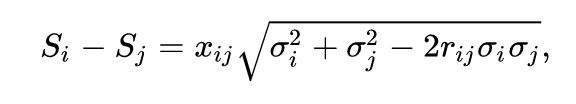
\includegraphics[width=8cm]{graphics/LCJ_formula.png}
	%		\caption{}
	%		\centering
	%	\end{figure}
	
		% $S_{i}$ is the psychological scale value of stimuli $i$
		%{\displaystyle x_{ij}} is the sigma corresponding with the proportion of occasions on which the magnitude of stimulus i is judged to exceed the magnitude of stimulus j
		%{\displaystyle \sigma _{i}} is the discriminal dispersion of a stimulus {\displaystyle R_{i}}
		%{\displaystyle r_{ij}} is the correlation between the discriminal deviations of stimuli i and j
		%The discriminal dispersion of a stimulus i is the dispersion of fluctuations of the discriminal process for a uniform repeated stimulus, denoted {\displaystyle R_{i}}, where {\displaystyle S_{i}} represents the mode of such values. Thurstone (1959, p. 20) used the term discriminal process to refer to the "psychological values of psychophysics"; that is, the values on a psychological continuum associated with a given stimulus.
		
		%However, an alternative version derived from Louis Leon Thurstone, referred to as the "Pairwise Comparison" \cite{thurstone1927law}, will provide an output based on the difference between the quality values is equal to the log of the odds in respect to object-A will be object-B. This formula gets represented as: 
		%$\displaystyle \mathrm {log\;odds} (A\ {\text{beats}}\ B\mid v_{a},v_{b})=v_{a}-v_{b} $.
		
		%$\Pr\{X_{ji}=1\}={\frac {e^{{\delta _{j}}-{\delta _{i}}}}{1+e^{{\delta _{j}}-{\delta _{i}}}}}=\sigma (\delta _{j}-\delta _{i})$
		
		 %.
		%\displaystyle \mathrm {log\;odds} (A\ {\text{beats}}\ B\mid v_{a},v_{b})=v_{a}-v_{b}}		

		How comparative judgement works is to present two options to a marker. The marker then gets asked to pick which one of the two options they think is better. The marker will get presented with all possible combinations available, each picking which one they think is better out of the two. An outputted score is then presented based on the method used, providing a preference order of observations. 
		
		However, an alternative version derived from Louis Leon Thurstone, referred to as the "Pairwise Comparison" \cite{thurstone1927law}, will provide an output based on the difference between the quality values is equal to the log of the odds in respect to object-A will be object-B. This formula gets represented as:
		
		\begin{center}
			 
		$\displaystyle \mathrm {log\;odds} (A\ {\text{beats}}\ B\mid v_{a},v_{b})=v_{a}-v_{b}$ .
		
		\end{center}
	
		Pairwise comparison generally is any process of comparing entities in pairs to judge which of each entity is preferred or has a greater amount of some quantitative property, or whether or not the two entities are identical. The pairwise comparison method get used in the scientific study of preferences, attitudes, voting systems, social choice, public choice, requirements engineering and multiagent AI systems.
		
		Within an educational setting, there have been proposals for a different approach to comparative judgement.  This new adaptation gets referred to as adaptive comparative judgement (ACJ) \cite{pollitt2012method}. It is also the same as the pairwise comparison in concept, just with a different name. ACJ is very similar to the core concept of comparative judgement, as it asks a marker to rate which work is better.  However, in this version, the 'scores', the model parameter for each object, get re-estimated after each 'round' of judgements. Resulting in each piece of work being judged one more time on average. During the next round, each piece of work is compared only to another whose is currently estimated to have a similar score. Therefore, comparing each work with a similar score results in an increased amount of statistical information from each judgment to produce the final ranking. As a result, the estimation procedure is more efficient than random pairing or any other predetermined pairing system like those used in classical comparative judgement applications \cite{pollitt2012method}.
		
		\subsection{What does ACJ aim to achieve and How reliable is it}
		
		Multiple studies have shown that ACJ achieves exceptionally high levels of reliability, often considerably higher than the traditional method of marking. It, therefore, offers a radical alternative to the pursuit of reliability through detailed marking schemes \cite{pollitt2012method}. 
		
		ACJ software estimates a 'measure' for each piece of work getting compared, known as a 'script', and an associated standard error. The process requires several metrics to be measured. These are the true SD, SSR and the index G \cite{ bramley2015investigating}.
		
		The 'true SD' gets calculated for the script by using the formula:
			\begin{center}
				$(True SD)^{2} = (Observed SD)^{2} \text{ - } MSE$
			\end{center}
		 
		The MSE represents the mean squared standard error across the scripts \cite{ bramley2015investigating}. 
		
		The SSR gets defined like reliability coefficients in traditional test theory, as the ratio of true variance to observed variance with the formula \cite{ bramley2015investigating}: 
		\begin{center}
			
		$SSR = (True SD)^{2} / (Observed SD)^{2}$ .
		\end{center}
		Sometimes another separation index G is calculated. Index G represents the ratio of the 'true' spread of the measures to their average error. The formula is \cite{ bramley2015investigating}: 
		\begin{center}
			$G = (True SD) / RMSE$
		\end{center}
		The RMSE is the square root of the MSE. Leading to the SSR, as an alternative, to be calculated as \cite{ bramley2015investigating}:
		\begin{center}
			$SSR = G^2 / (1+G^2 )$
		\end{center}
	
		Studies have found that ACJ has high reliability, even compared to the final results when work is marked more traditional. However,  frustration has been prevalent when markers have had to review repetitive work \cite{bartholomew2019tool}. Additionally, frustration also gets created by the lack of students being able to challenge the final results \cite{bartholomew2019tool}. 
		
		When we look at fig: \ref{fig:studies_comparison}, we can see that these studies have produced a high $SSR$ score. However, a lot of the studies have used a high resource count to complete the different studies. For example, Pollitt 2012 studies used 54 judges to mark 1000 pieces of scripts, which resulted in 8161 different comparisons getting seen and 16 rounds occurring. In comparison, Whitehouse \& Pollit (2012) had 564 scripts to compare and 23 judges. This study took 12 - 13 rounds to get a high SSR score. Therefore, we can see that while ACJ can help with teacher workload in removing a cognitive overload, it takes to create additional workload in the sheer amount of rounds required to get a reliable SSR score.
		
		Additionally, a number of the studies have used 20 - 100 different judges, which is more than most teachers within a single department. Therefore, it makes it hard to see how it can occur within a typical school setup. It brings about questions like, does the requirement needed to produce an accurate judgment outweigh the reduced cognitive load? 
		
		
		\begin{figure}[h]
				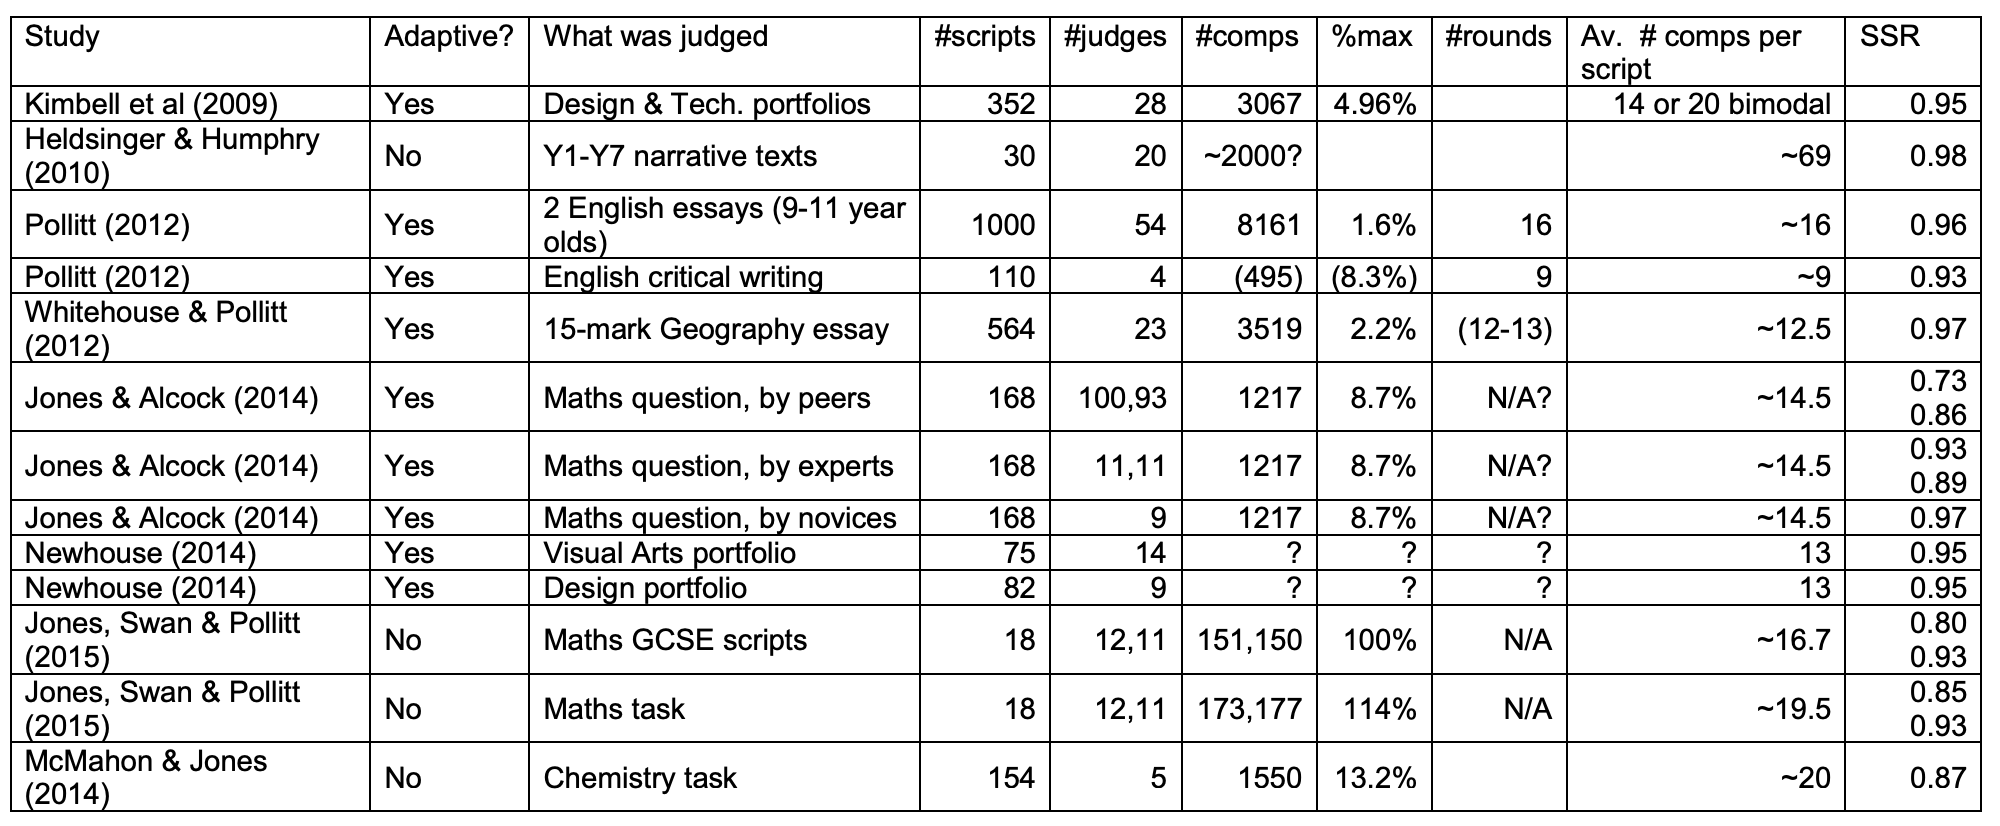
\includegraphics[width=\textwidth]{graphics/cambridge_results.png}
				\caption{Design features and SSR reliability results from some published CJ/ACJ studies \cite{bramley2015investigating}}
				\label{fig:studies_comparison}
				\centering
			\end{figure}
		
		% Negative against ACJ Cambridge Assessment
		Many studies' motivation for using adaptivity in CJ studies is to avoid wasting time and resources by getting judges to make comparisons whose outcome is a foregone conclusion. However, theoretical considerations from the IRT and CAT literature and the simulation study results show that adaptivity produces spurious scale separation reliability, as indicated by values of the SSR coefficient that are considerably biased upwards from their true value. The higher the proportion of adaptive rounds, the greater the bias. SSR values above 0.70 and even as high as 0.89 can get obtained from random judgments \cite{bramley2015investigating}.  
		
		Consequently, the conclusion is that the SSR statistic is misleading and worthless as an indicator of scale reliability. Other reliability indicators, such as correlations with measures obtained from comparisons made among different judges, or correlations with relevant external variables, should be used instead. Therefore ACJ studies that have used high values of the SSR coefficient alone to justify claims that ACJ is a more reliable system than conventional marking need to be re-evaluated \cite{bramley2015investigating}.
		
		
		Additionally, many companies providing CJ tools claim that it only takes  30-seconds to judge a piece of work. However, ultimately the time it will take also depends on the level of the work getting assessed. For example, an A-Level piece of work would take longer than a KS2 assessment. A study where five teachers made 1550 comparisons between them (310 each), and they, on average, took 33 seconds to complete each comparison. Therefore the total marking time was about 2.8 hours per teacher or 14 hours in total. While the two teachers marked the work in a more standard way (using a rubric), taking them 1.5 hours each or 3 hours altogether \cite{mcmahon2015comparative}. Another study claims that CJ requires 17\% more marking time than just using a rubric marking system \cite{steedle2016evaluating}. The results of this comparison of approaches do challenge the efficiency of CJ over standard marking. So if CJ is to become more mainstream within schools, there needs to be a clear benefit for the teachers to adopt this approach. Otherwise, the teachers are less likely to be on board and use the method. As teachers are usually sceptical about new strategies and think they are there to add additional work. However, CJ is recommended for use when the marking is of open-ended exam-style questions \cite{steedle2016evaluating}.
	

	\subsection{How effective is Comparative Judgement at Providing Feedback?} % Should these be subsections?
		Multiple studies have got conducted where ACJ has been used to present feedback to the students. The approach gives students insights into how other people have approached a similar situation differently and how peers valued their work \cite{seery2012validity}. 
		
		ACJ offers a new way to involve all teachers in summative as well as formative assessment. The model provides robust statistical control to ensure quality assessment for individual students through peer assessment \cite{pollitt2012method}. However, while peer feedback is a good strategy, its effectiveness can be limited by the relative students understanding of both the body of knowledge upon which they are getting asked to provide feedback and the skill set involved in providing good feedback \cite{potter2017compair}.
		
		In contrast, a study showed that when peers were involved in synthesising evidence and feedback, the student's engagement in a double looped system of reflection in action increased performance across assignments. Therefore, it indicates that students were receiving feedback to support them in improving their work. The improvements only came from the ACJ judging process, suggesting that students were critiquing their work relative to the breadth of work presented by their peers. They were also engaged in a critique of the purpose of the design assignments concerning core competency development. In essence, students were developing, responding to, and applying criteria \cite{seery2019integrating}.
		
		However, all these examples allow students to gain feedback in a ranked method of how well they have scored against others by seeing other students work modelled to them. However, the students are not getting any truly personalised feedback on what has worked well and what needs improving. Additionally, it relies heavily on students to self-assess and provide their internal improvements, relying on them genuinely understanding the requirements, which would be a meagre chance for less confident, low-achieving students. Therefore, it is a more superficial process and lacks any try impact for methods required in a secondary or sixth form classroom. So we believe that the CJ, while it does remove cognitive loads, actually adds more work for the teacher to provide the basic required information they would need in their classroom to present to the students. 
		
		Therefore, questions are produced on CJ's effectiveness if it takes longer than standard marking and does not provide any tangible form of personalised feedback to the students, resulting in the teacher having to do more work to remove the cognitive workload from the teacher. Is this a trade-off worth making? We find the current methods on offer hard to justify the trade when teachers time is already limited. However, it does have many potentials.
		
	
	\section{Additional Rating Systems}
		While comparative judgment has proven to be a suitable method of ranking pairwise matches of students work over the years, it has its limitations. For example, comparative judgment requires every combination to be compared against, which means for a class of thirty students, accounting for 435 different combinations. Take into account a subject like English, which every student will have to take. A typical school year could have 120, which would mean 7,140 different combinations. That is a lot of time and comparisons that would be required. Therefore, to truly take the cognitive load off a marker or teacher, it would be better to try and have different people sub-sample the work. Then, from the scoring of the sub-samples, use this to generate an overall ranking. In essence, it is creating a competitive scoring system against each other. Two suitable systems to achieve this would be an Elo or Glicko rating system.
	
	\subsection{Elo Ranking System}
		The Elo ranking got first introduced into competitive chess in the 1980s \cite{weng2011bayesian}. However, it got created in the 1960s by Arpad Elo as a replacement for the Harkness System. The Harkness System got used by the United States Chess Federation (USCF) at that time \cite{elo1978rating}. Additionally, the Elo system has gets used as a ranking system for football, American football, basketball as well as eSports like Counter-Strike: Global Offensive and League of Legends \cite{silver2015we, pradhan2020power}.
		
		The Elo system looks at the difference in two players ratings, then serves as a predictor for the match's outcome. The players Elo rating is depicted as a number and will change over time depending on the games' outcomes, with the winners taking points from the losers. However, how many points get awarded is decided upon the difference in ranking between the players. If the higher ranked player wins, only a few rating points get taken from the lower-ranked player. However, if an 'upset win' occurs, when the considerably lower rank player beats the higher rank player, a much greater number of points will be gained to the winner and deducted from the loser. Ultimately, even when 'upset wins' happen, the ranking of the players will reflect the valid scores over time \cite{sullivan2016improving}.
		
		However, there are ways that players who know how the system works can cheat it. These methods include protecting one's rating, selective pairing and ratings inflation and deflation.
		
		Players protecting one's rating discourages game activity for players wanting to preserve their score. In essence, this situation gets created when players are not playing any more games once they are at a high score \cite{friedman2013playing}.  A method against this behaviour is to award an activity bonus combined with the ranking score \cite{edelkamp2021elo}.
		
		Selective pairing is when players choose their opponents, which results in players choosing opponents that the player has the minimal risk of losing. Additions like a k-factor got added, but these do not solve the problem completely \cite{edelkamp2021elo}. Additional implementations have got added, like auto-pairing, which are based on random pairings but have a winner stays on context \cite{edelkamp2021elo}.
		
		
		Inflation is when a score means less over time. For example, a player has a score of 2500 and gets ranked 5, but later, another is ranked 15. It shows that the player's ability is decreasing over time. When deflation happens, this indicates that advancement is happening. Deflation is when a score of 2500, got a player ranking of 7, but at a later date, the score is then put ranked the player 2. Therefore, we must consider when using ratings to compare players between different eras. The ranking gets made more difficult when inflation or deflation are present \cite{williams2013abstracting}. % (See also comparison of top chess players throughout history.)
		
		The Elo system has a flaw in that it is almost certainly not distributed as a normal distribution. As a result, weaker players have greater winning chances than Elo's model predicts \cite{weng2011bayesian}. However, the Elo ratings still provide a valuable mechanism for rating based on the opponent's rating.
	
	\subsection{Glicko Ranking System}
		The Glicko rating system \cite{glickman1995glicko} and Glicko-2 rating system \cite{glickman2012example} are methods for assessing a player's strength in games of skill, such as chess and Go. Mark Glickman invented it to improve the Elo rating system and initially intended it for primary use as a chess rating system \cite{glickman1995glicko}. Glickman's principal contribution to measurement is "rating reliability", called RD, for rating deviation \cite{glickman1995glicko}.
		
		Both the Glicko and Glicko-2 rating systems are under the public domain. Both these systems can get found used on game servers online \cite{williams2013abstracting}. Additionally, the formulas used for the systems are available on Mark Glickman's website \cite{glickman_website}.
	
		The RD measures the accuracy of a player's rating, with one RD being equal to one standard deviation. Then the RD is added and subtracted from their rating to calculate this range \cite{glickman2012example}. Once completion of a game has occurred, the amount the rating changes depends on the RD. The changes are smaller when the player's RD is low,  as the player's rating is already well known. Similarly, when the opponent's RD is high, due to the factor that the opponent's rating is not well known at this point \cite{glickman2012example}. The RD itself decreases after playing a game, but it will increase slowly over time of inactivity \cite{glickman2012example}.
	
	
	\section{Natural Language Processing (NLP)}
		Natural Language Processing (NLP) is a subfield of AI that aims to understand natural language through trying to process and analyse it \cite{vasiliev2020natural, vajjala2020practical}. Ultimately NLP is teaching computers how to understand humans in natural language. However, this is not straightforward, as language is a complex, ever-changing form even for humans. There are three main categories that NLP problems fall into, heuristics, machine learning, and deep learning \cite{vajjala2020practical}. The nature of ML algorithms gets designed to work with unknown datasets, allowing data scientists to learn how to use language \cite{vasiliev2020natural}. While this will bring us a vast amount of insights, as mentioned before, the ever caning landscape of language does not mean that it is perfect and, once made, does not need revision. Therefore generating and understanding natural language are the most promising but most challenging tasks in NLP \cite{vasiliev2020natural, vajjala2020practical}.
		
		To understand the complexities of machines attempting to understand language, we must first know what we mean when we state 'what is language'. Language is a structured communication system, which involves many combinations of its fundamental components of varying complexities. For example, some of these components are characters, words and sentences to name a few \cite{vajjala2020practical}.
		
		\begin{figure}[h]
			\centering
			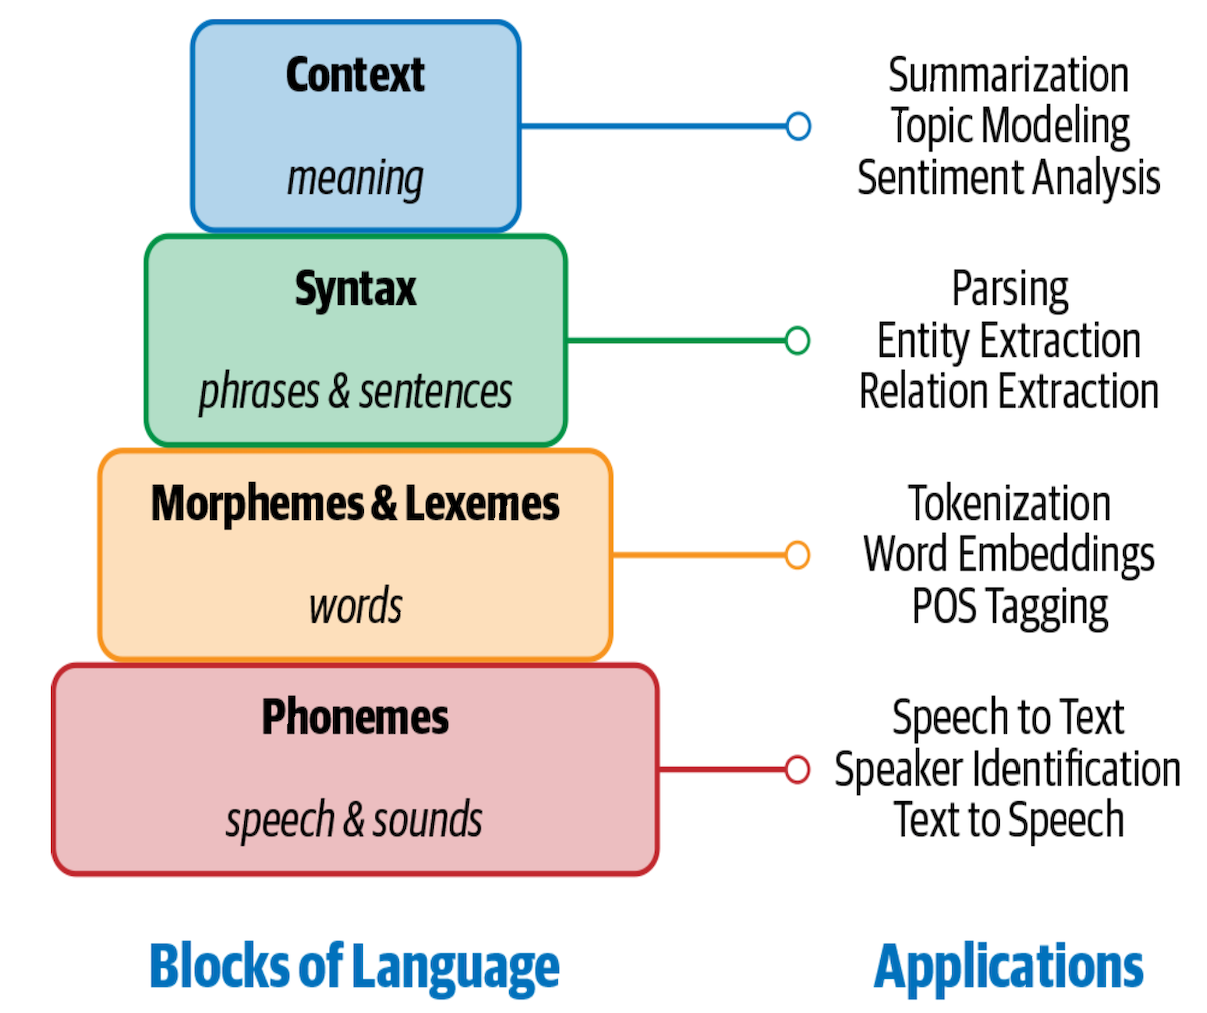
\includegraphics[width=8cm]{practical_building_block.png}
			\caption{This diagram is of the building blocks of language. Additionally, the recommended tools available for understanding the language within applications \cite{vajjala2020practical}.}
			\label{fig:practical_building_block}
			
		\end{figure} 
		
		Human language gets constructed of four major building blocks, and are phonemes, morphemes, lexemes and syntax, and context \cite{vajjala2020practical}. To make an effective NLP app, we need to ensure our application has these different building blocks used within its foundations (see fig: \ref{fig:practical_building_block}). However, knowing these building blocks does not entail we can do what we like within NLP. NLP has many challenges that involve ambiguity, common knowledge, creativity and diversity across languages \cite{vajjala2020practical}. 
	
	
	
	\section{Related Work}
		\label{sec:google_fu}
		
		While comparative judgment is not a new concept, only a few current systems implement a version of it as a tool for marking. These current CJ projects have a slightly different take on the CJ process but have very similar fundamentals. The current offerings are created or provided by RM Compare, a consortium of universities called D-PAC and No More Marking.
		
		RM Compare is probably the version with the most prominent presence. 
		
		\begin{figure}[h]
			\centering
			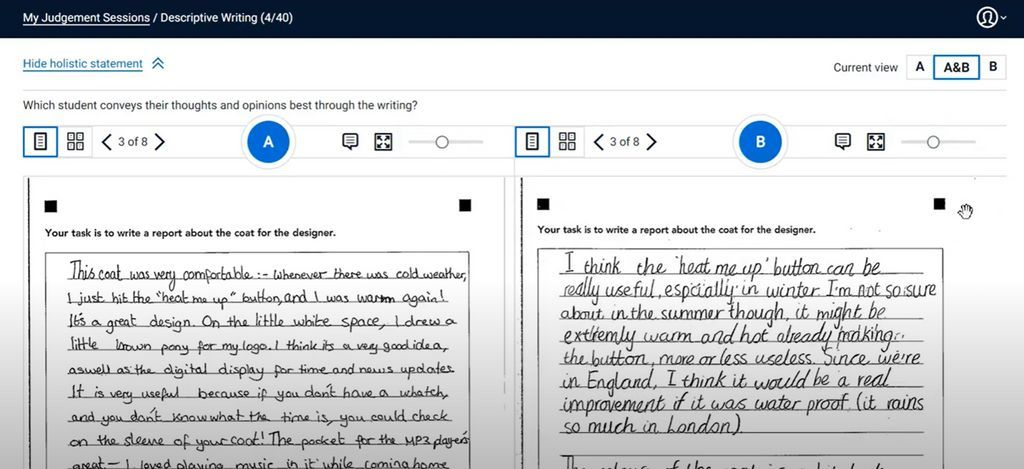
\includegraphics[width=\textwidth]{rm_compare_example.jpeg}
			\caption{RM Compare's ADJ System.}
			\label{fig:rm_compare_ex}
			
		\end{figure}
		
		RM Compare uses ACJ, based on The Law of Comparative Judgement. Two anonymised pieces of work in a side-by-side pairwise comparison is presented to the assessor (a teacher, lecturer, examiner or student). The judge is required to use their professional judgement to select which of the two is better at meeting the assessment criteria (see fig: \ref{fig:rm_compare_ex}).
		
		RM Compare says that through repeated pairwise comparisons, optimised by an iterative, adaptive algorithm, a highly reliable scale or rank order is created through consensus over what 'good', 'better', and 'best' looks \cite{rm_website}.
		
		%[Pros]
		RM Compare empowers users across educational organisations to collaborate on assessments and is proven to increase student attainment. It also reduces the cognitive load from teachers, which gets achieved through the very nature of the comparative judgment process. It also has a straightforward and effective UI for the user to interact with \cite{rm_website}.
	
		%[cons]
		However, it still has an extensive workload as for it to be effective, the markers (known as judges) need to go through several rounds \cite{rm_website}. Multiple examples online were stating 16 rounds. RM Compare states that these numerous rounds are required to reduce the error uncertainty rate.  The algorithm's adaptiveness will ensure that pairs closely matched to each other get checked more to confirm the order is correct, reducing the algorithm's error rate calculation. A high level of uncertainty will get compared more often to check the consensus between the judges \cite{rm_website}. 
	
		An issue with the application is that it does not provide any real form of meaningful feedback. RM Compare suggests that the students gain feedback from the system is for the students to compare their peer's work through the system \cite{rm_website}. Once this comparison by the students gets completed, the students' peered work ranking results will get compared against the teachers \cite{rm_website}. Which then, in turn, gets used as a point of discussion \cite{rm_website}. Therefore, in our opinion, not providing any meaningful form of feedback. While RM Compare that the process has a considerable impact on students attainment, this claim feels more like a marketing gimmick. While we agree that this process can generate insights into students' expectations, it does not provide meaningful, personalised feedback. Therefore, not allowing them to know what they need to do to improve. %ref to RM's website.
		
		\begin{figure}[t]
			\centering
			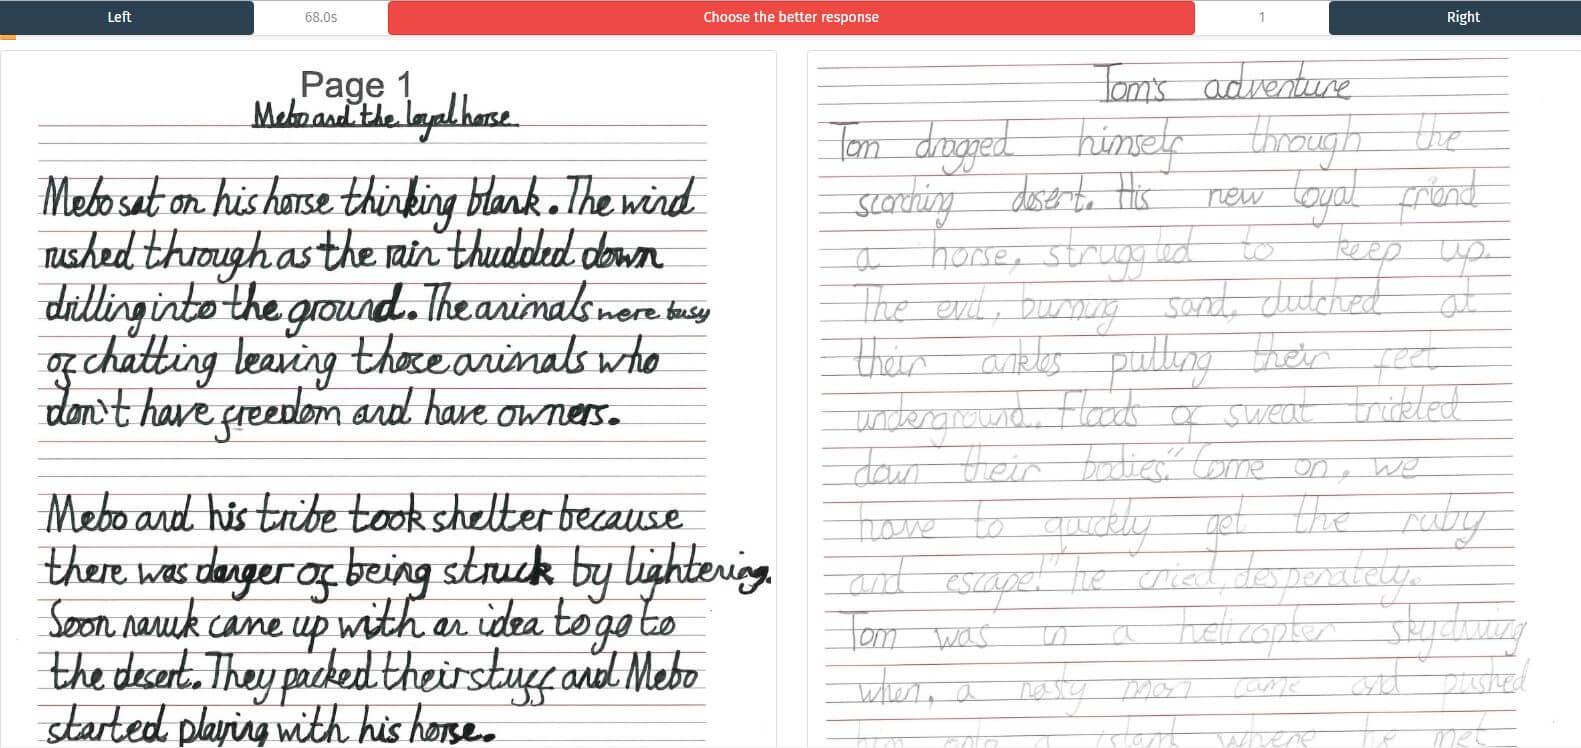
\includegraphics[width=\textwidth]{no_more_example.jpeg}
			\caption{No More Marking's ADJ System.}
			\label{fig:no_more_ex}
			
		\end{figure}
		
		No More Marking is another CJ platform that offers the features of assessing primary writing, improving secondary writing and assessing GCSE English. The company consists of Daisy Christodoulou, who is an influential person within education. She has also received an MBE. Additionally, Dr Christopher Wheadon, Dr Ian Jones, Dr Patrick Barmby, Mr Brian Henderson, Mr Neil Defty.

		No More Marking states that their system uses comparative judgement. 'Which is a process where judges compare two responses and decide which is better. Following repeated comparisons, that result in a statistical model created on the resulting data, and responses placed on a scale of relative quality' \cite{nmm_website}. The No More marking team also claim that 'research has shown the process to be as reliable as double marking, but much quicker \cite{nmm_website}'. However, literature has shown that this is not necessarily true.		
		
		The No More Marking system (see fig: \ref{fig:no_more_ex}) has a very similar layout and design to the RM Compare's version, but we believe with slightly better characteristics. The system is again backed up with research to claim how effective CJ is at marking and how much quicker it can speed up the marking process, which No More Marking have linked to on their website. Additionally, they claim the process is highly reliable. So overall, the system works and acts very similar to RM Compares. As well as claiming a high accuracy and reliability both backed up by research.
		
		However, just like RM Compare's system, No More Marking has the same underlying issues, in our opinion, as they are very similar and are using the same fundamental technology. Additionally, No More Marking's approach to providing feedback allows the students to do their CJ on peer's work. As discussed in the literature, it has many flaws in this approach, especially as it does not provide any personalised feedback to the student on how to improve.  
	
	
		\begin{figure}[t]
			\centering
			
\includegraphics[width=10cm]{d-pac_example.jpeg}
			\caption{D-Pac's ADJ System.}
			\label{fig:d-pac_ex}
			
		\end{figure}
	
		D-PAC has a slightly different focus compared to RM Compare and No More Marking. While D-PAC provides an application (see fig: \ref{fig:d-pac_ex}), its main focus is to provide the ACJ algorithm \cite{d-pac_blog,d-pac_gh}.
		
		D-PAC decided to open-source their algorithms following a meeting with the team developing the Digital Platform for the Assessment of Competences (D-PAC). The D-PAC project is a consortium of Antwerp University, iMinds and Ghent University funded by the Flemish government \cite{d-pac_blog}. The D-PAC consortium had become disappointed with the lack of products to support researchers and assessment practitioners in CJ. Therefore, D-PAC decided to produce an open-source solution for Comparative Judgement that will support their research program and support the growth of research in this field more generally \cite{d-pac_blog}.
		
		Therefore, in comparison, D-PAC has provided the ACJ algorithm that powers No More Marking's platform.

	
	\section{Overall Aim}
		Comparative judgement is a power tool. It can remove much cognitive load from the teacher. It also eliminates the teacher's bias in the marking process, especially when they know whose student they are marking. Teachers can consider how the student has performed over the year instead of how they did in that final piece of work. Potentially takings away the merits of the student's performance at the moment of the exam.
		
		However, the current process of adaptive comparative judgment can reduce the cognitive load with the teacher marking and lessen the potential for bias from the teacher. Current implementations do have their limitations and still create a lengthy process. With some systems still having markers to mark student's work up to, some examples have 16 rounds of marking, which is still very time-consuming. If the stakeholder wants to expand this to a national level, it would not be very effective.
		
		Therefore, we want to look into different methods of ranking students' work that could allow for a crowdsourced way of marking in a CJ style to be implemented. Suggested alternatives are an Elo system ranking. Additionally, we want to create NLP tools that will allow us to interrogate the data and see if there are any patterns within the data and the end rankings. Allowing us to suggest what aspects of the data makes the content get perceived as good.

	% !TEX root = ../thesis.tex
\chapter{Methodology}
	\label{chap:typesetting}
	In order to apply any ML and NLP to the tweet dataset, to see if we could do any information extraction and statistical analysis, we first needed to be able to generate a ranking of the ten tweets we had obtained. We sourced the tweets themed around Brexit on Twitter, and then a pipeline (see fig: \ref{fig:pipeline}) for sourcing peoples preferences of the tweets was created. The pipeline created was handled by the web app. The web app allowed the user to create an account and then compare the tweets. The resulting decision updated the ELO rating for each tweet and the more simplified traditional comparison judgment method. Each user gets only presented five different combinations, ensuring that a single tweet was only seen by the user once.
	
	\begin{figure}[t]
		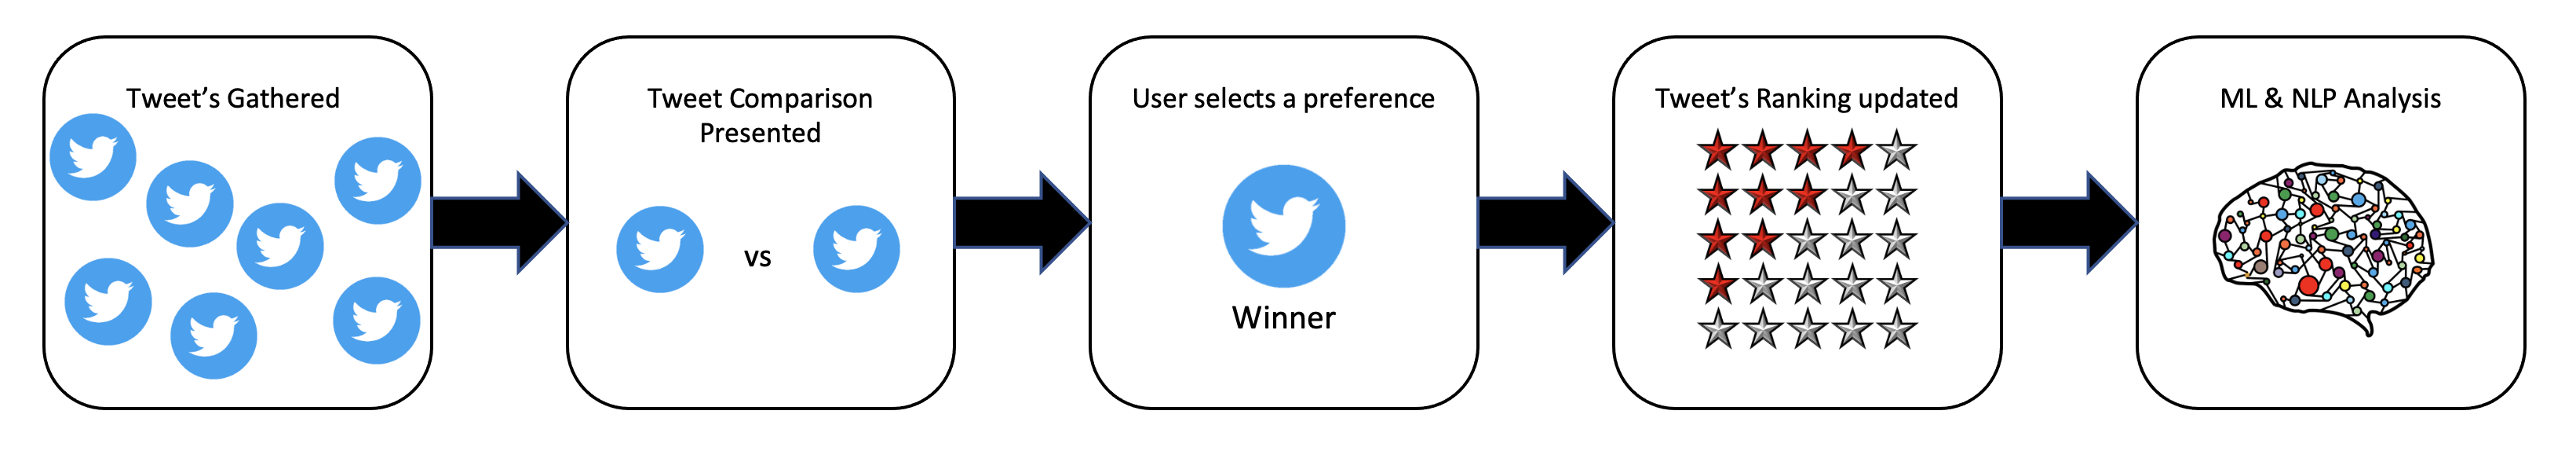
\includegraphics[width=\textwidth]{pipline.png}
		\caption{A visual representation of the processes pipline.}
		\label{fig:pipeline}
		
	\end{figure}
	
	\section{Tools}
	To create the web application and insights from the tweets, we required to use several tools. It is a requirement that we develop a full-stack web application with a user UI, an area to input the user's judgements on the tweet, store the results using a database, and extract information from the tweets using NLP techniques. Several factors within the final application needed to be satisfied for the tools to be appropriate for use.
	
	
	\subsection{Programming Language}
	While many programming languages can handle creating a full-stack application and conducting ML, for example, Java, Php and JavaScript. We decided to use the Python language. We decided upon Python due to our familiarity with it over the other main languages and its versatility. We made this decision because Python can make full-stack applications with the use of additional libraries and handle most NLP ML tasks using libraries like NLTK, SpaCy, Sci-Kit Learn, and TensorFlow.
	
	\subsection{Libraries}
	\subsubsection{Web Application}
	For creating the web application, there were two main libraries available. These were Django and Flask.
	
	Django is a high-level Python Web framework that encourages rapid development and clean, pragmatic design. Built by experienced developers, it takes care of much of the hassle of Web development, so you can focus on writing your app without needing to reinvent the wheel. It’s free and open source \cite{django}.
	
	While Flask is a small framework by most standards—small enough to be called a “micro- framework,” and small enough that once you become familiar with it, you will likely be able to read and understand all of its source code \cite{grinberg2018flask}. 
	
	Flask has three main dependencies. The routing, debugging, and Web Server Gateway Interface (WSGI) subsystems come from Werkzeug; the template support is provided by Jinja2; and the command-line integration comes from Click. These dependencies are all authored by Armin Ronacher, the author of Flask \cite{grinberg2018flask}. 
	
	Flask has no native support for accessing databases, validating web forms, authenti‐ cating users, or other high-level tasks. These and many other key services most web applications need are available through extensions that integrate with the core pack‐ ages. As a developer, you have the power to cherry-pick the extensions that work best for your project, or even write your own if you feel inclined to. This is in contrast with a larger framework, where most choices have been made for you and are hard or sometimes impossible to change \cite{grinberg2018flask}.
	
	%decision and justification
	After experimenting with the two frameworks, we decided upon Flask. Flask got decided upon because of the short time frame to put the project together. Additionally, the lightweight nature of the framework also played a fact as we believe that as this will be just an initial prototype, all the other requirements that Django requires would be unessential additionals to the project. Therefore, taking focus away from what we believe is the main focus. 
	
	\subsubsection{NLP Tasks}
	
	\subsection{IDE}
	
	\section{Software Development Life Cycle Methodology}
	
	
	\section{Data Set}
	
	\subsection{Data Capture Method}
	
	\subsection{Pre-Processing}
	
	
		\section{Implementation}
	[gather tweets]
	
	[Web App]
	The web application got implemented using the Python web library Flask. The web application used several industry-standard tools, for example, HTML, CSS, JavaScript, Bootstrap and dynamic content. The HTML, CSS, Bootstrap and JavaScipt was used to handle the application's front end. 
	
	\begin{figure}[t]
		\centering
		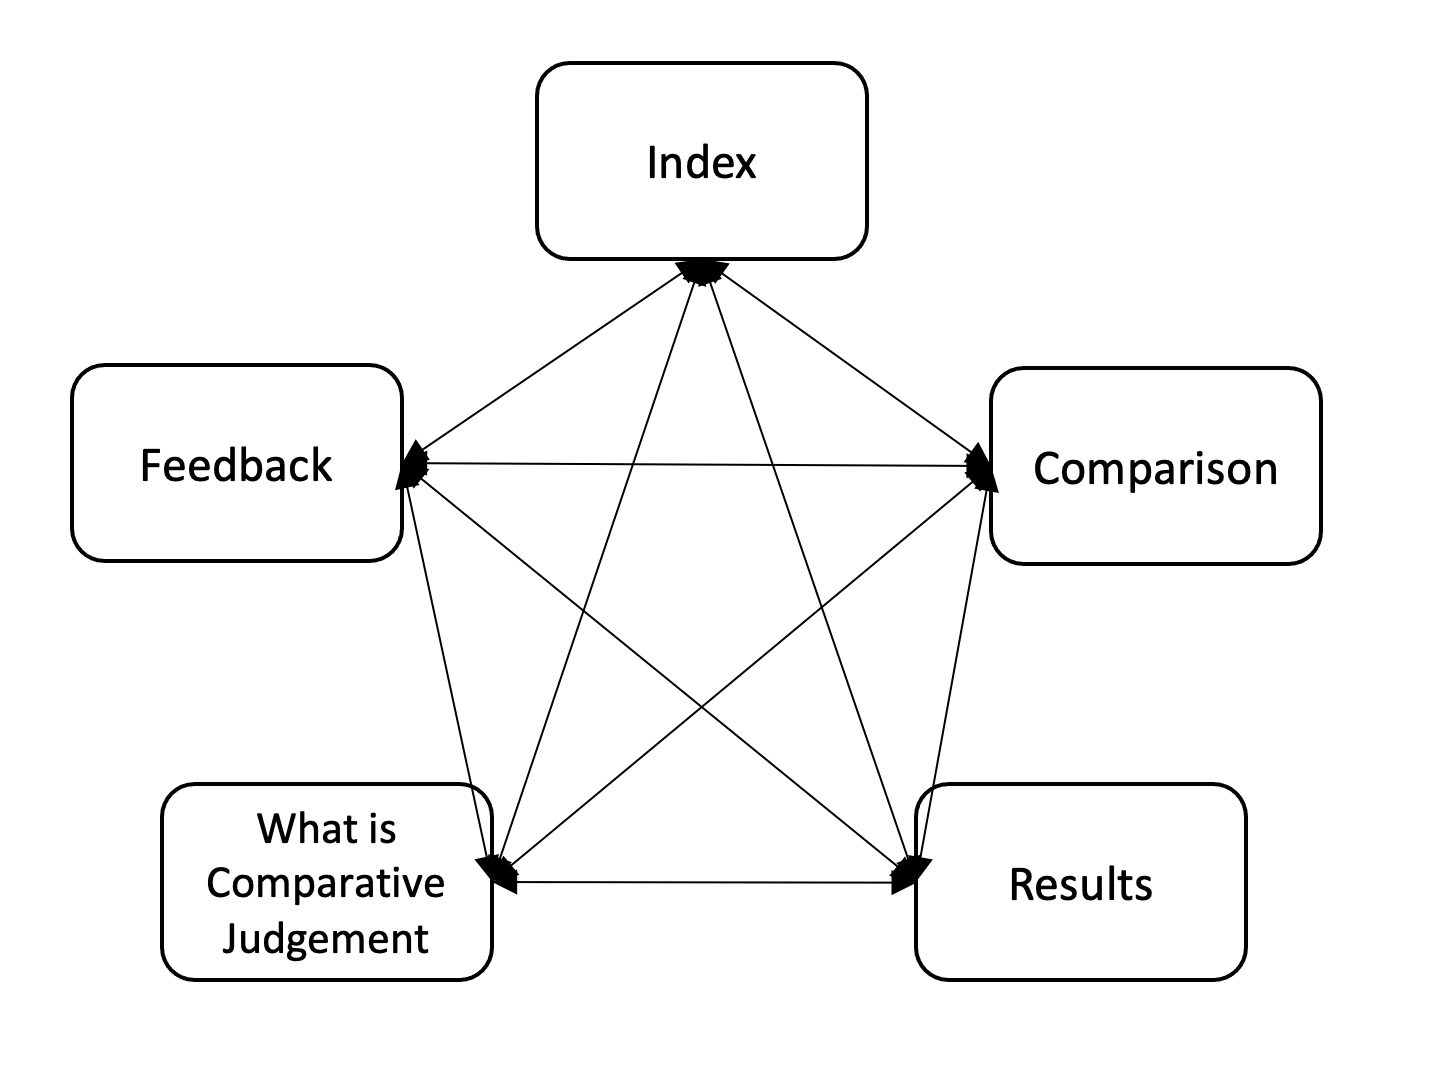
\includegraphics[width=8cm]{web_app_nav.png}
		\caption{A visual representation of the web apps navigation.}
		\label{fig:web_app_nav}
		
	\end{figure}
	
	Additional tools like Google's Firebase was used to handle user authentication and store the web app's content in their real-time databases. The real-time databases are a NoSQL document notation database that updates in real-time. 
	
	Heroku handled the hosting of the web app. Heroku is a free-to-use web hosting provider. However, with it being a free-to-use service, it did bring about some undesirable aspects, mainly the website's slow loading time.
	
	
	
	% !TEX root = ../thesis.tex
\chapter{Results and Discussion}
\label{chap:results}

We will first look at the web application results based on the user's feedback, and then we will look into the insights and potential feedback the NLP process could provide the user. We then also look to review the overall process. 

We will compare the web application's results against the comparative judgment, Elo ranking, and the score we created for the tweets on Twitter. With the insights of the NLP for feedback to the user, we will look at what insights got made. Additionally, we will look at if any of the knowledge extracted generated provides any meaningful feedback to the user.



\section{Tweet Ranking Results} 
\label{sec:reaults_ranking}

	\begin{figure}[h]
		\centering
		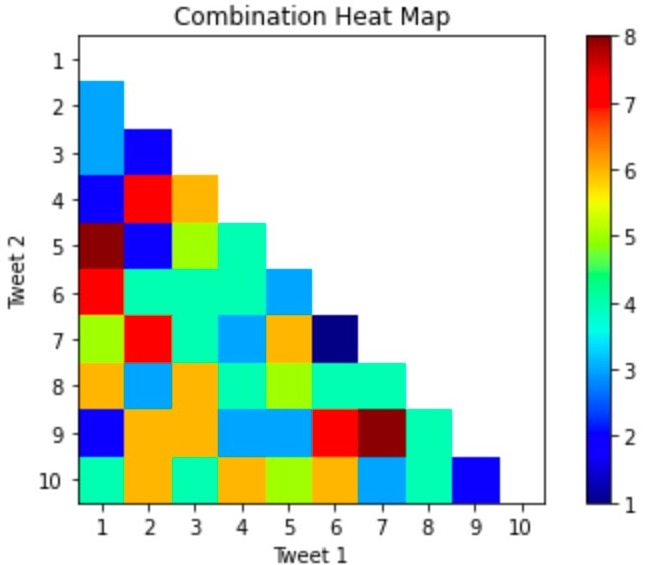
\includegraphics[width=7cm]{combination_heat_map.png}
		\caption{The web applicaitons generated results compared agaist each other.}
		\label{fig:combinations}
		
	\end{figure}
	
	Forty different users take part in the comparison judgement within the web app. Through looking at fig: \ref{fig:combinations} we can see that all combinations got displayed to the users taking part in the comparisons. We can see that tweet one and tweet five appeared the most, while the combination appearing the lowest was tweet six and seven, with one comparison getting presented to the users.
	
	\begin{figure}[t]
		\centering
		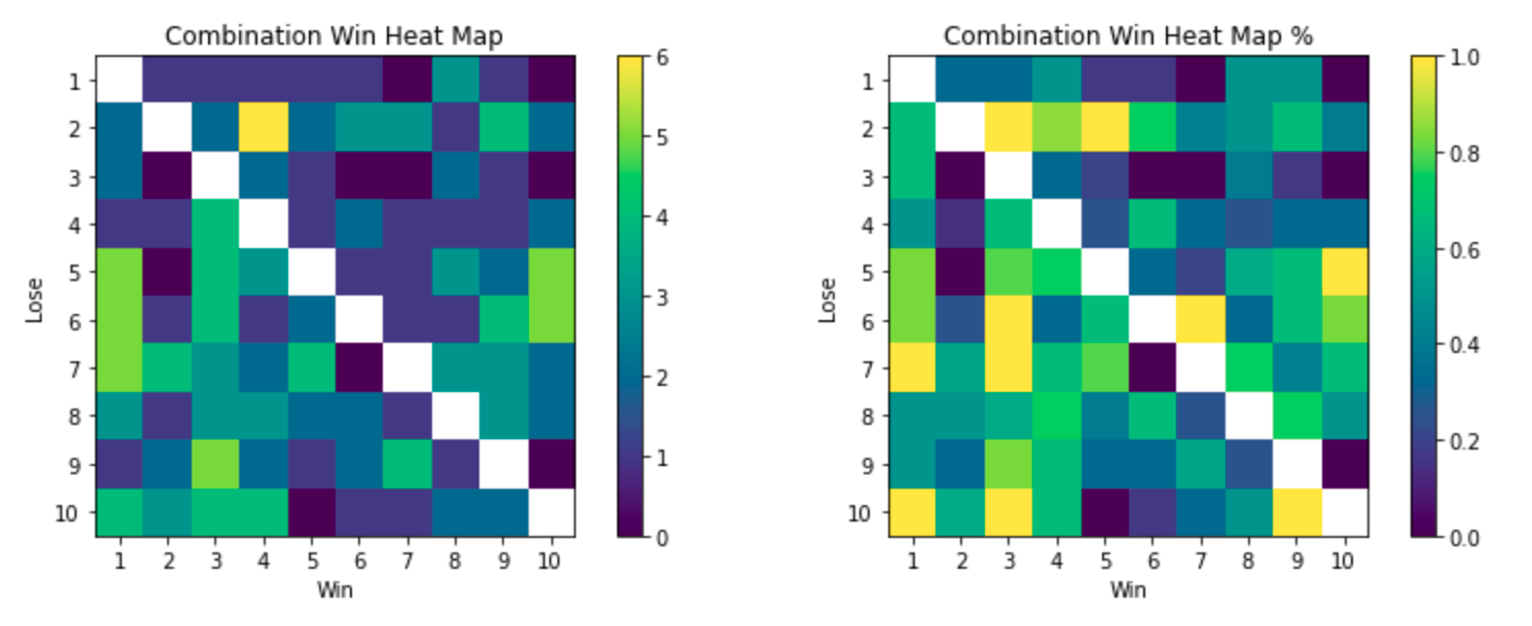
\includegraphics[width=\textwidth]{Combination_win_with_perc_heat_map.png}
		\caption{A heat map of the amount of times a tweet win or lost. Left - by total values. Right - By win percentages.}
		\label{fig:Combination_win_with_perc_heat_map}
		
	\end{figure}
	
	\begin{figure}[b]
		\centering
		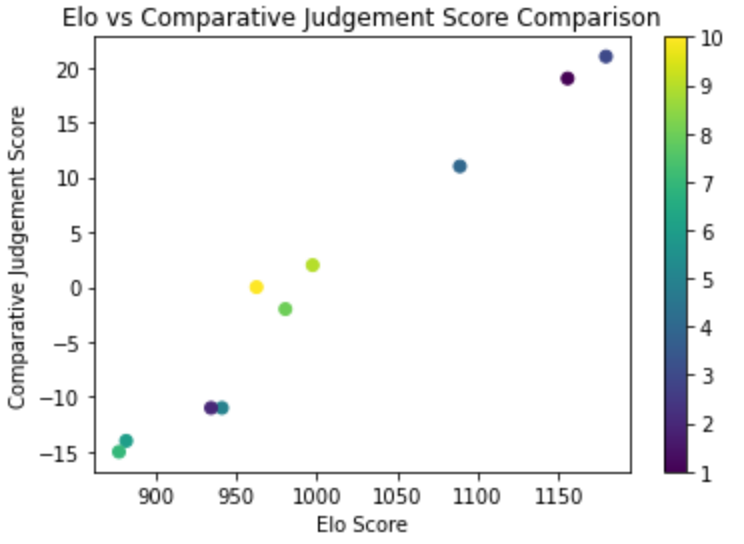
\includegraphics[width=7cm]{elo_vs_cj_comparison.png}
		\caption{A scatter graph plotting each tweet againast their Elo and comparative judgement score.}
		\label{fig:elo_vs_cj_comparison}
		
	\end{figure}
	
	When we look at winners and losers of the comparisons( see fig: \ref{fig:Combination_win_with_perc_heat_map}), we can see that the tweet that won the most between a specific combination was tweet four and two, with tweet four winning six times and tweet two winning only once. Additionally, when we look at the combination that appeared the most, one and five, one came out on top five times, compared to five winning between the two once.
	
	When we look at the winner heat map (see fig: \ref{fig:Combination_win_with_perc_heat_map}), we can see that two, five, six, seven and ten had moments where they didn't win a head-to-head with another tweet. Two, six, seven and ten didn't win against at least two different tweets, while the others were only against one tweet they failed to win.
	
	%\begin{figure}[h]
	%	\centering
	%	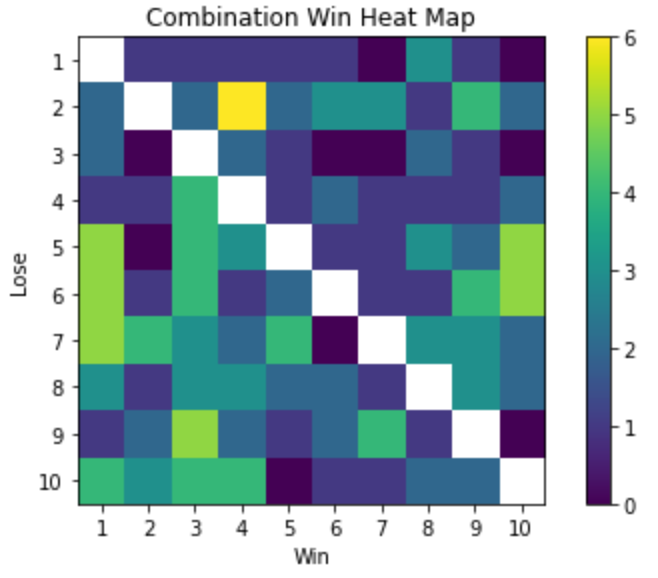
\includegraphics[width=7cm]{combination_win_heat_map.png}
	%	\caption{A heat map of the amount of times a tweet win or lost.}
	%	\label{fig:combination_wins}
		
	%\end{figure}
	
\begin{figure}[t]
	\centering
	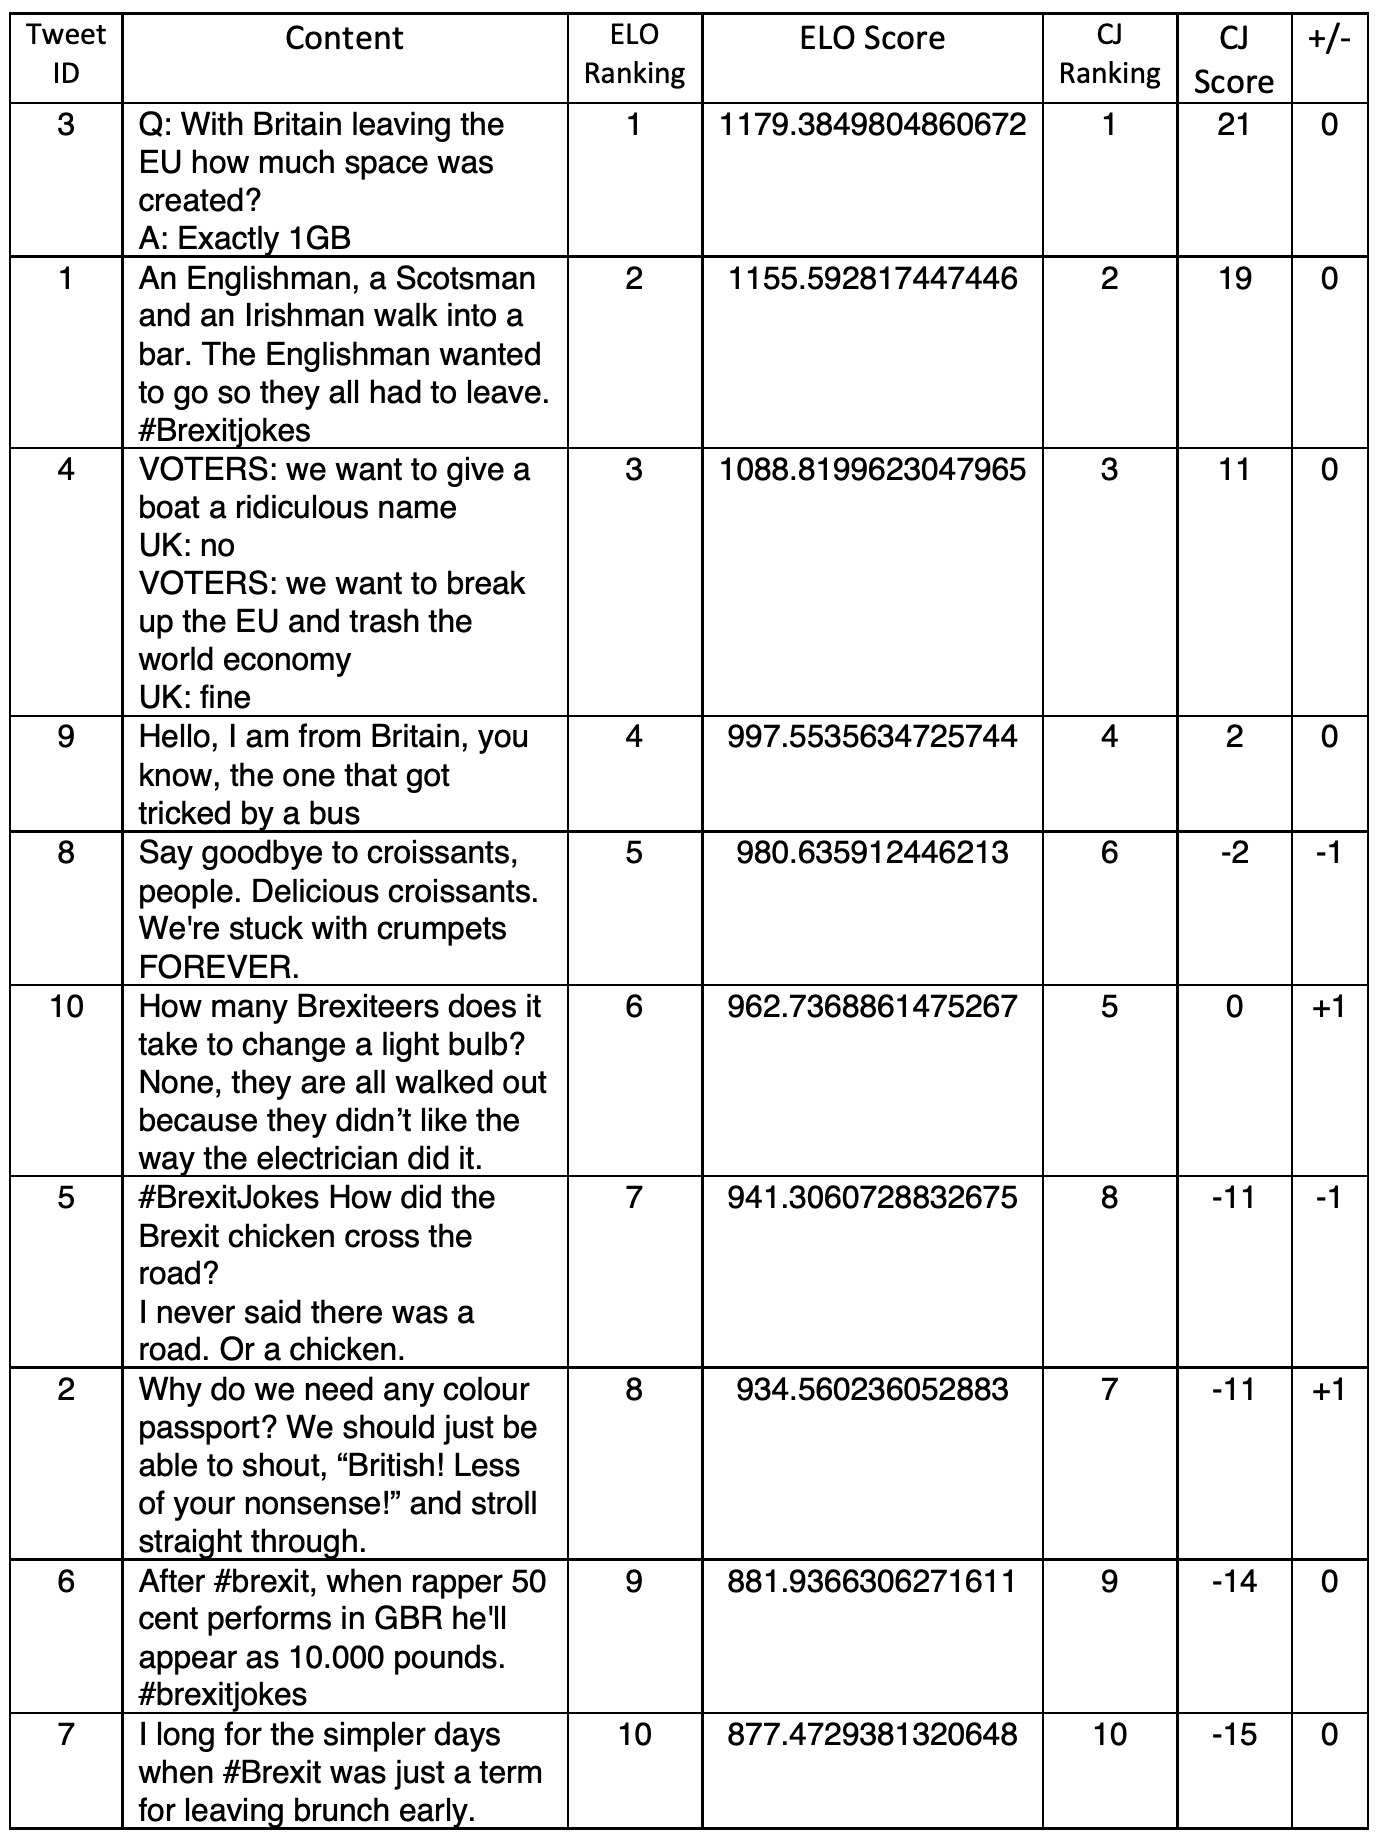
\includegraphics[width=10cm]{web_app_results.png}
	\caption{The web applicaitons generated results compared agaist each other.}
	\label{fig:web_app_results}
	
\end{figure}
	

	When we look at the two scores plotted against each other, Elo and CJ (see fig: \ref{fig:elo_vs_cj_comparison}), it shows that these values are linearly correlated. Additionally, the results returned as 0.98391595 when a Pearsons correlation test got conducted on these scores. Therefore, the two values are heavily linked, so when a tweet has a good Elo score, it also has a good CJ score. This correlation between the results shows that the Elo score is an excellent alternative to the CJ scoring system. Through using the Elo system, also provides the process with a lot more robustness. It allows the ranking to get done to a high degree of accuracy. Additionally, without every combination getting presented against each other. As a result, this would be a sound scoring system to implement at a national scaled-up scale.

	While looking at fig \ref{fig:web_app_results}, we can see that the Elo and comparative judgement ranking generated very similar results. However, as we can see, the tweets coming in 6th, 7th and 8th a slight variation in the results.
	
	\begin{figure}[t]
		\centering
		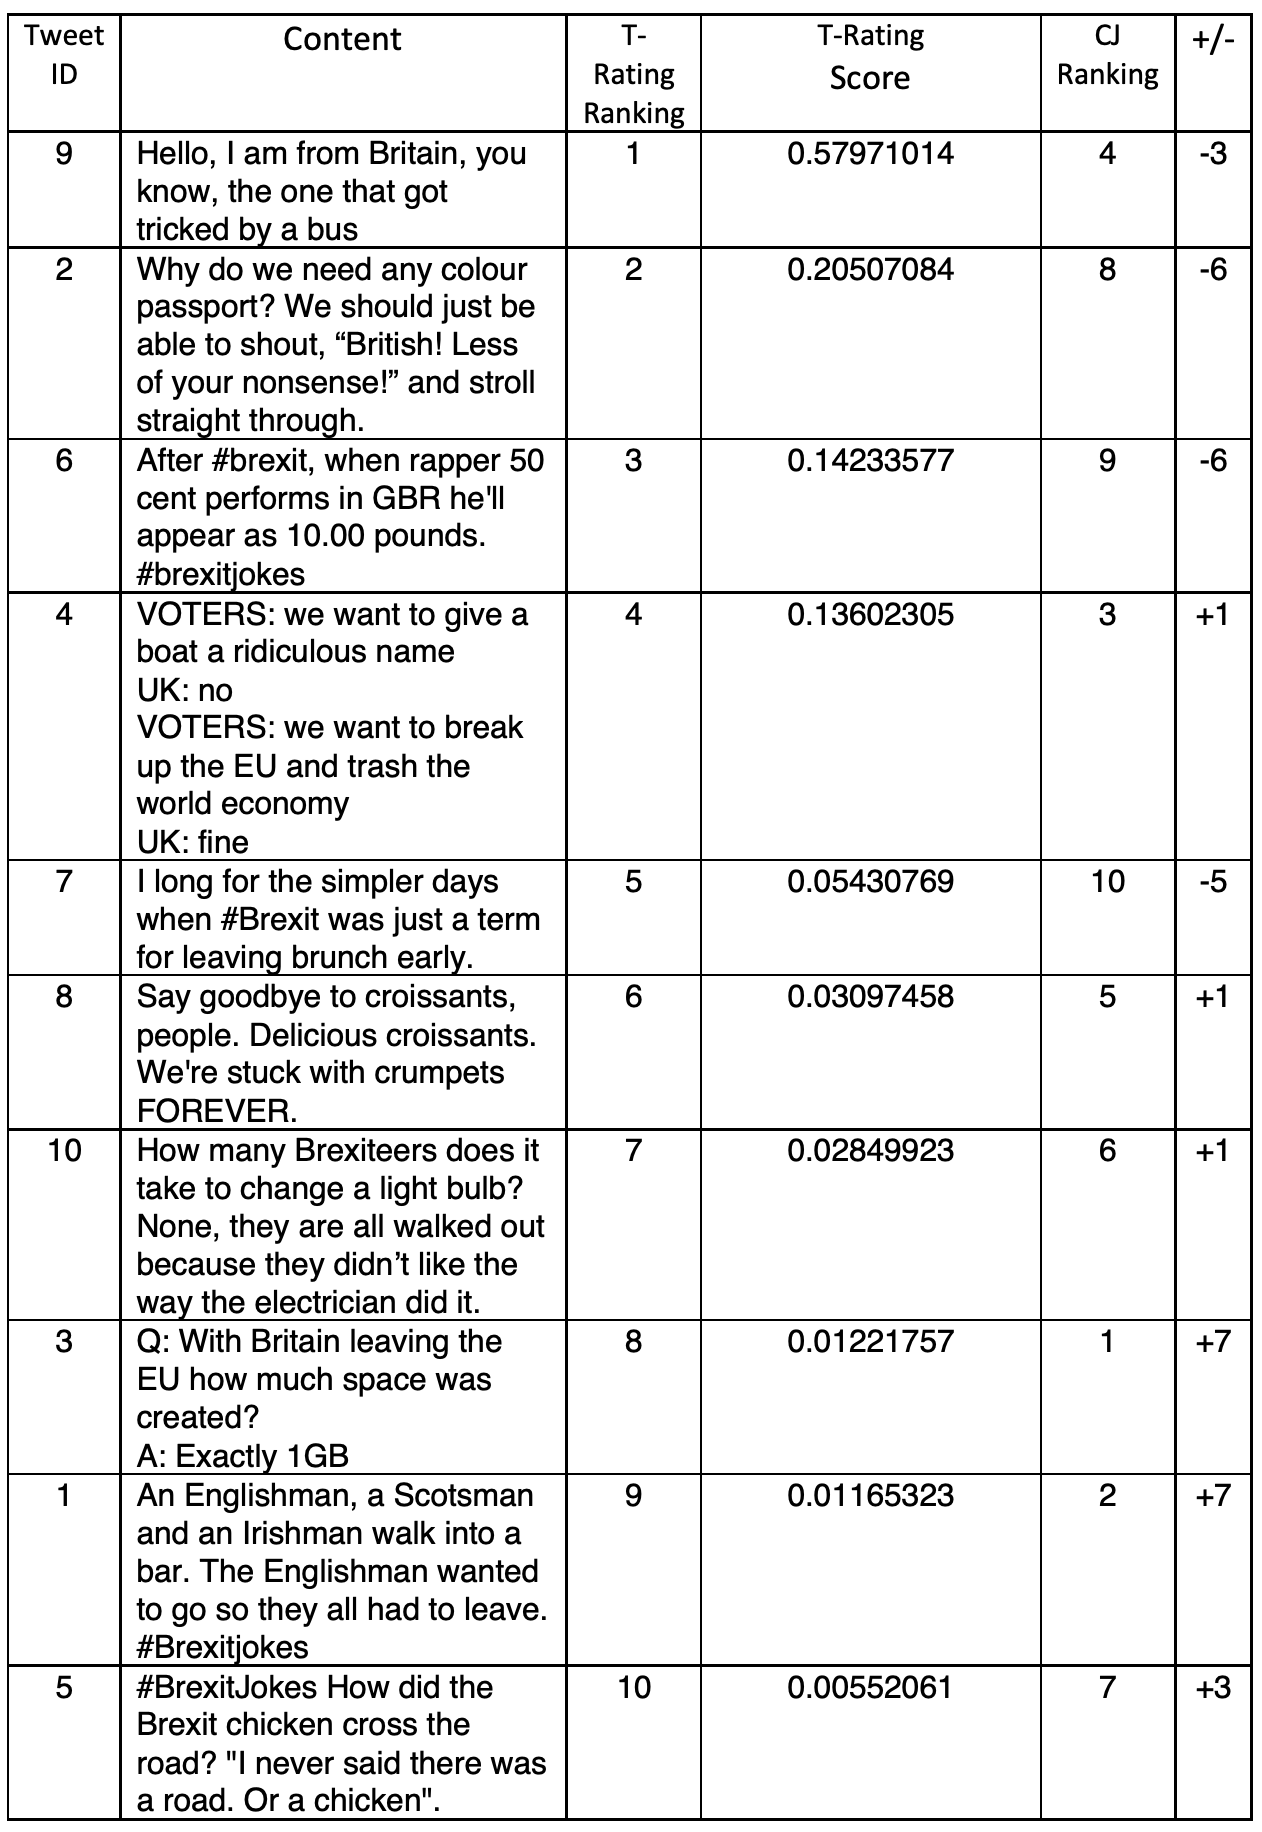
\includegraphics[width=10cm]{twitter_results_comparison.png}
		\caption{The Twitter tweet score ranking comparison against Elo ranking.}
		\label{fig:twitter_results_comparison}
		
	\end{figure}

	While we look at the T-rating ranking compared to the Elo ranking (see fig: \ref{fig:twitter_results_comparison}), we can see that the results ranking is very different. The tweet that came first in the T-rankings came fourth in the Elo ranking. At the same time, the tweet that came first in the Elo ranking came eighth in the T-ranking.  Tweets that done worse in the Elo ranking compared to T-ranking had an average difference in the ranked placing of 5 places, while the tweets that had a better Elo ranking compared to the T-ranking ranked an average of 4 places lower. Therefore, 4 of the top 5 tweets in the T-ranking were actually in the bottom five of the Elo ranking. Only tweet ID 4 done one place better with the Elo ranking than it did in the T-ranking. However, two of the top three tweets in the T-ranking were in the bottom three of the Elo ranking and vice versa.
	
	However, even though these ended up with very different results, due to the multiple variables at play regarding Twitter, in terms of likes, retweets, followers, how many followers retweeters have, a tweet might have, the random chance of someone seeing it. The T-rating system is a very ambiguous metric to use as an accurate ranking system. Additionally, with Twitter being a global app, the results on certain tweets could be affected by people's views from outside the UK, drastically changing opinions. Another factor that is making this a difficult comparison to make is the sample size. The tweets on Twitter had many more people interacting with them than how many people took part in our study. Therefore, how the tweet did in the real world is not a valid comparison against the Elo rankings results. There is also room to suggest that this proves that the Elo system is better suited for this action, as it can handle random chance elements regarding its pairings. 
	
	However, this comparison has brought to light a valid point: do we want the results to be decided upon by a local group of specialised people? Or do we want the results to get agreed upon as a global element? For example, teachers within a school in the UK would possibly be looking for different work factors compared to a teacher in Finland. Therefore, creating contrast in views. Additionally, GCSE awards bodies might also have different focuses within their assessments, even when it comes to subjects like English. So this could have a huge impact on views getting generated around the ranking of students work which would need further investigating.

	Within the forty participants, twenty-two of them left a justification for why they select one tweet over the other. However, the participants' responses were varied in the amount of provided feedback. Some proved a justification for all five combinations. On the other hand, some only left them for a few and not all. The users gave a total of sixty-three explanations to their decisions on which tweet they had chosen.
	
	One user stated, "I just think it is a clever way to put our departure from EU, plus it did make me giggle." The comment was in regards to tweet three beating tweet eight. Tweet three did provide several justifications, a lot of them to do around its tech theme on Brexit. Some of the rationales are "Comp sci wordplay", "everyone loves a tech joke", "Because it's the nerdier option", the "First tweet just lol", and "Actually laughed out loud".
	
	Another tweet, tweet ten beating tweet 8, had the justification for winning as 'because of the wordplay'. So we can see that several tweets had some form of explanation around the lines of good wordplay. Therefore, creating user feedback has not made an excellent source of information to help build feedback. However, it has given some context to why they had made their decisions.


\section{NLP Feedback and Insights}
\label{sec:reaults_NLP}
	
	The Jupyter notebook was able to conduct the NLP tasks that we required successfully. We presented the user the POS tagging insights of how many POS tags were present in each tweet. We were also able to visualise the POS tagging to reflect the user how the tweet got broken down structure-wise (see fig: \ref{fig:POS_example}).
	
	\begin{figure}[h]
		\centering
		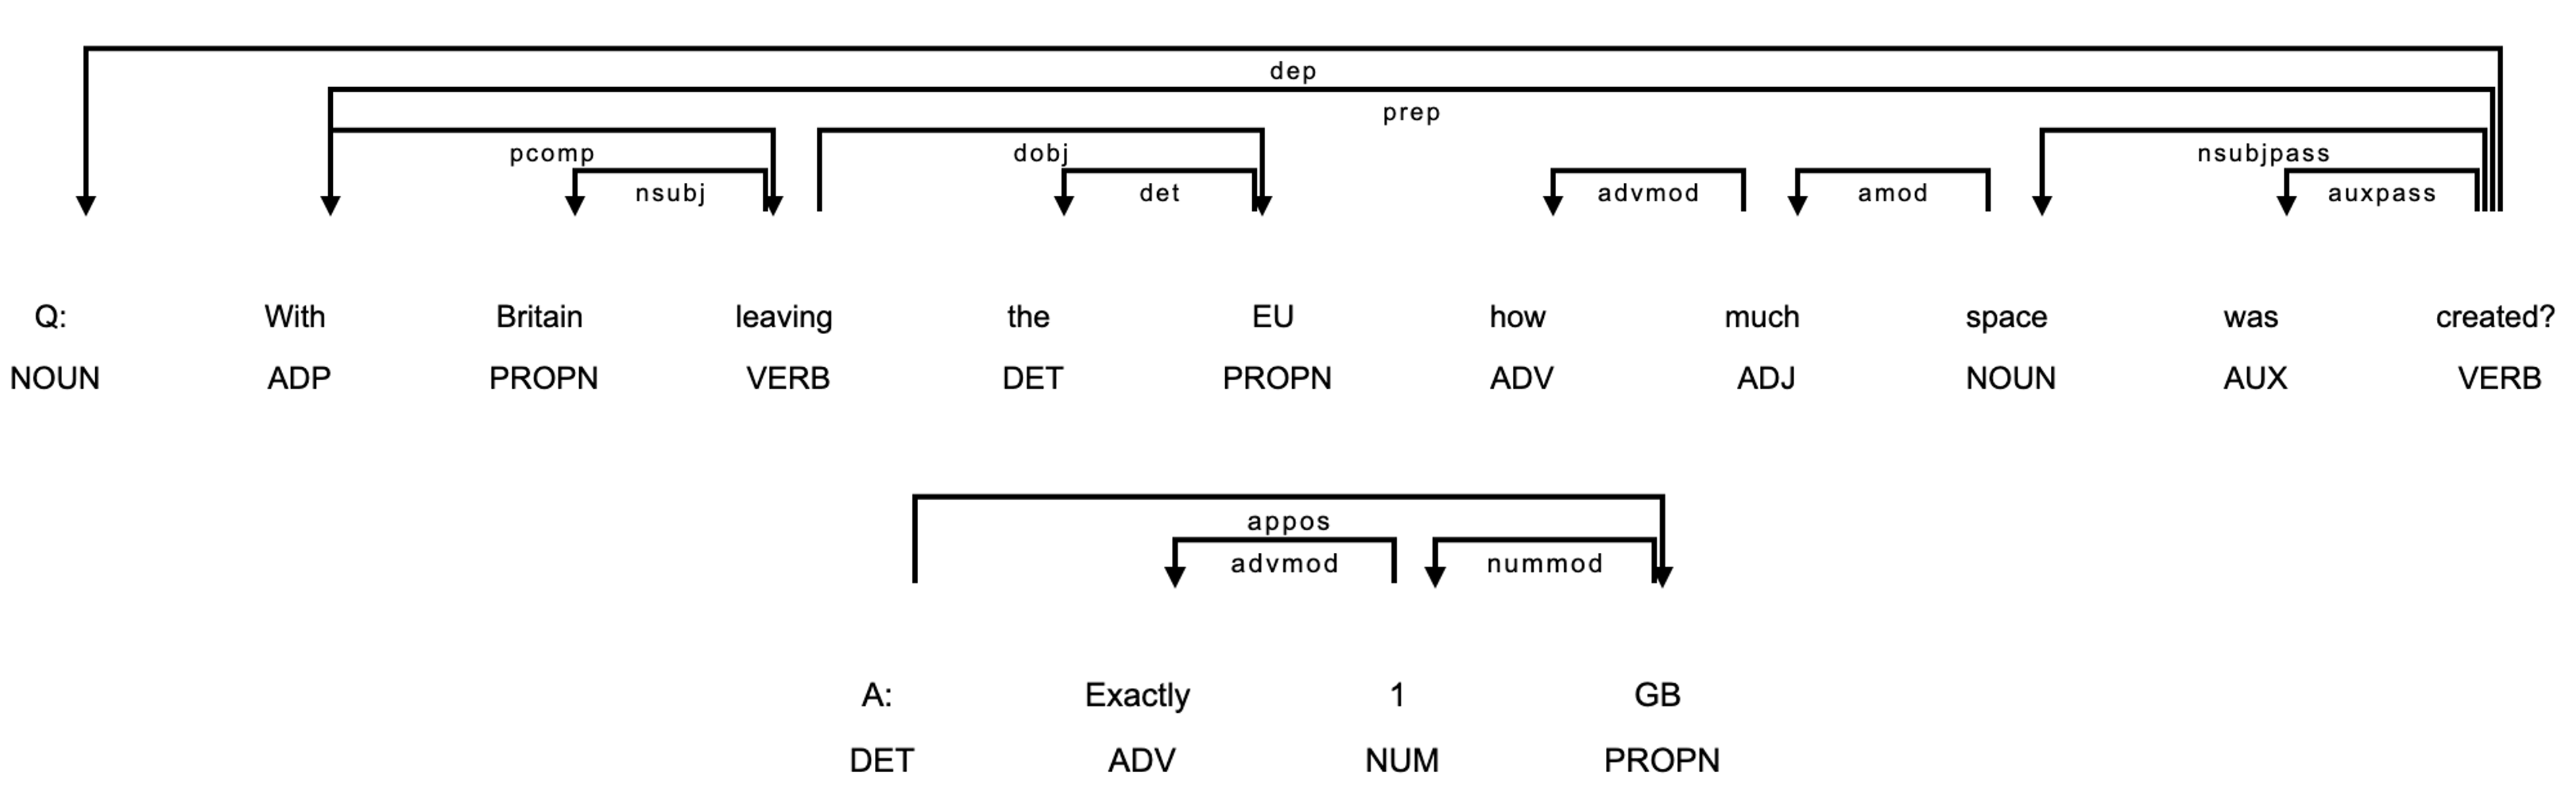
\includegraphics[width=\textwidth]{POS_vis.png}
		\caption{An example of a POS tagging visulaisation.}
		\label{fig:POS_example}
		
	\end{figure}

	We were also able to present to the user the NER that the pre-trained model supplied by spaCy was able to identify. These were presented to the user in text format as well within a visualisation, identifying the NERs within the sentence (see fig: \ref{fig:NER_example}).
	
	\begin{figure}[h]
		\centering
		
\includegraphics[width=\textwidth]{NER_vis.png}
		\caption{An example of a NER tagging visulaisation.}
		\label{fig:NER_example}
		
	\end{figure}

	The notebook was also able to present back to the user the top ten tweets on how similar they were by the whole tweet (see fig: \ref{fig:top_10_sim_doc}) and by NERs (see fig: \ref{fig:top_10_sim_NER}). When looking at the results for the similarity scoring between the NERs, we can see that the most similar tweets are tweet three and tweet 4. These tweets have a similarity score of 0.857896 based on the NER values Britain, EU (Tweet 1) and UK, EU (Tweet 4). The tweets with the least similarity are Tweet 2, British, and Tweet 6, 50, cent, 10.00, pounds, with a similarity score of -0.025753.
	 
	
	\begin{figure}[h]
		\centering
		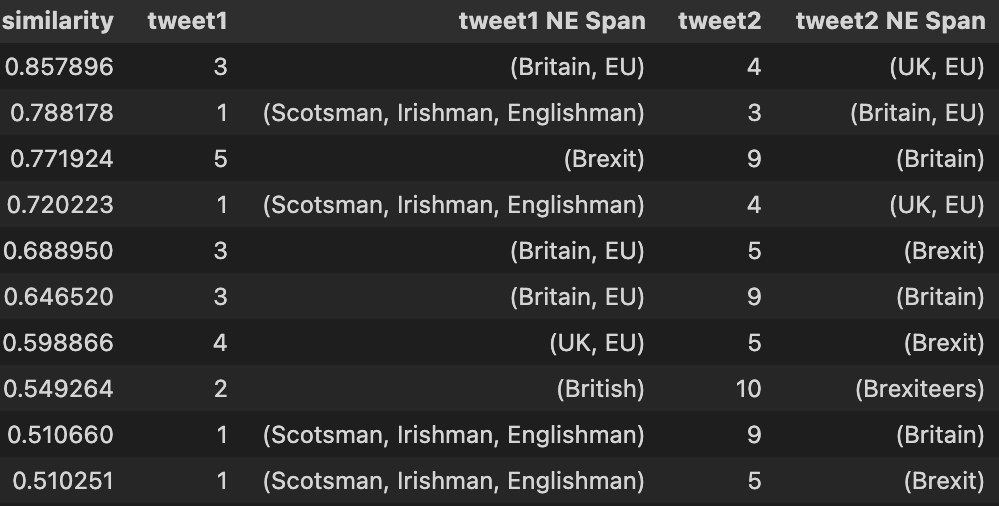
\includegraphics[width=10cm]{top_10_sim_NER.png}
		\caption{A table displaying the top ten similar tweets based on the tweet's NERs.}
		\label{fig:top_10_sim_NER}
		
	\end{figure}

	The results show us, in regards to the whole tweets, that Tweet 5 and Tweet 10 were the most similar with a similarity score of 0.576191. The tweet's contents were '\#BrexitJokes How did the Brexit chicken cross the road? "I never said there was a road. Or a chicken".' (Tweet 5) and 'How many Brexiteers does it take to change a light bulb? None, they are all walked out because they didn't like the way the electrician did it.' (Tweet 10). The tweets with the least similarity are Tweet 4, 'VOTERS: we want to give a boat a ridiculous name UK: no VOTERS: we want to break up the EU and trash the world economy UK: fine', and Tweet 6, 'After \#brexit, when rapper 50 cent performs in GBR he'll appear as 10.00 pounds. \#brexitjokes', with a similarity score of -0.041637.

	\begin{figure}[h]
		\centering
		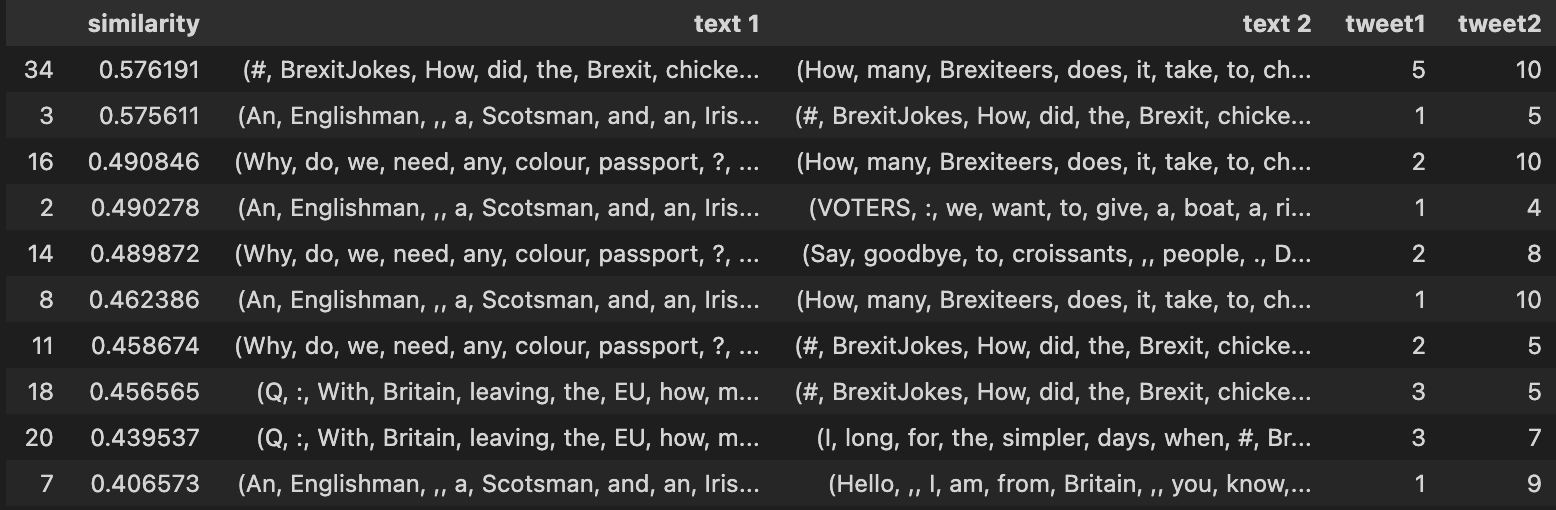
\includegraphics[width=15cm]{top_10_sim_doc.png}
		\caption{A table displaying the top ten similar tweets based on the whole tweet.}
		\label{fig:top_10_sim_doc}
		
	\end{figure}

	The information extraction process identified several interesting aspects from the tweets (see fig: \ref{fig:information_extract}). The results show that six of the tweet's sentiments scoring got classified as positive, and out of those six, five were in the top 5 results. We can't say for certain that having a positive tweet will likely score higher, as the dataset is not big enough to make that kind of claim. However, it does provide some good feedback and insights to the user. The NLP process also provided some excellent extraction of key phrases from the tweets. The only tweet's key phrase that didn't prove any meaningful information was Tweet 7's 'Brexit was'. Considering that these information extraction techniques, NER and key phrases, have not had any additional training, other than what comes out of the box, they have performed well in providing insights and feedback to the user.


	\begin{figure}[h]
		\centering
		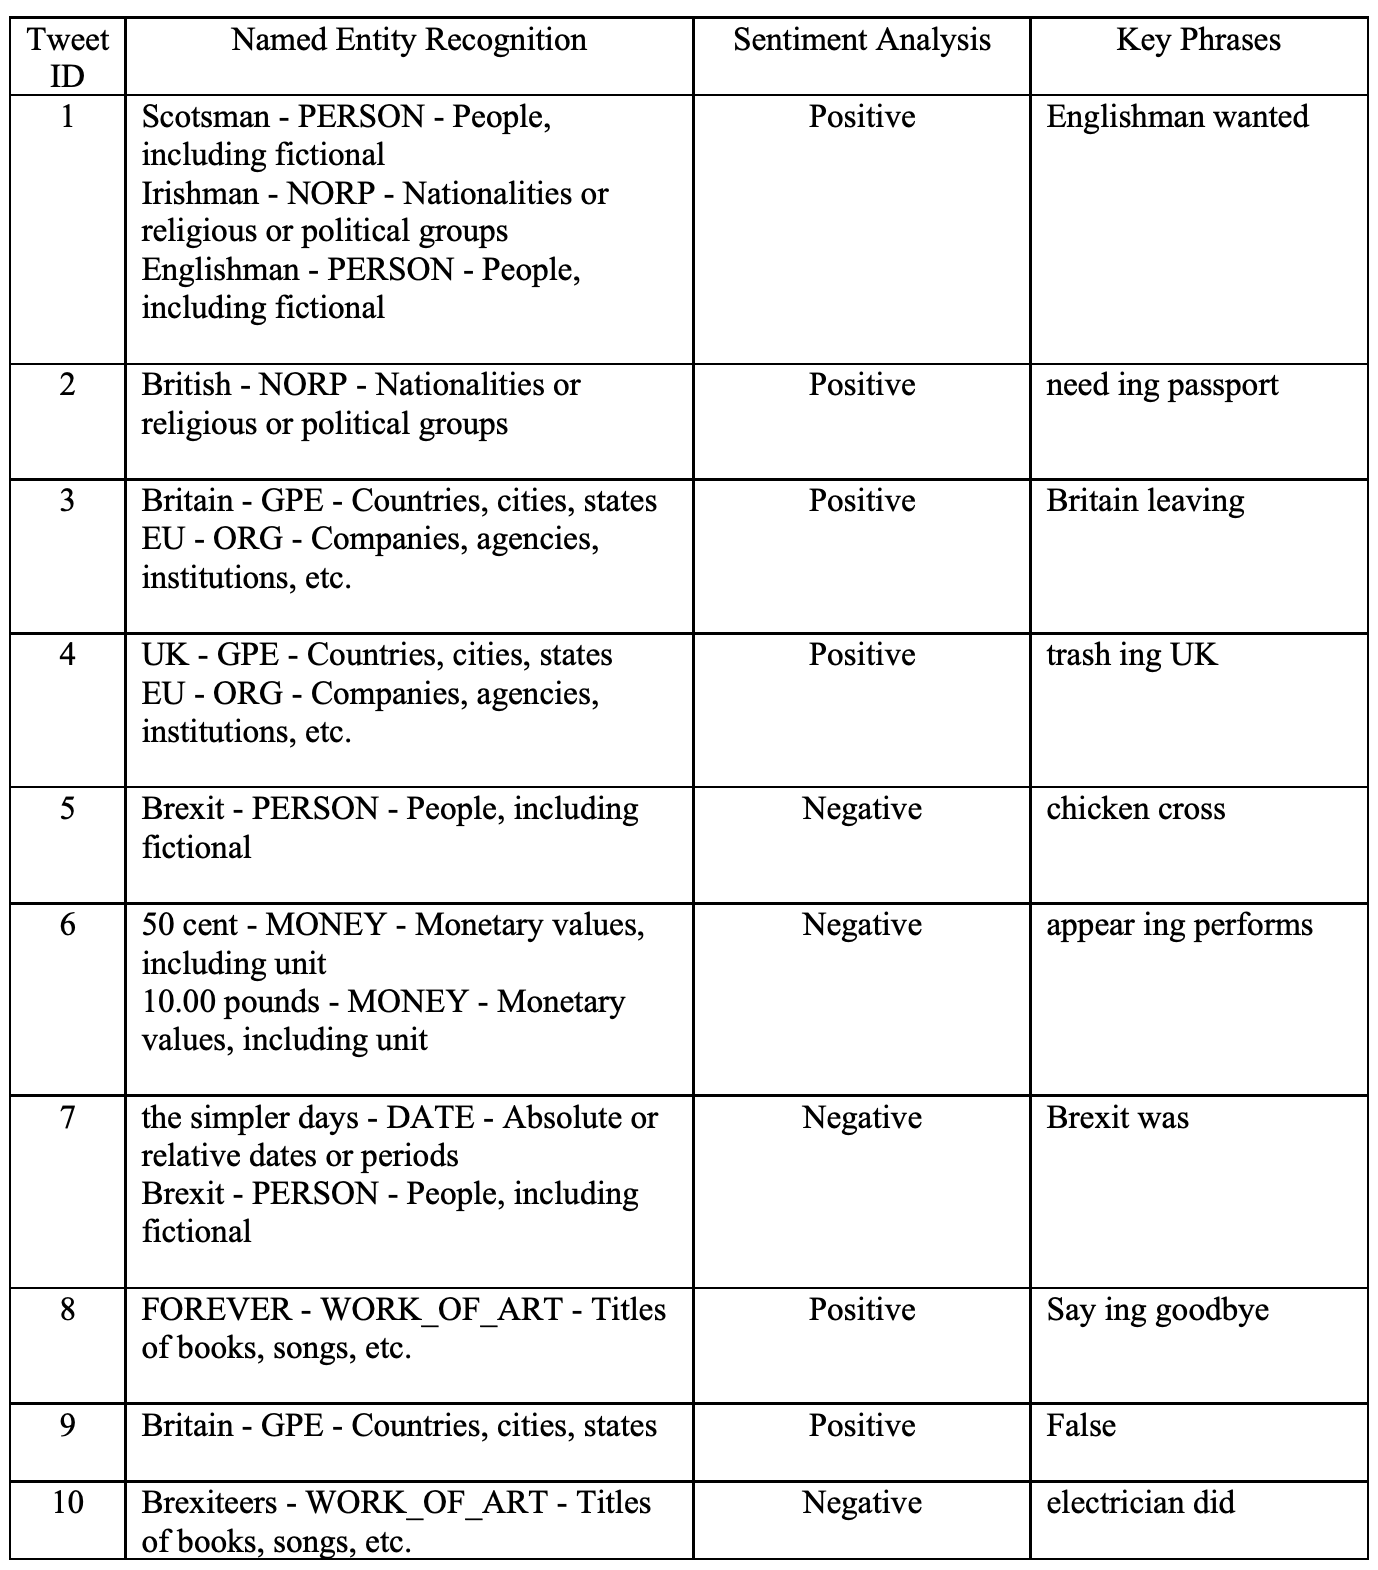
\includegraphics[width=10cm]{information_extract.png}
		\caption{A table displaying the key information extracted from the NER, Sentiment analysis and Key Phrases NLP processes.}
		\label{fig:information_extract}
		
	\end{figure}

	Using the TF-IDF, we extracted the key token features from all of the tweets. The higher the value, the more important that feature is for that tweet (see fig: \ref{fig:feature_extract}). However, this information does not provide much feedback for a user, but it would highly likely be adequate for training some form of ML models.

	\begin{figure}[h]
		\centering
		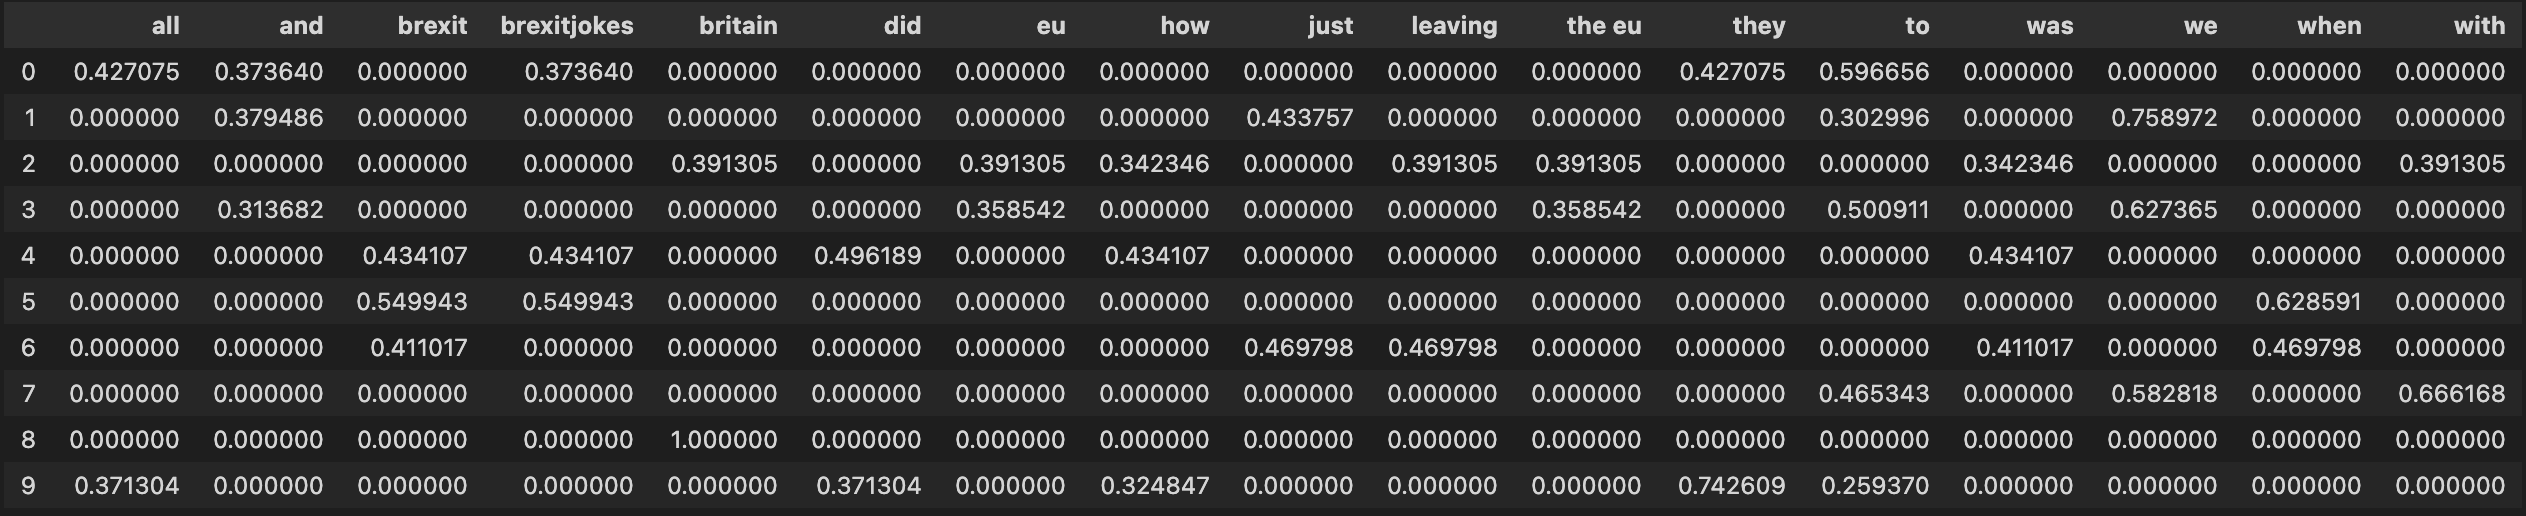
\includegraphics[width=\textwidth]{feat_extra_importance.png}
		\caption{A table showing the key tokens within each tweet and thir importance to that tweet.}
		\label{fig:feature_extract}
		
	\end{figure}

	In contrast, the information extraction techniques of finding word sequence patterns and utterance pattern matching did not provide any meaningful information. The finding word sequence pattern presented only "he'll appear" about Tweet 6, and the utterance pattern matching showed that a pattern was found in Tweet 6 too. These techniques have not provided much use currently but could be helpful when scaling up and using a much bigger dataset, like exam papers.



\section{Overall Results}
\label{sec:reaults_NLP}

	Overall we can suggest that the Elo ranking is a great alternative ranking system to the ACJ. It provides a robust scoring system because the combination process is random, removing any opportunity for Elo's flaws to be taken advantage of. It also provides the ability to try 'what if' calculations with potential comparison outcomes.
	
	On the other hand, the NLP information extraction provided some good information but was too basic to offer any real insights to the user to digest easily. While there is a lot of promise regarding the NLP, more fine-tuning is required to make this feature to provide feedback worthwhile. However, we believe this is a step worth taking with appropriate building blocks that have been put in place to expand upon.


	% !TEX root = ../thesis.tex
\chapter{Conclusions and Future Work}
\label{chap:conclusion}


The process of CJ is undeniable in reducing cognitive load, as our brains are much more adapt to comparing one thing to another and saying one is better. The literature around CJ firmly claims that ACJ is a better alternative to more traditional marking methods, for example, using a rubric. CJ does have several flaws. One of the flaws is that the whole process can take longer than traditional marking in the first place. Additionally, the adaptive nature of ACJ can generate bias within its results by getting the markers to mark more often, especially when the results get closely ranked to each other. It gets claimed that a random pairing is better than the adaptive approach. A considerable flaw within the CJ/ACJ process is that it does not provide personalised feedback to the learners. Giving feedback is a vital part of education today, ensuring that students know where they are and where they need to improve. Instead, CJ's feedback approach is to allow students to peer-assess each other and then gain their insights from their understanding. However, this relies on the students understanding the marking criteria in the first place and extracting what they need to improve on.

While CJ generates results to create a ranking of the students' work, CJ is not the only ranking method available. Multiple ranking systems can get used within competitive chess and e-Sports. Two such methods are the Elo and Glicko ranking. While the Glicko system is a proposed improved system over Elo, the Glicko system introduces features that we did not need, and the flaws within the Elo system would not get abused within our proposed solution. Therefore we decided to use the Elo ranking system.

Therefore, we created a web app that allowed users to compare two tweets and declare what tweet they prefered. The results then got used to calculate a simplified CJ score and an Elo score, allowing us to compare the final results of the two ranking systems. Additionally, a Jupyter notebook got created to carry out information extraction techniques. These techniques include POS tagging, NER, feature extraction, sentiment analysis, text similarity scoring, utterance pattern matching, finding word sequence patterns and finally extracting key phrases.

The results from the web app presented that the final Elo ranking and the CJ score a strongly correlated, with a score of 0.98391595. The web app allowed the users to complete the comparisons very quickly and only do one round of judgements. Therefore, reducing cognitive load and reducing the time required for marking. However, the scores only became truly useful after several users had completed the comparison. Still, the more users took part, the more sure the final results became, with the results showing that the Elo system is a suitable method for ranking the results.

In contrast, when we compared Elo's scores ranking against the T-rating, these did not correlate with each other. However, we believe that this is not a very straightforward comparison, but it does bring up questions to think about. For example, do we want a selection of specialised local markers to conduct the CJ in the future or is using a global approach ok? Also, how would the outcome be with a larger sample size getting used, rather than the 40 users who took part?

While the web app generated a strong argument for using the Elo ranking system, the NLP notebook for information extraction did not provide the exact outcome we expected. While the notebook did complete all the NLP tasks we required, it did produce some good insights into the tweets. It did not manage to provide any real insights that an end-user could use to provide personalised feedback. However, it did create great building blocks to build upon.

Overall, the research ended up with many positives, but some areas need development, especially when providing feedback using NLP techniques. However, the study has shown that the Elo system has a solid case for getting used for ranking work. As it massively reduces the time required to complete compared to ACJ methods. Additionally, the process also being based around CJ reduces the cognitive load for anyone taking part in the judging. Therefore, we believe there is much potential within combining these techniques.


\section{Contributions} 
\label{sec:intro_contribs} 

The main contributions of this work are as follows: %The main contributions of this work can be seen as follows:

\begin{description}	
	
	\item[\(\bullet\) A web application to conduct the comparative judgement]\hfill
	
	We created a web application and hosted it to crowdsource users views on ten tweets based on Brexit. The app provided at random five unique pair comparisons while updating the CJ score and Elo score. 
	
	\item[\(\bullet\) A comparison of two different ranking systems]\hfill
	
	Metrics are being stored and calculated based on the two ranking systems, a CJ style and an Elo ranking system. Therefore, the results provide us with a way to compare the effectiveness of the two ranking systems. As a result, they are allowing us to see which one works better in our required situation.
	
	\item[\(\bullet\) An exploration into NLP techniques to provide feedback to the user]\hfill
	
	We created a Jupyter notebook exploring NLP information extraction techniques to provide feedback to the user from information extracted from the ten tweets.
	
\end{description}

% original
%\begin{description}	

%	\item[\(\bullet\) A \LaTeX{} thesis template]\hfill

%Modify this document by adding additional top level content chapters.
%These descriptions should take a more retrospective tone as you include summary of performance or viability. 

%	\item[\(\bullet\) A typesetting guide for useful primitive elements]\hfill

%Use the building blocks within this template to typeset each part of your document.
%Aim to use simple and reusable elements to keep your document neat and consistently styled throughout.

%	\item[\(\bullet\) A review of how to find and cite external resources]\hfill

%We review techniques and resources for finding and properly citing resources from the prior academic literature and from online resources. 

%\end{description}


\section{Future Work}
\label{sec:conclusion_future_wk}

While the research found some good insights, we believe much future work can get done. We believe a bigger pool of samples needs to occur for the Elo system to be assured as an alternative to the ACJ method. Additionally, introducing the markers and seeing how long it takes for the sample pool to be marked and how well it ranks against a more traditional rubric marking method.


More work can be done with the Elo score and converting the results into grades from A* to F. We believe that a process can convert the results created by the Elo score into standardised GCSE grades. For example, an Elo score greater than 1800 is equivalent to an A*, or a score greater than 1700 resulting in an A grade.

However, where we feel a lot more research can get done is within the NLP capabilities. We believe that the ability to extract the information from a student's work and then provide personised feedback would be a fantastic addition to the CJ process. Therefore, allowing teachers to reduce their cognitive load and workload, as giving feedback would take a time consuming and draining task away from them. Having the NLP processes automated, but allowing the teacher to have overall control, would be a massive addition to any teacher's toolbox. Ultimately reducing their workload and allowing the teacher to do what they are best at, creating engaging lessons for their students.


% Insert the bibliography using citations contained in the file citations.bib
	\bibintoc % Whether to list the bibliography in the Table of Contents (or: \nobibintoc)
	\bibliography{citations} 
	
% In the appendix you might include a full code listing for an implemented algorithm 
% that you showed a small chunk of in one of your chapters. If you have extra graphs 
% you might enumerate them within the appendix and use \label{name} and \cref{name} 
% to automatically insert the correct section locations when you talk about them in your 
% chapters. It is *not* necessary to include all of your implementation code as an 
% appendix; instead, focus on the important highlights so they do not get drowned out.
% Within appendix.tex you should use chapters as the top level section dividers.
	\ifdraftdoc\else
	\appendix
	\addappheadtotoc
	% !TEX root = ../thesis.tex
\chapter{Web App Pages}
\label{app:web_designs}

\begin{figure}[h]
	\centering
	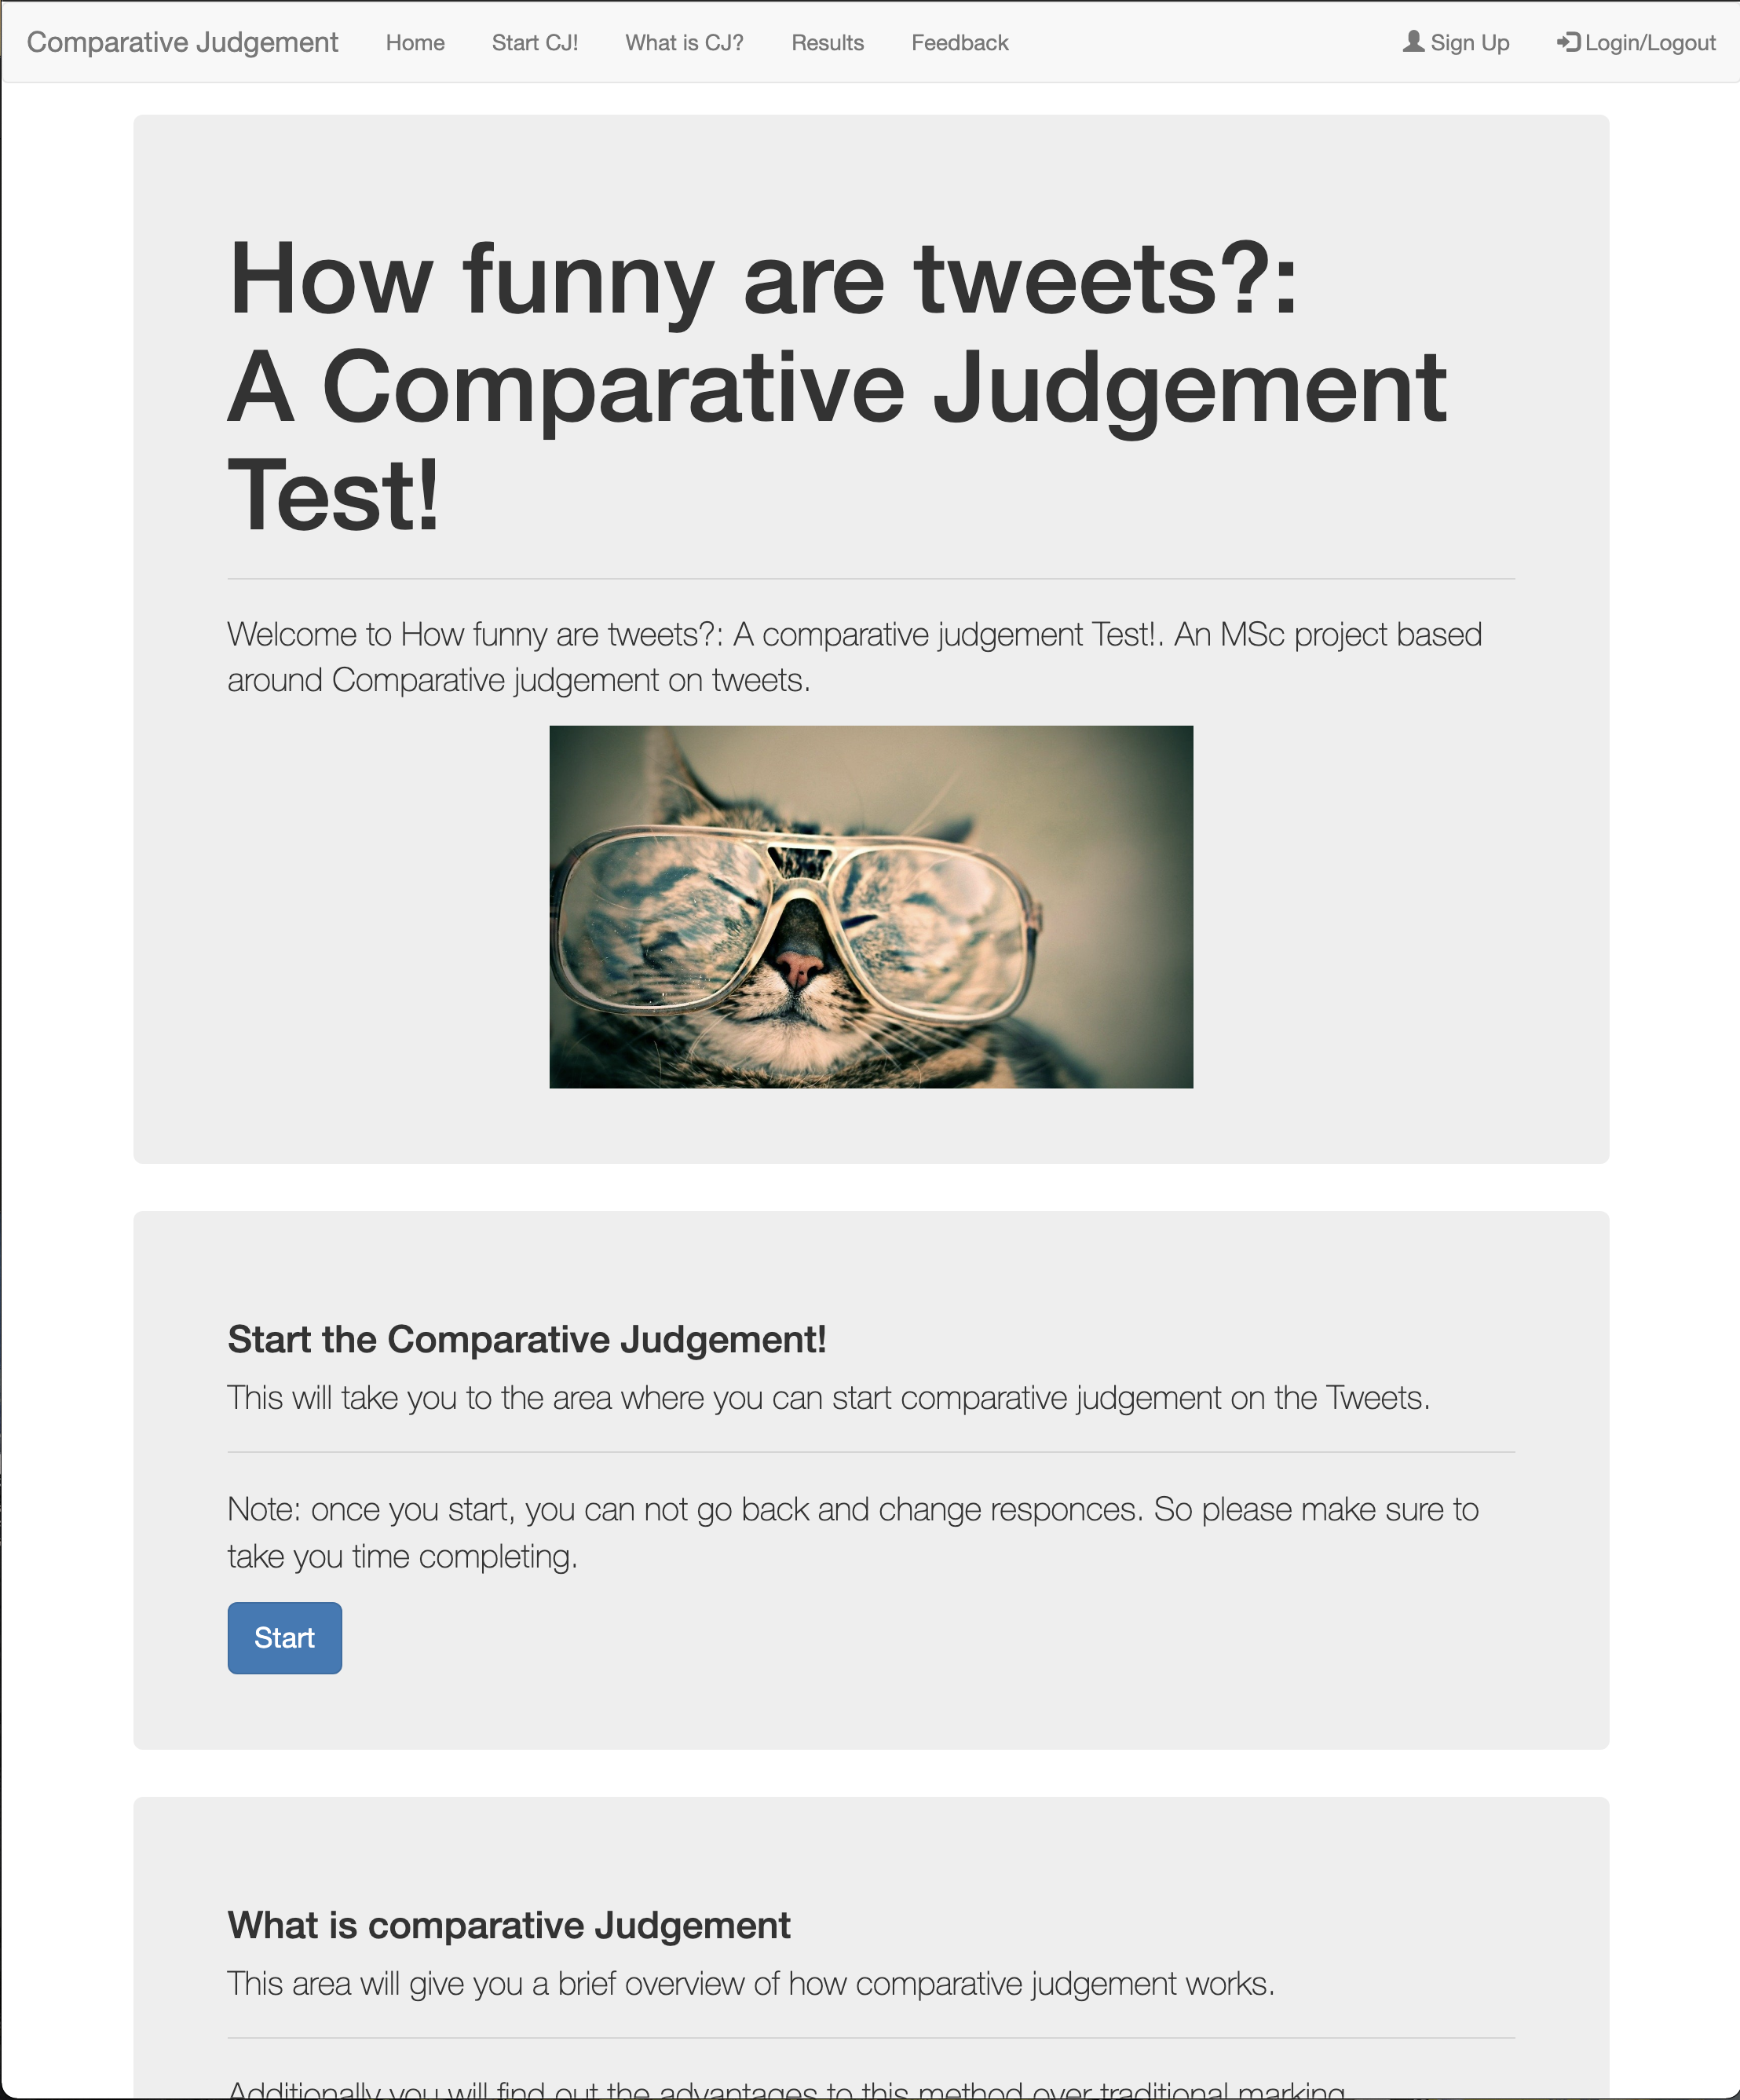
\includegraphics[width=10cm]{Home_page.png}
	\caption{}
	
		
	\end{figure} 
\begin{figure}[h]
	\centering
	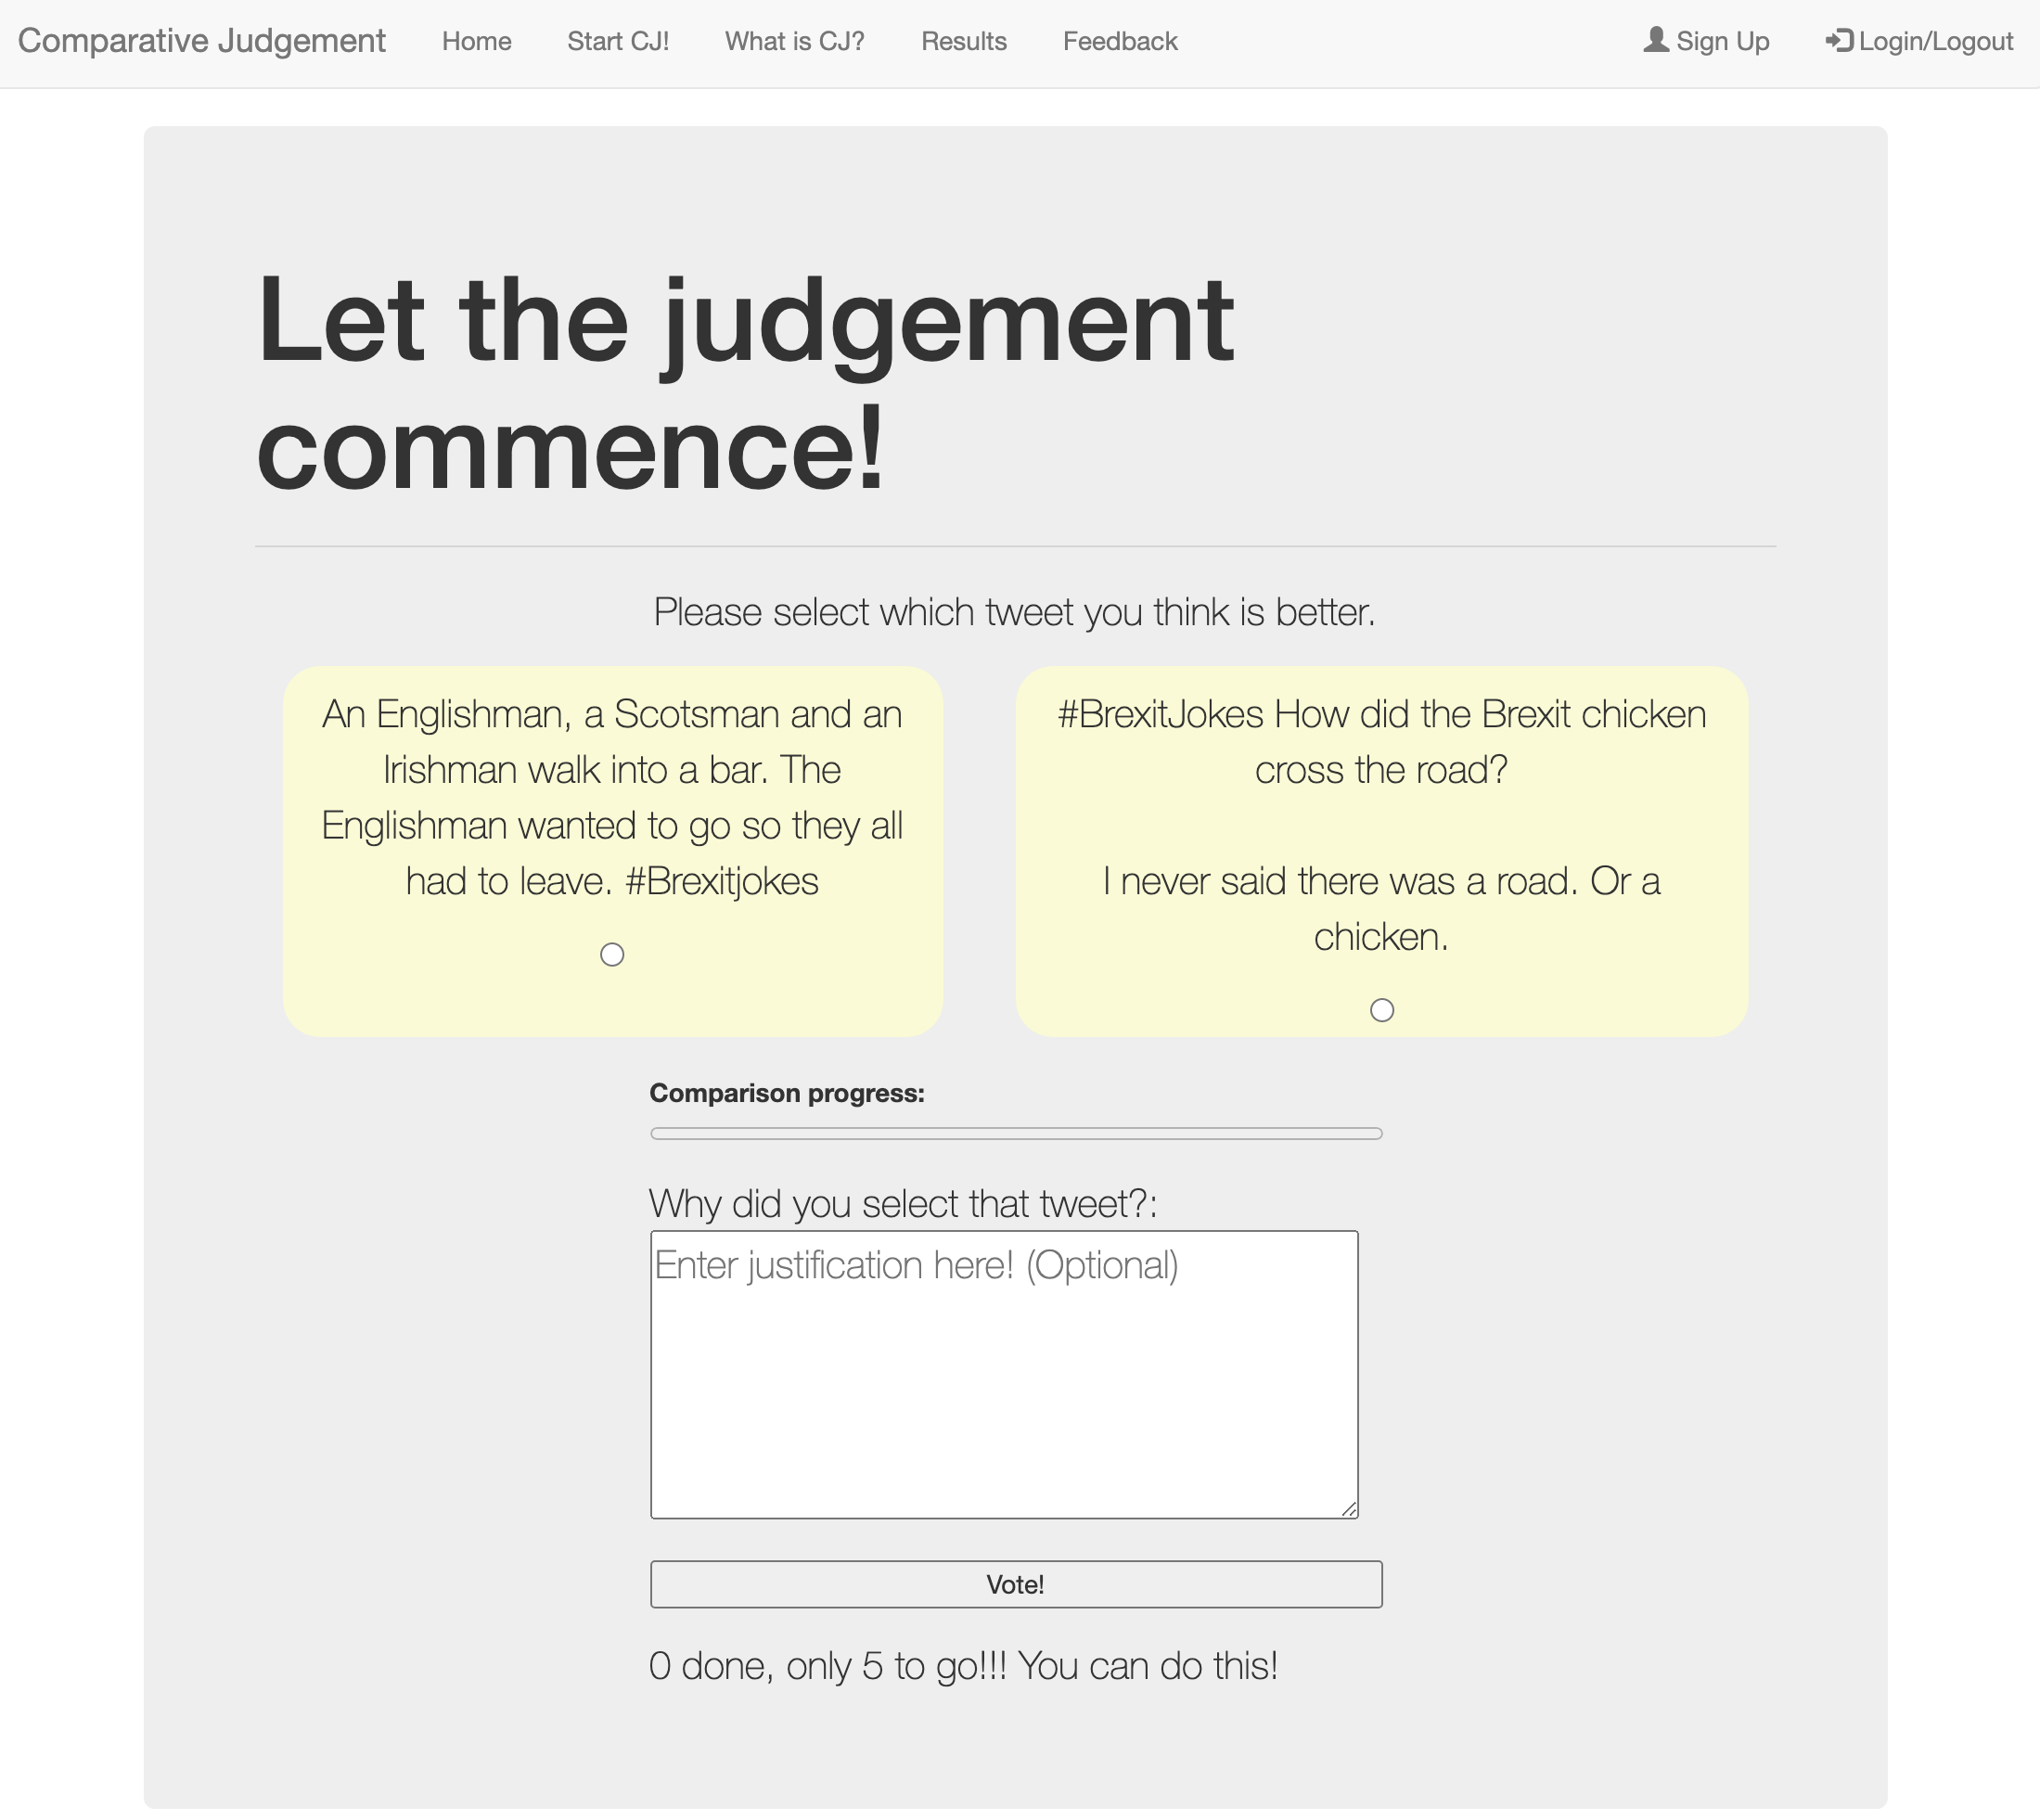
\includegraphics[width=10cm]{Compare.png}
	\caption{}
	
		
	\end{figure} 

\begin{figure}[h]
	\centering
	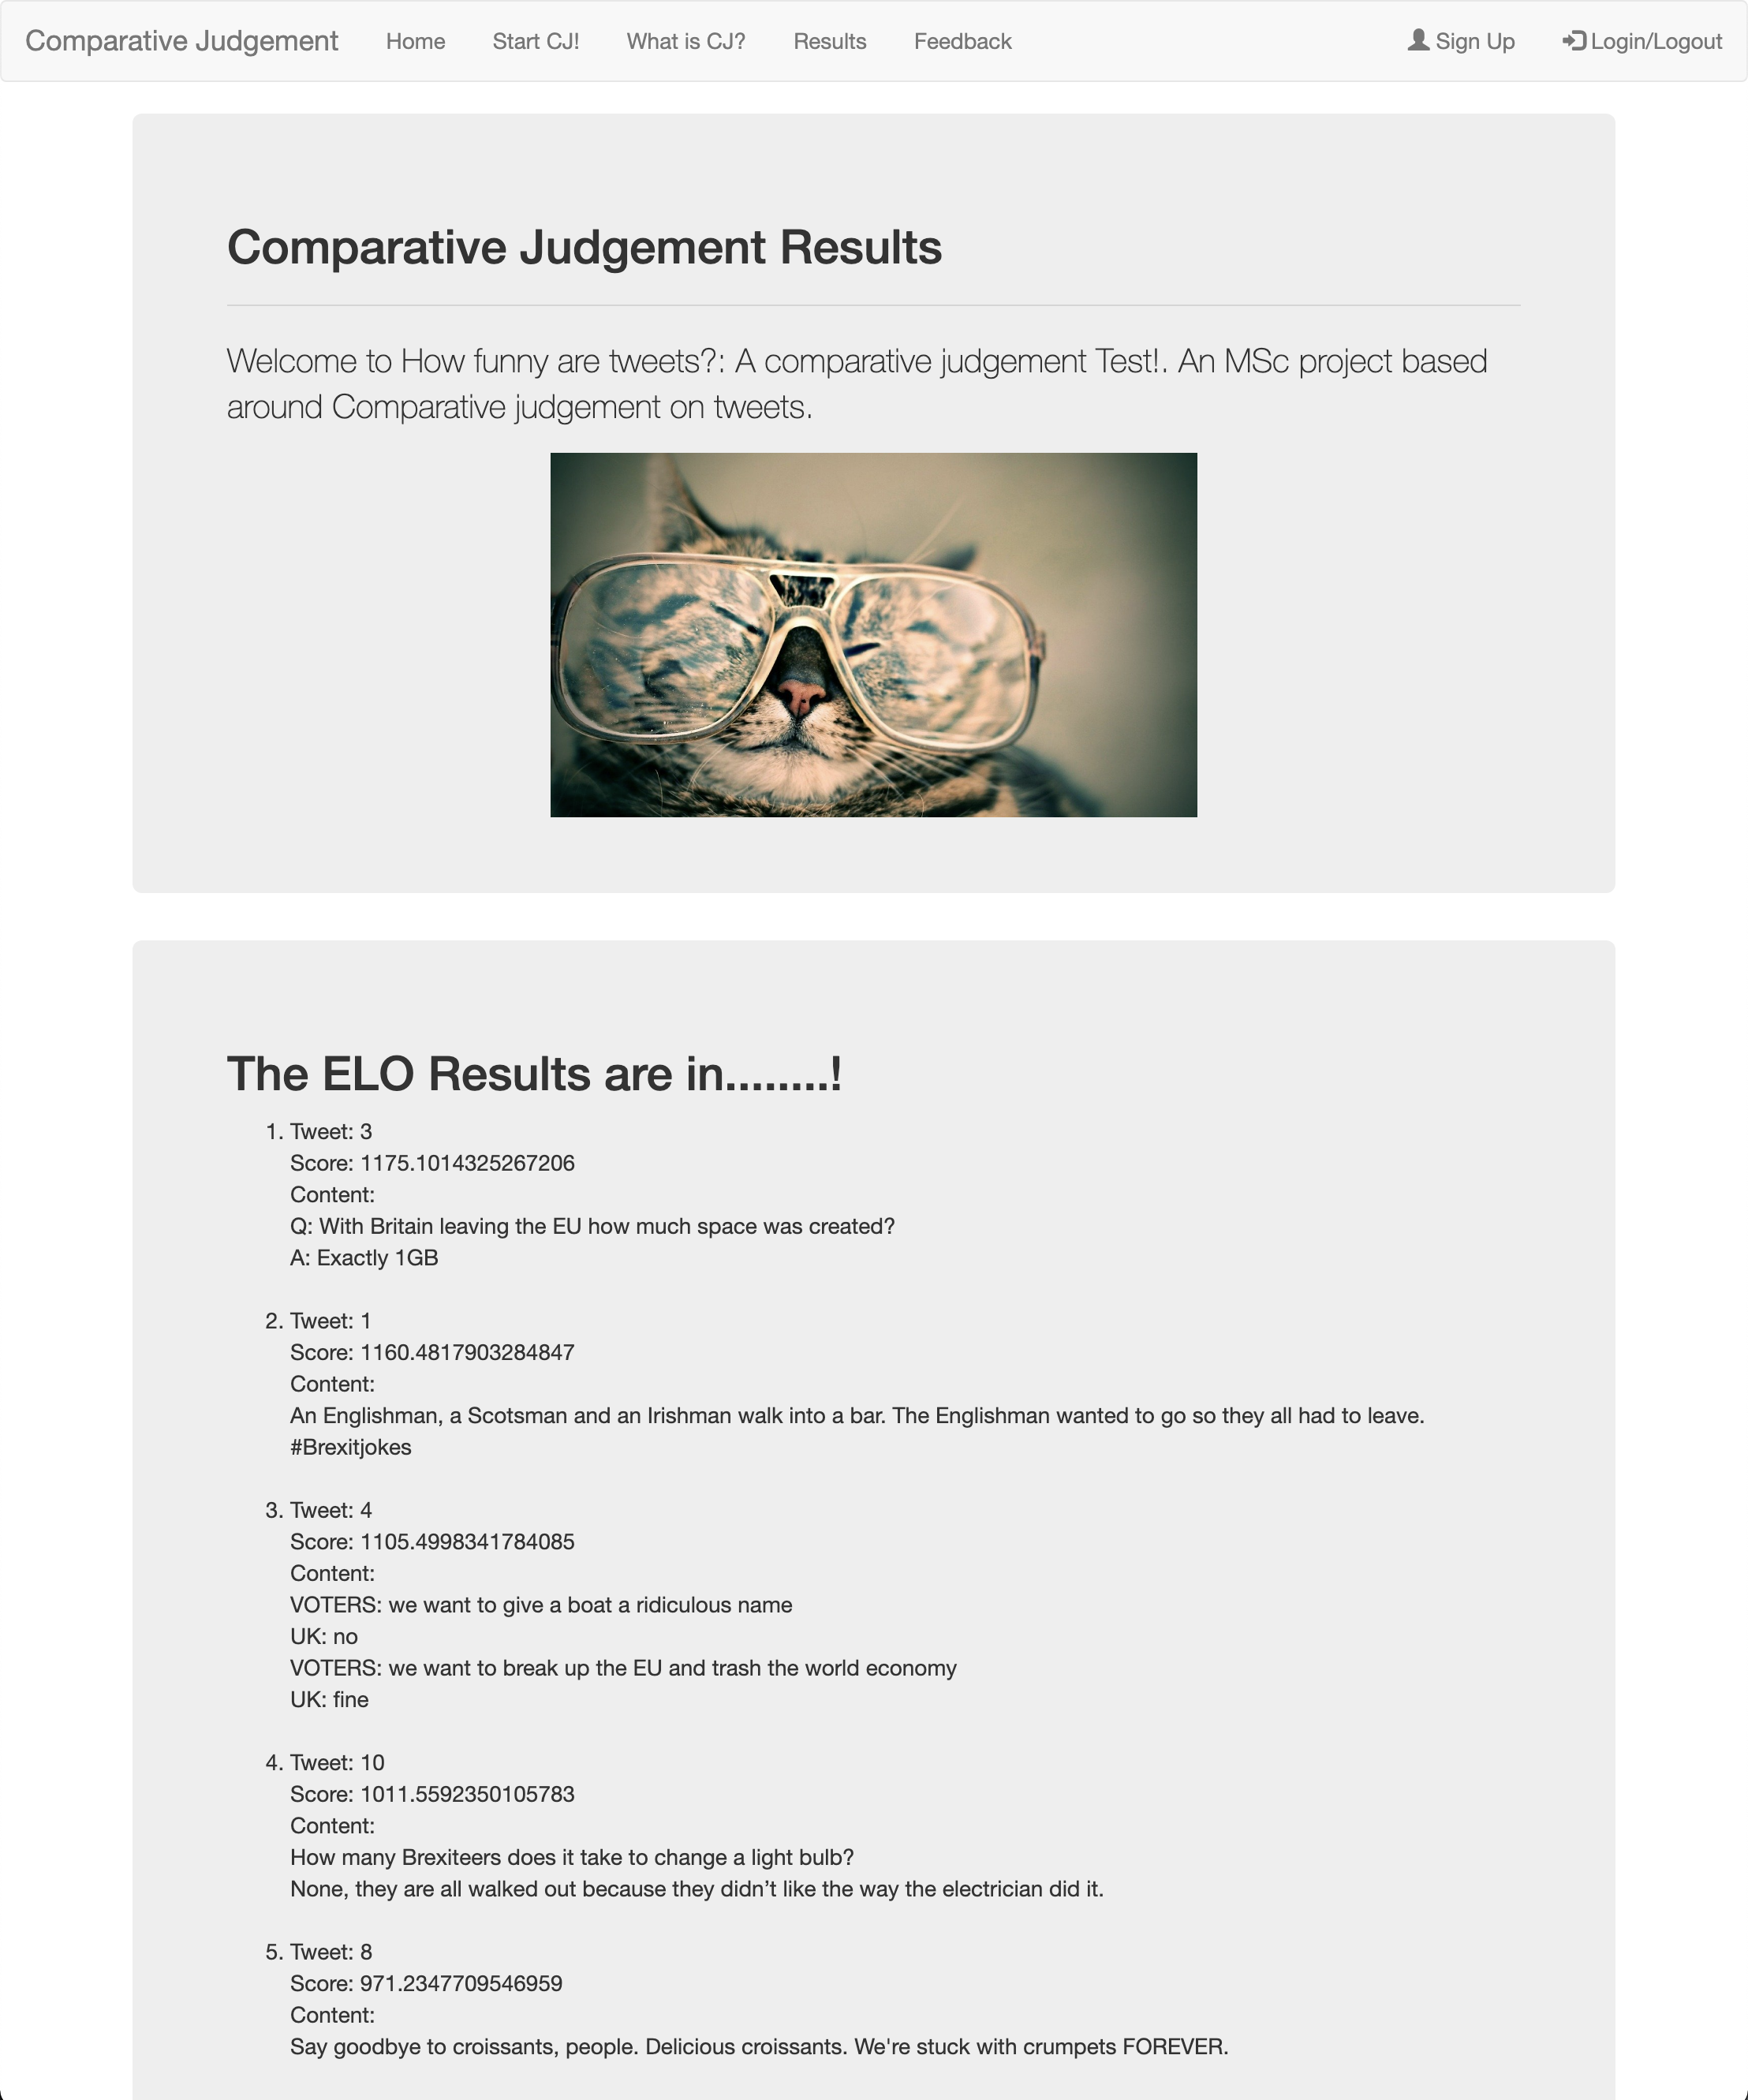
\includegraphics[width=10cm]{Results.png}
	\caption{}
	
		
	\end{figure} 

%\begin{figure}[h]
%	\centering
%	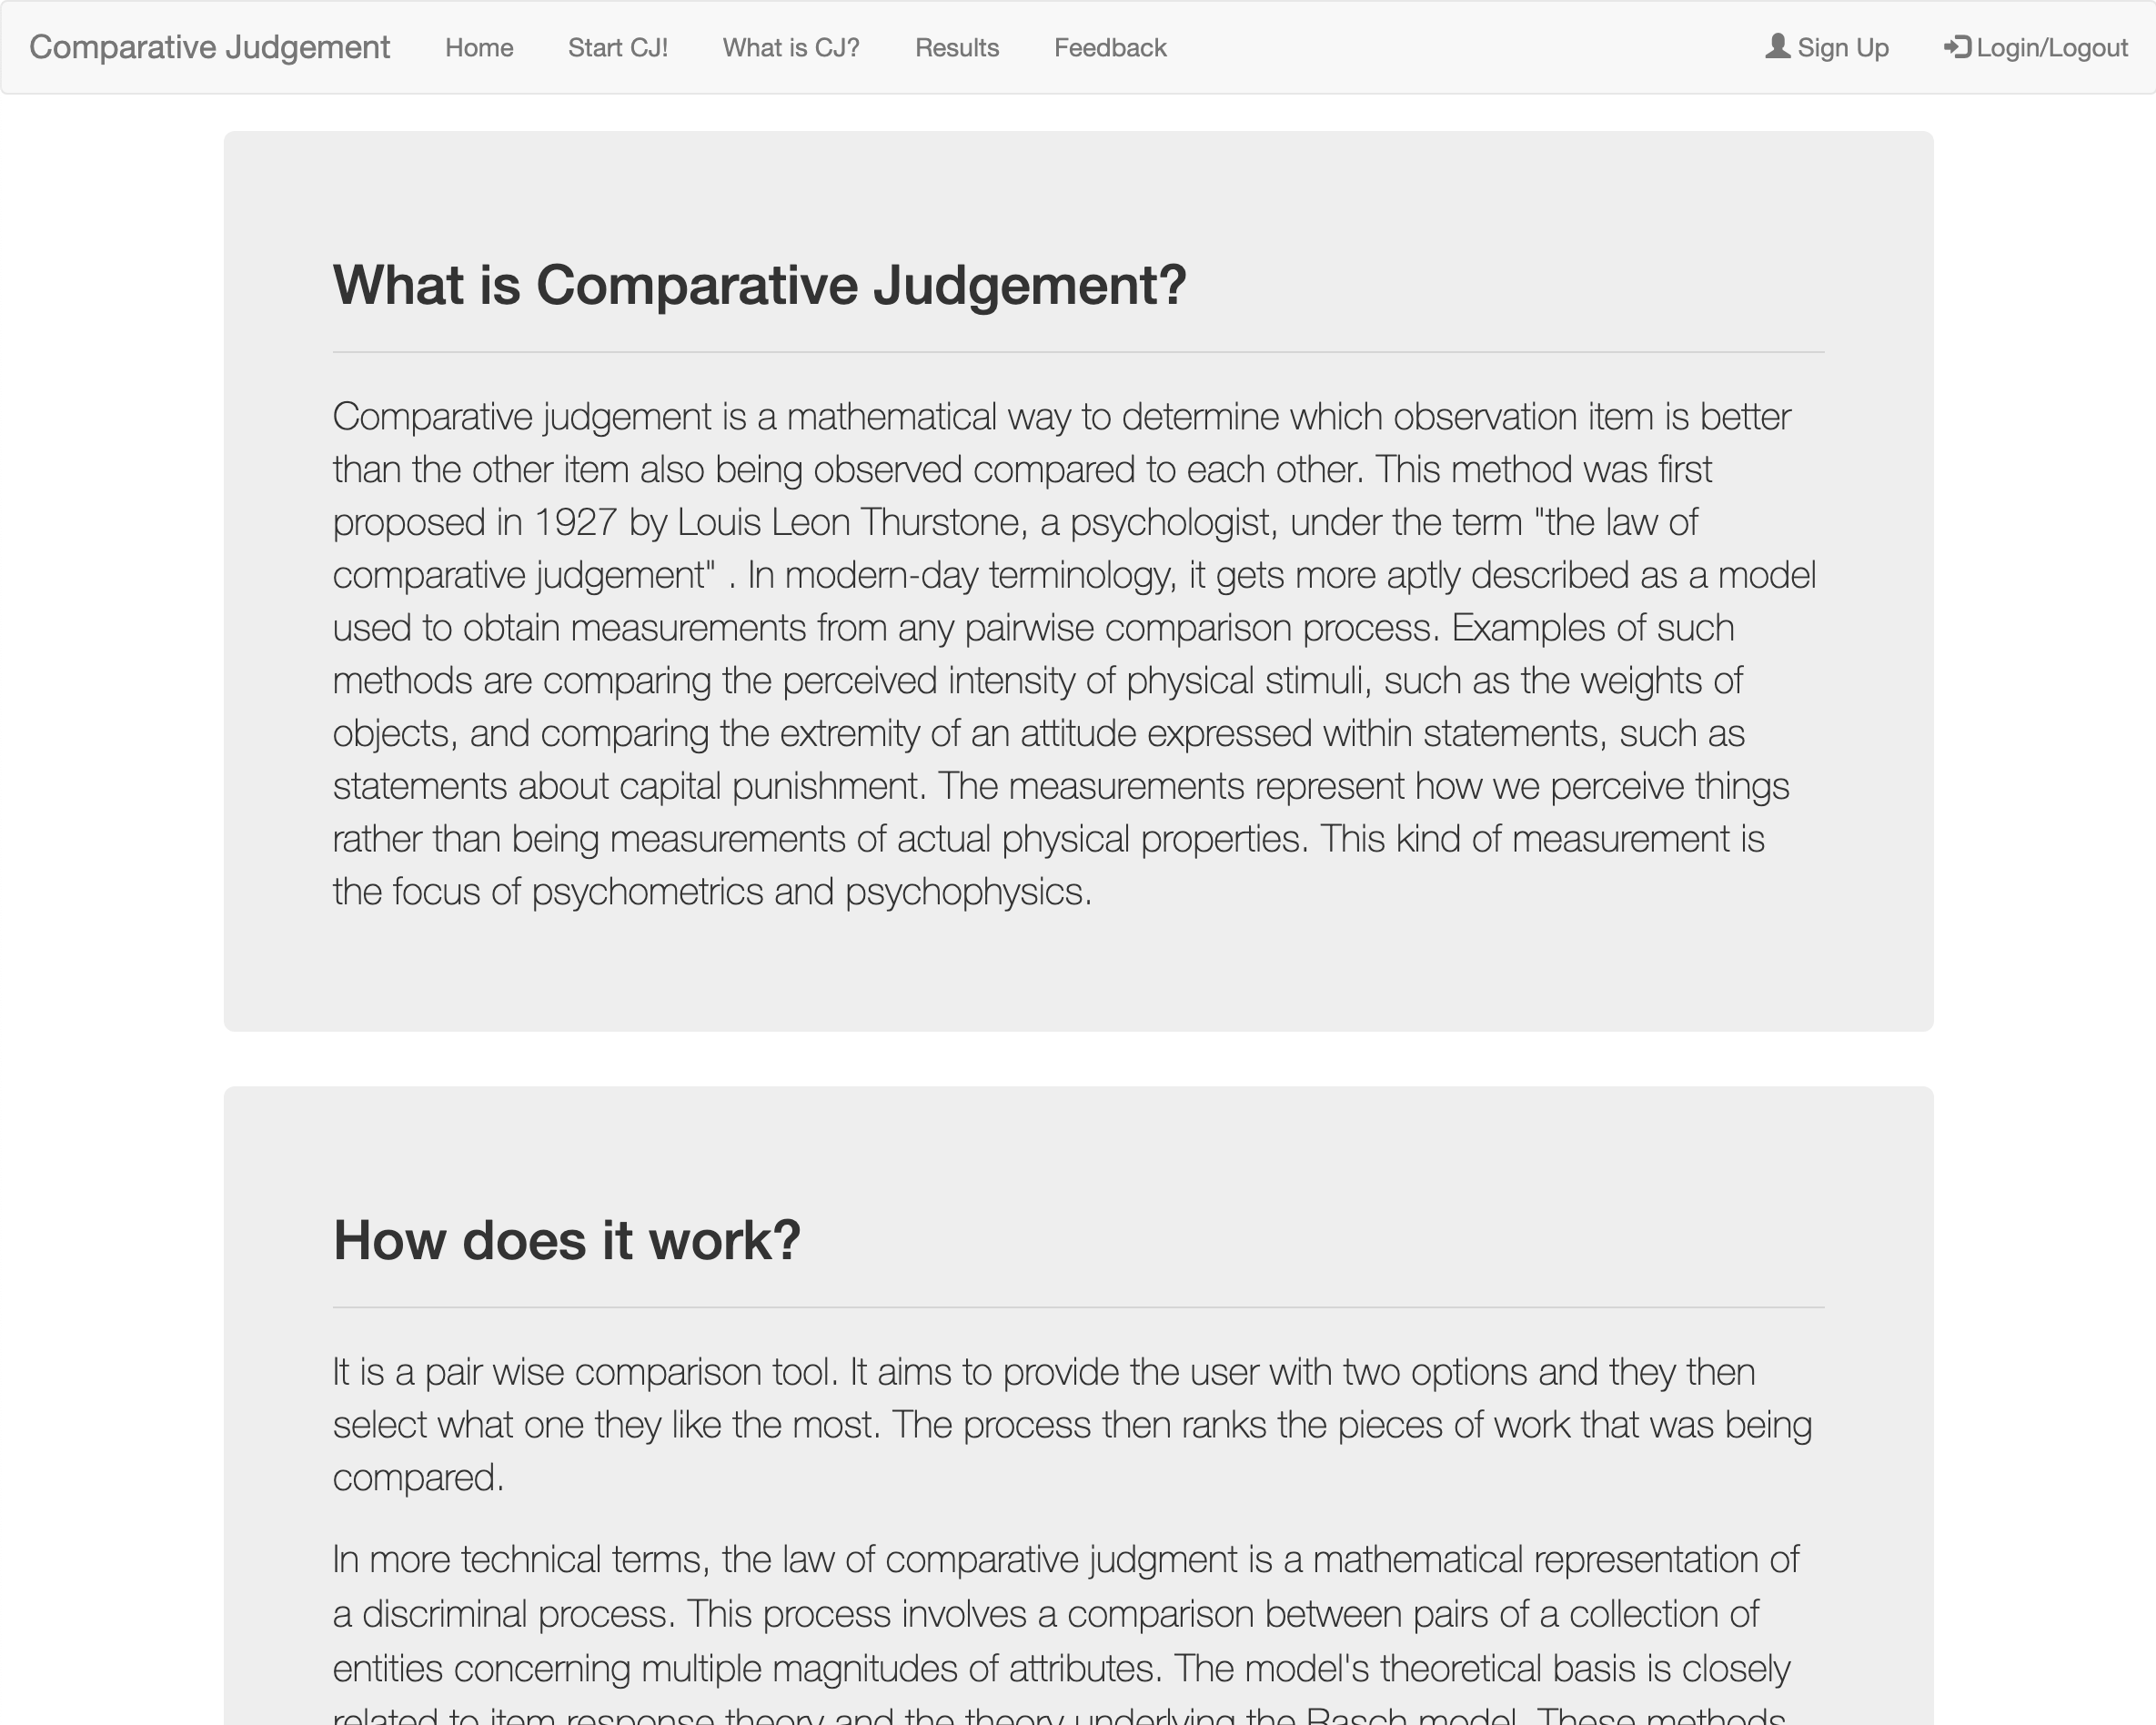
\includegraphics[width=10cm]{What_is_CJ.png.png}
%	\caption{}

		
%	\end{figure} 
\begin{figure}[h]
	\centering
	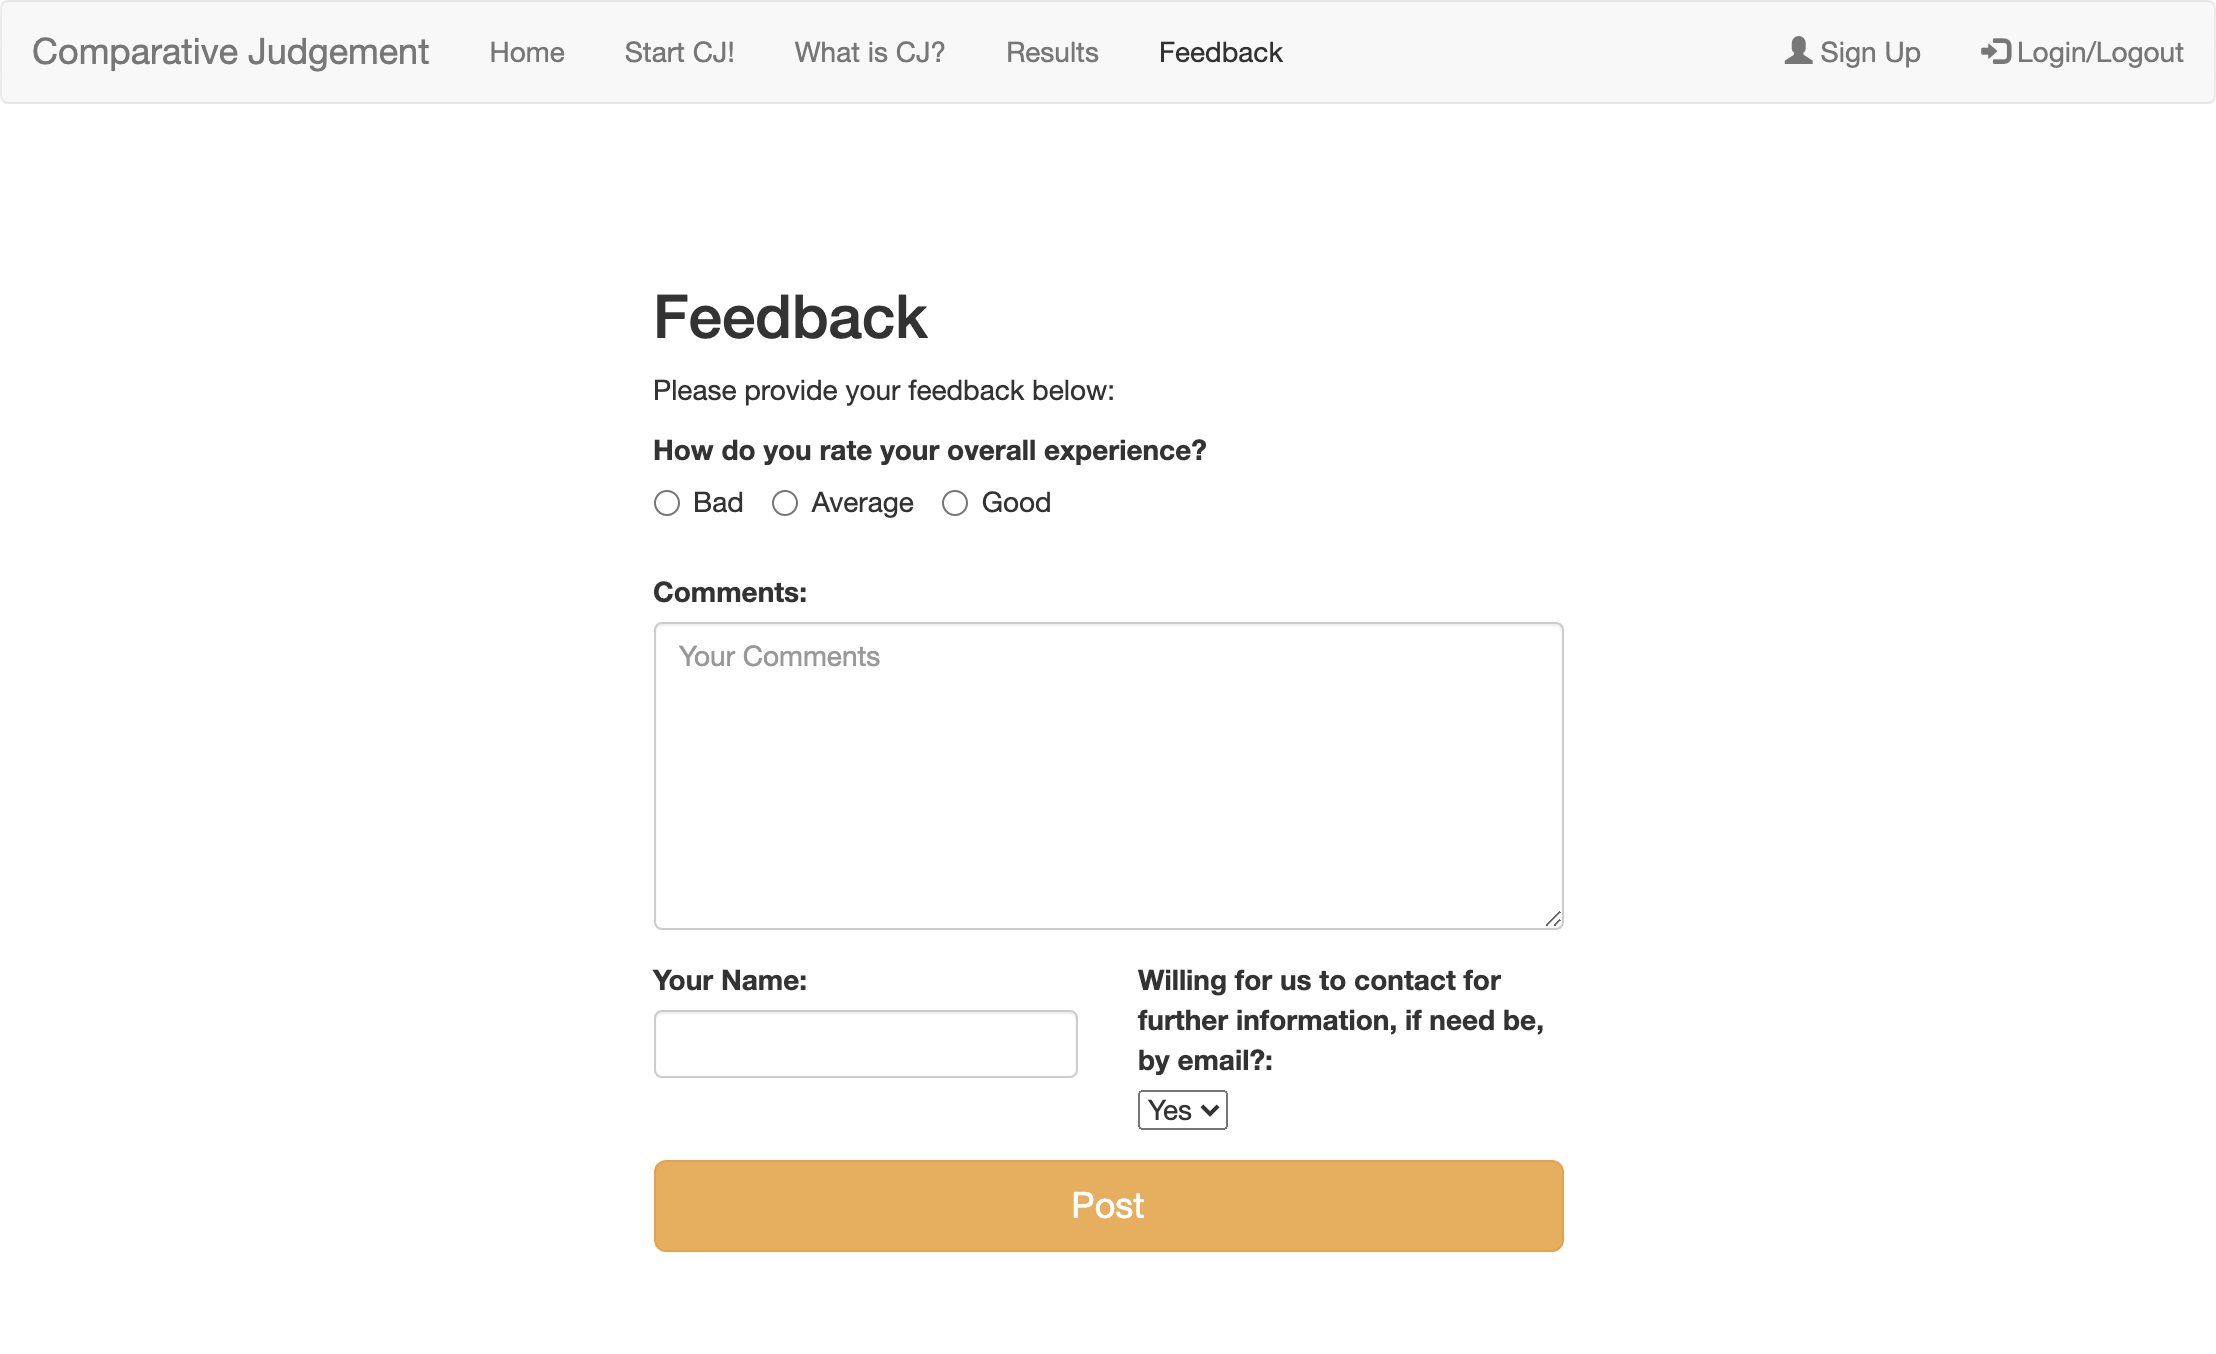
\includegraphics[width=10cm]{feedback.png}
	\caption{}
		
	\end{figure} 

%\begin{figure}[h]
%	\centering
%	\includegraphics[width=10cm]{login.png}
%	\caption{}
	
%\end{figure} 


%\begin{figure}[h]
%	\centering
%	\includegraphics[width=10cm]{signup.png}
%	\caption{}
	
%\end{figure} 

\chapter{Designs}
We will next look at the initial designs compared against the file outcome of the web app. We will also explain the decisions made and what changes we made, and why. 

In total, there are five different pages within the web app. The web app has a home page, facilitates the comparative judgment procedure, results, and feedback.

\subsection{Home Page}

\subsection{Comparison Page}

\subsection{What is Comparative Judgement Page}

\subsection{Results Page}

\subsection{Feedback Page}


\chapter{Risks}


\begin{center}
	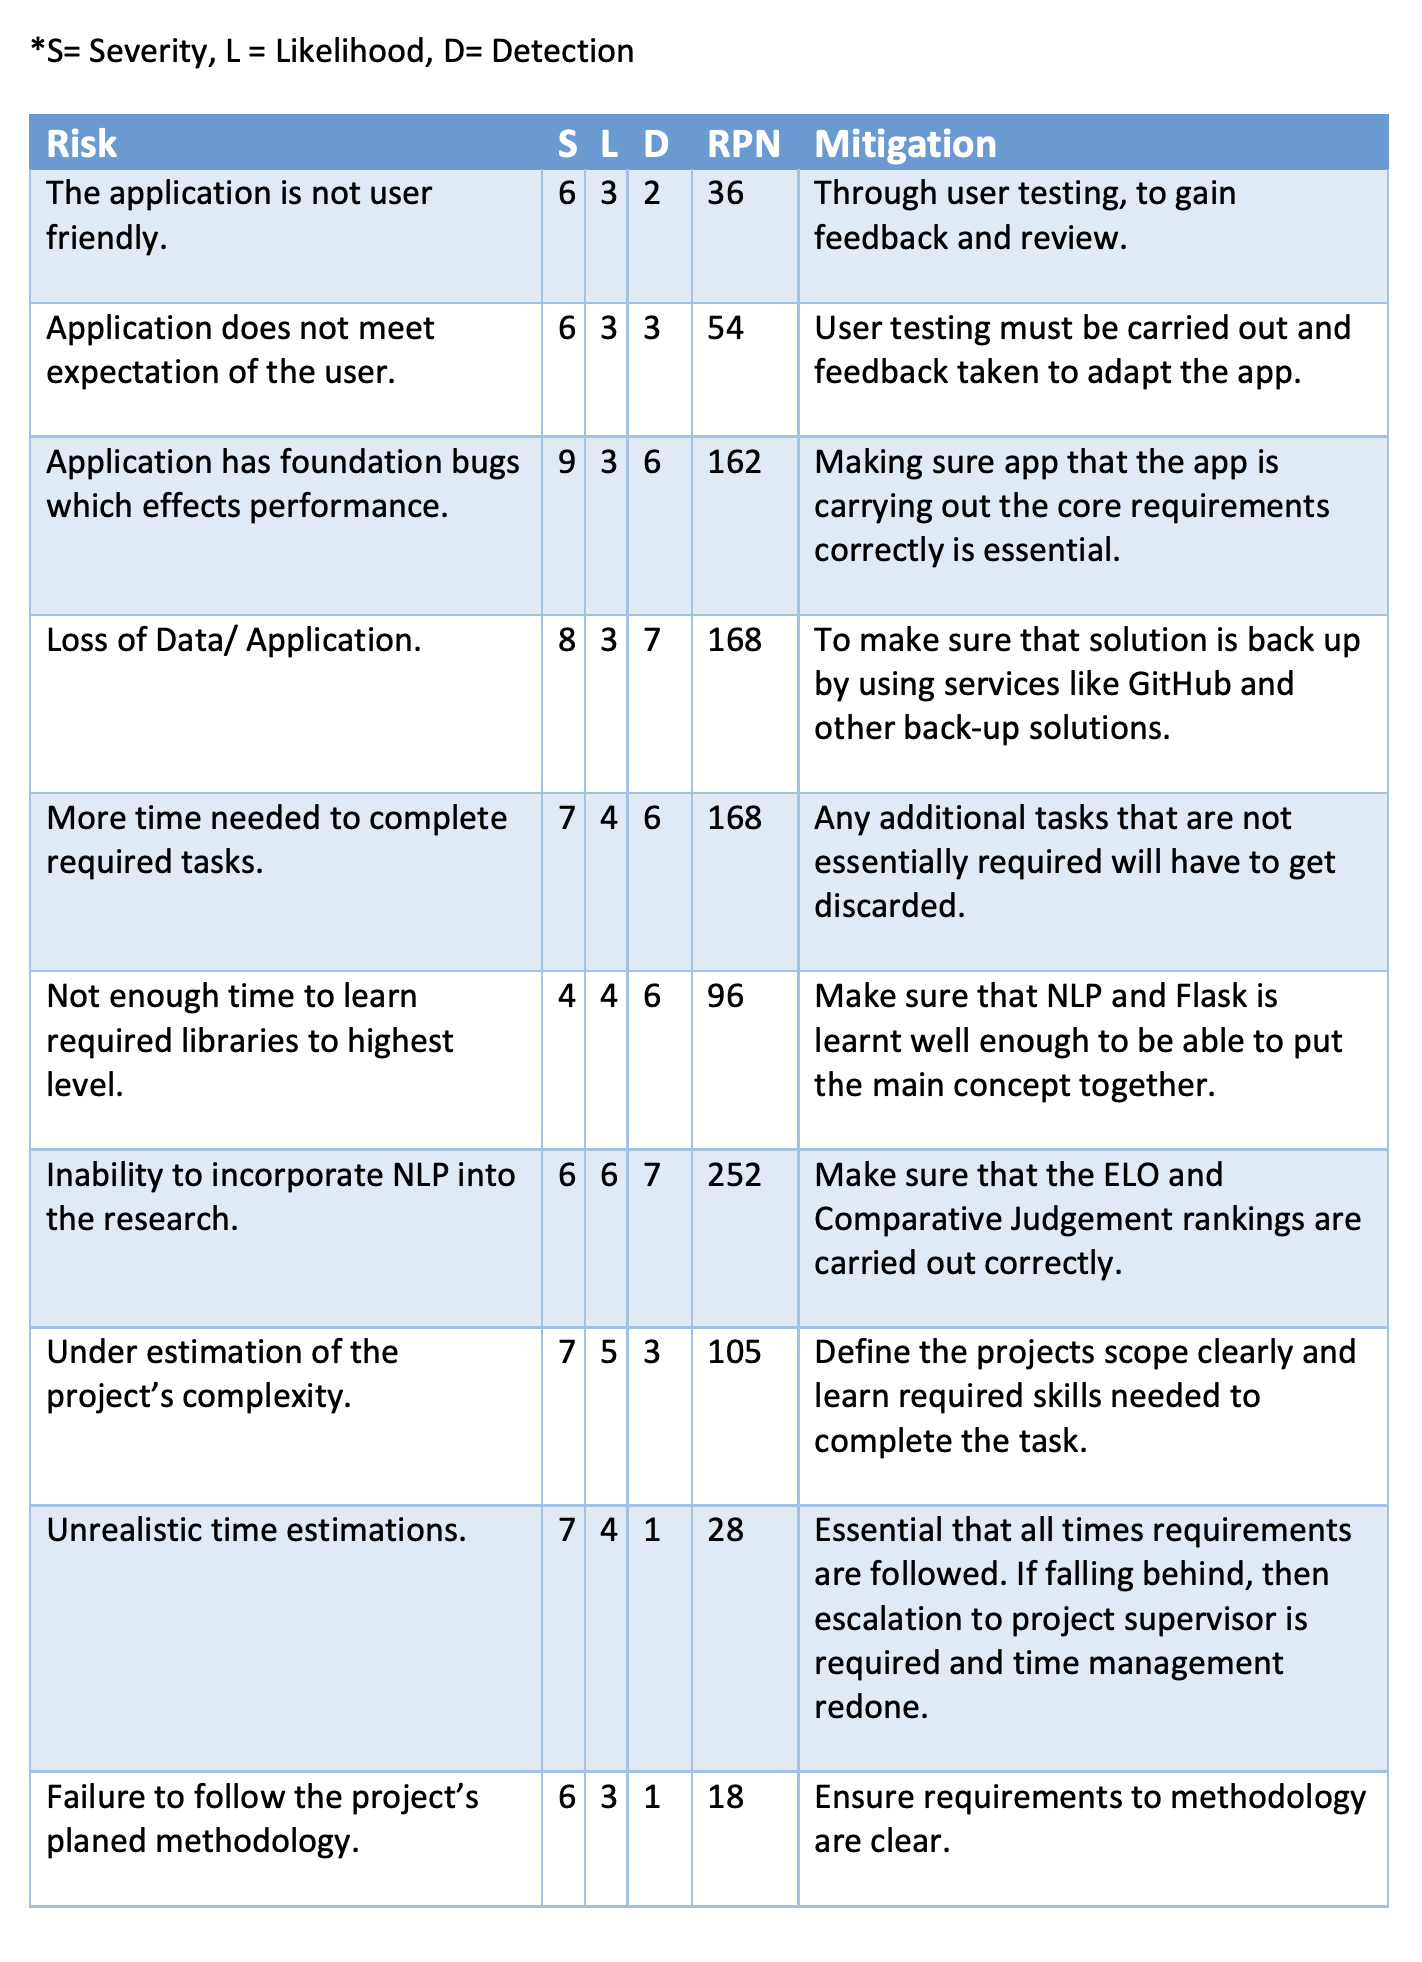
\includegraphics[width=13cm]{risk_table.png}
	%\caption{A visual representation of the processes pipline.}...
\end{center}



\chapter{Schedule}
\begin{landscape}
	
	\begin{center}
		\item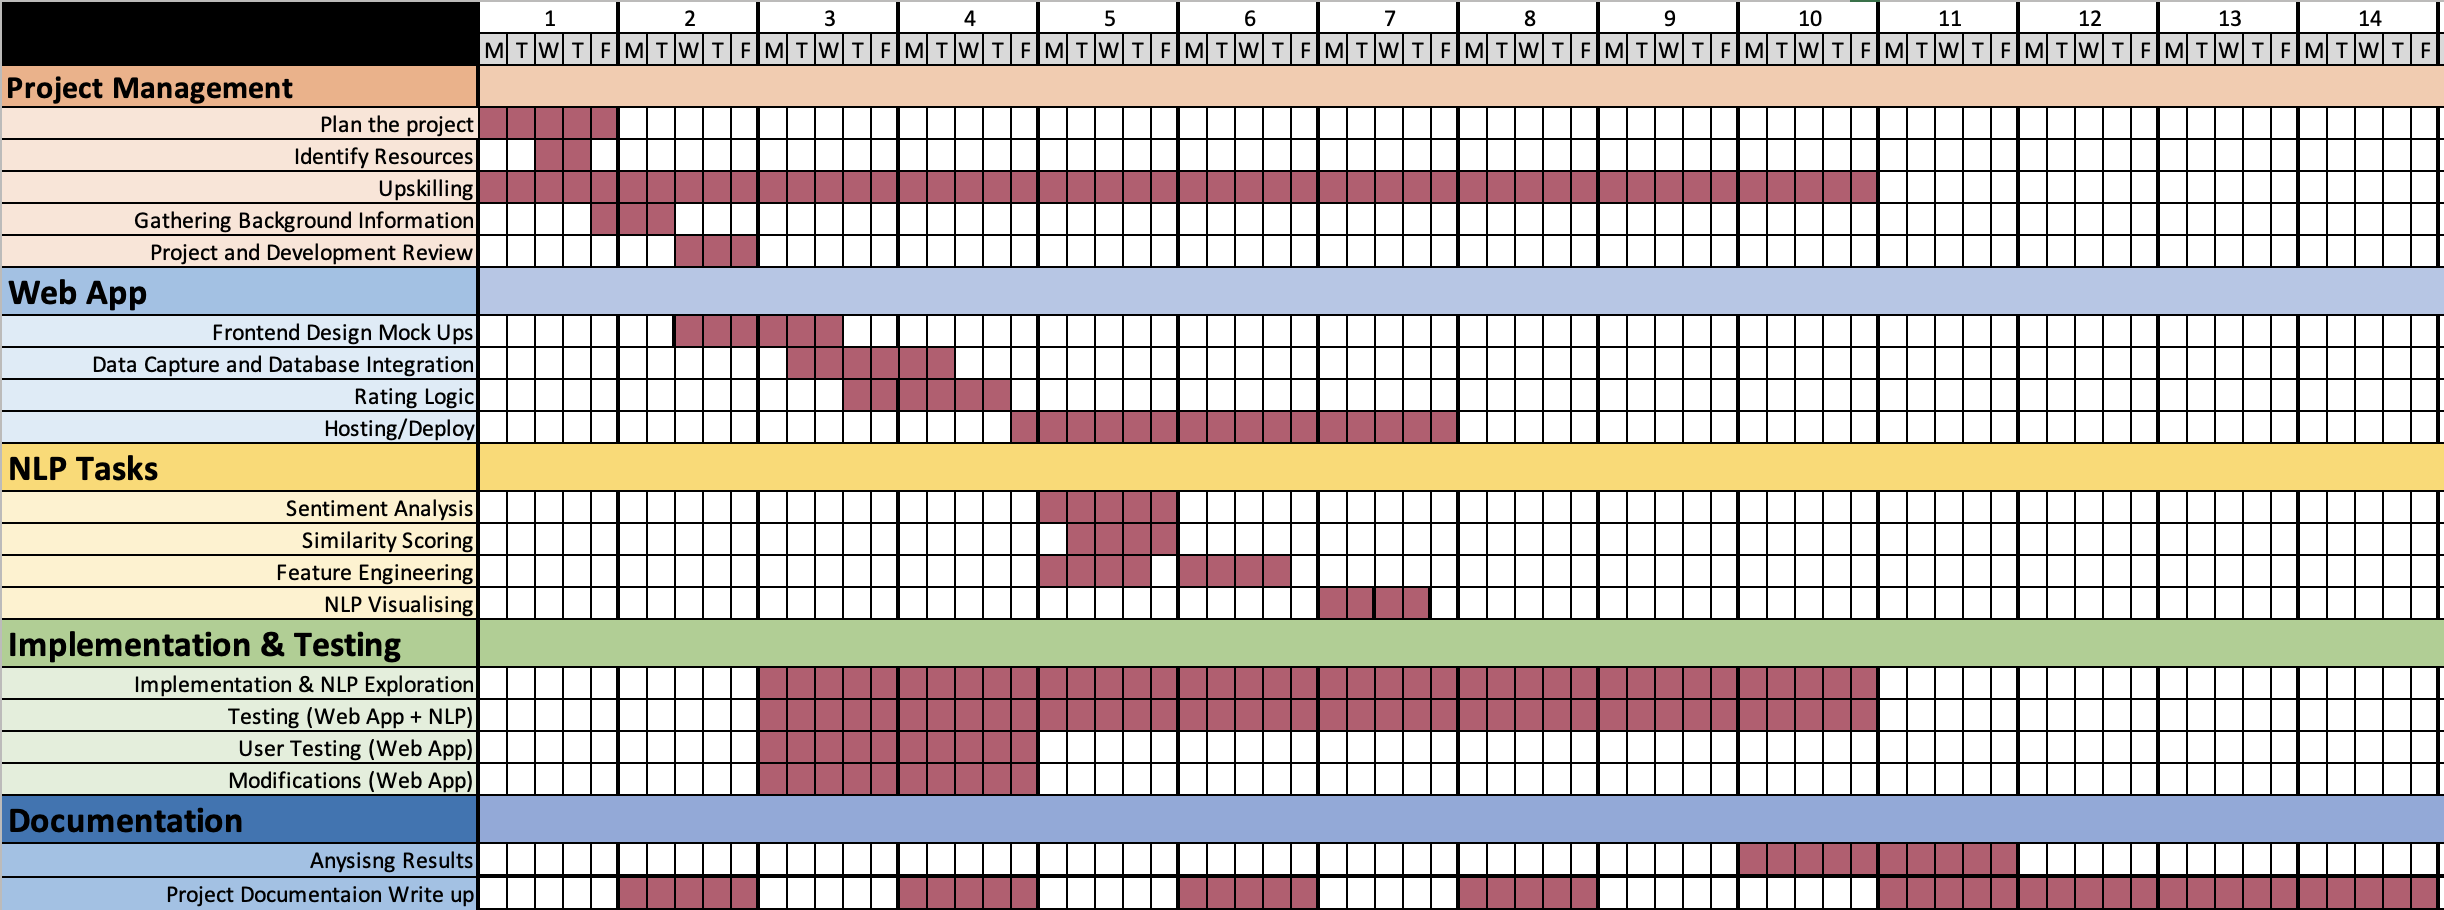
\includegraphics[width=21cm]{ganttchart.png}
	\end{center}
\end{landscape}

\chapter{Software Development Life Cycle Methodology}
Project management is crucial for any task that is about to be carried out, even more so for software development. As a famous Benjamin Franklin quote says, "Failing to plan is planning to fail" \cite{plan_to_fail}. With this in mind, we must decide on the suitable project planning method that compliments our initial software design. From the waterfall method to Rapid application development (RAD) or the more modern methods of agile development, there are many methods that we could choose. We will explain the different methods we could use and what would be best for our solution and intended development method.

The profession of the software developer has existed since the first computers, but the practices and methods for developing software have evolved over timer \cite{SDLC}. The approaches have developed over the years to adapt to the ever-changing landscape of software development. The methods, known as software development life cycles (SDLC), vary in approach but fundamentally share the same goal. The main aims of the SDLC are to break the development up into stages. However, what changes with different SDLC is how these stages get carried out. The different stages are planning, requirements, designing and prototyping, software development, testing, deployment, operations, and maintenance \cite{SDLC}.

The first stage, planning, involves resource allocation, capacity planning, project scheduling, cost estimation, and provisioning \cite{SDLC}. The primary outcome of this stage is to have an overall plan of what we have and what we will need to complete our goal within the constraints like costs and times allowed. The second stage, requirements, is where Subject Matter Experts (SMEs.) guide on what would be needed to carry out the stakeholders' requirements \cite{SDLC}. The third stage, design and prototyping, is where the software architects and developers begin to design the software. The outcome of this stage would be documentation on the intended design patterns and design wireframes of the intended final software. The fourth stage, development, is where the software starts to get made based on the decisions made in design and prototyping, following the chosen methodology. The outcome will be testable, tangible software. The fifth stage, testing, is considered the most crucial stage \cite{SDLC}. It is essential to do all the code quality checking, unit testing, integration testing, performance testing and security testing. The sixth but by no means the final stage is deployment. This stage is when the code is ready to be shipped to the client or uploaded to the required app stores. However, the final stage is operations and maintenance. This stage is about ensuring that the software is getting used as it should and that any bugs that did not initially get picked up in testing are correct and removed from the software. 

%\subsubsection{Waterfall Method}
The waterfall method is a model where each section needs to be completed before moving onto the next stage, like a waterfall flowing down. For example, before we can start analysing the requirements, we need to complete the planning stage. Following the seven critical stages of SDLC, one after the other.

Like all models, they have their advantages and disadvantages. Advantages that this model has is that it is easy to use and follow, and by the way it is all set up, every stage will get finished before the next stage starts. The waterfall method also allows for the project to be easily managed, resulting in easier documentation \cite{cscm01slidesl5}. However, some of the disadvantages are that it is not very useful if the requirements are not very clear at the beginning. Another disadvantage is that once we have moved to the next stage, it is tough to go back to a previous stage to make any changes which therefore creates higher risks to development and has less flexibility \cite{cscm01slidesl5}. The model is best when changes in the project are stable, and the project is small, with the project requirements are clearly defined.

%\subsubsection{RAD: Rapid Application Development}
The overall aim of RAD is to create software projects with higher quality and faster by gathering requirements through workshops or focus groups. Then prototyping the product and then using reiterative user testing of designs early. RAD is the best model for when we need something created quickly and have a pool of users available to test prototypes. However, this approach can be costlym \cite{cscm01slides}. 

%\subsubsection{Spiral Method}
The Spiral Model is an SDLC methodology that aids in choosing the optimal process model. It combines aspects of the incremental build model, waterfall model and prototyping model but is different by a set of six invariant characteristics \cite{spiralmodel}. The Spiral Model main focus is on risk awareness and management. The risk-driven approach of the spiral model ensures the team is highly flexible within its approach and highly aware of the challenges they can expect down the road. The spiral model shines when stakes are highest, and significant setbacks are not an option \cite{spiralmodel}.


%\subsubsection{Agile Development}
The Agile methodology is a process by which a team can manage a project, which gets achieved by breaking up the project into several stages. It required constant collaboration with stakeholders, which leads to continuous iterations of improvement. In essence, Agile development is not a set methodology more of a manifesto aiming to uncover better ways to develop software. "Individuals and interactions over processes and tools. Working software over comprehensive documentation. Customer collaboration over contract negotiation. Responding to change over following a plan \cite{agilemanifesto}."

%\subsubsection{Decided Method}
The project's requirements have features that lend themselves well to the waterfall methodology. However, we would like to have an element of agile methodology within the development due to the application intending to get created in a modular way. Using the waterfall method will allow us to have a clear plan and requirements of what is needed, but by using the agile method, we can rotate between the software development and testing stages.

\chapter{Testing}

The web application was the part of the implementation that required rigorous testing. The testing was because the web app was the bit that users would be interacting with the study. Therefore, we needed to ensure the app was to a high standard not to detract away from the users' experience and solely focus on the application purpose, which is to select which tweet they think is funnier. 

We conducted multiple in-house testing using an internal server's localhost to ensure that the app was suitable. Additionally, we allowed a small number of users to test out the application. Once we were happy with the feedback, the application's data got reset and published to potential users.

\chapter{Implementation of a Web App}
\label{app:implementation_algorithm}

% Code listings should live in a code file, not embedded directly into your LaTeX code!
\lstinputlisting[language=python, caption={The implemented code for handling the main control of the web app.}]{./listings/app.py}
\lstinputlisting[language=python, caption={The implemented code for handling the main web app logic.}]{./listings/logic.py}
\lstinputlisting[language=python, caption={The implemented code for handling Firebase Connections.}]{./listings/models.py}

\chapter{NLP Jupyter Notebook}
\label{app:jupyter_nb}
\documentclass[11pt]{article}

    \usepackage[breakable]{tcolorbox}
    \usepackage{parskip} % Stop auto-indenting (to mimic markdown behaviour)
    
    \usepackage{iftex}
    \ifPDFTeX
    	\usepackage[T1]{fontenc}
    	\usepackage{mathpazo}
    \else
    	\usepackage{fontspec}
    \fi

    % Basic figure setup, for now with no caption control since it's done
    % automatically by Pandoc (which extracts ![](path) syntax from Markdown).
    \usepackage{graphicx}
    % Maintain compatibility with old templates. Remove in nbconvert 6.0
    \let\Oldincludegraphics\includegraphics
    % Ensure that by default, figures have no caption (until we provide a
    % proper Figure object with a Caption API and a way to capture that
    % in the conversion process - todo).
    \usepackage{caption}
    \DeclareCaptionFormat{nocaption}{}
    \captionsetup{format=nocaption,aboveskip=0pt,belowskip=0pt}

    \usepackage{float}
    \floatplacement{figure}{H} % forces figures to be placed at the correct location
    \usepackage{xcolor} % Allow colors to be defined
    \usepackage{enumerate} % Needed for markdown enumerations to work
    \usepackage{geometry} % Used to adjust the document margins
    \usepackage{amsmath} % Equations
    \usepackage{amssymb} % Equations
    \usepackage{textcomp} % defines textquotesingle
    % Hack from http://tex.stackexchange.com/a/47451/13684:
    \AtBeginDocument{%
        \def\PYZsq{\textquotesingle}% Upright quotes in Pygmentized code
    }
    \usepackage{upquote} % Upright quotes for verbatim code
    \usepackage{eurosym} % defines \euro
    \usepackage[mathletters]{ucs} % Extended unicode (utf-8) support
    \usepackage{fancyvrb} % verbatim replacement that allows latex
    \usepackage{grffile} % extends the file name processing of package graphics 
                         % to support a larger range
    \makeatletter % fix for old versions of grffile with XeLaTeX
    \@ifpackagelater{grffile}{2019/11/01}
    {
      % Do nothing on new versions
    }
    {
      \def\Gread@@xetex#1{%
        \IfFileExists{"\Gin@base".bb}%
        {\Gread@eps{\Gin@base.bb}}%
        {\Gread@@xetex@aux#1}%
      }
    }
    \makeatother
    \usepackage[Export]{adjustbox} % Used to constrain images to a maximum size
    \adjustboxset{max size={0.9\linewidth}{0.9\paperheight}}

    % The hyperref package gives us a pdf with properly built
    % internal navigation ('pdf bookmarks' for the table of contents,
    % internal cross-reference links, web links for URLs, etc.)
    \usepackage{hyperref}
    % The default LaTeX title has an obnoxious amount of whitespace. By default,
    % titling removes some of it. It also provides customization options.
    \usepackage{titling}
    \usepackage{longtable} % longtable support required by pandoc >1.10
    \usepackage{booktabs}  % table support for pandoc > 1.12.2
    \usepackage[inline]{enumitem} % IRkernel/repr support (it uses the enumerate* environment)
    \usepackage[normalem]{ulem} % ulem is needed to support strikethroughs (\sout)
                                % normalem makes italics be italics, not underlines
    \usepackage{mathrsfs}
    

    
    % Colors for the hyperref package
    \definecolor{urlcolor}{rgb}{0,.145,.698}
    \definecolor{linkcolor}{rgb}{.71,0.21,0.01}
    \definecolor{citecolor}{rgb}{.12,.54,.11}

    % ANSI colors
    \definecolor{ansi-black}{HTML}{3E424D}
    \definecolor{ansi-black-intense}{HTML}{282C36}
    \definecolor{ansi-red}{HTML}{E75C58}
    \definecolor{ansi-red-intense}{HTML}{B22B31}
    \definecolor{ansi-green}{HTML}{00A250}
    \definecolor{ansi-green-intense}{HTML}{007427}
    \definecolor{ansi-yellow}{HTML}{DDB62B}
    \definecolor{ansi-yellow-intense}{HTML}{B27D12}
    \definecolor{ansi-blue}{HTML}{208FFB}
    \definecolor{ansi-blue-intense}{HTML}{0065CA}
    \definecolor{ansi-magenta}{HTML}{D160C4}
    \definecolor{ansi-magenta-intense}{HTML}{A03196}
    \definecolor{ansi-cyan}{HTML}{60C6C8}
    \definecolor{ansi-cyan-intense}{HTML}{258F8F}
    \definecolor{ansi-white}{HTML}{C5C1B4}
    \definecolor{ansi-white-intense}{HTML}{A1A6B2}
    \definecolor{ansi-default-inverse-fg}{HTML}{FFFFFF}
    \definecolor{ansi-default-inverse-bg}{HTML}{000000}

    % common color for the border for error outputs.
    \definecolor{outerrorbackground}{HTML}{FFDFDF}

    % commands and environments needed by pandoc snippets
    % extracted from the output of `pandoc -s`
    \providecommand{\tightlist}{%
      \setlength{\itemsep}{0pt}\setlength{\parskip}{0pt}}
    \DefineVerbatimEnvironment{Highlighting}{Verbatim}{commandchars=\\\{\}}
    % Add ',fontsize=\small' for more characters per line
    \newenvironment{Shaded}{}{}
    \newcommand{\KeywordTok}[1]{\textcolor[rgb]{0.00,0.44,0.13}{\textbf{{#1}}}}
    \newcommand{\DataTypeTok}[1]{\textcolor[rgb]{0.56,0.13,0.00}{{#1}}}
    \newcommand{\DecValTok}[1]{\textcolor[rgb]{0.25,0.63,0.44}{{#1}}}
    \newcommand{\BaseNTok}[1]{\textcolor[rgb]{0.25,0.63,0.44}{{#1}}}
    \newcommand{\FloatTok}[1]{\textcolor[rgb]{0.25,0.63,0.44}{{#1}}}
    \newcommand{\CharTok}[1]{\textcolor[rgb]{0.25,0.44,0.63}{{#1}}}
    \newcommand{\StringTok}[1]{\textcolor[rgb]{0.25,0.44,0.63}{{#1}}}
    \newcommand{\CommentTok}[1]{\textcolor[rgb]{0.38,0.63,0.69}{\textit{{#1}}}}
    \newcommand{\OtherTok}[1]{\textcolor[rgb]{0.00,0.44,0.13}{{#1}}}
    \newcommand{\AlertTok}[1]{\textcolor[rgb]{1.00,0.00,0.00}{\textbf{{#1}}}}
    \newcommand{\FunctionTok}[1]{\textcolor[rgb]{0.02,0.16,0.49}{{#1}}}
    \newcommand{\RegionMarkerTok}[1]{{#1}}
    \newcommand{\ErrorTok}[1]{\textcolor[rgb]{1.00,0.00,0.00}{\textbf{{#1}}}}
    \newcommand{\NormalTok}[1]{{#1}}
    
    % Additional commands for more recent versions of Pandoc
    \newcommand{\ConstantTok}[1]{\textcolor[rgb]{0.53,0.00,0.00}{{#1}}}
    \newcommand{\SpecialCharTok}[1]{\textcolor[rgb]{0.25,0.44,0.63}{{#1}}}
    \newcommand{\VerbatimStringTok}[1]{\textcolor[rgb]{0.25,0.44,0.63}{{#1}}}
    \newcommand{\SpecialStringTok}[1]{\textcolor[rgb]{0.73,0.40,0.53}{{#1}}}
    \newcommand{\ImportTok}[1]{{#1}}
    \newcommand{\DocumentationTok}[1]{\textcolor[rgb]{0.73,0.13,0.13}{\textit{{#1}}}}
    \newcommand{\AnnotationTok}[1]{\textcolor[rgb]{0.38,0.63,0.69}{\textbf{\textit{{#1}}}}}
    \newcommand{\CommentVarTok}[1]{\textcolor[rgb]{0.38,0.63,0.69}{\textbf{\textit{{#1}}}}}
    \newcommand{\VariableTok}[1]{\textcolor[rgb]{0.10,0.09,0.49}{{#1}}}
    \newcommand{\ControlFlowTok}[1]{\textcolor[rgb]{0.00,0.44,0.13}{\textbf{{#1}}}}
    \newcommand{\OperatorTok}[1]{\textcolor[rgb]{0.40,0.40,0.40}{{#1}}}
    \newcommand{\BuiltInTok}[1]{{#1}}
    \newcommand{\ExtensionTok}[1]{{#1}}
    \newcommand{\PreprocessorTok}[1]{\textcolor[rgb]{0.74,0.48,0.00}{{#1}}}
    \newcommand{\AttributeTok}[1]{\textcolor[rgb]{0.49,0.56,0.16}{{#1}}}
    \newcommand{\InformationTok}[1]{\textcolor[rgb]{0.38,0.63,0.69}{\textbf{\textit{{#1}}}}}
    \newcommand{\WarningTok}[1]{\textcolor[rgb]{0.38,0.63,0.69}{\textbf{\textit{{#1}}}}}
    
    
    % Define a nice break command that doesn't care if a line doesn't already
    % exist.
    \def\br{\hspace*{\fill} \\* }
    % Math Jax compatibility definitions
    \def\gt{>}
    \def\lt{<}
    \let\Oldtex\TeX
    \let\Oldlatex\LaTeX
    \renewcommand{\TeX}{\textrm{\Oldtex}}
    \renewcommand{\LaTeX}{\textrm{\Oldlatex}}
    % Document parameters
    % Document title
    \title{tweet\_feedback}
    
    
    
    
    
% Pygments definitions
\makeatletter
\def\PY@reset{\let\PY@it=\relax \let\PY@bf=\relax%
    \let\PY@ul=\relax \let\PY@tc=\relax%
    \let\PY@bc=\relax \let\PY@ff=\relax}
\def\PY@tok#1{\csname PY@tok@#1\endcsname}
\def\PY@toks#1+{\ifx\relax#1\empty\else%
    \PY@tok{#1}\expandafter\PY@toks\fi}
\def\PY@do#1{\PY@bc{\PY@tc{\PY@ul{%
    \PY@it{\PY@bf{\PY@ff{#1}}}}}}}
\def\PY#1#2{\PY@reset\PY@toks#1+\relax+\PY@do{#2}}

\expandafter\def\csname PY@tok@w\endcsname{\def\PY@tc##1{\textcolor[rgb]{0.73,0.73,0.73}{##1}}}
\expandafter\def\csname PY@tok@c\endcsname{\let\PY@it=\textit\def\PY@tc##1{\textcolor[rgb]{0.25,0.50,0.50}{##1}}}
\expandafter\def\csname PY@tok@cp\endcsname{\def\PY@tc##1{\textcolor[rgb]{0.74,0.48,0.00}{##1}}}
\expandafter\def\csname PY@tok@k\endcsname{\let\PY@bf=\textbf\def\PY@tc##1{\textcolor[rgb]{0.00,0.50,0.00}{##1}}}
\expandafter\def\csname PY@tok@kp\endcsname{\def\PY@tc##1{\textcolor[rgb]{0.00,0.50,0.00}{##1}}}
\expandafter\def\csname PY@tok@kt\endcsname{\def\PY@tc##1{\textcolor[rgb]{0.69,0.00,0.25}{##1}}}
\expandafter\def\csname PY@tok@o\endcsname{\def\PY@tc##1{\textcolor[rgb]{0.40,0.40,0.40}{##1}}}
\expandafter\def\csname PY@tok@ow\endcsname{\let\PY@bf=\textbf\def\PY@tc##1{\textcolor[rgb]{0.67,0.13,1.00}{##1}}}
\expandafter\def\csname PY@tok@nb\endcsname{\def\PY@tc##1{\textcolor[rgb]{0.00,0.50,0.00}{##1}}}
\expandafter\def\csname PY@tok@nf\endcsname{\def\PY@tc##1{\textcolor[rgb]{0.00,0.00,1.00}{##1}}}
\expandafter\def\csname PY@tok@nc\endcsname{\let\PY@bf=\textbf\def\PY@tc##1{\textcolor[rgb]{0.00,0.00,1.00}{##1}}}
\expandafter\def\csname PY@tok@nn\endcsname{\let\PY@bf=\textbf\def\PY@tc##1{\textcolor[rgb]{0.00,0.00,1.00}{##1}}}
\expandafter\def\csname PY@tok@ne\endcsname{\let\PY@bf=\textbf\def\PY@tc##1{\textcolor[rgb]{0.82,0.25,0.23}{##1}}}
\expandafter\def\csname PY@tok@nv\endcsname{\def\PY@tc##1{\textcolor[rgb]{0.10,0.09,0.49}{##1}}}
\expandafter\def\csname PY@tok@no\endcsname{\def\PY@tc##1{\textcolor[rgb]{0.53,0.00,0.00}{##1}}}
\expandafter\def\csname PY@tok@nl\endcsname{\def\PY@tc##1{\textcolor[rgb]{0.63,0.63,0.00}{##1}}}
\expandafter\def\csname PY@tok@ni\endcsname{\let\PY@bf=\textbf\def\PY@tc##1{\textcolor[rgb]{0.60,0.60,0.60}{##1}}}
\expandafter\def\csname PY@tok@na\endcsname{\def\PY@tc##1{\textcolor[rgb]{0.49,0.56,0.16}{##1}}}
\expandafter\def\csname PY@tok@nt\endcsname{\let\PY@bf=\textbf\def\PY@tc##1{\textcolor[rgb]{0.00,0.50,0.00}{##1}}}
\expandafter\def\csname PY@tok@nd\endcsname{\def\PY@tc##1{\textcolor[rgb]{0.67,0.13,1.00}{##1}}}
\expandafter\def\csname PY@tok@s\endcsname{\def\PY@tc##1{\textcolor[rgb]{0.73,0.13,0.13}{##1}}}
\expandafter\def\csname PY@tok@sd\endcsname{\let\PY@it=\textit\def\PY@tc##1{\textcolor[rgb]{0.73,0.13,0.13}{##1}}}
\expandafter\def\csname PY@tok@si\endcsname{\let\PY@bf=\textbf\def\PY@tc##1{\textcolor[rgb]{0.73,0.40,0.53}{##1}}}
\expandafter\def\csname PY@tok@se\endcsname{\let\PY@bf=\textbf\def\PY@tc##1{\textcolor[rgb]{0.73,0.40,0.13}{##1}}}
\expandafter\def\csname PY@tok@sr\endcsname{\def\PY@tc##1{\textcolor[rgb]{0.73,0.40,0.53}{##1}}}
\expandafter\def\csname PY@tok@ss\endcsname{\def\PY@tc##1{\textcolor[rgb]{0.10,0.09,0.49}{##1}}}
\expandafter\def\csname PY@tok@sx\endcsname{\def\PY@tc##1{\textcolor[rgb]{0.00,0.50,0.00}{##1}}}
\expandafter\def\csname PY@tok@m\endcsname{\def\PY@tc##1{\textcolor[rgb]{0.40,0.40,0.40}{##1}}}
\expandafter\def\csname PY@tok@gh\endcsname{\let\PY@bf=\textbf\def\PY@tc##1{\textcolor[rgb]{0.00,0.00,0.50}{##1}}}
\expandafter\def\csname PY@tok@gu\endcsname{\let\PY@bf=\textbf\def\PY@tc##1{\textcolor[rgb]{0.50,0.00,0.50}{##1}}}
\expandafter\def\csname PY@tok@gd\endcsname{\def\PY@tc##1{\textcolor[rgb]{0.63,0.00,0.00}{##1}}}
\expandafter\def\csname PY@tok@gi\endcsname{\def\PY@tc##1{\textcolor[rgb]{0.00,0.63,0.00}{##1}}}
\expandafter\def\csname PY@tok@gr\endcsname{\def\PY@tc##1{\textcolor[rgb]{1.00,0.00,0.00}{##1}}}
\expandafter\def\csname PY@tok@ge\endcsname{\let\PY@it=\textit}
\expandafter\def\csname PY@tok@gs\endcsname{\let\PY@bf=\textbf}
\expandafter\def\csname PY@tok@gp\endcsname{\let\PY@bf=\textbf\def\PY@tc##1{\textcolor[rgb]{0.00,0.00,0.50}{##1}}}
\expandafter\def\csname PY@tok@go\endcsname{\def\PY@tc##1{\textcolor[rgb]{0.53,0.53,0.53}{##1}}}
\expandafter\def\csname PY@tok@gt\endcsname{\def\PY@tc##1{\textcolor[rgb]{0.00,0.27,0.87}{##1}}}
\expandafter\def\csname PY@tok@err\endcsname{\def\PY@bc##1{\setlength{\fboxsep}{0pt}\fcolorbox[rgb]{1.00,0.00,0.00}{1,1,1}{\strut ##1}}}
\expandafter\def\csname PY@tok@kc\endcsname{\let\PY@bf=\textbf\def\PY@tc##1{\textcolor[rgb]{0.00,0.50,0.00}{##1}}}
\expandafter\def\csname PY@tok@kd\endcsname{\let\PY@bf=\textbf\def\PY@tc##1{\textcolor[rgb]{0.00,0.50,0.00}{##1}}}
\expandafter\def\csname PY@tok@kn\endcsname{\let\PY@bf=\textbf\def\PY@tc##1{\textcolor[rgb]{0.00,0.50,0.00}{##1}}}
\expandafter\def\csname PY@tok@kr\endcsname{\let\PY@bf=\textbf\def\PY@tc##1{\textcolor[rgb]{0.00,0.50,0.00}{##1}}}
\expandafter\def\csname PY@tok@bp\endcsname{\def\PY@tc##1{\textcolor[rgb]{0.00,0.50,0.00}{##1}}}
\expandafter\def\csname PY@tok@fm\endcsname{\def\PY@tc##1{\textcolor[rgb]{0.00,0.00,1.00}{##1}}}
\expandafter\def\csname PY@tok@vc\endcsname{\def\PY@tc##1{\textcolor[rgb]{0.10,0.09,0.49}{##1}}}
\expandafter\def\csname PY@tok@vg\endcsname{\def\PY@tc##1{\textcolor[rgb]{0.10,0.09,0.49}{##1}}}
\expandafter\def\csname PY@tok@vi\endcsname{\def\PY@tc##1{\textcolor[rgb]{0.10,0.09,0.49}{##1}}}
\expandafter\def\csname PY@tok@vm\endcsname{\def\PY@tc##1{\textcolor[rgb]{0.10,0.09,0.49}{##1}}}
\expandafter\def\csname PY@tok@sa\endcsname{\def\PY@tc##1{\textcolor[rgb]{0.73,0.13,0.13}{##1}}}
\expandafter\def\csname PY@tok@sb\endcsname{\def\PY@tc##1{\textcolor[rgb]{0.73,0.13,0.13}{##1}}}
\expandafter\def\csname PY@tok@sc\endcsname{\def\PY@tc##1{\textcolor[rgb]{0.73,0.13,0.13}{##1}}}
\expandafter\def\csname PY@tok@dl\endcsname{\def\PY@tc##1{\textcolor[rgb]{0.73,0.13,0.13}{##1}}}
\expandafter\def\csname PY@tok@s2\endcsname{\def\PY@tc##1{\textcolor[rgb]{0.73,0.13,0.13}{##1}}}
\expandafter\def\csname PY@tok@sh\endcsname{\def\PY@tc##1{\textcolor[rgb]{0.73,0.13,0.13}{##1}}}
\expandafter\def\csname PY@tok@s1\endcsname{\def\PY@tc##1{\textcolor[rgb]{0.73,0.13,0.13}{##1}}}
\expandafter\def\csname PY@tok@mb\endcsname{\def\PY@tc##1{\textcolor[rgb]{0.40,0.40,0.40}{##1}}}
\expandafter\def\csname PY@tok@mf\endcsname{\def\PY@tc##1{\textcolor[rgb]{0.40,0.40,0.40}{##1}}}
\expandafter\def\csname PY@tok@mh\endcsname{\def\PY@tc##1{\textcolor[rgb]{0.40,0.40,0.40}{##1}}}
\expandafter\def\csname PY@tok@mi\endcsname{\def\PY@tc##1{\textcolor[rgb]{0.40,0.40,0.40}{##1}}}
\expandafter\def\csname PY@tok@il\endcsname{\def\PY@tc##1{\textcolor[rgb]{0.40,0.40,0.40}{##1}}}
\expandafter\def\csname PY@tok@mo\endcsname{\def\PY@tc##1{\textcolor[rgb]{0.40,0.40,0.40}{##1}}}
\expandafter\def\csname PY@tok@ch\endcsname{\let\PY@it=\textit\def\PY@tc##1{\textcolor[rgb]{0.25,0.50,0.50}{##1}}}
\expandafter\def\csname PY@tok@cm\endcsname{\let\PY@it=\textit\def\PY@tc##1{\textcolor[rgb]{0.25,0.50,0.50}{##1}}}
\expandafter\def\csname PY@tok@cpf\endcsname{\let\PY@it=\textit\def\PY@tc##1{\textcolor[rgb]{0.25,0.50,0.50}{##1}}}
\expandafter\def\csname PY@tok@c1\endcsname{\let\PY@it=\textit\def\PY@tc##1{\textcolor[rgb]{0.25,0.50,0.50}{##1}}}
\expandafter\def\csname PY@tok@cs\endcsname{\let\PY@it=\textit\def\PY@tc##1{\textcolor[rgb]{0.25,0.50,0.50}{##1}}}

\def\PYZbs{\char`\\}
\def\PYZus{\char`\_}
\def\PYZob{\char`\{}
\def\PYZcb{\char`\}}
\def\PYZca{\char`\^}
\def\PYZam{\char`\&}
\def\PYZlt{\char`\<}
\def\PYZgt{\char`\>}
\def\PYZsh{\char`\#}
\def\PYZpc{\char`\%}
\def\PYZdl{\char`\$}
\def\PYZhy{\char`\-}
\def\PYZsq{\char`\'}
\def\PYZdq{\char`\"}
\def\PYZti{\char`\~}
% for compatibility with earlier versions
\def\PYZat{@}
\def\PYZlb{[}
\def\PYZrb{]}
\makeatother


    % For linebreaks inside Verbatim environment from package fancyvrb. 
    \makeatletter
        \newbox\Wrappedcontinuationbox 
        \newbox\Wrappedvisiblespacebox 
        \newcommand*\Wrappedvisiblespace {\textcolor{red}{\textvisiblespace}} 
        \newcommand*\Wrappedcontinuationsymbol {\textcolor{red}{\llap{\tiny$\m@th\hookrightarrow$}}} 
        \newcommand*\Wrappedcontinuationindent {3ex } 
        \newcommand*\Wrappedafterbreak {\kern\Wrappedcontinuationindent\copy\Wrappedcontinuationbox} 
        % Take advantage of the already applied Pygments mark-up to insert 
        % potential linebreaks for TeX processing. 
        %        {, <, #, %, $, ' and ": go to next line. 
        %        _, }, ^, &, >, - and ~: stay at end of broken line. 
        % Use of \textquotesingle for straight quote. 
        \newcommand*\Wrappedbreaksatspecials {% 
            \def\PYGZus{\discretionary{\char`\_}{\Wrappedafterbreak}{\char`\_}}% 
            \def\PYGZob{\discretionary{}{\Wrappedafterbreak\char`\{}{\char`\{}}% 
            \def\PYGZcb{\discretionary{\char`\}}{\Wrappedafterbreak}{\char`\}}}% 
            \def\PYGZca{\discretionary{\char`\^}{\Wrappedafterbreak}{\char`\^}}% 
            \def\PYGZam{\discretionary{\char`\&}{\Wrappedafterbreak}{\char`\&}}% 
            \def\PYGZlt{\discretionary{}{\Wrappedafterbreak\char`\<}{\char`\<}}% 
            \def\PYGZgt{\discretionary{\char`\>}{\Wrappedafterbreak}{\char`\>}}% 
            \def\PYGZsh{\discretionary{}{\Wrappedafterbreak\char`\#}{\char`\#}}% 
            \def\PYGZpc{\discretionary{}{\Wrappedafterbreak\char`\%}{\char`\%}}% 
            \def\PYGZdl{\discretionary{}{\Wrappedafterbreak\char`\$}{\char`\$}}% 
            \def\PYGZhy{\discretionary{\char`\-}{\Wrappedafterbreak}{\char`\-}}% 
            \def\PYGZsq{\discretionary{}{\Wrappedafterbreak\textquotesingle}{\textquotesingle}}% 
            \def\PYGZdq{\discretionary{}{\Wrappedafterbreak\char`\"}{\char`\"}}% 
            \def\PYGZti{\discretionary{\char`\~}{\Wrappedafterbreak}{\char`\~}}% 
        } 
        % Some characters . , ; ? ! / are not pygmentized. 
        % This macro makes them "active" and they will insert potential linebreaks 
        \newcommand*\Wrappedbreaksatpunct {% 
            \lccode`\~`\.\lowercase{\def~}{\discretionary{\hbox{\char`\.}}{\Wrappedafterbreak}{\hbox{\char`\.}}}% 
            \lccode`\~`\,\lowercase{\def~}{\discretionary{\hbox{\char`\,}}{\Wrappedafterbreak}{\hbox{\char`\,}}}% 
            \lccode`\~`\;\lowercase{\def~}{\discretionary{\hbox{\char`\;}}{\Wrappedafterbreak}{\hbox{\char`\;}}}% 
            \lccode`\~`\:\lowercase{\def~}{\discretionary{\hbox{\char`\:}}{\Wrappedafterbreak}{\hbox{\char`\:}}}% 
            \lccode`\~`\?\lowercase{\def~}{\discretionary{\hbox{\char`\?}}{\Wrappedafterbreak}{\hbox{\char`\?}}}% 
            \lccode`\~`\!\lowercase{\def~}{\discretionary{\hbox{\char`\!}}{\Wrappedafterbreak}{\hbox{\char`\!}}}% 
            \lccode`\~`\/\lowercase{\def~}{\discretionary{\hbox{\char`\/}}{\Wrappedafterbreak}{\hbox{\char`\/}}}% 
            \catcode`\.\active
            \catcode`\,\active 
            \catcode`\;\active
            \catcode`\:\active
            \catcode`\?\active
            \catcode`\!\active
            \catcode`\/\active 
            \lccode`\~`\~ 	
        }
    \makeatother

    \let\OriginalVerbatim=\Verbatim
    \makeatletter
    \renewcommand{\Verbatim}[1][1]{%
        %\parskip\z@skip
        \sbox\Wrappedcontinuationbox {\Wrappedcontinuationsymbol}%
        \sbox\Wrappedvisiblespacebox {\FV@SetupFont\Wrappedvisiblespace}%
        \def\FancyVerbFormatLine ##1{\hsize\linewidth
            \vtop{\raggedright\hyphenpenalty\z@\exhyphenpenalty\z@
                \doublehyphendemerits\z@\finalhyphendemerits\z@
                \strut ##1\strut}%
        }%
        % If the linebreak is at a space, the latter will be displayed as visible
        % space at end of first line, and a continuation symbol starts next line.
        % Stretch/shrink are however usually zero for typewriter font.
        \def\FV@Space {%
            \nobreak\hskip\z@ plus\fontdimen3\font minus\fontdimen4\font
            \discretionary{\copy\Wrappedvisiblespacebox}{\Wrappedafterbreak}
            {\kern\fontdimen2\font}%
        }%
        
        % Allow breaks at special characters using \PYG... macros.
        \Wrappedbreaksatspecials
        % Breaks at punctuation characters . , ; ? ! and / need catcode=\active 	
        \OriginalVerbatim[#1,codes*=\Wrappedbreaksatpunct]%
    }
    \makeatother

    % Exact colors from NB
    \definecolor{incolor}{HTML}{303F9F}
    \definecolor{outcolor}{HTML}{D84315}
    \definecolor{cellborder}{HTML}{CFCFCF}
    \definecolor{cellbackground}{HTML}{F7F7F7}
    
    % prompt
    \makeatletter
    \newcommand{\boxspacing}{\kern\kvtcb@left@rule\kern\kvtcb@boxsep}
    \makeatother
    \newcommand{\prompt}[4]{
        {\ttfamily\llap{{\color{#2}[#3]:\hspace{3pt}#4}}\vspace{-\baselineskip}}
    }
    

    
    % Prevent overflowing lines due to hard-to-break entities
    \sloppy 
    % Setup hyperref package
    \hypersetup{
      breaklinks=true,  % so long urls are correctly broken across lines
      colorlinks=true,
      urlcolor=urlcolor,
      linkcolor=linkcolor,
      citecolor=citecolor,
      }
    % Slightly bigger margins than the latex defaults
    
    \geometry{verbose,tmargin=1in,bmargin=1in,lmargin=1in,rmargin=1in}
    
    

\begin{document}
    
    \maketitle
    
    

    
    \begin{tcolorbox}[breakable, size=fbox, boxrule=1pt, pad at break*=1mm,colback=cellbackground, colframe=cellborder]
\prompt{In}{incolor}{1}{\boxspacing}
\begin{Verbatim}[commandchars=\\\{\}]
\PY{k+kn}{import} \PY{n+nn}{spacy}
\PY{k+kn}{import} \PY{n+nn}{pandas} \PY{k}{as} \PY{n+nn}{pd}
\PY{k+kn}{from} \PY{n+nn}{itertools} \PY{k+kn}{import} \PY{n}{combinations} \PY{k}{as} \PY{n}{combs}
\PY{k+kn}{from} \PY{n+nn}{spacy}\PY{n+nn}{.}\PY{n+nn}{matcher} \PY{k+kn}{import} \PY{n}{Matcher}
\PY{k+kn}{from} \PY{n+nn}{spacy} \PY{k+kn}{import} \PY{n}{displacy}

\PY{k+kn}{import} \PY{n+nn}{nltk}

\PY{k+kn}{import} \PY{n+nn}{numpy} \PY{k}{as} \PY{n+nn}{np}

\PY{k+kn}{from} \PY{n+nn}{tensorflow}\PY{n+nn}{.}\PY{n+nn}{keras}\PY{n+nn}{.}\PY{n+nn}{models} \PY{k+kn}{import} \PY{n}{Sequential}
\PY{k+kn}{from} \PY{n+nn}{tensorflow}\PY{n+nn}{.}\PY{n+nn}{keras}\PY{n+nn}{.}\PY{n+nn}{layers} \PY{k+kn}{import} \PY{n}{Dense}\PY{p}{,} \PY{n}{Embedding}\PY{p}{,} \PY{n}{Dropout}\PY{p}{,} \PY{n}{SpatialDropout1D}
\PY{k+kn}{from} \PY{n+nn}{tensorflow}\PY{n+nn}{.}\PY{n+nn}{keras}\PY{n+nn}{.}\PY{n+nn}{layers} \PY{k+kn}{import} \PY{n}{LSTM}
\PY{k+kn}{from} \PY{n+nn}{tensorflow}\PY{n+nn}{.}\PY{n+nn}{keras}\PY{n+nn}{.}\PY{n+nn}{models} \PY{k+kn}{import} \PY{n}{load\PYZus{}model}

\PY{k+kn}{from} \PY{n+nn}{collections} \PY{k+kn}{import} \PY{n}{Counter}
\PY{k+kn}{import} \PY{n+nn}{text\PYZus{}normalizer} \PY{k}{as} \PY{n+nn}{tn}
\PY{k+kn}{import} \PY{n+nn}{model\PYZus{}evaluation\PYZus{}utils} \PY{k}{as} \PY{n+nn}{meu}

\PY{k+kn}{from} \PY{n+nn}{keras}\PY{n+nn}{.}\PY{n+nn}{preprocessing} \PY{k+kn}{import} \PY{n}{sequence}
\PY{k+kn}{from} \PY{n+nn}{sklearn}\PY{n+nn}{.}\PY{n+nn}{preprocessing} \PY{k+kn}{import} \PY{n}{LabelEncoder}
\end{Verbatim}
\end{tcolorbox}

    \hypertarget{data-pipeline}{%
\subsection{Data Pipeline}\label{data-pipeline}}

    \begin{tcolorbox}[breakable, size=fbox, boxrule=1pt, pad at break*=1mm,colback=cellbackground, colframe=cellborder]
\prompt{In}{incolor}{2}{\boxspacing}
\begin{Verbatim}[commandchars=\\\{\}]
\PY{n}{nlp} \PY{o}{=} \PY{n}{spacy}\PY{o}{.}\PY{n}{load}\PY{p}{(}\PY{l+s+s1}{\PYZsq{}}\PY{l+s+s1}{en\PYZus{}core\PYZus{}web\PYZus{}sm}\PY{l+s+s1}{\PYZsq{}}\PY{p}{)}

\PY{n}{doc1}  \PY{o}{=} \PY{n}{nlp}\PY{p}{(}\PY{l+s+sa}{u}\PY{l+s+s1}{\PYZsq{}}\PY{l+s+s1}{An Englishman, a Scotsman and an Irishman walk into a bar. The Englishman wanted to go so they all had to leave. \PYZsh{}Brexitjokes}\PY{l+s+s1}{\PYZsq{}}\PY{p}{)}
\PY{n}{doc2}  \PY{o}{=} \PY{n}{nlp}\PY{p}{(}\PY{l+s+sa}{u}\PY{l+s+s1}{\PYZsq{}}\PY{l+s+s1}{Why do we need any colour passport? We should just be able to shout, “British! Less of your nonsense!” and stroll straight through.}\PY{l+s+s1}{\PYZsq{}}\PY{p}{)}
\PY{n}{doc3}  \PY{o}{=} \PY{n}{nlp}\PY{p}{(}\PY{l+s+sa}{u}\PY{l+s+s1}{\PYZsq{}}\PY{l+s+s1}{Q: With Britain leaving the EU how much space was created? A: Exactly 1GB}\PY{l+s+s1}{\PYZsq{}}\PY{p}{)}
\PY{n}{doc4}  \PY{o}{=} \PY{n}{nlp}\PY{p}{(}\PY{l+s+sa}{u}\PY{l+s+s1}{\PYZsq{}}\PY{l+s+s1}{VOTERS: we want to give a boat a ridiculous name UK: no VOTERS: we want to break up the EU and trash the world economy UK: fine}\PY{l+s+s1}{\PYZsq{}}\PY{p}{)}
\PY{n}{doc5}  \PY{o}{=} \PY{n}{nlp}\PY{p}{(}\PY{l+s+sa}{u}\PY{l+s+s1}{\PYZsq{}}\PY{l+s+s1}{\PYZsh{}BrexitJokes How did the Brexit chicken cross the road? }\PY{l+s+se}{\PYZbs{}\PYZdq{}}\PY{l+s+s1}{I never said there was a road. Or a chicken}\PY{l+s+se}{\PYZbs{}\PYZdq{}}\PY{l+s+s1}{.}\PY{l+s+s1}{\PYZsq{}}\PY{p}{)}
\PY{n}{doc6}  \PY{o}{=} \PY{n}{nlp}\PY{p}{(}\PY{l+s+sa}{u}\PY{l+s+s1}{\PYZsq{}}\PY{l+s+s1}{After \PYZsh{}brexit, when rapper 50 cent performs in GBR he}\PY{l+s+se}{\PYZbs{}\PYZsq{}}\PY{l+s+s1}{ll appear as 10.00 pounds. \PYZsh{}brexitjokes}\PY{l+s+s1}{\PYZsq{}}\PY{p}{)}
\PY{n}{doc7}  \PY{o}{=} \PY{n}{nlp}\PY{p}{(}\PY{l+s+sa}{u}\PY{l+s+s1}{\PYZsq{}}\PY{l+s+s1}{I long for the simpler days when \PYZsh{}Brexit was just a term for leaving brunch early.}\PY{l+s+s1}{\PYZsq{}}\PY{p}{)}
\PY{n}{doc8}  \PY{o}{=} \PY{n}{nlp}\PY{p}{(}\PY{l+s+sa}{u}\PY{l+s+s1}{\PYZsq{}}\PY{l+s+s1}{Say goodbye to croissants, people. Delicious croissants. We}\PY{l+s+se}{\PYZbs{}\PYZsq{}}\PY{l+s+s1}{re stuck with crumpets FOREVER.}\PY{l+s+s1}{\PYZsq{}}\PY{p}{)}
\PY{n}{doc9}  \PY{o}{=} \PY{n}{nlp}\PY{p}{(}\PY{l+s+sa}{u}\PY{l+s+s1}{\PYZsq{}}\PY{l+s+s1}{Hello, I am from Britain, you know, the one that got tricked by a bus}\PY{l+s+s1}{\PYZsq{}}\PY{p}{)}
\PY{n}{doc10} \PY{o}{=} \PY{n}{nlp}\PY{p}{(}\PY{l+s+sa}{u}\PY{l+s+s1}{\PYZsq{}}\PY{l+s+s1}{How many Brexiteers does it take to change a light bulb? None, they are all walked out because they didn’t like the way the electrician did it.}\PY{l+s+s1}{\PYZsq{}}\PY{p}{)}

\PY{n}{docs} \PY{o}{=} \PY{p}{[}
    \PY{n}{doc1}\PY{p}{,}
    \PY{n}{doc2}\PY{p}{,}
    \PY{n}{doc3}\PY{p}{,}
    \PY{n}{doc4}\PY{p}{,}
    \PY{n}{doc5}\PY{p}{,}
    \PY{n}{doc6}\PY{p}{,}
    \PY{n}{doc7}\PY{p}{,}
    \PY{n}{doc8}\PY{p}{,}
    \PY{n}{doc9}\PY{p}{,}
    \PY{n}{doc10}\PY{p}{]}
\end{Verbatim}
\end{tcolorbox}

    \begin{tcolorbox}[breakable, size=fbox, boxrule=1pt, pad at break*=1mm,colback=cellbackground, colframe=cellborder]
\prompt{In}{incolor}{26}{\boxspacing}
\begin{Verbatim}[commandchars=\\\{\}]
\PY{c+c1}{\PYZsh{}Creating DF for LSTM}
\PY{n}{tweets} \PY{o}{=} \PY{n}{np}\PY{o}{.}\PY{n}{array}\PY{p}{(}\PY{p}{[}
    \PY{p}{[}\PY{l+s+s2}{\PYZdq{}}\PY{l+s+s2}{An Englishman, a Scotsman and an Irishman walk into a bar. The Englishman wanted to go so they all had to leave. \PYZsh{}Brexitjokes}\PY{l+s+s2}{\PYZdq{}}\PY{p}{]}\PY{p}{,}
    \PY{p}{[}\PY{l+s+s2}{\PYZdq{}}\PY{l+s+s2}{Why do we need any colour passport? We should just be able to shout, “British! Less of your nonsense!” and stroll straight through.}\PY{l+s+s2}{\PYZdq{}}\PY{p}{]}\PY{p}{,}
    \PY{p}{[}\PY{l+s+s2}{\PYZdq{}}\PY{l+s+s2}{Q: With Britain leaving the EU how much space was created? A: Exactly 1GB}\PY{l+s+s2}{\PYZdq{}}\PY{p}{]}\PY{p}{,}
    \PY{p}{[}\PY{l+s+s2}{\PYZdq{}}\PY{l+s+s2}{VOTERS: we want to give a boat a ridiculous name UK: no VOTERS: we want to break up the EU and trash the world economy UK: fine}\PY{l+s+s2}{\PYZdq{}}\PY{p}{]}\PY{p}{,}
    \PY{p}{[}\PY{l+s+s2}{\PYZdq{}}\PY{l+s+s2}{\PYZsh{}BrexitJokes How did the Brexit chicken cross the road? }\PY{l+s+se}{\PYZbs{}\PYZdq{}}\PY{l+s+s2}{I never said there was a road. Or a chicken}\PY{l+s+se}{\PYZbs{}\PYZdq{}}\PY{l+s+s2}{.}\PY{l+s+s2}{\PYZdq{}}\PY{p}{]}\PY{p}{,}
    \PY{p}{[}\PY{l+s+s2}{\PYZdq{}}\PY{l+s+s2}{After \PYZsh{}brexit, when rapper 50 cent performs in GBR he}\PY{l+s+s2}{\PYZsq{}}\PY{l+s+s2}{ll appear as 10.00 pounds. \PYZsh{}brexitjokes}\PY{l+s+s2}{\PYZdq{}}\PY{p}{]}\PY{p}{,}
    \PY{p}{[}\PY{l+s+s2}{\PYZdq{}}\PY{l+s+s2}{I long for the simpler days when \PYZsh{}Brexit was just a term for leaving brunch early.}\PY{l+s+s2}{\PYZdq{}}\PY{p}{]}\PY{p}{,}
    \PY{p}{[}\PY{l+s+s2}{\PYZdq{}}\PY{l+s+s2}{Say goodbye to croissants, people. Delicious croissants. We}\PY{l+s+s2}{\PYZsq{}}\PY{l+s+s2}{re stuck with crumpets FOREVER.}\PY{l+s+s2}{\PYZdq{}}\PY{p}{]}\PY{p}{,}
    \PY{p}{[}\PY{l+s+s2}{\PYZdq{}}\PY{l+s+s2}{Hello, I am from Britain, you know, the one that got tricked by a bus}\PY{l+s+s2}{\PYZdq{}}\PY{p}{]}\PY{p}{,}
    \PY{p}{[}\PY{l+s+s2}{\PYZdq{}}\PY{l+s+s2}{How many Brexiteers does it take to change a light bulb? None, they are all walked out because they didn’t like the way the electrician did it.}\PY{l+s+s2}{\PYZdq{}}\PY{p}{]}\PY{p}{]}\PY{p}{)}

\PY{n}{tweet\PYZus{}df} \PY{o}{=} \PY{n}{pd}\PY{o}{.}\PY{n}{DataFrame}\PY{p}{(}\PY{n}{tweets}\PY{p}{,} \PY{n}{columns}\PY{o}{=}\PY{p}{[}\PY{l+s+s1}{\PYZsq{}}\PY{l+s+s1}{tweet\PYZus{}content}\PY{l+s+s1}{\PYZsq{}}\PY{p}{]}\PY{p}{)}
\PY{n}{tweet\PYZus{}df}\PY{o}{.}\PY{n}{head}\PY{p}{(}\PY{p}{)}

\PY{c+c1}{\PYZsh{} Removing Stop words}
\PY{n}{stop\PYZus{}words} \PY{o}{=} \PY{n}{nltk}\PY{o}{.}\PY{n}{corpus}\PY{o}{.}\PY{n}{stopwords}\PY{o}{.}\PY{n}{words}\PY{p}{(}\PY{l+s+s1}{\PYZsq{}}\PY{l+s+s1}{english}\PY{l+s+s1}{\PYZsq{}}\PY{p}{)}
\PY{n}{stop\PYZus{}words}\PY{o}{.}\PY{n}{remove}\PY{p}{(}\PY{l+s+s1}{\PYZsq{}}\PY{l+s+s1}{no}\PY{l+s+s1}{\PYZsq{}}\PY{p}{)}
\PY{n}{stop\PYZus{}words}\PY{o}{.}\PY{n}{remove}\PY{p}{(}\PY{l+s+s1}{\PYZsq{}}\PY{l+s+s1}{but}\PY{l+s+s1}{\PYZsq{}}\PY{p}{)}
\PY{n}{stop\PYZus{}words}\PY{o}{.}\PY{n}{remove}\PY{p}{(}\PY{l+s+s1}{\PYZsq{}}\PY{l+s+s1}{not}\PY{l+s+s1}{\PYZsq{}}\PY{p}{)}
\end{Verbatim}
\end{tcolorbox}

    \begin{center}\rule{0.5\linewidth}{0.5pt}\end{center}

    \hypertarget{part-of-speach-tagging}{%
\subsection{Part of Speach Tagging}\label{part-of-speach-tagging}}

    \begin{tcolorbox}[breakable, size=fbox, boxrule=1pt, pad at break*=1mm,colback=cellbackground, colframe=cellborder]
\prompt{In}{incolor}{37}{\boxspacing}
\begin{Verbatim}[commandchars=\\\{\}]
\PY{n}{tweet\PYZus{}no} \PY{o}{=} \PY{l+m+mi}{1}
\PY{k}{for} \PY{n}{doc} \PY{o+ow}{in} \PY{n}{docs}\PY{p}{:}
    \PY{n+nb}{print}\PY{p}{(}\PY{l+s+sa}{f}\PY{l+s+s1}{\PYZsq{}}\PY{l+s+s1}{Tweet: }\PY{l+s+si}{\PYZob{}}\PY{n}{tweet\PYZus{}no}\PY{l+s+si}{\PYZcb{}}\PY{l+s+s1}{\PYZsq{}}\PY{p}{)}
    \PY{k}{for} \PY{n}{token} \PY{o+ow}{in} \PY{n}{doc}\PY{p}{:}
        \PY{n+nb}{print}\PY{p}{(}\PY{l+s+sa}{f}\PY{l+s+s1}{\PYZsq{}}\PY{l+s+si}{\PYZob{}}\PY{n}{token}\PY{o}{.}\PY{n}{text}\PY{l+s+si}{:}\PY{l+s+si}{\PYZob{}}\PY{l+m+mi}{10}\PY{l+s+si}{\PYZcb{}}\PY{l+s+si}{\PYZcb{}}\PY{l+s+s1}{ \PYZhy{} }\PY{l+s+si}{\PYZob{}}\PY{n}{token}\PY{o}{.}\PY{n}{pos\PYZus{}}\PY{l+s+si}{:}\PY{l+s+si}{\PYZob{}}\PY{l+m+mi}{10}\PY{l+s+si}{\PYZcb{}}\PY{l+s+si}{\PYZcb{}}\PY{l+s+s1}{ \PYZhy{} }\PY{l+s+si}{\PYZob{}}\PY{n}{token}\PY{o}{.}\PY{n}{tag\PYZus{}}\PY{l+s+si}{:}\PY{l+s+si}{\PYZob{}}\PY{l+m+mi}{10}\PY{l+s+si}{\PYZcb{}}\PY{l+s+si}{\PYZcb{}}\PY{l+s+s1}{ \PYZhy{} }\PY{l+s+si}{\PYZob{}}\PY{n}{spacy}\PY{o}{.}\PY{n}{explain}\PY{p}{(}\PY{n}{token}\PY{o}{.}\PY{n}{tag\PYZus{}}\PY{p}{)}\PY{l+s+si}{\PYZcb{}}\PY{l+s+s1}{\PYZsq{}}\PY{p}{)}
    \PY{n}{tweet\PYZus{}no} \PY{o}{+}\PY{o}{=} \PY{l+m+mi}{1}
    
\end{Verbatim}
\end{tcolorbox}

    \begin{Verbatim}[commandchars=\\\{\}]
Tweet: 1
An         - DET        - DT         - determiner
Englishman - PROPN      - NNP        - noun, proper singular
,          - PUNCT      - ,          - punctuation mark, comma
a          - DET        - DT         - determiner
Scotsman   - PROPN      - NNP        - noun, proper singular
and        - CCONJ      - CC         - conjunction, coordinating
an         - DET        - DT         - determiner
Irishman   - PROPN      - NNP        - noun, proper singular
walk       - NOUN       - NN         - noun, singular or mass
into       - ADP        - IN         - conjunction, subordinating or preposition
a          - DET        - DT         - determiner
bar        - NOUN       - NN         - noun, singular or mass
.          - PUNCT      - .          - punctuation mark, sentence closer
The        - DET        - DT         - determiner
Englishman - PROPN      - NNP        - noun, proper singular
wanted     - VERB       - VBD        - verb, past tense
to         - PART       - TO         - infinitival "to"
go         - VERB       - VB         - verb, base form
so         - ADV        - RB         - adverb
they       - PRON       - PRP        - pronoun, personal
all        - DET        - DT         - determiner
had        - VERB       - VBD        - verb, past tense
to         - PART       - TO         - infinitival "to"
leave      - VERB       - VB         - verb, base form
.          - PUNCT      - .          - punctuation mark, sentence closer
\#          - SYM        - \$          - symbol, currency
Brexitjokes - NOUN       - NNS        - noun, plural
Tweet: 2
Why        - ADV        - WRB        - wh-adverb
do         - AUX        - VBP        - verb, non-3rd person singular present
we         - PRON       - PRP        - pronoun, personal
need       - VERB       - VB         - verb, base form
any        - DET        - DT         - determiner
colour     - NOUN       - NN         - noun, singular or mass
passport   - NOUN       - NN         - noun, singular or mass
?          - PUNCT      - .          - punctuation mark, sentence closer
We         - PRON       - PRP        - pronoun, personal
should     - AUX        - MD         - verb, modal auxiliary
just       - ADV        - RB         - adverb
be         - VERB       - VB         - verb, base form
able       - ADJ        - JJ         - adjective (English), other noun-modifier
(Chinese)
to         - PART       - TO         - infinitival "to"
shout      - VERB       - VB         - verb, base form
,          - PUNCT      - ,          - punctuation mark, comma
“          - PUNCT      - ``         - opening quotation mark
British    - ADJ        - JJ         - adjective (English), other noun-modifier
(Chinese)
!          - PUNCT      - .          - punctuation mark, sentence closer
Less       - ADJ        - JJR        - adjective, comparative
of         - ADP        - IN         - conjunction, subordinating or preposition
your       - PRON       - PRP\$       - pronoun, possessive
nonsense   - NOUN       - NN         - noun, singular or mass
!          - PUNCT      - .          - punctuation mark, sentence closer
”          - PUNCT      - ''         - closing quotation mark
and        - CCONJ      - CC         - conjunction, coordinating
stroll     - VERB       - VB         - verb, base form
straight   - ADV        - RB         - adverb
through    - ADV        - RB         - adverb
.          - PUNCT      - .          - punctuation mark, sentence closer
Tweet: 3
Q          - NOUN       - NN         - noun, singular or mass
:          - PUNCT      - :          - punctuation mark, colon or ellipsis
With       - ADP        - IN         - conjunction, subordinating or preposition
Britain    - PROPN      - NNP        - noun, proper singular
leaving    - VERB       - VBG        - verb, gerund or present participle
the        - DET        - DT         - determiner
EU         - PROPN      - NNP        - noun, proper singular
how        - ADV        - WRB        - wh-adverb
much       - ADJ        - JJ         - adjective (English), other noun-modifier
(Chinese)
space      - NOUN       - NN         - noun, singular or mass
was        - AUX        - VBD        - verb, past tense
created    - VERB       - VBN        - verb, past participle
?          - PUNCT      - .          - punctuation mark, sentence closer
A          - DET        - DT         - determiner
:          - PUNCT      - :          - punctuation mark, colon or ellipsis
Exactly    - ADV        - RB         - adverb
1          - NUM        - CD         - cardinal number
GB         - PROPN      - NNP        - noun, proper singular
Tweet: 4
VOTERS     - NOUN       - NNS        - noun, plural
:          - PUNCT      - :          - punctuation mark, colon or ellipsis
we         - PRON       - PRP        - pronoun, personal
want       - VERB       - VBP        - verb, non-3rd person singular present
to         - PART       - TO         - infinitival "to"
give       - VERB       - VB         - verb, base form
a          - DET        - DT         - determiner
boat       - NOUN       - NN         - noun, singular or mass
a          - DET        - DT         - determiner
ridiculous - ADJ        - JJ         - adjective (English), other noun-modifier
(Chinese)
name       - NOUN       - NN         - noun, singular or mass
UK         - PROPN      - NNP        - noun, proper singular
:          - PUNCT      - :          - punctuation mark, colon or ellipsis
no         - DET        - DT         - determiner
VOTERS     - NOUN       - NNS        - noun, plural
:          - PUNCT      - :          - punctuation mark, colon or ellipsis
we         - PRON       - PRP        - pronoun, personal
want       - VERB       - VBP        - verb, non-3rd person singular present
to         - PART       - TO         - infinitival "to"
break      - VERB       - VB         - verb, base form
up         - ADP        - RP         - adverb, particle
the        - DET        - DT         - determiner
EU         - PROPN      - NNP        - noun, proper singular
and        - CCONJ      - CC         - conjunction, coordinating
trash      - VERB       - VB         - verb, base form
the        - DET        - DT         - determiner
world      - NOUN       - NN         - noun, singular or mass
economy    - NOUN       - NN         - noun, singular or mass
UK         - PROPN      - NNP        - noun, proper singular
:          - PUNCT      - :          - punctuation mark, colon or ellipsis
fine       - ADJ        - JJ         - adjective (English), other noun-modifier
(Chinese)
Tweet: 5
\#          - NOUN       - NN         - noun, singular or mass
BrexitJokes - PROPN      - NNP        - noun, proper singular
How        - ADV        - WRB        - wh-adverb
did        - AUX        - VBD        - verb, past tense
the        - DET        - DT         - determiner
Brexit     - PROPN      - NNP        - noun, proper singular
chicken    - NOUN       - NN         - noun, singular or mass
cross      - VERB       - VB         - verb, base form
the        - DET        - DT         - determiner
road       - NOUN       - NN         - noun, singular or mass
?          - PUNCT      - .          - punctuation mark, sentence closer
"          - PUNCT      - ``         - opening quotation mark
I          - PRON       - PRP        - pronoun, personal
never      - ADV        - RB         - adverb
said       - VERB       - VBD        - verb, past tense
there      - PRON       - EX         - existential there
was        - AUX        - VBD        - verb, past tense
a          - DET        - DT         - determiner
road       - NOUN       - NN         - noun, singular or mass
.          - PUNCT      - .          - punctuation mark, sentence closer
Or         - CCONJ      - CC         - conjunction, coordinating
a          - DET        - DT         - determiner
chicken    - NOUN       - NN         - noun, singular or mass
"          - PUNCT      - ''         - closing quotation mark
.          - PUNCT      - .          - punctuation mark, sentence closer
Tweet: 6
After      - ADP        - IN         - conjunction, subordinating or preposition
\#          - NOUN       - NN         - noun, singular or mass
brexit     - NOUN       - NN         - noun, singular or mass
,          - PUNCT      - ,          - punctuation mark, comma
when       - ADV        - WRB        - wh-adverb
rapper     - NOUN       - NN         - noun, singular or mass
50         - NUM        - CD         - cardinal number
cent       - NOUN       - NN         - noun, singular or mass
performs   - NOUN       - NNS        - noun, plural
in         - ADP        - IN         - conjunction, subordinating or preposition
GBR        - PROPN      - NNP        - noun, proper singular
he         - PRON       - PRP        - pronoun, personal
'll        - AUX        - MD         - verb, modal auxiliary
appear     - VERB       - VB         - verb, base form
as         - ADP        - IN         - conjunction, subordinating or preposition
10.00      - NUM        - CD         - cardinal number
pounds     - NOUN       - NNS        - noun, plural
.          - PUNCT      - .          - punctuation mark, sentence closer
\#          - NOUN       - NNS        - noun, plural
brexitjokes - NOUN       - NNS        - noun, plural
Tweet: 7
I          - PRON       - PRP        - pronoun, personal
long       - ADV        - RB         - adverb
for        - ADP        - IN         - conjunction, subordinating or preposition
the        - DET        - DT         - determiner
simpler    - ADJ        - JJR        - adjective, comparative
days       - NOUN       - NNS        - noun, plural
when       - ADV        - WRB        - wh-adverb
\#          - NOUN       - NNS        - noun, plural
Brexit     - PROPN      - NNP        - noun, proper singular
was        - VERB       - VBD        - verb, past tense
just       - ADV        - RB         - adverb
a          - DET        - DT         - determiner
term       - NOUN       - NN         - noun, singular or mass
for        - ADP        - IN         - conjunction, subordinating or preposition
leaving    - VERB       - VBG        - verb, gerund or present participle
brunch     - NOUN       - NN         - noun, singular or mass
early      - ADV        - RB         - adverb
.          - PUNCT      - .          - punctuation mark, sentence closer
Tweet: 8
Say        - VERB       - VB         - verb, base form
goodbye    - NOUN       - NN         - noun, singular or mass
to         - ADP        - IN         - conjunction, subordinating or preposition
croissants - NOUN       - NNS        - noun, plural
,          - PUNCT      - ,          - punctuation mark, comma
people     - NOUN       - NNS        - noun, plural
.          - PUNCT      - .          - punctuation mark, sentence closer
Delicious  - ADJ        - JJ         - adjective (English), other noun-modifier
(Chinese)
croissants - NOUN       - NNS        - noun, plural
.          - PUNCT      - .          - punctuation mark, sentence closer
We         - PRON       - PRP        - pronoun, personal
're        - VERB       - VBP        - verb, non-3rd person singular present
stuck      - ADJ        - JJ         - adjective (English), other noun-modifier
(Chinese)
with       - ADP        - IN         - conjunction, subordinating or preposition
crumpets   - NOUN       - NNS        - noun, plural
FOREVER    - ADV        - RB         - adverb
.          - PUNCT      - .          - punctuation mark, sentence closer
Tweet: 9
Hello      - INTJ       - UH         - interjection
,          - PUNCT      - ,          - punctuation mark, comma
I          - PRON       - PRP        - pronoun, personal
am         - AUX        - VBP        - verb, non-3rd person singular present
from       - ADP        - IN         - conjunction, subordinating or preposition
Britain    - PROPN      - NNP        - noun, proper singular
,          - PUNCT      - ,          - punctuation mark, comma
you        - PRON       - PRP        - pronoun, personal
know       - VERB       - VBP        - verb, non-3rd person singular present
,          - PUNCT      - ,          - punctuation mark, comma
the        - DET        - DT         - determiner
one        - NOUN       - NN         - noun, singular or mass
that       - DET        - WDT        - wh-determiner
got        - AUX        - VBD        - verb, past tense
tricked    - VERB       - VBN        - verb, past participle
by         - ADP        - IN         - conjunction, subordinating or preposition
a          - DET        - DT         - determiner
bus        - NOUN       - NN         - noun, singular or mass
Tweet: 10
How        - ADV        - WRB        - wh-adverb
many       - ADJ        - JJ         - adjective (English), other noun-modifier
(Chinese)
Brexiteers - NOUN       - NNS        - noun, plural
does       - AUX        - VBZ        - verb, 3rd person singular present
it         - PRON       - PRP        - pronoun, personal
take       - VERB       - VB         - verb, base form
to         - PART       - TO         - infinitival "to"
change     - VERB       - VB         - verb, base form
a          - DET        - DT         - determiner
light      - ADJ        - JJ         - adjective (English), other noun-modifier
(Chinese)
bulb       - NOUN       - NN         - noun, singular or mass
?          - PUNCT      - .          - punctuation mark, sentence closer
None       - NOUN       - NN         - noun, singular or mass
,          - PUNCT      - ,          - punctuation mark, comma
they       - PRON       - PRP        - pronoun, personal
are        - AUX        - VBP        - verb, non-3rd person singular present
all        - DET        - DT         - determiner
walked     - VERB       - VBN        - verb, past participle
out        - ADP        - RP         - adverb, particle
because    - SCONJ      - IN         - conjunction, subordinating or preposition
they       - PRON       - PRP        - pronoun, personal
did        - AUX        - VBD        - verb, past tense
n’t        - PART       - RB         - adverb
like       - ADP        - IN         - conjunction, subordinating or preposition
the        - DET        - DT         - determiner
way        - NOUN       - NN         - noun, singular or mass
the        - DET        - DT         - determiner
electrician - NOUN       - NN         - noun, singular or mass
did        - VERB       - VBD        - verb, past tense
it         - PRON       - PRP        - pronoun, personal
.          - PUNCT      - .          - punctuation mark, sentence closer
    \end{Verbatim}

    \begin{tcolorbox}[breakable, size=fbox, boxrule=1pt, pad at break*=1mm,colback=cellbackground, colframe=cellborder]
\prompt{In}{incolor}{42}{\boxspacing}
\begin{Verbatim}[commandchars=\\\{\}]
\PY{c+c1}{\PYZsh{} POS Counts}
\PY{n}{tweet\PYZus{}no} \PY{o}{=} \PY{l+m+mi}{1}
\PY{k}{for} \PY{n}{doc} \PY{o+ow}{in} \PY{n}{docs}\PY{p}{:}
    \PY{n+nb}{print}\PY{p}{(}\PY{l+s+sa}{f}\PY{l+s+s1}{\PYZsq{}}\PY{l+s+s1}{Tweet: }\PY{l+s+si}{\PYZob{}}\PY{n}{tweet\PYZus{}no}\PY{l+s+si}{\PYZcb{}}\PY{l+s+s1}{\PYZsq{}}\PY{p}{)}
    \PY{n}{POS\PYZus{}counts} \PY{o}{=} \PY{n}{doc}\PY{o}{.}\PY{n}{count\PYZus{}by}\PY{p}{(}\PY{n}{spacy}\PY{o}{.}\PY{n}{attrs}\PY{o}{.}\PY{n}{POS}\PY{p}{)}
    \PY{k}{for} \PY{n}{k}\PY{p}{,}\PY{n}{v} \PY{o+ow}{in} \PY{n+nb}{sorted}\PY{p}{(}\PY{n}{POS\PYZus{}counts}\PY{o}{.}\PY{n}{items}\PY{p}{(}\PY{p}{)}\PY{p}{)}\PY{p}{:}
        \PY{n+nb}{print}\PY{p}{(}\PY{l+s+sa}{f}\PY{l+s+s1}{\PYZsq{}}\PY{l+s+si}{\PYZob{}}\PY{n}{k}\PY{l+s+si}{\PYZcb{}}\PY{l+s+s1}{: }\PY{l+s+si}{\PYZob{}}\PY{n}{doc}\PY{o}{.}\PY{n}{vocab}\PY{p}{[}\PY{n}{k}\PY{p}{]}\PY{o}{.}\PY{n}{text}\PY{l+s+si}{:}\PY{l+s+si}{\PYZob{}}\PY{l+m+mi}{5}\PY{l+s+si}{\PYZcb{}}\PY{l+s+si}{\PYZcb{}}\PY{l+s+s1}{ }\PY{l+s+si}{\PYZob{}}\PY{n}{v}\PY{l+s+si}{\PYZcb{}}\PY{l+s+s1}{\PYZsq{}}\PY{p}{)}
    
    \PY{n+nb}{print}\PY{p}{(}\PY{l+s+s1}{\PYZsq{}}\PY{l+s+se}{\PYZbs{}n}\PY{l+s+s1}{\PYZsq{}}\PY{p}{)}
    \PY{n}{tweet\PYZus{}no} \PY{o}{+}\PY{o}{=} \PY{l+m+mi}{1}
\end{Verbatim}
\end{tcolorbox}

    \begin{Verbatim}[commandchars=\\\{\}]
Tweet: 1
85: ADP   1
86: ADV   1
89: CCONJ 1
90: DET   6
92: NOUN  3
94: PART  2
95: PRON  1
96: PROPN 4
97: PUNCT 3
99: SYM   1
100: VERB  4


Tweet: 2
84: ADJ   3
85: ADP   1
86: ADV   4
87: AUX   2
89: CCONJ 1
90: DET   1
92: NOUN  3
94: PART  1
95: PRON  3
97: PUNCT 7
100: VERB  4


Tweet: 3
84: ADJ   1
85: ADP   1
86: ADV   2
87: AUX   1
90: DET   2
92: NOUN  2
93: NUM   1
96: PROPN 3
97: PUNCT 3
100: VERB  2


Tweet: 4
84: ADJ   2
85: ADP   1
89: CCONJ 1
90: DET   5
92: NOUN  6
94: PART  2
95: PRON  2
96: PROPN 3
97: PUNCT 4
100: VERB  5


Tweet: 5
86: ADV   2
87: AUX   2
89: CCONJ 1
90: DET   4
92: NOUN  5
95: PRON  2
96: PROPN 2
97: PUNCT 5
100: VERB  2


Tweet: 6
85: ADP   3
86: ADV   1
87: AUX   1
92: NOUN  8
93: NUM   2
95: PRON  1
96: PROPN 1
97: PUNCT 2
100: VERB  1


Tweet: 7
84: ADJ   1
85: ADP   2
86: ADV   4
90: DET   2
92: NOUN  4
95: PRON  1
96: PROPN 1
97: PUNCT 1
100: VERB  2


Tweet: 8
84: ADJ   2
85: ADP   2
86: ADV   1
92: NOUN  5
95: PRON  1
97: PUNCT 4
100: VERB  2


Tweet: 9
85: ADP   2
87: AUX   2
90: DET   3
91: INTJ  1
92: NOUN  2
95: PRON  2
96: PROPN 1
97: PUNCT 3
100: VERB  2


Tweet: 10
84: ADJ   2
85: ADP   2
86: ADV   1
87: AUX   3
90: DET   4
92: NOUN  5
94: PART  2
95: PRON  4
97: PUNCT 3
98: SCONJ 1
100: VERB  4


    \end{Verbatim}

    \begin{tcolorbox}[breakable, size=fbox, boxrule=1pt, pad at break*=1mm,colback=cellbackground, colframe=cellborder]
\prompt{In}{incolor}{55}{\boxspacing}
\begin{Verbatim}[commandchars=\\\{\}]
\PY{c+c1}{\PYZsh{} Visualising POS}
\PY{n}{options} \PY{o}{=} \PY{p}{\PYZob{}}
    \PY{l+s+s1}{\PYZsq{}}\PY{l+s+s1}{distance}\PY{l+s+s1}{\PYZsq{}}\PY{p}{:}\PY{l+m+mi}{95}\PY{p}{,}
    \PY{l+s+s1}{\PYZsq{}}\PY{l+s+s1}{compact}\PY{l+s+s1}{\PYZsq{}}\PY{p}{:}\PY{l+s+s1}{\PYZsq{}}\PY{l+s+s1}{True}\PY{l+s+s1}{\PYZsq{}}
\PY{p}{\PYZcb{}}

\PY{k}{for} \PY{n}{doc} \PY{o+ow}{in} \PY{n}{docs}\PY{p}{:}
    \PY{n}{spans} \PY{o}{=} \PY{n+nb}{list}\PY{p}{(}\PY{n}{doc}\PY{o}{.}\PY{n}{sents}\PY{p}{)}
    \PY{n}{displacy}\PY{o}{.}\PY{n}{render}\PY{p}{(}\PY{n}{spans}\PY{p}{,}\PY{n}{style}\PY{o}{=}\PY{l+s+s1}{\PYZsq{}}\PY{l+s+s1}{dep}\PY{l+s+s1}{\PYZsq{}}\PY{p}{,}\PY{n}{jupyter}\PY{o}{=}\PY{k+kc}{True}\PY{p}{,} \PY{n}{options} \PY{o}{=} \PY{n}{options}\PY{p}{)}
\end{Verbatim}
\end{tcolorbox}

    
    \begin{Verbatim}[commandchars=\\\{\}]
<IPython.core.display.HTML object>
    \end{Verbatim}

    
    
    \begin{Verbatim}[commandchars=\\\{\}]
<IPython.core.display.HTML object>
    \end{Verbatim}

    
    
    \begin{Verbatim}[commandchars=\\\{\}]
<IPython.core.display.HTML object>
    \end{Verbatim}

    
    
    \begin{Verbatim}[commandchars=\\\{\}]
<IPython.core.display.HTML object>
    \end{Verbatim}

    
    
    \begin{Verbatim}[commandchars=\\\{\}]
<IPython.core.display.HTML object>
    \end{Verbatim}

    
    
    \begin{Verbatim}[commandchars=\\\{\}]
<IPython.core.display.HTML object>
    \end{Verbatim}

    
    
    \begin{Verbatim}[commandchars=\\\{\}]
<IPython.core.display.HTML object>
    \end{Verbatim}

    
    
    \begin{Verbatim}[commandchars=\\\{\}]
<IPython.core.display.HTML object>
    \end{Verbatim}

    
    
    \begin{Verbatim}[commandchars=\\\{\}]
<IPython.core.display.HTML object>
    \end{Verbatim}

    
    
    \begin{Verbatim}[commandchars=\\\{\}]
<IPython.core.display.HTML object>
    \end{Verbatim}

    
    \begin{center}\rule{0.5\linewidth}{0.5pt}\end{center}

    \hypertarget{named-entity-recognition}{%
\subsection{Named Entity Recognition}\label{named-entity-recognition}}

    \begin{tcolorbox}[breakable, size=fbox, boxrule=1pt, pad at break*=1mm,colback=cellbackground, colframe=cellborder]
\prompt{In}{incolor}{56}{\boxspacing}
\begin{Verbatim}[commandchars=\\\{\}]
\PY{k}{def} \PY{n+nf}{show\PYZus{}ents}\PY{p}{(}\PY{n}{doc}\PY{p}{)}\PY{p}{:}
    \PY{n}{no\PYZus{}ents} \PY{o}{=} \PY{l+m+mi}{0}
    \PY{k}{if} \PY{n}{doc}\PY{o}{.}\PY{n}{ents}\PY{p}{:}
        \PY{k}{for} \PY{n}{ent} \PY{o+ow}{in} \PY{n}{doc}\PY{o}{.}\PY{n}{ents}\PY{p}{:}
            \PY{n+nb}{print}\PY{p}{(}\PY{l+s+sa}{f}\PY{l+s+s1}{\PYZsq{}}\PY{l+s+si}{\PYZob{}}\PY{n}{ent}\PY{o}{.}\PY{n}{text}\PY{l+s+si}{\PYZcb{}}\PY{l+s+s1}{ \PYZhy{} }\PY{l+s+si}{\PYZob{}}\PY{n}{ent}\PY{o}{.}\PY{n}{label\PYZus{}}\PY{l+s+si}{\PYZcb{}}\PY{l+s+s1}{ \PYZhy{} }\PY{l+s+si}{\PYZob{}}\PY{n}{spacy}\PY{o}{.}\PY{n}{explain}\PY{p}{(}\PY{n}{ent}\PY{o}{.}\PY{n}{label\PYZus{}}\PY{p}{)}\PY{l+s+si}{\PYZcb{}}\PY{l+s+s1}{\PYZsq{}}\PY{p}{)}
            \PY{n}{no\PYZus{}ents} \PY{o}{+}\PY{o}{=} \PY{l+m+mi}{1}
        \PY{n+nb}{print}\PY{p}{(}\PY{l+s+sa}{f}\PY{l+s+s1}{\PYZsq{}}\PY{l+s+s1}{Total number of entities: }\PY{l+s+si}{\PYZob{}}\PY{n}{no\PYZus{}ents}\PY{l+s+si}{\PYZcb{}}\PY{l+s+s1}{\PYZsq{}}\PY{p}{)}
    \PY{k}{else}\PY{p}{:}
        \PY{n+nb}{print}\PY{p}{(}\PY{l+s+s1}{\PYZsq{}}\PY{l+s+s1}{No entites found}\PY{l+s+s1}{\PYZsq{}}\PY{p}{)}
\end{Verbatim}
\end{tcolorbox}

    \begin{tcolorbox}[breakable, size=fbox, boxrule=1pt, pad at break*=1mm,colback=cellbackground, colframe=cellborder]
\prompt{In}{incolor}{57}{\boxspacing}
\begin{Verbatim}[commandchars=\\\{\}]
\PY{n}{tweet\PYZus{}no} \PY{o}{=} \PY{l+m+mi}{1}
\PY{k}{for} \PY{n}{doc} \PY{o+ow}{in} \PY{n}{docs}\PY{p}{:}
    \PY{n+nb}{print}\PY{p}{(}\PY{l+s+sa}{f}\PY{l+s+s1}{\PYZsq{}}\PY{l+s+s1}{Tweet: }\PY{l+s+si}{\PYZob{}}\PY{n}{tweet\PYZus{}no}\PY{l+s+si}{\PYZcb{}}\PY{l+s+s1}{\PYZsq{}}\PY{p}{)}
    \PY{n}{show\PYZus{}ents}\PY{p}{(}\PY{n}{doc}\PY{p}{)}
    \PY{n+nb}{print}\PY{p}{(}\PY{l+s+s1}{\PYZsq{}}\PY{l+s+se}{\PYZbs{}n}\PY{l+s+s1}{\PYZsq{}}\PY{p}{)}
    \PY{n}{tweet\PYZus{}no} \PY{o}{+}\PY{o}{=} \PY{l+m+mi}{1}
\end{Verbatim}
\end{tcolorbox}

    \begin{Verbatim}[commandchars=\\\{\}]
Tweet: 1
Scotsman - PERSON - People, including fictional
Irishman - NORP - Nationalities or religious or political groups
Englishman - PERSON - People, including fictional
Total number of entities: 3


Tweet: 2
British - NORP - Nationalities or religious or political groups
Total number of entities: 1


Tweet: 3
Britain - GPE - Countries, cities, states
EU - ORG - Companies, agencies, institutions, etc.
Total number of entities: 2


Tweet: 4
UK - GPE - Countries, cities, states
EU - ORG - Companies, agencies, institutions, etc.
Total number of entities: 2


Tweet: 5
Brexit - PERSON - People, including fictional
Total number of entities: 1


Tweet: 6
50 cent - MONEY - Monetary values, including unit
10.00 pounds - MONEY - Monetary values, including unit
Total number of entities: 2


Tweet: 7
the simpler days - DATE - Absolute or relative dates or periods
Brexit - PERSON - People, including fictional
Total number of entities: 2


Tweet: 8
FOREVER - WORK\_OF\_ART - Titles of books, songs, etc.
Total number of entities: 1


Tweet: 9
Britain - GPE - Countries, cities, states
Total number of entities: 1


Tweet: 10
Brexiteers - WORK\_OF\_ART - Titles of books, songs, etc.
Total number of entities: 1


    \end{Verbatim}

    \begin{tcolorbox}[breakable, size=fbox, boxrule=1pt, pad at break*=1mm,colback=cellbackground, colframe=cellborder]
\prompt{In}{incolor}{33}{\boxspacing}
\begin{Verbatim}[commandchars=\\\{\}]
\PY{n}{tweet\PYZus{}no} \PY{o}{=} \PY{l+m+mi}{1}
\PY{k}{for} \PY{n}{doc} \PY{o+ow}{in} \PY{n}{docs}\PY{p}{:}
    \PY{n+nb}{print}\PY{p}{(}\PY{l+s+sa}{f}\PY{l+s+s1}{\PYZsq{}}\PY{l+s+s1}{Tweet: }\PY{l+s+si}{\PYZob{}}\PY{n}{tweet\PYZus{}no}\PY{l+s+si}{\PYZcb{}}\PY{l+s+s1}{\PYZsq{}}\PY{p}{)}
    \PY{n}{displacy}\PY{o}{.}\PY{n}{render}\PY{p}{(}\PY{n}{doc}\PY{p}{,} \PY{n}{style}\PY{o}{=}\PY{l+s+s2}{\PYZdq{}}\PY{l+s+s2}{ent}\PY{l+s+s2}{\PYZdq{}}\PY{p}{)}
    \PY{n}{tweet\PYZus{}no} \PY{o}{+}\PY{o}{=} \PY{l+m+mi}{1}
\end{Verbatim}
\end{tcolorbox}

    \begin{Verbatim}[commandchars=\\\{\}]
Tweet: 1
    \end{Verbatim}

    
    \begin{Verbatim}[commandchars=\\\{\}]
<IPython.core.display.HTML object>
    \end{Verbatim}

    
    \begin{Verbatim}[commandchars=\\\{\}]
Tweet: 2
    \end{Verbatim}

    
    \begin{Verbatim}[commandchars=\\\{\}]
<IPython.core.display.HTML object>
    \end{Verbatim}

    
    \begin{Verbatim}[commandchars=\\\{\}]
Tweet: 3
    \end{Verbatim}

    
    \begin{Verbatim}[commandchars=\\\{\}]
<IPython.core.display.HTML object>
    \end{Verbatim}

    
    \begin{Verbatim}[commandchars=\\\{\}]
Tweet: 4
    \end{Verbatim}

    
    \begin{Verbatim}[commandchars=\\\{\}]
<IPython.core.display.HTML object>
    \end{Verbatim}

    
    \begin{Verbatim}[commandchars=\\\{\}]
Tweet: 5
    \end{Verbatim}

    
    \begin{Verbatim}[commandchars=\\\{\}]
<IPython.core.display.HTML object>
    \end{Verbatim}

    
    \begin{Verbatim}[commandchars=\\\{\}]
Tweet: 6
    \end{Verbatim}

    
    \begin{Verbatim}[commandchars=\\\{\}]
<IPython.core.display.HTML object>
    \end{Verbatim}

    
    \begin{Verbatim}[commandchars=\\\{\}]
Tweet: 7
    \end{Verbatim}

    
    \begin{Verbatim}[commandchars=\\\{\}]
<IPython.core.display.HTML object>
    \end{Verbatim}

    
    \begin{Verbatim}[commandchars=\\\{\}]
Tweet: 8
    \end{Verbatim}

    
    \begin{Verbatim}[commandchars=\\\{\}]
<IPython.core.display.HTML object>
    \end{Verbatim}

    
    \begin{Verbatim}[commandchars=\\\{\}]
Tweet: 9
    \end{Verbatim}

    
    \begin{Verbatim}[commandchars=\\\{\}]
<IPython.core.display.HTML object>
    \end{Verbatim}

    
    \begin{Verbatim}[commandchars=\\\{\}]
Tweet: 10
    \end{Verbatim}

    
    \begin{Verbatim}[commandchars=\\\{\}]
<IPython.core.display.HTML object>
    \end{Verbatim}

    
    \begin{center}\rule{0.5\linewidth}{0.5pt}\end{center}

    \hypertarget{feature-extraction}{%
\subsection{Feature Extraction}\label{feature-extraction}}

    \begin{tcolorbox}[breakable, size=fbox, boxrule=1pt, pad at break*=1mm,colback=cellbackground, colframe=cellborder]
\prompt{In}{incolor}{91}{\boxspacing}
\begin{Verbatim}[commandchars=\\\{\}]
\PY{n}{tweet\PYZus{}df}\PY{o}{.}\PY{n}{isnull}\PY{p}{(}\PY{p}{)}\PY{o}{.}\PY{n}{sum}\PY{p}{(}\PY{p}{)} \PY{c+c1}{\PYZsh{}delete at a later date}
\end{Verbatim}
\end{tcolorbox}

            \begin{tcolorbox}[breakable, size=fbox, boxrule=.5pt, pad at break*=1mm, opacityfill=0]
\prompt{Out}{outcolor}{91}{\boxspacing}
\begin{Verbatim}[commandchars=\\\{\}]
tweet\_content    0
dtype: int64
\end{Verbatim}
\end{tcolorbox}
        
    \begin{tcolorbox}[breakable, size=fbox, boxrule=1pt, pad at break*=1mm,colback=cellbackground, colframe=cellborder]
\prompt{In}{incolor}{10}{\boxspacing}
\begin{Verbatim}[commandchars=\\\{\}]
\PY{k+kn}{from} \PY{n+nn}{sklearn}\PY{n+nn}{.}\PY{n+nn}{feature\PYZus{}extraction}\PY{n+nn}{.}\PY{n+nn}{text} \PY{k+kn}{import} \PY{n}{CountVectorizer}\PY{p}{,} \PY{n}{TfidfTransformer}\PY{p}{,} \PY{n}{TfidfVectorizer}
\end{Verbatim}
\end{tcolorbox}

    \begin{tcolorbox}[breakable, size=fbox, boxrule=1pt, pad at break*=1mm,colback=cellbackground, colframe=cellborder]
\prompt{In}{incolor}{12}{\boxspacing}
\begin{Verbatim}[commandchars=\\\{\}]
\PY{n}{tfidf} \PY{o}{=} \PY{n}{TfidfVectorizer}\PY{p}{(}\PY{n}{min\PYZus{}df}\PY{o}{=}\PY{l+m+mi}{2}\PY{p}{,} \PY{n}{max\PYZus{}df}\PY{o}{=}\PY{l+m+mf}{0.5}\PY{p}{,} \PY{n}{ngram\PYZus{}range}\PY{o}{=}\PY{p}{(}\PY{l+m+mi}{1}\PY{p}{,}\PY{l+m+mi}{2}\PY{p}{)}\PY{p}{)}
\end{Verbatim}
\end{tcolorbox}

    \begin{tcolorbox}[breakable, size=fbox, boxrule=1pt, pad at break*=1mm,colback=cellbackground, colframe=cellborder]
\prompt{In}{incolor}{17}{\boxspacing}
\begin{Verbatim}[commandchars=\\\{\}]
\PY{n}{doc1}  \PY{o}{=} \PY{p}{(}\PY{l+s+s1}{\PYZsq{}}\PY{l+s+s1}{An Englishman, a Scotsman and an Irishman walk into a bar. The Englishman wanted to go so they all had to leave. \PYZsh{}Brexitjokes}\PY{l+s+s1}{\PYZsq{}}\PY{p}{)}
\PY{n}{doc2}  \PY{o}{=} \PY{p}{(}\PY{l+s+s1}{\PYZsq{}}\PY{l+s+s1}{Why do we need any colour passport? We should just be able to shout, “British! Less of your nonsense!” and stroll straight through.}\PY{l+s+s1}{\PYZsq{}}\PY{p}{)}
\PY{n}{doc3}  \PY{o}{=} \PY{p}{(}\PY{l+s+s1}{\PYZsq{}}\PY{l+s+s1}{Q: With Britain leaving the EU how much space was created? A: Exactly 1GB}\PY{l+s+s1}{\PYZsq{}}\PY{p}{)}
\PY{n}{doc4}  \PY{o}{=} \PY{p}{(}\PY{l+s+s1}{\PYZsq{}}\PY{l+s+s1}{VOTERS: we want to give a boat a ridiculous name UK: no VOTERS: we want to break up the EU and trash the world economy UK: fine}\PY{l+s+s1}{\PYZsq{}}\PY{p}{)}
\PY{n}{doc5}  \PY{o}{=} \PY{p}{(}\PY{l+s+s1}{\PYZsq{}}\PY{l+s+s1}{\PYZsh{}BrexitJokes How did the Brexit chicken cross the road? }\PY{l+s+se}{\PYZbs{}\PYZdq{}}\PY{l+s+s1}{I never said there was a road. Or a chicken}\PY{l+s+se}{\PYZbs{}\PYZdq{}}\PY{l+s+s1}{.}\PY{l+s+s1}{\PYZsq{}}\PY{p}{)}
\PY{n}{doc6}  \PY{o}{=} \PY{p}{(}\PY{l+s+s1}{\PYZsq{}}\PY{l+s+s1}{After \PYZsh{}brexit, when rapper 50 cent performs in GBR he}\PY{l+s+se}{\PYZbs{}\PYZsq{}}\PY{l+s+s1}{ll appear as 10.00 pounds. \PYZsh{}brexitjokes}\PY{l+s+s1}{\PYZsq{}}\PY{p}{)}
\PY{n}{doc7}  \PY{o}{=} \PY{p}{(}\PY{l+s+s1}{\PYZsq{}}\PY{l+s+s1}{I long for the simpler days when \PYZsh{}Brexit was just a term for leaving brunch early.}\PY{l+s+s1}{\PYZsq{}}\PY{p}{)}
\PY{n}{doc8}  \PY{o}{=} \PY{p}{(}\PY{l+s+s1}{\PYZsq{}}\PY{l+s+s1}{Say goodbye to croissants, people. Delicious croissants. We}\PY{l+s+se}{\PYZbs{}\PYZsq{}}\PY{l+s+s1}{re stuck with crumpets FOREVER.}\PY{l+s+s1}{\PYZsq{}}\PY{p}{)}
\PY{n}{doc9}  \PY{o}{=} \PY{p}{(}\PY{l+s+s1}{\PYZsq{}}\PY{l+s+s1}{Hello, I am from Britain, you know, the one that got tricked by a bus}\PY{l+s+s1}{\PYZsq{}}\PY{p}{)}
\PY{n}{doc10} \PY{o}{=} \PY{p}{(}\PY{l+s+s1}{\PYZsq{}}\PY{l+s+s1}{How many Brexiteers does it take to change a light bulb? None, they are all walked out because they didn’t like the way the electrician did it.}\PY{l+s+s1}{\PYZsq{}}\PY{p}{)}

\PY{n}{fe\PYZus{}docs} \PY{o}{=} \PY{p}{[}
    \PY{n}{doc1}\PY{p}{,}
    \PY{n}{doc2}\PY{p}{,}
    \PY{n}{doc3}\PY{p}{,}
    \PY{n}{doc4}\PY{p}{,}
    \PY{n}{doc5}\PY{p}{,}
    \PY{n}{doc6}\PY{p}{,}
    \PY{n}{doc7}\PY{p}{,}
    \PY{n}{doc8}\PY{p}{,}
    \PY{n}{doc9}\PY{p}{,}
    \PY{n}{doc10}\PY{p}{]}
\end{Verbatim}
\end{tcolorbox}

    \begin{tcolorbox}[breakable, size=fbox, boxrule=1pt, pad at break*=1mm,colback=cellbackground, colframe=cellborder]
\prompt{In}{incolor}{21}{\boxspacing}
\begin{Verbatim}[commandchars=\\\{\}]
\PY{n}{features} \PY{o}{=} \PY{n}{tfidf}\PY{o}{.}\PY{n}{fit\PYZus{}transform}\PY{p}{(}\PY{n}{fe\PYZus{}docs}\PY{p}{)}
\end{Verbatim}
\end{tcolorbox}

    \begin{tcolorbox}[breakable, size=fbox, boxrule=1pt, pad at break*=1mm,colback=cellbackground, colframe=cellborder]
\prompt{In}{incolor}{22}{\boxspacing}
\begin{Verbatim}[commandchars=\\\{\}]
\PY{n}{fe\PYZus{}df} \PY{o}{=} \PY{n}{pd}\PY{o}{.}\PY{n}{DataFrame}\PY{p}{(}\PY{n}{features}\PY{o}{.}\PY{n}{todense}\PY{p}{(}\PY{p}{)}\PY{p}{,}\PY{n}{columns}\PY{o}{=}\PY{n}{tfidf}\PY{o}{.}\PY{n}{get\PYZus{}feature\PYZus{}names}\PY{p}{(}\PY{p}{)}\PY{p}{)}
\end{Verbatim}
\end{tcolorbox}

    \begin{tcolorbox}[breakable, size=fbox, boxrule=1pt, pad at break*=1mm,colback=cellbackground, colframe=cellborder]
\prompt{In}{incolor}{23}{\boxspacing}
\begin{Verbatim}[commandchars=\\\{\}]
\PY{n}{fe\PYZus{}df}
\end{Verbatim}
\end{tcolorbox}

            \begin{tcolorbox}[breakable, size=fbox, boxrule=.5pt, pad at break*=1mm, opacityfill=0]
\prompt{Out}{outcolor}{23}{\boxspacing}
\begin{Verbatim}[commandchars=\\\{\}]
        all       and    brexit  brexitjokes   britain       did        eu  \textbackslash{}
0  0.427075  0.373640  0.000000     0.373640  0.000000  0.000000  0.000000
1  0.000000  0.379486  0.000000     0.000000  0.000000  0.000000  0.000000
2  0.000000  0.000000  0.000000     0.000000  0.391305  0.000000  0.391305
3  0.000000  0.313682  0.000000     0.000000  0.000000  0.000000  0.358542
4  0.000000  0.000000  0.434107     0.434107  0.000000  0.496189  0.000000
5  0.000000  0.000000  0.549943     0.549943  0.000000  0.000000  0.000000
6  0.000000  0.000000  0.411017     0.000000  0.000000  0.000000  0.000000
7  0.000000  0.000000  0.000000     0.000000  0.000000  0.000000  0.000000
8  0.000000  0.000000  0.000000     0.000000  1.000000  0.000000  0.000000
9  0.371304  0.000000  0.000000     0.000000  0.000000  0.371304  0.000000

        how      just   leaving    the eu      they        to       was  \textbackslash{}
0  0.000000  0.000000  0.000000  0.000000  0.427075  0.596656  0.000000
1  0.000000  0.433757  0.000000  0.000000  0.000000  0.302996  0.000000
2  0.342346  0.000000  0.391305  0.391305  0.000000  0.000000  0.342346
3  0.000000  0.000000  0.000000  0.358542  0.000000  0.500911  0.000000
4  0.434107  0.000000  0.000000  0.000000  0.000000  0.000000  0.434107
5  0.000000  0.000000  0.000000  0.000000  0.000000  0.000000  0.000000
6  0.000000  0.469798  0.469798  0.000000  0.000000  0.000000  0.411017
7  0.000000  0.000000  0.000000  0.000000  0.000000  0.465343  0.000000
8  0.000000  0.000000  0.000000  0.000000  0.000000  0.000000  0.000000
9  0.324847  0.000000  0.000000  0.000000  0.742609  0.259370  0.000000

         we      when      with
0  0.000000  0.000000  0.000000
1  0.758972  0.000000  0.000000
2  0.000000  0.000000  0.391305
3  0.627365  0.000000  0.000000
4  0.000000  0.000000  0.000000
5  0.000000  0.628591  0.000000
6  0.000000  0.469798  0.000000
7  0.582818  0.000000  0.666168
8  0.000000  0.000000  0.000000
9  0.000000  0.000000  0.000000
\end{Verbatim}
\end{tcolorbox}
        
    \begin{center}\rule{0.5\linewidth}{0.5pt}\end{center}

    \hypertarget{sentiment-analysis}{%
\subsection{Sentiment Analysis}\label{sentiment-analysis}}

    \begin{tcolorbox}[breakable, size=fbox, boxrule=1pt, pad at break*=1mm,colback=cellbackground, colframe=cellborder]
\prompt{In}{incolor}{29}{\boxspacing}
\begin{Verbatim}[commandchars=\\\{\}]
\PY{c+c1}{\PYZsh{} Load pre\PYZhy{}trained model}
\PY{n}{model} \PY{o}{=} \PY{n}{load\PYZus{}model}\PY{p}{(}\PY{l+s+s1}{\PYZsq{}}\PY{l+s+s1}{LSTM\PYZus{}model.h5}\PY{l+s+s1}{\PYZsq{}}\PY{p}{)}
\end{Verbatim}
\end{tcolorbox}

    \begin{tcolorbox}[breakable, size=fbox, boxrule=1pt, pad at break*=1mm,colback=cellbackground, colframe=cellborder]
\prompt{In}{incolor}{27}{\boxspacing}
\begin{Verbatim}[commandchars=\\\{\}]
\PY{n}{norm\PYZus{}tweets} \PY{o}{=} \PY{n}{tn}\PY{o}{.}\PY{n}{normalize\PYZus{}corpus}\PY{p}{(}\PY{n}{tweet\PYZus{}df}\PY{p}{[}\PY{l+s+s1}{\PYZsq{}}\PY{l+s+s1}{tweet\PYZus{}content}\PY{l+s+s1}{\PYZsq{}}\PY{p}{]}\PY{p}{,} \PY{n}{stopwords}\PY{o}{=}\PY{n}{stop\PYZus{}words}\PY{p}{)}
\PY{n}{tokenized\PYZus{}tweets}  \PY{o}{=} \PY{p}{[}\PY{n}{tn}\PY{o}{.}\PY{n}{tokenizer}\PY{o}{.}\PY{n}{tokenize}\PY{p}{(}\PY{n}{text}\PY{p}{)} \PY{k}{for} \PY{n}{text} \PY{o+ow}{in} \PY{n}{norm\PYZus{}tweets}\PY{p}{]}

\PY{c+c1}{\PYZsh{} build word to index vocabulary}
\PY{n}{token\PYZus{}counter} \PY{o}{=} \PY{n}{Counter}\PY{p}{(}\PY{p}{[}\PY{n}{token} \PY{k}{for} \PY{n}{review} \PY{o+ow}{in} \PY{n}{tokenized\PYZus{}tweets} \PY{k}{for} \PY{n}{token} \PY{o+ow}{in} \PY{n}{review}\PY{p}{]}\PY{p}{)}
\PY{n}{vocab\PYZus{}map}     \PY{o}{=} \PY{p}{\PYZob{}}\PY{n}{item}\PY{p}{[}\PY{l+m+mi}{0}\PY{p}{]}\PY{p}{:} \PY{n}{index}\PY{o}{+}\PY{l+m+mi}{1} \PY{k}{for} \PY{n}{index}\PY{p}{,} \PY{n}{item} \PY{o+ow}{in} \PY{n+nb}{enumerate}\PY{p}{(}\PY{n+nb}{dict}\PY{p}{(}\PY{n}{token\PYZus{}counter}\PY{p}{)}\PY{o}{.}\PY{n}{items}\PY{p}{(}\PY{p}{)}\PY{p}{)}\PY{p}{\PYZcb{}}
\PY{n}{max\PYZus{}index}     \PY{o}{=} \PY{n}{np}\PY{o}{.}\PY{n}{max}\PY{p}{(}\PY{n+nb}{list}\PY{p}{(}\PY{n}{vocab\PYZus{}map}\PY{o}{.}\PY{n}{values}\PY{p}{(}\PY{p}{)}\PY{p}{)}\PY{p}{)}

\PY{n}{vocab\PYZus{}map}\PY{p}{[}\PY{l+s+s1}{\PYZsq{}}\PY{l+s+s1}{PAD\PYZus{}INDEX}\PY{l+s+s1}{\PYZsq{}}\PY{p}{]}       \PY{o}{=} \PY{l+m+mi}{0}
\PY{n}{vocab\PYZus{}map}\PY{p}{[}\PY{l+s+s1}{\PYZsq{}}\PY{l+s+s1}{NOT\PYZus{}FOUND\PYZus{}INDEX}\PY{l+s+s1}{\PYZsq{}}\PY{p}{]} \PY{o}{=} \PY{n}{max\PYZus{}index}\PY{o}{+}\PY{l+m+mi}{1}

\PY{n}{vocab\PYZus{}size}    \PY{o}{=} \PY{n+nb}{len}\PY{p}{(}\PY{n}{vocab\PYZus{}map}\PY{p}{)}

\PY{c+c1}{\PYZsh{} view vocabulary size and part of the vocabulary map}
\PY{n+nb}{print}\PY{p}{(}\PY{l+s+s1}{\PYZsq{}}\PY{l+s+s1}{Vocabulary Size:}\PY{l+s+s1}{\PYZsq{}}\PY{p}{,} \PY{n}{vocab\PYZus{}size}\PY{p}{)}
\PY{n+nb}{print}\PY{p}{(}\PY{l+s+s1}{\PYZsq{}}\PY{l+s+s1}{Sample slice of vocabulary map:}\PY{l+s+s1}{\PYZsq{}}\PY{p}{,} \PY{n+nb}{dict}\PY{p}{(}\PY{n+nb}{list}\PY{p}{(}\PY{n}{vocab\PYZus{}map}\PY{o}{.}\PY{n}{items}\PY{p}{(}\PY{p}{)}\PY{p}{)}\PY{p}{)}\PY{p}{)}

\PY{c+c1}{\PYZsh{}get max length of train corpus and initialize label encoder}
\PY{n}{le}          \PY{o}{=} \PY{n}{LabelEncoder}\PY{p}{(}\PY{p}{)}
\PY{n}{num\PYZus{}classes} \PY{o}{=} \PY{l+m+mi}{2} \PY{c+c1}{\PYZsh{} positive \PYZhy{}\PYZgt{} 1, negative \PYZhy{}\PYZgt{} 0}
\PY{n}{max\PYZus{}len}     \PY{o}{=} \PY{n}{np}\PY{o}{.}\PY{n}{max}\PY{p}{(}\PY{p}{[}\PY{n+nb}{len}\PY{p}{(}\PY{n}{review}\PY{p}{)} \PY{k}{for} \PY{n}{review} \PY{o+ow}{in} \PY{n}{tokenized\PYZus{}tweets}\PY{p}{]}\PY{p}{)}


\PY{c+c1}{\PYZsh{}\PYZsh{} Test reviews data corpus}
\PY{c+c1}{\PYZsh{} Convert tokenized text reviews to numeric vectors}
\PY{n}{tweet\PYZus{}ready} \PY{o}{=} \PY{p}{[}\PY{p}{[}\PY{n}{vocab\PYZus{}map}\PY{p}{[}\PY{n}{token}\PY{p}{]} \PY{k}{for} \PY{n}{token} \PY{o+ow}{in} \PY{n}{tokenized\PYZus{}review}\PY{p}{]} \PY{k}{for} \PY{n}{tokenized\PYZus{}review} \PY{o+ow}{in} \PY{n}{tokenized\PYZus{}tweets}\PY{p}{]}
\PY{n}{tweet\PYZus{}ready} \PY{o}{=} \PY{n}{sequence}\PY{o}{.}\PY{n}{pad\PYZus{}sequences}\PY{p}{(}\PY{n}{tweet\PYZus{}ready}\PY{p}{,} \PY{n}{maxlen}\PY{o}{=}\PY{n}{max\PYZus{}len}\PY{p}{)} \PY{c+c1}{\PYZsh{} pad }


\PY{c+c1}{\PYZsh{} view vector shapes}
\PY{n+nb}{print}\PY{p}{(}\PY{l+s+s1}{\PYZsq{}}\PY{l+s+s1}{Max length of tweet review vectors:}\PY{l+s+s1}{\PYZsq{}}\PY{p}{,} \PY{n}{max\PYZus{}len}\PY{p}{)}
\PY{n+nb}{print}\PY{p}{(}\PY{l+s+s1}{\PYZsq{}}\PY{l+s+s1}{Tweet vectors shape:}\PY{l+s+s1}{\PYZsq{}}\PY{p}{,} \PY{n}{tweet\PYZus{}ready}\PY{o}{.}\PY{n}{shape}\PY{p}{)}
\end{Verbatim}
\end{tcolorbox}

    \begin{Verbatim}[commandchars=\\\{\}]
Vocabulary Size: 84
Sample slice of vocabulary map: \{'englishman': 1, 'scotsman': 2, 'irishman': 3,
'walk': 4, 'bar': 5, 'want': 6, 'go': 7, 'leave': 8, 'brexitjoke': 9, 'need':
10, 'colour': 11, 'passport': 12, 'able': 13, 'shout': 14, 'british': 15,
'less': 16, 'nonsense': 17, 'stroll': 18, 'straight': 19, 'q': 20, 'britain':
21, 'eu': 22, 'much': 23, 'space': 24, 'create': 25, 'exactly': 26, 'gb': 27,
'voter': 28, 'give': 29, 'boat': 30, 'ridiculous': 31, 'name': 32, 'uk': 33,
'no': 34, 'break': 35, 'trash': 36, 'world': 37, 'economy': 38, 'fine': 39,
'brexitjokes': 40, 'brexit': 41, 'chicken': 42, 'cross': 43, 'road': 44,
'never': 45, 'say': 46, 'rapper': 47, 'cent': 48, 'perform': 49, 'gbr': 50,
'appear': 51, 'pound': 52, 'long': 53, 'simple': 54, 'day': 55, 'term': 56,
'brunch': 57, 'early': 58, 'goodbye': 59, 'croissant': 60, 'people': 61,
'delicious': 62, 'stick': 63, 'crumpet': 64, 'forever': 65, 'hello': 66, 'know':
67, 'one': 68, 'got': 69, 'trick': 70, 'bus': 71, 'many': 72, 'brexiteer': 73,
'take': 74, 'change': 75, 'light': 76, 'bulb': 77, 'none': 78, 'nt': 79, 'like':
80, 'way': 81, 'electrician': 82, 'PAD\_INDEX': 0, 'NOT\_FOUND\_INDEX': 83\}
Max length of tweet review vectors: 17
Tweet vectors shape: (10, 17)
    \end{Verbatim}

    \begin{tcolorbox}[breakable, size=fbox, boxrule=1pt, pad at break*=1mm,colback=cellbackground, colframe=cellborder]
\prompt{In}{incolor}{30}{\boxspacing}
\begin{Verbatim}[commandchars=\\\{\}]
\PY{n}{my\PYZus{}pred\PYZus{}test} \PY{o}{=} \PY{n}{model}\PY{o}{.}\PY{n}{predict}\PY{p}{(}\PY{n}{tweet\PYZus{}ready}\PY{p}{)}
\end{Verbatim}
\end{tcolorbox}

    \begin{Verbatim}[commandchars=\\\{\}]
WARNING:tensorflow:Model was constructed with shape (None, 1473) for input
KerasTensor(type\_spec=TensorSpec(shape=(None, 1473), dtype=tf.float32,
name='embedding\_input'), name='embedding\_input', description="created by layer
'embedding\_input'"), but it was called on an input with incompatible shape
(None, 17).
    \end{Verbatim}

    \begin{tcolorbox}[breakable, size=fbox, boxrule=1pt, pad at break*=1mm,colback=cellbackground, colframe=cellborder]
\prompt{In}{incolor}{31}{\boxspacing}
\begin{Verbatim}[commandchars=\\\{\}]
\PY{n}{pred\PYZus{}score} \PY{o}{=} \PY{p}{[}\PY{l+m+mi}{1} \PY{k}{if} \PY{n}{p} \PY{o}{\PYZgt{}} \PY{l+m+mf}{0.5} \PY{k}{else} \PY{l+m+mi}{0} \PY{k}{for} \PY{n}{p} \PY{o+ow}{in} \PY{n}{my\PYZus{}pred\PYZus{}test}\PY{p}{]}
\PY{n}{pred\PYZus{}sent} \PY{o}{=} \PY{p}{[}\PY{l+s+s1}{\PYZsq{}}\PY{l+s+s1}{Positive}\PY{l+s+s1}{\PYZsq{}} \PY{k}{if} \PY{n}{p} \PY{o}{\PYZgt{}} \PY{l+m+mf}{0.5} \PY{k}{else} \PY{l+s+s1}{\PYZsq{}}\PY{l+s+s1}{Negative}\PY{l+s+s1}{\PYZsq{}} \PY{k}{for} \PY{n}{p} \PY{o+ow}{in} \PY{n}{my\PYZus{}pred\PYZus{}test}\PY{p}{]}
\end{Verbatim}
\end{tcolorbox}

    \begin{tcolorbox}[breakable, size=fbox, boxrule=1pt, pad at break*=1mm,colback=cellbackground, colframe=cellborder]
\prompt{In}{incolor}{32}{\boxspacing}
\begin{Verbatim}[commandchars=\\\{\}]
\PY{k}{for} \PY{n}{i} \PY{o+ow}{in} \PY{n+nb}{range}\PY{p}{(}\PY{n+nb}{len}\PY{p}{(}\PY{n}{pred\PYZus{}score}\PY{p}{)}\PY{p}{)}\PY{p}{:}
    \PY{n+nb}{print}\PY{p}{(}\PY{l+s+sa}{f}\PY{l+s+s1}{\PYZsq{}}\PY{l+s+s1}{Tweet }\PY{l+s+si}{\PYZob{}}\PY{n}{i}\PY{o}{+}\PY{l+m+mi}{1}\PY{l+s+si}{\PYZcb{}}\PY{l+s+s1}{:}\PY{l+s+se}{\PYZbs{}n}\PY{l+s+s1}{Actual Score: }\PY{l+s+si}{\PYZob{}}\PY{n}{my\PYZus{}pred\PYZus{}test}\PY{p}{[}\PY{n}{i}\PY{p}{]}\PY{l+s+si}{\PYZcb{}}\PY{l+s+s1}{ \PYZhy{} Score: }\PY{l+s+si}{\PYZob{}}\PY{n}{pred\PYZus{}score}\PY{p}{[}\PY{n}{i}\PY{p}{]}\PY{l+s+si}{\PYZcb{}}\PY{l+s+s1}{ \PYZhy{} Sentiment: }\PY{l+s+si}{\PYZob{}}\PY{n}{pred\PYZus{}sent}\PY{p}{[}\PY{n}{i}\PY{p}{]}\PY{l+s+si}{\PYZcb{}}\PY{l+s+s1}{\PYZsq{}}\PY{p}{)}
\end{Verbatim}
\end{tcolorbox}

    \begin{Verbatim}[commandchars=\\\{\}]
Tweet 1:
Actual Score: [0.5145975] - Score: 1 - Sentiment: Positive
Tweet 2:
Actual Score: [0.9946981] - Score: 1 - Sentiment: Positive
Tweet 3:
Actual Score: [0.78269374] - Score: 1 - Sentiment: Positive
Tweet 4:
Actual Score: [0.8127065] - Score: 1 - Sentiment: Positive
Tweet 5:
Actual Score: [0.06928542] - Score: 0 - Sentiment: Negative
Tweet 6:
Actual Score: [0.4466458] - Score: 0 - Sentiment: Negative
Tweet 7:
Actual Score: [0.37085027] - Score: 0 - Sentiment: Negative
Tweet 8:
Actual Score: [0.92935675] - Score: 1 - Sentiment: Positive
Tweet 9:
Actual Score: [0.91288126] - Score: 1 - Sentiment: Positive
Tweet 10:
Actual Score: [0.2754283] - Score: 0 - Sentiment: Negative
    \end{Verbatim}

    \begin{center}\rule{0.5\linewidth}{0.5pt}\end{center}

    \hypertarget{tweet-similarity-scoring}{%
\subsection{Tweet Similarity Scoring}\label{tweet-similarity-scoring}}

    \hypertarget{document-similarity}{%
\subsubsection{Document Similarity}\label{document-similarity}}

    \begin{tcolorbox}[breakable, size=fbox, boxrule=1pt, pad at break*=1mm,colback=cellbackground, colframe=cellborder]
\prompt{In}{incolor}{28}{\boxspacing}
\begin{Verbatim}[commandchars=\\\{\}]
\PY{n}{doc\PYZus{}df} \PY{o}{=} \PY{n}{pd}\PY{o}{.}\PY{n}{DataFrame}\PY{p}{(}\PY{p}{)}

\PY{k}{for} \PY{n}{each\PYZus{}pair} \PY{o+ow}{in} \PY{n}{id\PYZus{}combs}\PY{p}{:}
    \PY{n}{doc\PYZus{}similarity} \PY{o}{=} \PY{n}{docs}\PY{p}{[}\PY{n}{each\PYZus{}pair}\PY{p}{[}\PY{l+m+mi}{0}\PY{p}{]}\PY{o}{\PYZhy{}}\PY{l+m+mi}{1}\PY{p}{]}\PY{o}{.}\PY{n}{similarity}\PY{p}{(}\PY{n}{docs}\PY{p}{[}\PY{n}{each\PYZus{}pair}\PY{p}{[}\PY{l+m+mi}{1}\PY{p}{]}\PY{o}{\PYZhy{}}\PY{l+m+mi}{1}\PY{p}{]}\PY{p}{)}
    \PY{n}{doc\PYZus{}results} \PY{o}{=} \PY{p}{\PYZob{}}
        \PY{l+s+s1}{\PYZsq{}}\PY{l+s+s1}{tweet1}\PY{l+s+s1}{\PYZsq{}}\PY{p}{:} \PY{n+nb}{int}\PY{p}{(}\PY{n}{each\PYZus{}pair}\PY{p}{[}\PY{l+m+mi}{0}\PY{p}{]}\PY{p}{)}\PY{p}{,}
        \PY{l+s+s1}{\PYZsq{}}\PY{l+s+s1}{tweet2}\PY{l+s+s1}{\PYZsq{}}\PY{p}{:} \PY{n+nb}{int}\PY{p}{(}\PY{n}{each\PYZus{}pair}\PY{p}{[}\PY{l+m+mi}{1}\PY{p}{]}\PY{p}{)}\PY{p}{,}
        \PY{l+s+s1}{\PYZsq{}}\PY{l+s+s1}{similarity}\PY{l+s+s1}{\PYZsq{}}\PY{p}{:} \PY{n}{doc\PYZus{}similarity}\PY{p}{,}
        \PY{l+s+s1}{\PYZsq{}}\PY{l+s+s1}{text 1}\PY{l+s+s1}{\PYZsq{}}\PY{p}{:} \PY{n}{docs}\PY{p}{[}\PY{n}{each\PYZus{}pair}\PY{p}{[}\PY{l+m+mi}{0}\PY{p}{]}\PY{o}{\PYZhy{}}\PY{l+m+mi}{1}\PY{p}{]}\PY{p}{,}
        \PY{l+s+s1}{\PYZsq{}}\PY{l+s+s1}{text 2}\PY{l+s+s1}{\PYZsq{}}\PY{p}{:} \PY{n}{docs}\PY{p}{[}\PY{n}{each\PYZus{}pair}\PY{p}{[}\PY{l+m+mi}{1}\PY{p}{]}\PY{o}{\PYZhy{}}\PY{l+m+mi}{1}\PY{p}{]}
    \PY{p}{\PYZcb{}}
    
    \PY{n}{doc\PYZus{}df} \PY{o}{=} \PY{n}{doc\PYZus{}df}\PY{o}{.}\PY{n}{append}\PY{p}{(}\PY{n}{doc\PYZus{}results}\PY{p}{,} \PY{n}{ignore\PYZus{}index}\PY{o}{=}\PY{k+kc}{True}\PY{p}{)}
\end{Verbatim}
\end{tcolorbox}

    \begin{Verbatim}[commandchars=\\\{\}]
<ipython-input-28-7d924ec05226>:4: UserWarning: [W007] The model you're using
has no word vectors loaded, so the result of the Doc.similarity method will be
based on the tagger, parser and NER, which may not give useful similarity
judgements. This may happen if you're using one of the small models, e.g.
`en\_core\_web\_sm`, which don't ship with word vectors and only use context-
sensitive tensors. You can always add your own word vectors, or use one of the
larger models instead if available.
  doc\_similarity = docs[each\_pair[0]-1].similarity(docs[each\_pair[1]-1])
    \end{Verbatim}

    \begin{tcolorbox}[breakable, size=fbox, boxrule=1pt, pad at break*=1mm,colback=cellbackground, colframe=cellborder]
\prompt{In}{incolor}{29}{\boxspacing}
\begin{Verbatim}[commandchars=\\\{\}]
\PY{n}{doc\PYZus{}df}\PY{p}{[}\PY{l+s+s1}{\PYZsq{}}\PY{l+s+s1}{tweet1}\PY{l+s+s1}{\PYZsq{}}\PY{p}{]} \PY{o}{=} \PY{n}{doc\PYZus{}df}\PY{p}{[}\PY{l+s+s1}{\PYZsq{}}\PY{l+s+s1}{tweet1}\PY{l+s+s1}{\PYZsq{}}\PY{p}{]}\PY{o}{.}\PY{n}{astype}\PY{p}{(}\PY{n+nb}{int}\PY{p}{)}
\PY{n}{doc\PYZus{}df}\PY{p}{[}\PY{l+s+s1}{\PYZsq{}}\PY{l+s+s1}{tweet2}\PY{l+s+s1}{\PYZsq{}}\PY{p}{]} \PY{o}{=} \PY{n}{doc\PYZus{}df}\PY{p}{[}\PY{l+s+s1}{\PYZsq{}}\PY{l+s+s1}{tweet2}\PY{l+s+s1}{\PYZsq{}}\PY{p}{]}\PY{o}{.}\PY{n}{astype}\PY{p}{(}\PY{n+nb}{int}\PY{p}{)}
\PY{n}{doc\PYZus{}df}\PY{o}{.}\PY{n}{head}\PY{p}{(}\PY{p}{)}
\end{Verbatim}
\end{tcolorbox}

            \begin{tcolorbox}[breakable, size=fbox, boxrule=.5pt, pad at break*=1mm, opacityfill=0]
\prompt{Out}{outcolor}{29}{\boxspacing}
\begin{Verbatim}[commandchars=\\\{\}]
   similarity                                             text 1  \textbackslash{}
0    0.246874  (An, Englishman, ,, a, Scotsman, and, an, Iris{\ldots}
1    0.338287  (An, Englishman, ,, a, Scotsman, and, an, Iris{\ldots}
2    0.490278  (An, Englishman, ,, a, Scotsman, and, an, Iris{\ldots}
3    0.575611  (An, Englishman, ,, a, Scotsman, and, an, Iris{\ldots}
4    0.198380  (An, Englishman, ,, a, Scotsman, and, an, Iris{\ldots}

                                              text 2  tweet1  tweet2
0  (Why, do, we, need, any, colour, passport, ?, {\ldots}       1       2
1  (Q, :, With, Britain, leaving, the, EU, how, m{\ldots}       1       3
2  (VOTERS, :, we, want, to, give, a, boat, a, ri{\ldots}       1       4
3  (\#, BrexitJokes, How, did, the, Brexit, chicke{\ldots}       1       5
4  (After, \#, brexit, ,, when, rapper, 50, cent, {\ldots}       1       6
\end{Verbatim}
\end{tcolorbox}
        
    \begin{tcolorbox}[breakable, size=fbox, boxrule=1pt, pad at break*=1mm,colback=cellbackground, colframe=cellborder]
\prompt{In}{incolor}{30}{\boxspacing}
\begin{Verbatim}[commandchars=\\\{\}]
\PY{n}{doc\PYZus{}df\PYZus{}ordered} \PY{o}{=} \PY{n}{doc\PYZus{}df}\PY{o}{.}\PY{n}{sort\PYZus{}values}\PY{p}{(}\PY{n}{by}\PY{o}{=}\PY{p}{[}\PY{l+s+s1}{\PYZsq{}}\PY{l+s+s1}{similarity}\PY{l+s+s1}{\PYZsq{}}\PY{p}{]}\PY{p}{,} \PY{n}{ascending}\PY{o}{=}\PY{k+kc}{False}\PY{p}{)}
\PY{n}{doc\PYZus{}df\PYZus{}ordered}\PY{o}{.}\PY{n}{head}\PY{p}{(}\PY{l+m+mi}{10}\PY{p}{)}
\end{Verbatim}
\end{tcolorbox}

            \begin{tcolorbox}[breakable, size=fbox, boxrule=.5pt, pad at break*=1mm, opacityfill=0]
\prompt{Out}{outcolor}{30}{\boxspacing}
\begin{Verbatim}[commandchars=\\\{\}]
    similarity                                             text 1  \textbackslash{}
34    0.576191  (\#, BrexitJokes, How, did, the, Brexit, chicke{\ldots}
3     0.575611  (An, Englishman, ,, a, Scotsman, and, an, Iris{\ldots}
16    0.490846  (Why, do, we, need, any, colour, passport, ?, {\ldots}
2     0.490278  (An, Englishman, ,, a, Scotsman, and, an, Iris{\ldots}
14    0.489872  (Why, do, we, need, any, colour, passport, ?, {\ldots}
8     0.462386  (An, Englishman, ,, a, Scotsman, and, an, Iris{\ldots}
11    0.458674  (Why, do, we, need, any, colour, passport, ?, {\ldots}
18    0.456565  (Q, :, With, Britain, leaving, the, EU, how, m{\ldots}
20    0.439537  (Q, :, With, Britain, leaving, the, EU, how, m{\ldots}
7     0.406573  (An, Englishman, ,, a, Scotsman, and, an, Iris{\ldots}

                                               text 2  tweet1  tweet2
34  (How, many, Brexiteers, does, it, take, to, ch{\ldots}       5      10
3   (\#, BrexitJokes, How, did, the, Brexit, chicke{\ldots}       1       5
16  (How, many, Brexiteers, does, it, take, to, ch{\ldots}       2      10
2   (VOTERS, :, we, want, to, give, a, boat, a, ri{\ldots}       1       4
14  (Say, goodbye, to, croissants, ,, people, ., D{\ldots}       2       8
8   (How, many, Brexiteers, does, it, take, to, ch{\ldots}       1      10
11  (\#, BrexitJokes, How, did, the, Brexit, chicke{\ldots}       2       5
18  (\#, BrexitJokes, How, did, the, Brexit, chicke{\ldots}       3       5
20  (I, long, for, the, simpler, days, when, \#, Br{\ldots}       3       7
7   (Hello, ,, I, am, from, Britain, ,, you, know,{\ldots}       1       9
\end{Verbatim}
\end{tcolorbox}
        
    \hypertarget{term-similarity}{%
\subsubsection{Term Similarity}\label{term-similarity}}

    \begin{tcolorbox}[breakable, size=fbox, boxrule=1pt, pad at break*=1mm,colback=cellbackground, colframe=cellborder]
\prompt{In}{incolor}{3}{\boxspacing}
\begin{Verbatim}[commandchars=\\\{\}]
\PY{n}{spans} \PY{o}{=} \PY{p}{\PYZob{}}\PY{p}{\PYZcb{}}
\end{Verbatim}
\end{tcolorbox}

    \begin{tcolorbox}[breakable, size=fbox, boxrule=1pt, pad at break*=1mm,colback=cellbackground, colframe=cellborder]
\prompt{In}{incolor}{4}{\boxspacing}
\begin{Verbatim}[commandchars=\\\{\}]
\PY{k}{for} \PY{n}{j}\PY{p}{,}\PY{n}{doc} \PY{o+ow}{in} \PY{n+nb}{enumerate}\PY{p}{(}\PY{n}{docs}\PY{p}{)}\PY{p}{:}
    \PY{n}{named\PYZus{}entity\PYZus{}span} \PY{o}{=} \PY{p}{[}\PY{n}{doc}\PY{p}{[}\PY{n}{i}\PY{p}{]}\PY{o}{.}\PY{n}{text} \PY{k}{for} \PY{n}{i} \PY{o+ow}{in} \PY{n+nb}{range}\PY{p}{(}\PY{n+nb}{len}\PY{p}{(}\PY{n}{doc}\PY{p}{)}\PY{p}{)} \PY{k}{if} \PY{n}{doc}\PY{p}{[}\PY{n}{i}\PY{p}{]}\PY{o}{.}\PY{n}{ent\PYZus{}type} \PY{o}{!=} \PY{l+m+mi}{0}\PY{p}{]}
    \PY{n+nb}{print}\PY{p}{(}\PY{n}{named\PYZus{}entity\PYZus{}span}\PY{p}{)}
    \PY{n}{named\PYZus{}entity\PYZus{}span} \PY{o}{=} \PY{l+s+s1}{\PYZsq{}}\PY{l+s+s1}{ }\PY{l+s+s1}{\PYZsq{}}\PY{o}{.}\PY{n}{join}\PY{p}{(}\PY{n}{named\PYZus{}entity\PYZus{}span}\PY{p}{)}
    \PY{n}{named\PYZus{}entity\PYZus{}span} \PY{o}{=} \PY{n}{nlp}\PY{p}{(}\PY{n}{named\PYZus{}entity\PYZus{}span}\PY{p}{)}
    \PY{n}{spans}\PY{o}{.}\PY{n}{update}\PY{p}{(}\PY{p}{\PYZob{}}\PY{n}{j}\PY{p}{:}\PY{n}{named\PYZus{}entity\PYZus{}span}\PY{p}{\PYZcb{}}\PY{p}{)}
\end{Verbatim}
\end{tcolorbox}

    \begin{Verbatim}[commandchars=\\\{\}]
['Scotsman', 'Irishman', 'Englishman']
['British']
['Britain', 'EU']
['UK', 'EU']
['Brexit']
['50', 'cent', '10.00', 'pounds']
['the', 'simpler', 'days', 'Brexit']
['FOREVER']
['Britain']
['Brexiteers']
    \end{Verbatim}

    \begin{tcolorbox}[breakable, size=fbox, boxrule=1pt, pad at break*=1mm,colback=cellbackground, colframe=cellborder]
\prompt{In}{incolor}{7}{\boxspacing}
\begin{Verbatim}[commandchars=\\\{\}]
\PY{n}{df} \PY{o}{=} \PY{n}{pd}\PY{o}{.}\PY{n}{DataFrame}\PY{p}{(}\PY{p}{)}

\PY{n}{tweet\PYZus{}id} \PY{o}{=} \PY{p}{[}\PY{n}{i} \PY{k}{for} \PY{n}{i} \PY{o+ow}{in} \PY{n+nb}{range}\PY{p}{(}\PY{l+m+mi}{1}\PY{p}{,}\PY{l+m+mi}{11}\PY{p}{)}\PY{p}{]}
\PY{n}{id\PYZus{}combs} \PY{o}{=} \PY{n+nb}{list}\PY{p}{(}\PY{n}{combs}\PY{p}{(}\PY{n}{tweet\PYZus{}id}\PY{p}{,} \PY{l+m+mi}{2}\PY{p}{)}\PY{p}{)}

\PY{k}{for} \PY{n}{each\PYZus{}pair} \PY{o+ow}{in} \PY{n}{id\PYZus{}combs}\PY{p}{:}
    \PY{n}{similarity} \PY{o}{=} \PY{n}{spans}\PY{p}{[}\PY{n}{each\PYZus{}pair}\PY{p}{[}\PY{l+m+mi}{0}\PY{p}{]}\PY{o}{\PYZhy{}}\PY{l+m+mi}{1}\PY{p}{]}\PY{o}{.}\PY{n}{similarity}\PY{p}{(}\PY{n}{spans}\PY{p}{[}\PY{n}{each\PYZus{}pair}\PY{p}{[}\PY{l+m+mi}{1}\PY{p}{]}\PY{o}{\PYZhy{}}\PY{l+m+mi}{1}\PY{p}{]}\PY{p}{)}
    \PY{c+c1}{\PYZsh{}print(f\PYZsq{}doc\PYZob{}each\PYZus{}pair[0]\PYZcb{} is similar to doc\PYZob{}each\PYZus{}pair[1]\PYZcb{} by: \PYZob{}similarity\PYZcb{}\PYZsq{}) \PYZsh{}Un\PYZhy{}comment if you want to see individual scores printed.}
    \PY{n}{results} \PY{o}{=} \PY{p}{\PYZob{}}
        \PY{l+s+s1}{\PYZsq{}}\PY{l+s+s1}{tweet1}\PY{l+s+s1}{\PYZsq{}}\PY{p}{:} \PY{n+nb}{int}\PY{p}{(}\PY{n}{each\PYZus{}pair}\PY{p}{[}\PY{l+m+mi}{0}\PY{p}{]}\PY{p}{)}\PY{p}{,}
        \PY{l+s+s1}{\PYZsq{}}\PY{l+s+s1}{tweet2}\PY{l+s+s1}{\PYZsq{}}\PY{p}{:} \PY{n+nb}{int}\PY{p}{(}\PY{n}{each\PYZus{}pair}\PY{p}{[}\PY{l+m+mi}{1}\PY{p}{]}\PY{p}{)}\PY{p}{,}
        \PY{l+s+s1}{\PYZsq{}}\PY{l+s+s1}{similarity}\PY{l+s+s1}{\PYZsq{}}\PY{p}{:} \PY{n}{similarity}\PY{p}{,}
        \PY{l+s+s1}{\PYZsq{}}\PY{l+s+s1}{tweet1 NE Span}\PY{l+s+s1}{\PYZsq{}}\PY{p}{:} \PY{n}{spans}\PY{p}{[}\PY{n}{each\PYZus{}pair}\PY{p}{[}\PY{l+m+mi}{0}\PY{p}{]}\PY{o}{\PYZhy{}}\PY{l+m+mi}{1}\PY{p}{]}\PY{p}{,}
        \PY{l+s+s1}{\PYZsq{}}\PY{l+s+s1}{tweet2 NE Span}\PY{l+s+s1}{\PYZsq{}}\PY{p}{:} \PY{n}{spans}\PY{p}{[}\PY{n}{each\PYZus{}pair}\PY{p}{[}\PY{l+m+mi}{1}\PY{p}{]}\PY{o}{\PYZhy{}}\PY{l+m+mi}{1}\PY{p}{]}
    \PY{p}{\PYZcb{}}
    
    \PY{n}{df} \PY{o}{=} \PY{n}{df}\PY{o}{.}\PY{n}{append}\PY{p}{(}\PY{n}{results}\PY{p}{,} \PY{n}{ignore\PYZus{}index}\PY{o}{=}\PY{k+kc}{True}\PY{p}{)}
\end{Verbatim}
\end{tcolorbox}

    \begin{Verbatim}[commandchars=\\\{\}]
<ipython-input-7-cfc05c34a82a>:7: UserWarning: [W007] The model you're using has
no word vectors loaded, so the result of the Doc.similarity method will be based
on the tagger, parser and NER, which may not give useful similarity judgements.
This may happen if you're using one of the small models, e.g. `en\_core\_web\_sm`,
which don't ship with word vectors and only use context-sensitive tensors. You
can always add your own word vectors, or use one of the larger models instead if
available.
  similarity = spans[each\_pair[0]-1].similarity(spans[each\_pair[1]-1])
    \end{Verbatim}

    \begin{tcolorbox}[breakable, size=fbox, boxrule=1pt, pad at break*=1mm,colback=cellbackground, colframe=cellborder]
\prompt{In}{incolor}{8}{\boxspacing}
\begin{Verbatim}[commandchars=\\\{\}]
\PY{c+c1}{\PYZsh{} Chaning Data Types}
\PY{n}{df}\PY{p}{[}\PY{l+s+s1}{\PYZsq{}}\PY{l+s+s1}{tweet1}\PY{l+s+s1}{\PYZsq{}}\PY{p}{]} \PY{o}{=} \PY{n}{df}\PY{p}{[}\PY{l+s+s1}{\PYZsq{}}\PY{l+s+s1}{tweet1}\PY{l+s+s1}{\PYZsq{}}\PY{p}{]}\PY{o}{.}\PY{n}{astype}\PY{p}{(}\PY{n+nb}{int}\PY{p}{)}
\PY{n}{df}\PY{p}{[}\PY{l+s+s1}{\PYZsq{}}\PY{l+s+s1}{tweet2}\PY{l+s+s1}{\PYZsq{}}\PY{p}{]} \PY{o}{=} \PY{n}{df}\PY{p}{[}\PY{l+s+s1}{\PYZsq{}}\PY{l+s+s1}{tweet2}\PY{l+s+s1}{\PYZsq{}}\PY{p}{]}\PY{o}{.}\PY{n}{astype}\PY{p}{(}\PY{n+nb}{int}\PY{p}{)}
\end{Verbatim}
\end{tcolorbox}

    \begin{tcolorbox}[breakable, size=fbox, boxrule=1pt, pad at break*=1mm,colback=cellbackground, colframe=cellborder]
\prompt{In}{incolor}{12}{\boxspacing}
\begin{Verbatim}[commandchars=\\\{\}]
\PY{c+c1}{\PYZsh{} Saving to/loading from CSV}
\PY{c+c1}{\PYZsh{}df = pd.read\PYZus{}csv(\PYZsq{}similarity\PYZus{}scores\PYZus{}v2.csv\PYZsq{}) \PYZsh{}Uncomment to load.}
\PY{c+c1}{\PYZsh{}df.to\PYZus{}csv(\PYZsq{}similarity\PYZus{}scores\PYZus{}v2.csv\PYZsq{}) \PYZsh{}Uncomment to resave.}
\end{Verbatim}
\end{tcolorbox}

    \begin{tcolorbox}[breakable, size=fbox, boxrule=1pt, pad at break*=1mm,colback=cellbackground, colframe=cellborder]
\prompt{In}{incolor}{9}{\boxspacing}
\begin{Verbatim}[commandchars=\\\{\}]
\PY{n}{df\PYZus{}ordered} \PY{o}{=} \PY{n}{df}\PY{o}{.}\PY{n}{sort\PYZus{}values}\PY{p}{(}\PY{n}{by}\PY{o}{=}\PY{p}{[}\PY{l+s+s1}{\PYZsq{}}\PY{l+s+s1}{similarity}\PY{l+s+s1}{\PYZsq{}}\PY{p}{]}\PY{p}{,} \PY{n}{ascending}\PY{o}{=}\PY{k+kc}{False}\PY{p}{)}
\end{Verbatim}
\end{tcolorbox}

    \begin{tcolorbox}[breakable, size=fbox, boxrule=1pt, pad at break*=1mm,colback=cellbackground, colframe=cellborder]
\prompt{In}{incolor}{10}{\boxspacing}
\begin{Verbatim}[commandchars=\\\{\}]
\PY{c+c1}{\PYZsh{} Display the Top 10 Simialr Combinations }
\PY{n}{df\PYZus{}ordered}\PY{o}{.}\PY{n}{head}\PY{p}{(}\PY{l+m+mi}{10}\PY{p}{)}
\end{Verbatim}
\end{tcolorbox}

            \begin{tcolorbox}[breakable, size=fbox, boxrule=.5pt, pad at break*=1mm, opacityfill=0]
\prompt{Out}{outcolor}{10}{\boxspacing}
\begin{Verbatim}[commandchars=\\\{\}]
    similarity  tweet1                    tweet1 NE Span  tweet2  \textbackslash{}
17    0.857896       3                     (Britain, EU)       4
1     0.788178       1  (Scotsman, Irishman, Englishman)       3
33    0.771924       5                          (Brexit)       9
2     0.720223       1  (Scotsman, Irishman, Englishman)       4
18    0.688950       3                     (Britain, EU)       5
22    0.646520       3                     (Britain, EU)       9
24    0.598866       4                          (UK, EU)       5
16    0.549264       2                         (British)      10
7     0.510660       1  (Scotsman, Irishman, Englishman)       9
3     0.510251       1  (Scotsman, Irishman, Englishman)       5

   tweet2 NE Span
17       (UK, EU)
1   (Britain, EU)
33      (Britain)
2        (UK, EU)
18       (Brexit)
22      (Britain)
24       (Brexit)
16   (Brexiteers)
7       (Britain)
3        (Brexit)
\end{Verbatim}
\end{tcolorbox}
        
    \begin{tcolorbox}[breakable, size=fbox, boxrule=1pt, pad at break*=1mm,colback=cellbackground, colframe=cellborder]
\prompt{In}{incolor}{11}{\boxspacing}
\begin{Verbatim}[commandchars=\\\{\}]
\PY{c+c1}{\PYZsh{} Display the Bottom 10 Simialr Combinations }
\PY{n}{df\PYZus{}ordered}\PY{o}{.}\PY{n}{tail}\PY{p}{(}\PY{l+m+mi}{10}\PY{p}{)}
\end{Verbatim}
\end{tcolorbox}

            \begin{tcolorbox}[breakable, size=fbox, boxrule=.5pt, pad at break*=1mm, opacityfill=0]
\prompt{Out}{outcolor}{11}{\boxspacing}
\begin{Verbatim}[commandchars=\\\{\}]
    similarity  tweet1                    tweet1 NE Span  tweet2  \textbackslash{}
6     0.198919       1  (Scotsman, Irishman, Englishman)       8
30    0.186382       5                          (Brexit)       6
39    0.185533       7      (the, simpler, days, Brexit)       8
41    0.124216       7      (the, simpler, days, Brexit)      10
19    0.123947       3                     (Britain, EU)       6
36    0.097287       6         (50, cent, 10.00, pounds)       8
4     0.075894       1  (Scotsman, Irishman, Englishman)       6
38    0.065650       6         (50, cent, 10.00, pounds)      10
25    0.036557       4                          (UK, EU)       6
12   -0.025753       2                         (British)       6

               tweet2 NE Span
6                   (FOREVER)
30  (50, cent, 10.00, pounds)
39                  (FOREVER)
41               (Brexiteers)
19  (50, cent, 10.00, pounds)
36                  (FOREVER)
4   (50, cent, 10.00, pounds)
38               (Brexiteers)
25  (50, cent, 10.00, pounds)
12  (50, cent, 10.00, pounds)
\end{Verbatim}
\end{tcolorbox}
        
    \begin{center}\rule{0.5\linewidth}{0.5pt}\end{center}

    \hypertarget{utterence-pattern-matching}{%
\subsection{Utterence Pattern
Matching}\label{utterence-pattern-matching}}

    \begin{tcolorbox}[breakable, size=fbox, boxrule=1pt, pad at break*=1mm,colback=cellbackground, colframe=cellborder]
\prompt{In}{incolor}{13}{\boxspacing}
\begin{Verbatim}[commandchars=\\\{\}]
\PY{k}{def} \PY{n+nf}{dep\PYZus{}pattern}\PY{p}{(}\PY{n}{doc}\PY{p}{)}\PY{p}{:}
    \PY{k}{for} \PY{n}{i} \PY{o+ow}{in} \PY{n+nb}{range}\PY{p}{(}\PY{n+nb}{len}\PY{p}{(}\PY{n}{doc}\PY{p}{)}\PY{o}{\PYZhy{}}\PY{l+m+mi}{1}\PY{p}{)}\PY{p}{:}
        \PY{k}{if} \PY{n}{doc}\PY{p}{[}\PY{n}{i}\PY{p}{]}\PY{o}{.}\PY{n}{dep\PYZus{}} \PY{o}{==} \PY{l+s+s1}{\PYZsq{}}\PY{l+s+s1}{nsubj}\PY{l+s+s1}{\PYZsq{}} \PY{o+ow}{and} \PY{n}{doc}\PY{p}{[}\PY{n}{i}\PY{o}{+}\PY{l+m+mi}{1}\PY{p}{]}\PY{o}{.}\PY{n}{dep\PYZus{}} \PY{o}{==} \PY{l+s+s1}{\PYZsq{}}\PY{l+s+s1}{aux}\PY{l+s+s1}{\PYZsq{}} \PY{o+ow}{and} \PY{n}{doc}\PY{p}{[}\PY{n}{i}\PY{o}{+}\PY{l+m+mi}{2}\PY{p}{]}\PY{o}{.}\PY{n}{dep\PYZus{}} \PY{o}{==} \PY{l+s+s1}{\PYZsq{}}\PY{l+s+s1}{ROOT}\PY{l+s+s1}{\PYZsq{}}\PY{p}{:}
            \PY{k}{for} \PY{n}{tok} \PY{o+ow}{in} \PY{n}{doc}\PY{p}{[}\PY{n}{i}\PY{o}{+}\PY{l+m+mi}{2}\PY{p}{]}\PY{o}{.}\PY{n}{children}\PY{p}{:}
                \PY{k}{if} \PY{n}{tok}\PY{o}{.}\PY{n}{dep\PYZus{}} \PY{o}{==} \PY{l+s+s1}{\PYZsq{}}\PY{l+s+s1}{dobj}\PY{l+s+s1}{\PYZsq{}}\PY{p}{:}
                    \PY{k}{return} \PY{k+kc}{True}
    \PY{k}{else}\PY{p}{:}
        \PY{k}{return} \PY{k+kc}{False}
\end{Verbatim}
\end{tcolorbox}

    \begin{tcolorbox}[breakable, size=fbox, boxrule=1pt, pad at break*=1mm,colback=cellbackground, colframe=cellborder]
\prompt{In}{incolor}{16}{\boxspacing}
\begin{Verbatim}[commandchars=\\\{\}]
\PY{k}{for} \PY{n}{i} \PY{o+ow}{in} \PY{n}{docs}\PY{p}{:}
    \PY{k}{if} \PY{n}{dep\PYZus{}pattern}\PY{p}{(}\PY{n}{i}\PY{p}{)}\PY{p}{:}
        \PY{n+nb}{print}\PY{p}{(}\PY{l+s+sa}{f}\PY{l+s+s1}{\PYZsq{}}\PY{l+s+s1}{Found in: }\PY{l+s+si}{\PYZob{}}\PY{n}{i}\PY{l+s+si}{\PYZcb{}}\PY{l+s+s1}{\PYZsq{}}\PY{p}{)}
    \PY{k}{else}\PY{p}{:}
        \PY{n+nb}{print}\PY{p}{(}\PY{l+s+s1}{\PYZsq{}}\PY{l+s+s1}{Not Found}\PY{l+s+s1}{\PYZsq{}}\PY{p}{)}
\end{Verbatim}
\end{tcolorbox}

    \begin{Verbatim}[commandchars=\\\{\}]
Not Found
Not Found
Not Found
Not Found
Not Found
Found in: After \#brexit, when rapper 50 cent performs in GBR he'll appear as
10.00 pounds. \#brexitjokes
Not Found
Not Found
Not Found
Not Found
    \end{Verbatim}

    \begin{center}\rule{0.5\linewidth}{0.5pt}\end{center}

    \hypertarget{finding-word-sequence-patterns}{%
\subsection{Finding Word Sequence
Patterns}\label{finding-word-sequence-patterns}}

    \begin{tcolorbox}[breakable, size=fbox, boxrule=1pt, pad at break*=1mm,colback=cellbackground, colframe=cellborder]
\prompt{In}{incolor}{30}{\boxspacing}
\begin{Verbatim}[commandchars=\\\{\}]
\PY{n}{matcher} \PY{o}{=} \PY{n}{Matcher}\PY{p}{(}\PY{n}{nlp}\PY{o}{.}\PY{n}{vocab}\PY{p}{)}
\PY{n}{pattern} \PY{o}{=} \PY{p}{[}\PY{p}{\PYZob{}}
    \PY{l+s+s1}{\PYZsq{}}\PY{l+s+s1}{DEP}\PY{l+s+s1}{\PYZsq{}}\PY{p}{:}\PY{l+s+s2}{\PYZdq{}}\PY{l+s+s2}{nsubj}\PY{l+s+s2}{\PYZdq{}}\PY{p}{\PYZcb{}}\PY{p}{,} 
    \PY{p}{\PYZob{}}\PY{l+s+s2}{\PYZdq{}}\PY{l+s+s2}{DEP}\PY{l+s+s2}{\PYZdq{}}\PY{p}{:}\PY{l+s+s2}{\PYZdq{}}\PY{l+s+s2}{aux}\PY{l+s+s2}{\PYZdq{}}\PY{p}{\PYZcb{}}\PY{p}{,} 
    \PY{p}{\PYZob{}}\PY{l+s+s2}{\PYZdq{}}\PY{l+s+s2}{DEP}\PY{l+s+s2}{\PYZdq{}}\PY{p}{:}\PY{l+s+s2}{\PYZdq{}}\PY{l+s+s2}{ROOT}\PY{l+s+s2}{\PYZdq{}}\PY{p}{\PYZcb{}}
    \PY{p}{]}

\PY{n}{matcher}\PY{o}{.}\PY{n}{add}\PY{p}{(}\PY{l+s+s2}{\PYZdq{}}\PY{l+s+s2}{NsubjAuxRoot}\PY{l+s+s2}{\PYZdq{}}\PY{p}{,} \PY{p}{[}\PY{n}{pattern}\PY{p}{]}\PY{p}{)}

\PY{n}{tweet\PYZus{}no} \PY{o}{=} \PY{l+m+mi}{1}

\PY{k}{for} \PY{n}{doc} \PY{o+ow}{in} \PY{n}{docs}\PY{p}{:}
    \PY{n}{matches} \PY{o}{=} \PY{n}{matcher}\PY{p}{(}\PY{n}{doc}\PY{p}{)}
    \PY{n+nb}{print}\PY{p}{(}\PY{l+s+sa}{f}\PY{l+s+s1}{\PYZsq{}}\PY{l+s+s1}{Tweet: }\PY{l+s+si}{\PYZob{}}\PY{n}{tweet\PYZus{}no}\PY{l+s+si}{\PYZcb{}}\PY{l+s+s1}{\PYZsq{}}\PY{p}{)}
    \PY{k}{for} \PY{n}{match\PYZus{}id}\PY{p}{,} \PY{n}{start}\PY{p}{,} \PY{n}{end} \PY{o+ow}{in} \PY{n}{matches}\PY{p}{:}
        \PY{n}{span} \PY{o}{=} \PY{n}{doc}\PY{p}{[}\PY{n}{start}\PY{p}{:}\PY{n}{end}\PY{p}{]}
        \PY{n+nb}{print}\PY{p}{(}\PY{l+s+sa}{f}\PY{l+s+s2}{\PYZdq{}}\PY{l+s+s2}{Span: }\PY{l+s+si}{\PYZob{}}\PY{n}{span}\PY{o}{.}\PY{n}{text}\PY{l+s+si}{\PYZcb{}}\PY{l+s+s2}{\PYZdq{}}\PY{p}{)}
        \PY{n+nb}{print}\PY{p}{(}\PY{l+s+sa}{f}\PY{l+s+s2}{\PYZdq{}}\PY{l+s+s2}{The position in the doc are: }\PY{l+s+si}{\PYZob{}}\PY{n}{start}\PY{l+s+si}{\PYZcb{}}\PY{l+s+s2}{ \PYZhy{} }\PY{l+s+si}{\PYZob{}}\PY{n}{end}\PY{l+s+si}{\PYZcb{}}\PY{l+s+se}{\PYZbs{}n}\PY{l+s+s2}{\PYZdq{}}\PY{p}{)}
    \PY{k}{else}\PY{p}{:}
        \PY{n+nb}{print}\PY{p}{(}\PY{l+s+s2}{\PYZdq{}}\PY{l+s+s2}{None found.}\PY{l+s+se}{\PYZbs{}n}\PY{l+s+s2}{\PYZdq{}}\PY{p}{)}
    \PY{n}{tweet\PYZus{}no} \PY{o}{+}\PY{o}{=} \PY{l+m+mi}{1}
\end{Verbatim}
\end{tcolorbox}

    \begin{Verbatim}[commandchars=\\\{\}]
Tweet: 1
None found.

Tweet: 2
None found.

Tweet: 3
None found.

Tweet: 4
None found.

Tweet: 5
None found.

Tweet: 6
Span: he'll appear
The position in the doc are: 11 - 14

None found.

Tweet: 7
None found.

Tweet: 8
None found.

Tweet: 9
None found.

Tweet: 10
None found.

    \end{Verbatim}

    \begin{center}\rule{0.5\linewidth}{0.5pt}\end{center}

    \hypertarget{topic-modelling}{%
\subsection{Topic Modelling}\label{topic-modelling}}

    \begin{tcolorbox}[breakable, size=fbox, boxrule=1pt, pad at break*=1mm,colback=cellbackground, colframe=cellborder]
\prompt{In}{incolor}{89}{\boxspacing}
\begin{Verbatim}[commandchars=\\\{\}]
\PY{c+c1}{\PYZsh{}\PYZsh{} Is this needed?}
\end{Verbatim}
\end{tcolorbox}

    \begin{tcolorbox}[breakable, size=fbox, boxrule=1pt, pad at break*=1mm,colback=cellbackground, colframe=cellborder]
\prompt{In}{incolor}{ }{\boxspacing}
\begin{Verbatim}[commandchars=\\\{\}]

\end{Verbatim}
\end{tcolorbox}

    \begin{center}\rule{0.5\linewidth}{0.5pt}\end{center}

    \hypertarget{key-phrases}{%
\subsection{Key Phrases}\label{key-phrases}}

    \begin{tcolorbox}[breakable, size=fbox, boxrule=1pt, pad at break*=1mm,colback=cellbackground, colframe=cellborder]
\prompt{In}{incolor}{1}{\boxspacing}
\begin{Verbatim}[commandchars=\\\{\}]
\PY{k}{def} \PY{n+nf}{keyphrase}\PY{p}{(}\PY{n}{doc}\PY{p}{)}\PY{p}{:}
    \PY{k}{for} \PY{n}{t} \PY{o+ow}{in} \PY{n}{doc}\PY{p}{:}
        \PY{k}{if} \PY{n}{t}\PY{o}{.}\PY{n}{dep\PYZus{}} \PY{o}{==} \PY{l+s+s1}{\PYZsq{}}\PY{l+s+s1}{probj}\PY{l+s+s1}{\PYZsq{}} \PY{o+ow}{and} \PY{p}{(}\PY{n}{t}\PY{o}{.}\PY{n}{pos\PYZus{}} \PY{o}{==} \PY{l+s+s1}{\PYZsq{}}\PY{l+s+s1}{NOUN}\PY{l+s+s1}{\PYZsq{}} \PY{o+ow}{or} \PY{n}{t}\PY{o}{.}\PY{n}{pos\PYZus{}} \PY{o}{==} \PY{l+s+s2}{\PYZdq{}}\PY{l+s+s2}{PROPN}\PY{l+s+s2}{\PYZdq{}}\PY{p}{)}\PY{p}{:}
            \PY{k}{return} \PY{p}{(}\PY{l+s+s1}{\PYZsq{}}\PY{l+s+s1}{ }\PY{l+s+s1}{\PYZsq{}}\PY{o}{.}\PY{n}{join}\PY{p}{(}\PY{p}{[}\PY{n}{child}\PY{o}{.}\PY{n}{text} \PY{k}{for} \PY{n}{child} \PY{o+ow}{in} \PY{n}{t}\PY{o}{.}\PY{n}{lefts}\PY{p}{]}\PY{p}{)} \PY{o}{+} \PY{l+s+s1}{\PYZsq{}}\PY{l+s+s1}{ }\PY{l+s+s1}{\PYZsq{}} \PY{o}{+} \PY{n}{t}\PY{o}{.}\PY{n}{text}\PY{p}{)}\PY{o}{.}\PY{n}{lstrip}\PY{p}{(}\PY{p}{)}
    \PY{k}{for} \PY{n}{t} \PY{o+ow}{in} \PY{n+nb}{reversed}\PY{p}{(}\PY{n}{doc}\PY{p}{)}\PY{p}{:}
        \PY{k}{if} \PY{n}{t}\PY{o}{.}\PY{n}{dep\PYZus{}} \PY{o}{==} \PY{l+s+s1}{\PYZsq{}}\PY{l+s+s1}{nsubj}\PY{l+s+s1}{\PYZsq{}} \PY{o+ow}{and} \PY{p}{(}\PY{n}{t}\PY{o}{.}\PY{n}{pos\PYZus{}} \PY{o}{==} \PY{l+s+s1}{\PYZsq{}}\PY{l+s+s1}{NOUN}\PY{l+s+s1}{\PYZsq{}} \PY{o+ow}{or} \PY{n}{t}\PY{o}{.}\PY{n}{pos\PYZus{}} \PY{o}{==} \PY{l+s+s1}{\PYZsq{}}\PY{l+s+s1}{PROPN}\PY{l+s+s1}{\PYZsq{}}\PY{p}{)}\PY{p}{:}
            \PY{k}{return} \PY{n}{t}\PY{o}{.}\PY{n}{text} \PY{o}{+} \PY{l+s+s1}{\PYZsq{}}\PY{l+s+s1}{ }\PY{l+s+s1}{\PYZsq{}} \PY{o}{+} \PY{n}{t}\PY{o}{.}\PY{n}{head}\PY{o}{.}\PY{n}{text}
    \PY{k}{for} \PY{n}{t} \PY{o+ow}{in} \PY{n+nb}{reversed}\PY{p}{(}\PY{n}{doc}\PY{p}{)}\PY{p}{:}
        \PY{k}{if} \PY{n}{t}\PY{o}{.}\PY{n}{dep\PYZus{}} \PY{o}{==} \PY{l+s+s1}{\PYZsq{}}\PY{l+s+s1}{dobj}\PY{l+s+s1}{\PYZsq{}} \PY{o+ow}{and} \PY{p}{(}\PY{n}{t}\PY{o}{.}\PY{n}{pos\PYZus{}} \PY{o}{==} \PY{l+s+s1}{\PYZsq{}}\PY{l+s+s1}{NOUN}\PY{l+s+s1}{\PYZsq{}} \PY{o+ow}{or} \PY{n}{t}\PY{o}{.}\PY{n}{pos\PYZus{}} \PY{o}{==} \PY{l+s+s1}{\PYZsq{}}\PY{l+s+s1}{PROPN}\PY{l+s+s1}{\PYZsq{}}\PY{p}{)}\PY{p}{:}
            \PY{k}{return} \PY{n}{t}\PY{o}{.}\PY{n}{head}\PY{o}{.}\PY{n}{text} \PY{o}{+} \PY{l+s+s1}{\PYZsq{}}\PY{l+s+s1}{ }\PY{l+s+s1}{\PYZsq{}} \PY{o}{+} \PY{l+s+s1}{\PYZsq{}}\PY{l+s+s1}{ing}\PY{l+s+s1}{\PYZsq{}} \PY{o}{+} \PY{l+s+s1}{\PYZsq{}}\PY{l+s+s1}{ }\PY{l+s+s1}{\PYZsq{}} \PY{o}{+} \PY{n}{t}\PY{o}{.}\PY{n}{text}
    \PY{k}{return} \PY{k+kc}{False}
\end{Verbatim}
\end{tcolorbox}

    \begin{tcolorbox}[breakable, size=fbox, boxrule=1pt, pad at break*=1mm,colback=cellbackground, colframe=cellborder]
\prompt{In}{incolor}{5}{\boxspacing}
\begin{Verbatim}[commandchars=\\\{\}]
\PY{n}{tweet\PYZus{}no} \PY{o}{=} \PY{l+m+mi}{1}
\PY{k}{for} \PY{n}{doc} \PY{o+ow}{in} \PY{n}{docs}\PY{p}{:}
    \PY{n+nb}{print}\PY{p}{(}\PY{n}{keyphrase}\PY{p}{(}\PY{n}{doc}\PY{p}{)}\PY{p}{)}
    \PY{n}{tweet\PYZus{}no} \PY{o}{+}\PY{o}{=} \PY{l+m+mi}{1}
\end{Verbatim}
\end{tcolorbox}

    \begin{Verbatim}[commandchars=\\\{\}]
Englishman wanted
need ing passport
Britain leaving
trash ing UK
chicken cross
appear ing performs
Brexit was
Say ing goodbye
False
electrician did
    \end{Verbatim}

    \begin{center}\rule{0.5\linewidth}{0.5pt}\end{center}

    \hypertarget{result-analysis}{%
\section{Result Analysis}\label{result-analysis}}

    \begin{tcolorbox}[breakable, size=fbox, boxrule=1pt, pad at break*=1mm,colback=cellbackground, colframe=cellborder]
\prompt{In}{incolor}{2}{\boxspacing}
\begin{Verbatim}[commandchars=\\\{\}]
\PY{k+kn}{import} \PY{n+nn}{matplotlib}\PY{n+nn}{.}\PY{n+nn}{pyplot} \PY{k}{as} \PY{n+nn}{plt}
\PY{k+kn}{import} \PY{n+nn}{numpy} \PY{k}{as} \PY{n+nn}{np}
\PY{k+kn}{import} \PY{n+nn}{pandas} \PY{k}{as} \PY{n+nn}{pd}
\PY{k+kn}{from} \PY{n+nn}{matplotlib}\PY{n+nn}{.}\PY{n+nn}{colors} \PY{k+kn}{import} \PY{n}{LogNorm}
\end{Verbatim}
\end{tcolorbox}

    \hypertarget{combination-distribution}{%
\subsection{Combination Distribution}\label{combination-distribution}}

    \begin{tcolorbox}[breakable, size=fbox, boxrule=1pt, pad at break*=1mm,colback=cellbackground, colframe=cellborder]
\prompt{In}{incolor}{3}{\boxspacing}
\begin{Verbatim}[commandchars=\\\{\}]
\PY{n}{df} \PY{o}{=} \PY{n}{pd}\PY{o}{.}\PY{n}{read\PYZus{}csv}\PY{p}{(}\PY{l+s+s1}{\PYZsq{}}\PY{l+s+s1}{Comparison Times Tracker.csv}\PY{l+s+s1}{\PYZsq{}}\PY{p}{,} \PY{n}{index\PYZus{}col}\PY{o}{=}\PY{l+m+mi}{0}\PY{p}{)}
\end{Verbatim}
\end{tcolorbox}

    \begin{tcolorbox}[breakable, size=fbox, boxrule=1pt, pad at break*=1mm,colback=cellbackground, colframe=cellborder]
\prompt{In}{incolor}{11}{\boxspacing}
\begin{Verbatim}[commandchars=\\\{\}]
\PY{n}{df}\PY{o}{.}\PY{n}{head}\PY{p}{(}\PY{l+m+mi}{10}\PY{p}{)}
\end{Verbatim}
\end{tcolorbox}

            \begin{tcolorbox}[breakable, size=fbox, boxrule=.5pt, pad at break*=1mm, opacityfill=0]
\prompt{Out}{outcolor}{11}{\boxspacing}
\begin{Verbatim}[commandchars=\\\{\}]
    1  2  3  4  5  6  7  8  9  10
1   0  0  0  0  0  0  0  0  0   0
2   3  0  0  0  0  0  0  0  0   0
3   3  2  0  0  0  0  0  0  0   0
4   2  7  6  0  0  0  0  0  0   0
5   8  2  5  4  0  0  0  0  0   0
6   7  4  4  4  3  0  0  0  0   0
7   5  7  4  3  6  1  0  0  0   0
8   6  3  6  4  5  4  4  0  0   0
9   2  6  6  3  3  7  8  4  0   0
10  4  6  4  6  5  6  3  4  2   0
\end{Verbatim}
\end{tcolorbox}
        
    \begin{tcolorbox}[breakable, size=fbox, boxrule=1pt, pad at break*=1mm,colback=cellbackground, colframe=cellborder]
\prompt{In}{incolor}{13}{\boxspacing}
\begin{Verbatim}[commandchars=\\\{\}]
\PY{n}{plt}\PY{o}{.}\PY{n}{imshow}\PY{p}{(}\PY{n}{np}\PY{o}{.}\PY{n}{array}\PY{p}{(}\PY{n}{df}\PY{o}{.}\PY{n}{values}\PY{o}{.}\PY{n}{tolist}\PY{p}{(}\PY{p}{)}\PY{p}{)}\PY{o}{.}\PY{n}{astype}\PY{p}{(}\PY{l+s+s1}{\PYZsq{}}\PY{l+s+s1}{float}\PY{l+s+s1}{\PYZsq{}}\PY{p}{)}\PY{p}{,}\PY{n}{interpolation} \PY{o}{=}\PY{l+s+s1}{\PYZsq{}}\PY{l+s+s1}{nearest}\PY{l+s+s1}{\PYZsq{}}\PY{p}{,} \PY{n}{origin} \PY{o}{=}\PY{l+s+s1}{\PYZsq{}}\PY{l+s+s1}{lower}\PY{l+s+s1}{\PYZsq{}}\PY{p}{)}
\end{Verbatim}
\end{tcolorbox}

            \begin{tcolorbox}[breakable, size=fbox, boxrule=.5pt, pad at break*=1mm, opacityfill=0]
\prompt{Out}{outcolor}{13}{\boxspacing}
\begin{Verbatim}[commandchars=\\\{\}]
<matplotlib.image.AxesImage at 0x7ffd182bc2b0>
\end{Verbatim}
\end{tcolorbox}
        
    \begin{center}
    \adjustimage{max size={0.9\linewidth}{0.9\paperheight}}{tweet_feedback_files/tweet_feedback_66_1.png}
    \end{center}
    { \hspace*{\fill} \\}
    
    \begin{tcolorbox}[breakable, size=fbox, boxrule=1pt, pad at break*=1mm,colback=cellbackground, colframe=cellborder]
\prompt{In}{incolor}{14}{\boxspacing}
\begin{Verbatim}[commandchars=\\\{\}]
\PY{n}{df}\PY{o}{.}\PY{n}{shape}
\end{Verbatim}
\end{tcolorbox}

            \begin{tcolorbox}[breakable, size=fbox, boxrule=.5pt, pad at break*=1mm, opacityfill=0]
\prompt{Out}{outcolor}{14}{\boxspacing}
\begin{Verbatim}[commandchars=\\\{\}]
(10, 10)
\end{Verbatim}
\end{tcolorbox}
        
    \begin{tcolorbox}[breakable, size=fbox, boxrule=1pt, pad at break*=1mm,colback=cellbackground, colframe=cellborder]
\prompt{In}{incolor}{34}{\boxspacing}
\begin{Verbatim}[commandchars=\\\{\}]
\PY{n}{y}\PY{p}{,} \PY{n}{x} \PY{o}{=} \PY{n}{np}\PY{o}{.}\PY{n}{mgrid}\PY{p}{[}\PY{n+nb}{slice}\PY{p}{(}\PY{l+m+mi}{0}\PY{p}{,} \PY{l+m+mi}{10}\PY{p}{)}\PY{p}{,}
                \PY{n+nb}{slice}\PY{p}{(}\PY{l+m+mi}{0}\PY{p}{,} \PY{l+m+mi}{10}\PY{p}{)}\PY{p}{]}

\PY{n}{c} \PY{o}{=} \PY{n}{plt}\PY{o}{.}\PY{n}{imshow}\PY{p}{(}\PY{n}{df}\PY{p}{,}
                 \PY{n}{extent} \PY{o}{=}\PY{p}{[}\PY{n}{x}\PY{o}{.}\PY{n}{min}\PY{p}{(}\PY{p}{)}\PY{p}{,} \PY{n}{x}\PY{o}{.}\PY{n}{max}\PY{p}{(}\PY{p}{)}\PY{p}{,} \PY{n}{y}\PY{o}{.}\PY{n}{min}\PY{p}{(}\PY{p}{)}\PY{p}{,} \PY{n}{y}\PY{o}{.}\PY{n}{max}\PY{p}{(}\PY{p}{)}\PY{p}{]}\PY{p}{,}
                    \PY{n}{interpolation} \PY{o}{=}\PY{l+s+s1}{\PYZsq{}}\PY{l+s+s1}{nearest}\PY{l+s+s1}{\PYZsq{}}\PY{p}{)}
\PY{n}{plt}\PY{o}{.}\PY{n}{colorbar}\PY{p}{(}\PY{n}{c}\PY{p}{)}
  
\PY{n}{plt}\PY{o}{.}\PY{n}{title}\PY{p}{(}\PY{l+s+s1}{\PYZsq{}}\PY{l+s+s1}{matplotlib.pyplot.imshow() function Example}\PY{l+s+s1}{\PYZsq{}}\PY{p}{,} 
                                     \PY{n}{fontweight} \PY{o}{=}\PY{l+s+s2}{\PYZdq{}}\PY{l+s+s2}{bold}\PY{l+s+s2}{\PYZdq{}}\PY{p}{)}
\PY{c+c1}{\PYZsh{}plt.set\PYZus{}xticks(np.arange(len(tweet\PYZus{}id)))}
\PY{c+c1}{\PYZsh{}plt.set\PYZus{}yticks(np.arange(len(tweet\PYZus{}id)))}
\PY{c+c1}{\PYZsh{} ... and label them with the respective list entries}
\PY{n}{plt}\PY{o}{.}\PY{n}{set\PYZus{}xticklabels}\PY{p}{(}\PY{n}{tweet\PYZus{}id}\PY{p}{)}
\PY{n}{plt}\PY{o}{.}\PY{n}{set\PYZus{}yticklabels}\PY{p}{(}\PY{n}{tweet\PYZus{}id}\PY{p}{)}
\PY{n}{plt}\PY{o}{.}\PY{n}{show}\PY{p}{(}\PY{p}{)}
\end{Verbatim}
\end{tcolorbox}

    \begin{Verbatim}[commandchars=\\\{\}, frame=single, framerule=2mm, rulecolor=\color{outerrorbackground}]
\textcolor{ansi-red}{---------------------------------------------------------------------------}
\textcolor{ansi-red}{AttributeError}                            Traceback (most recent call last)
\textcolor{ansi-green}{<ipython-input-34-0cc887716462>} in \textcolor{ansi-cyan}{<module>}
\textcolor{ansi-green-intense}{\textbf{     12}} \textcolor{ansi-red}{\#plt.set\_yticks(np.arange(len(tweet\_id)))}
\textcolor{ansi-green-intense}{\textbf{     13}} \textcolor{ansi-red}{\# {\ldots} and label them with the respective list entries}
\textcolor{ansi-green}{---> 14}\textcolor{ansi-red}{ }plt\textcolor{ansi-blue}{.}set\_xticklabels\textcolor{ansi-blue}{(}tweet\_id\textcolor{ansi-blue}{)}
\textcolor{ansi-green-intense}{\textbf{     15}} plt\textcolor{ansi-blue}{.}set\_yticklabels\textcolor{ansi-blue}{(}tweet\_id\textcolor{ansi-blue}{)}
\textcolor{ansi-green-intense}{\textbf{     16}} plt\textcolor{ansi-blue}{.}show\textcolor{ansi-blue}{(}\textcolor{ansi-blue}{)}

\textcolor{ansi-red}{AttributeError}: module 'matplotlib.pyplot' has no attribute 'set\_xticklabels'
    \end{Verbatim}

    \begin{center}
    \adjustimage{max size={0.9\linewidth}{0.9\paperheight}}{tweet_feedback_files/tweet_feedback_68_1.png}
    \end{center}
    { \hspace*{\fill} \\}
    
    \begin{tcolorbox}[breakable, size=fbox, boxrule=1pt, pad at break*=1mm,colback=cellbackground, colframe=cellborder]
\prompt{In}{incolor}{24}{\boxspacing}
\begin{Verbatim}[commandchars=\\\{\}]
\PY{n}{tweet\PYZus{}id} \PY{o}{=} \PY{p}{[}\PY{l+s+s2}{\PYZdq{}}\PY{l+s+s2}{1}\PY{l+s+s2}{\PYZdq{}}\PY{p}{,} \PY{l+s+s2}{\PYZdq{}}\PY{l+s+s2}{2}\PY{l+s+s2}{\PYZdq{}}\PY{p}{,} \PY{l+s+s2}{\PYZdq{}}\PY{l+s+s2}{3}\PY{l+s+s2}{\PYZdq{}}\PY{p}{,} \PY{l+s+s2}{\PYZdq{}}\PY{l+s+s2}{4}\PY{l+s+s2}{\PYZdq{}}\PY{p}{,}
              \PY{l+s+s2}{\PYZdq{}}\PY{l+s+s2}{5}\PY{l+s+s2}{\PYZdq{}}\PY{p}{,} \PY{l+s+s2}{\PYZdq{}}\PY{l+s+s2}{6}\PY{l+s+s2}{\PYZdq{}}\PY{p}{,} \PY{l+s+s2}{\PYZdq{}}\PY{l+s+s2}{7}\PY{l+s+s2}{\PYZdq{}}\PY{p}{,}\PY{l+s+s2}{\PYZdq{}}\PY{l+s+s2}{8}\PY{l+s+s2}{\PYZdq{}}\PY{p}{,}\PY{l+s+s2}{\PYZdq{}}\PY{l+s+s2}{9}\PY{l+s+s2}{\PYZdq{}}\PY{p}{,}\PY{l+s+s2}{\PYZdq{}}\PY{l+s+s2}{10}\PY{l+s+s2}{\PYZdq{}}\PY{p}{]}

\PY{n}{results} \PY{o}{=} \PY{n}{df}

\PY{n}{results}\PY{p}{[}\PY{n}{results}\PY{o}{==}\PY{l+m+mi}{0}\PY{p}{]} \PY{o}{=} \PY{n}{np}\PY{o}{.}\PY{n}{nan}

\PY{n}{fig}\PY{p}{,} \PY{n}{ax} \PY{o}{=} \PY{n}{plt}\PY{o}{.}\PY{n}{subplots}\PY{p}{(}\PY{p}{)}
\PY{n}{cmap} \PY{o}{=} \PY{n}{plt}\PY{o}{.}\PY{n}{cm}\PY{o}{.}\PY{n}{jet}
\PY{n}{cmap}\PY{o}{.}\PY{n}{set\PYZus{}bad}\PY{p}{(}\PY{n}{color}\PY{o}{=}\PY{l+s+s1}{\PYZsq{}}\PY{l+s+s1}{k}\PY{l+s+s1}{\PYZsq{}}\PY{p}{)}
\PY{n}{im} \PY{o}{=} \PY{n}{ax}\PY{o}{.}\PY{n}{imshow}\PY{p}{(}\PY{n}{results}\PY{p}{,} \PY{n}{cmap}\PY{o}{=}\PY{n}{cmap}\PY{p}{)}

\PY{c+c1}{\PYZsh{} We want to show all ticks...}
\PY{n}{ax}\PY{o}{.}\PY{n}{set\PYZus{}xticks}\PY{p}{(}\PY{n}{np}\PY{o}{.}\PY{n}{arange}\PY{p}{(}\PY{n+nb}{len}\PY{p}{(}\PY{n}{tweet\PYZus{}id}\PY{p}{)}\PY{p}{)}\PY{p}{)}
\PY{n}{ax}\PY{o}{.}\PY{n}{set\PYZus{}yticks}\PY{p}{(}\PY{n}{np}\PY{o}{.}\PY{n}{arange}\PY{p}{(}\PY{n+nb}{len}\PY{p}{(}\PY{n}{tweet\PYZus{}id}\PY{p}{)}\PY{p}{)}\PY{p}{)}
\PY{c+c1}{\PYZsh{} ... and label them with the respective list entries}
\PY{n}{ax}\PY{o}{.}\PY{n}{set\PYZus{}xticklabels}\PY{p}{(}\PY{n}{tweet\PYZus{}id}\PY{p}{)}
\PY{n}{ax}\PY{o}{.}\PY{n}{set\PYZus{}yticklabels}\PY{p}{(}\PY{n}{tweet\PYZus{}id}\PY{p}{)}
\PY{n}{plt}\PY{o}{.}\PY{n}{colorbar}\PY{p}{(}\PY{n}{im}\PY{p}{)}

\PY{n}{ax}\PY{o}{.}\PY{n}{set\PYZus{}title}\PY{p}{(}\PY{l+s+s2}{\PYZdq{}}\PY{l+s+s2}{Combination Heat Map}\PY{l+s+s2}{\PYZdq{}}\PY{p}{)}
\PY{n}{fig}\PY{o}{.}\PY{n}{tight\PYZus{}layout}\PY{p}{(}\PY{p}{)}
\PY{n}{plt}\PY{o}{.}\PY{n}{xlabel}\PY{p}{(}\PY{l+s+s2}{\PYZdq{}}\PY{l+s+s2}{Tweet 1}\PY{l+s+s2}{\PYZdq{}}\PY{p}{)}
\PY{n}{plt}\PY{o}{.}\PY{n}{ylabel}\PY{p}{(}\PY{l+s+s2}{\PYZdq{}}\PY{l+s+s2}{Tweet 2}\PY{l+s+s2}{\PYZdq{}}\PY{p}{)}
\PY{n}{plt}\PY{o}{.}\PY{n}{show}\PY{p}{(}\PY{p}{)}
\end{Verbatim}
\end{tcolorbox}

    \begin{Verbatim}[commandchars=\\\{\}]
<ipython-input-24-23d8e32f7d70>:10: MatplotlibDeprecationWarning: You are
modifying the state of a globally registered colormap. In future versions, you
will not be able to modify a registered colormap in-place. To remove this
warning, you can make a copy of the colormap first. cmap =
copy.copy(mpl.cm.get\_cmap("jet"))
  cmap.set\_bad(color='k')
    \end{Verbatim}

    \begin{center}
    \adjustimage{max size={0.9\linewidth}{0.9\paperheight}}{tweet_feedback_files/tweet_feedback_69_1.png}
    \end{center}
    { \hspace*{\fill} \\}
    
    \begin{tcolorbox}[breakable, size=fbox, boxrule=1pt, pad at break*=1mm,colback=cellbackground, colframe=cellborder]
\prompt{In}{incolor}{11}{\boxspacing}
\begin{Verbatim}[commandchars=\\\{\}]
\PY{n}{win\PYZus{}df} \PY{o}{=} \PY{n}{pd}\PY{o}{.}\PY{n}{read\PYZus{}csv}\PY{p}{(}\PY{l+s+s1}{\PYZsq{}}\PY{l+s+s1}{Comparison Win Tracker.csv}\PY{l+s+s1}{\PYZsq{}}\PY{p}{,} \PY{n}{index\PYZus{}col}\PY{o}{=}\PY{l+m+mi}{0}\PY{p}{)}
\end{Verbatim}
\end{tcolorbox}

    \begin{tcolorbox}[breakable, size=fbox, boxrule=1pt, pad at break*=1mm,colback=cellbackground, colframe=cellborder]
\prompt{In}{incolor}{12}{\boxspacing}
\begin{Verbatim}[commandchars=\\\{\}]
\PY{n}{win\PYZus{}df}\PY{o}{.}\PY{n}{head}\PY{p}{(}\PY{p}{)}
\end{Verbatim}
\end{tcolorbox}

            \begin{tcolorbox}[breakable, size=fbox, boxrule=.5pt, pad at break*=1mm, opacityfill=0]
\prompt{Out}{outcolor}{12}{\boxspacing}
\begin{Verbatim}[commandchars=\\\{\}]
   1  2  3  4  5  6  7  8  9  10
1  0  1  1  1  1  1  0  3  1   0
2  2  0  2  6  2  3  3  1  4   2
3  2  0  0  2  1  0  0  2  1   0
4  1  1  4  0  1  2  1  1  1   2
5  5  0  4  3  0  1  1  3  2   5
\end{Verbatim}
\end{tcolorbox}
        
    \begin{tcolorbox}[breakable, size=fbox, boxrule=1pt, pad at break*=1mm,colback=cellbackground, colframe=cellborder]
\prompt{In}{incolor}{27}{\boxspacing}
\begin{Verbatim}[commandchars=\\\{\}]
\PY{n}{tweet\PYZus{}id} \PY{o}{=} \PY{p}{[}\PY{l+s+s2}{\PYZdq{}}\PY{l+s+s2}{1}\PY{l+s+s2}{\PYZdq{}}\PY{p}{,} \PY{l+s+s2}{\PYZdq{}}\PY{l+s+s2}{2}\PY{l+s+s2}{\PYZdq{}}\PY{p}{,} \PY{l+s+s2}{\PYZdq{}}\PY{l+s+s2}{3}\PY{l+s+s2}{\PYZdq{}}\PY{p}{,} \PY{l+s+s2}{\PYZdq{}}\PY{l+s+s2}{4}\PY{l+s+s2}{\PYZdq{}}\PY{p}{,}
              \PY{l+s+s2}{\PYZdq{}}\PY{l+s+s2}{5}\PY{l+s+s2}{\PYZdq{}}\PY{p}{,} \PY{l+s+s2}{\PYZdq{}}\PY{l+s+s2}{6}\PY{l+s+s2}{\PYZdq{}}\PY{p}{,} \PY{l+s+s2}{\PYZdq{}}\PY{l+s+s2}{7}\PY{l+s+s2}{\PYZdq{}}\PY{p}{,}\PY{l+s+s2}{\PYZdq{}}\PY{l+s+s2}{8}\PY{l+s+s2}{\PYZdq{}}\PY{p}{,}\PY{l+s+s2}{\PYZdq{}}\PY{l+s+s2}{9}\PY{l+s+s2}{\PYZdq{}}\PY{p}{,}\PY{l+s+s2}{\PYZdq{}}\PY{l+s+s2}{10}\PY{l+s+s2}{\PYZdq{}}\PY{p}{]}

\PY{n}{results} \PY{o}{=} \PY{n}{win\PYZus{}df}

\PY{n}{results}\PY{p}{[}\PY{n}{results}\PY{o}{==}\PY{l+m+mi}{0}\PY{p}{]} \PY{o}{=} \PY{n}{np}\PY{o}{.}\PY{n}{nan}

\PY{n}{fig}\PY{p}{,} \PY{n}{ax} \PY{o}{=} \PY{n}{plt}\PY{o}{.}\PY{n}{subplots}\PY{p}{(}\PY{p}{)}
\PY{n}{cmap} \PY{o}{=} \PY{n}{plt}\PY{o}{.}\PY{n}{cm}\PY{o}{.}\PY{n}{jet}
\PY{n}{cmap}\PY{o}{.}\PY{n}{set\PYZus{}bad}\PY{p}{(}\PY{n}{color}\PY{o}{=}\PY{l+s+s1}{\PYZsq{}}\PY{l+s+s1}{white}\PY{l+s+s1}{\PYZsq{}}\PY{p}{)}
\PY{n}{im} \PY{o}{=} \PY{n}{ax}\PY{o}{.}\PY{n}{imshow}\PY{p}{(}\PY{n}{results}\PY{p}{,} \PY{n}{cmap}\PY{o}{=}\PY{n}{cmap}\PY{p}{)}

\PY{c+c1}{\PYZsh{} We want to show all ticks...}
\PY{n}{ax}\PY{o}{.}\PY{n}{set\PYZus{}xticks}\PY{p}{(}\PY{n}{np}\PY{o}{.}\PY{n}{arange}\PY{p}{(}\PY{n+nb}{len}\PY{p}{(}\PY{n}{tweet\PYZus{}id}\PY{p}{)}\PY{p}{)}\PY{p}{)}
\PY{n}{ax}\PY{o}{.}\PY{n}{set\PYZus{}yticks}\PY{p}{(}\PY{n}{np}\PY{o}{.}\PY{n}{arange}\PY{p}{(}\PY{n+nb}{len}\PY{p}{(}\PY{n}{tweet\PYZus{}id}\PY{p}{)}\PY{p}{)}\PY{p}{)}
\PY{c+c1}{\PYZsh{} ... and label them with the respective list entries}
\PY{n}{ax}\PY{o}{.}\PY{n}{set\PYZus{}xticklabels}\PY{p}{(}\PY{n}{tweet\PYZus{}id}\PY{p}{)}
\PY{n}{ax}\PY{o}{.}\PY{n}{set\PYZus{}yticklabels}\PY{p}{(}\PY{n}{tweet\PYZus{}id}\PY{p}{)}
\PY{n}{plt}\PY{o}{.}\PY{n}{colorbar}\PY{p}{(}\PY{n}{im}\PY{p}{)}

\PY{n}{ax}\PY{o}{.}\PY{n}{set\PYZus{}title}\PY{p}{(}\PY{l+s+s2}{\PYZdq{}}\PY{l+s+s2}{Combination Win Heat Map}\PY{l+s+s2}{\PYZdq{}}\PY{p}{)}
\PY{n}{fig}\PY{o}{.}\PY{n}{tight\PYZus{}layout}\PY{p}{(}\PY{p}{)}
\PY{n}{plt}\PY{o}{.}\PY{n}{xlabel}\PY{p}{(}\PY{l+s+s2}{\PYZdq{}}\PY{l+s+s2}{Win}\PY{l+s+s2}{\PYZdq{}}\PY{p}{)}
\PY{n}{plt}\PY{o}{.}\PY{n}{ylabel}\PY{p}{(}\PY{l+s+s2}{\PYZdq{}}\PY{l+s+s2}{Lose}\PY{l+s+s2}{\PYZdq{}}\PY{p}{)}
\PY{n}{plt}\PY{o}{.}\PY{n}{show}\PY{p}{(}\PY{p}{)}
\end{Verbatim}
\end{tcolorbox}

    \begin{Verbatim}[commandchars=\\\{\}]
<ipython-input-27-37a7286085db>:10: MatplotlibDeprecationWarning: You are
modifying the state of a globally registered colormap. In future versions, you
will not be able to modify a registered colormap in-place. To remove this
warning, you can make a copy of the colormap first. cmap =
copy.copy(mpl.cm.get\_cmap("jet"))
  cmap.set\_bad(color='white')
    \end{Verbatim}

    \begin{center}
    \adjustimage{max size={0.9\linewidth}{0.9\paperheight}}{tweet_feedback_files/tweet_feedback_72_1.png}
    \end{center}
    { \hspace*{\fill} \\}
    
    \begin{tcolorbox}[breakable, size=fbox, boxrule=1pt, pad at break*=1mm,colback=cellbackground, colframe=cellborder]
\prompt{In}{incolor}{ }{\boxspacing}
\begin{Verbatim}[commandchars=\\\{\}]

\end{Verbatim}
\end{tcolorbox}


    % Add a bibliography block to the postdoc
    
    
    
\end{document}


%\chapter{Results Jupyter Notebook}
%\label{app:jupyter_results}
%
    \hypertarget{result-analysis}{%
\section{Result Analysis}\label{result-analysis}}

    \begin{tcolorbox}[breakable, size=fbox, boxrule=1pt, pad at break*=1mm,colback=cellbackground, colframe=cellborder]
\prompt{In}{incolor}{2}{\boxspacing}
\begin{Verbatim}[commandchars=\\\{\}]
\PY{k+kn}{import} \PY{n+nn}{numpy}  \PY{k}{as} \PY{n+nn}{np}
\PY{k+kn}{import} \PY{n+nn}{pandas} \PY{k}{as} \PY{n+nn}{pd}

\PY{k+kn}{import} \PY{n+nn}{matplotlib}\PY{n+nn}{.}\PY{n+nn}{pyplot} \PY{k}{as} \PY{n+nn}{plt}
\PY{k+kn}{from} \PY{n+nn}{matplotlib}\PY{n+nn}{.}\PY{n+nn}{colors} \PY{k+kn}{import} \PY{n}{LogNorm}
\end{Verbatim}
\end{tcolorbox}

    \hypertarget{combination-distribution}{%
\subsection{Combination Distribution}\label{combination-distribution}}

    \begin{tcolorbox}[breakable, size=fbox, boxrule=1pt, pad at break*=1mm,colback=cellbackground, colframe=cellborder]
\prompt{In}{incolor}{ }{\boxspacing}
\begin{Verbatim}[commandchars=\\\{\}]
\PY{n}{tweet\PYZus{}id} \PY{o}{=} \PY{p}{[}\PY{l+s+s2}{\PYZdq{}}\PY{l+s+s2}{1}\PY{l+s+s2}{\PYZdq{}}\PY{p}{,} \PY{l+s+s2}{\PYZdq{}}\PY{l+s+s2}{2}\PY{l+s+s2}{\PYZdq{}}\PY{p}{,} \PY{l+s+s2}{\PYZdq{}}\PY{l+s+s2}{3}\PY{l+s+s2}{\PYZdq{}}\PY{p}{,} \PY{l+s+s2}{\PYZdq{}}\PY{l+s+s2}{4}\PY{l+s+s2}{\PYZdq{}}\PY{p}{,}
              \PY{l+s+s2}{\PYZdq{}}\PY{l+s+s2}{5}\PY{l+s+s2}{\PYZdq{}}\PY{p}{,} \PY{l+s+s2}{\PYZdq{}}\PY{l+s+s2}{6}\PY{l+s+s2}{\PYZdq{}}\PY{p}{,} \PY{l+s+s2}{\PYZdq{}}\PY{l+s+s2}{7}\PY{l+s+s2}{\PYZdq{}}\PY{p}{,}\PY{l+s+s2}{\PYZdq{}}\PY{l+s+s2}{8}\PY{l+s+s2}{\PYZdq{}}\PY{p}{,}\PY{l+s+s2}{\PYZdq{}}\PY{l+s+s2}{9}\PY{l+s+s2}{\PYZdq{}}\PY{p}{,}\PY{l+s+s2}{\PYZdq{}}\PY{l+s+s2}{10}\PY{l+s+s2}{\PYZdq{}}\PY{p}{]}
\end{Verbatim}
\end{tcolorbox}

    \begin{tcolorbox}[breakable, size=fbox, boxrule=1pt, pad at break*=1mm,colback=cellbackground, colframe=cellborder]
\prompt{In}{incolor}{37}{\boxspacing}
\begin{Verbatim}[commandchars=\\\{\}]
\PY{n}{df} \PY{o}{=} \PY{n}{pd}\PY{o}{.}\PY{n}{read\PYZus{}csv}\PY{p}{(}\PY{l+s+s1}{\PYZsq{}}\PY{l+s+s1}{Comparison Times Tracker.csv}\PY{l+s+s1}{\PYZsq{}}\PY{p}{,} \PY{n}{index\PYZus{}col}\PY{o}{=}\PY{l+m+mi}{0}\PY{p}{)}
\end{Verbatim}
\end{tcolorbox}

    \begin{tcolorbox}[breakable, size=fbox, boxrule=1pt, pad at break*=1mm,colback=cellbackground, colframe=cellborder]
\prompt{In}{incolor}{11}{\boxspacing}
\begin{Verbatim}[commandchars=\\\{\}]
\PY{n}{df}\PY{o}{.}\PY{n}{head}\PY{p}{(}\PY{l+m+mi}{10}\PY{p}{)}
\end{Verbatim}
\end{tcolorbox}

            \begin{tcolorbox}[breakable, size=fbox, boxrule=.5pt, pad at break*=1mm, opacityfill=0]
\prompt{Out}{outcolor}{11}{\boxspacing}
\begin{Verbatim}[commandchars=\\\{\}]
    1  2  3  4  5  6  7  8  9  10
1   0  0  0  0  0  0  0  0  0   0
2   3  0  0  0  0  0  0  0  0   0
3   3  2  0  0  0  0  0  0  0   0
4   2  7  6  0  0  0  0  0  0   0
5   8  2  5  4  0  0  0  0  0   0
6   7  4  4  4  3  0  0  0  0   0
7   5  7  4  3  6  1  0  0  0   0
8   6  3  6  4  5  4  4  0  0   0
9   2  6  6  3  3  7  8  4  0   0
10  4  6  4  6  5  6  3  4  2   0
\end{Verbatim}
\end{tcolorbox}
        
    \begin{tcolorbox}[breakable, size=fbox, boxrule=1pt, pad at break*=1mm,colback=cellbackground, colframe=cellborder]
\prompt{In}{incolor}{38}{\boxspacing}
\begin{Verbatim}[commandchars=\\\{\}]
\PY{n}{results} \PY{o}{=} \PY{n}{df}

\PY{n}{results}\PY{p}{[}\PY{n}{results}\PY{o}{==}\PY{l+m+mi}{0}\PY{p}{]} \PY{o}{=} \PY{n}{np}\PY{o}{.}\PY{n}{nan}

\PY{n}{fig}\PY{p}{,} \PY{n}{ax} \PY{o}{=} \PY{n}{plt}\PY{o}{.}\PY{n}{subplots}\PY{p}{(}\PY{p}{)}
\PY{n}{cmap} \PY{o}{=} \PY{n}{plt}\PY{o}{.}\PY{n}{cm}\PY{o}{.}\PY{n}{viridis}
\PY{n}{cmap}\PY{o}{.}\PY{n}{set\PYZus{}bad}\PY{p}{(}\PY{n}{color}\PY{o}{=}\PY{l+s+s1}{\PYZsq{}}\PY{l+s+s1}{white}\PY{l+s+s1}{\PYZsq{}}\PY{p}{)}
\PY{n}{im} \PY{o}{=} \PY{n}{ax}\PY{o}{.}\PY{n}{imshow}\PY{p}{(}\PY{n}{results}\PY{p}{,} \PY{n}{cmap}\PY{o}{=}\PY{n}{cmap}\PY{p}{)}

\PY{n}{ax}\PY{o}{.}\PY{n}{set\PYZus{}xticks}\PY{p}{(}\PY{n}{np}\PY{o}{.}\PY{n}{arange}\PY{p}{(}\PY{n+nb}{len}\PY{p}{(}\PY{n}{tweet\PYZus{}id}\PY{p}{)}\PY{p}{)}\PY{p}{)}
\PY{n}{ax}\PY{o}{.}\PY{n}{set\PYZus{}yticks}\PY{p}{(}\PY{n}{np}\PY{o}{.}\PY{n}{arange}\PY{p}{(}\PY{n+nb}{len}\PY{p}{(}\PY{n}{tweet\PYZus{}id}\PY{p}{)}\PY{p}{)}\PY{p}{)}

\PY{n}{ax}\PY{o}{.}\PY{n}{set\PYZus{}xticklabels}\PY{p}{(}\PY{n}{tweet\PYZus{}id}\PY{p}{)}
\PY{n}{ax}\PY{o}{.}\PY{n}{set\PYZus{}yticklabels}\PY{p}{(}\PY{n}{tweet\PYZus{}id}\PY{p}{)}
\PY{n}{plt}\PY{o}{.}\PY{n}{colorbar}\PY{p}{(}\PY{n}{im}\PY{p}{)}

\PY{n}{ax}\PY{o}{.}\PY{n}{set\PYZus{}title}\PY{p}{(}\PY{l+s+s2}{\PYZdq{}}\PY{l+s+s2}{Combination Heat Map}\PY{l+s+s2}{\PYZdq{}}\PY{p}{)}
\PY{n}{fig}\PY{o}{.}\PY{n}{tight\PYZus{}layout}\PY{p}{(}\PY{p}{)}
\PY{n}{plt}\PY{o}{.}\PY{n}{xlabel}\PY{p}{(}\PY{l+s+s2}{\PYZdq{}}\PY{l+s+s2}{Tweet 1}\PY{l+s+s2}{\PYZdq{}}\PY{p}{)}
\PY{n}{plt}\PY{o}{.}\PY{n}{ylabel}\PY{p}{(}\PY{l+s+s2}{\PYZdq{}}\PY{l+s+s2}{Tweet 2}\PY{l+s+s2}{\PYZdq{}}\PY{p}{)}
\PY{n}{plt}\PY{o}{.}\PY{n}{show}\PY{p}{(}\PY{p}{)}
\end{Verbatim}
\end{tcolorbox}

    \begin{Verbatim}[commandchars=\\\{\}]
<ipython-input-38-cbaed6b0f069>:10: MatplotlibDeprecationWarning: You are
modifying the state of a globally registered colormap. In future versions, you
will not be able to modify a registered colormap in-place. To remove this
warning, you can make a copy of the colormap first. cmap =
copy.copy(mpl.cm.get\_cmap("viridis"))
  cmap.set\_bad(color='white')
    \end{Verbatim}

    \begin{center}
    \adjustimage{max size={0.9\linewidth}{0.9\paperheight}}{results_files/results_6_1.png}
    \end{center}
    { \hspace*{\fill} \\}
    
    \begin{tcolorbox}[breakable, size=fbox, boxrule=1pt, pad at break*=1mm,colback=cellbackground, colframe=cellborder]
\prompt{In}{incolor}{34}{\boxspacing}
\begin{Verbatim}[commandchars=\\\{\}]
\PY{n}{win\PYZus{}df} \PY{o}{=} \PY{n}{pd}\PY{o}{.}\PY{n}{read\PYZus{}csv}\PY{p}{(}\PY{l+s+s1}{\PYZsq{}}\PY{l+s+s1}{Comparison Win Tracker.csv}\PY{l+s+s1}{\PYZsq{}}\PY{p}{,} \PY{n}{index\PYZus{}col}\PY{o}{=}\PY{l+m+mi}{0}\PY{p}{)}
\end{Verbatim}
\end{tcolorbox}

    \begin{tcolorbox}[breakable, size=fbox, boxrule=1pt, pad at break*=1mm,colback=cellbackground, colframe=cellborder]
\prompt{In}{incolor}{9}{\boxspacing}
\begin{Verbatim}[commandchars=\\\{\}]
\PY{n}{win\PYZus{}df}\PY{o}{.}\PY{n}{head}\PY{p}{(}\PY{p}{)}
\end{Verbatim}
\end{tcolorbox}

            \begin{tcolorbox}[breakable, size=fbox, boxrule=.5pt, pad at break*=1mm, opacityfill=0]
\prompt{Out}{outcolor}{9}{\boxspacing}
\begin{Verbatim}[commandchars=\\\{\}]
   1  2  3  4  5  6  7  8  9  10
1 -1  1  1  1  1  1  0  3  1   0
2  2 -1  2  6  2  3  3  1  4   2
3  2  0 -1  2  1  0  0  2  1   0
4  1  1  4 -1  1  2  1  1  1   2
5  5  0  4  3 -1  1  1  3  2   5
\end{Verbatim}
\end{tcolorbox}
        
    \begin{tcolorbox}[breakable, size=fbox, boxrule=1pt, pad at break*=1mm,colback=cellbackground, colframe=cellborder]
\prompt{In}{incolor}{35}{\boxspacing}
\begin{Verbatim}[commandchars=\\\{\}]
\PY{n}{results} \PY{o}{=} \PY{n}{win\PYZus{}df}

\PY{n}{results}\PY{p}{[}\PY{n}{results}\PY{o}{==}\PY{o}{\PYZhy{}}\PY{l+m+mi}{1}\PY{p}{]} \PY{o}{=} \PY{n}{np}\PY{o}{.}\PY{n}{nan}

\PY{n}{fig}\PY{p}{,} \PY{n}{ax} \PY{o}{=} \PY{n}{plt}\PY{o}{.}\PY{n}{subplots}\PY{p}{(}\PY{p}{)}
\PY{n}{cmap} \PY{o}{=} \PY{n}{plt}\PY{o}{.}\PY{n}{cm}\PY{o}{.}\PY{n}{viridis}
\PY{n}{cmap}\PY{o}{.}\PY{n}{set\PYZus{}bad}\PY{p}{(}\PY{n}{color}\PY{o}{=}\PY{l+s+s1}{\PYZsq{}}\PY{l+s+s1}{white}\PY{l+s+s1}{\PYZsq{}}\PY{p}{)}
\PY{n}{im} \PY{o}{=} \PY{n}{ax}\PY{o}{.}\PY{n}{imshow}\PY{p}{(}\PY{n}{results}\PY{p}{,} \PY{n}{cmap}\PY{o}{=}\PY{n}{cmap}\PY{p}{)}

\PY{c+c1}{\PYZsh{} We want to show all ticks...}
\PY{n}{ax}\PY{o}{.}\PY{n}{set\PYZus{}xticks}\PY{p}{(}\PY{n}{np}\PY{o}{.}\PY{n}{arange}\PY{p}{(}\PY{n+nb}{len}\PY{p}{(}\PY{n}{tweet\PYZus{}id}\PY{p}{)}\PY{p}{)}\PY{p}{)}
\PY{n}{ax}\PY{o}{.}\PY{n}{set\PYZus{}yticks}\PY{p}{(}\PY{n}{np}\PY{o}{.}\PY{n}{arange}\PY{p}{(}\PY{n+nb}{len}\PY{p}{(}\PY{n}{tweet\PYZus{}id}\PY{p}{)}\PY{p}{)}\PY{p}{)}
\PY{c+c1}{\PYZsh{} ... and label them with the respective list entries}
\PY{n}{ax}\PY{o}{.}\PY{n}{set\PYZus{}xticklabels}\PY{p}{(}\PY{n}{tweet\PYZus{}id}\PY{p}{)}
\PY{n}{ax}\PY{o}{.}\PY{n}{set\PYZus{}yticklabels}\PY{p}{(}\PY{n}{tweet\PYZus{}id}\PY{p}{)}
\PY{n}{plt}\PY{o}{.}\PY{n}{colorbar}\PY{p}{(}\PY{n}{im}\PY{p}{)}

\PY{n}{ax}\PY{o}{.}\PY{n}{set\PYZus{}title}\PY{p}{(}\PY{l+s+s2}{\PYZdq{}}\PY{l+s+s2}{Combination Win Heat Map}\PY{l+s+s2}{\PYZdq{}}\PY{p}{)}
\PY{n}{fig}\PY{o}{.}\PY{n}{tight\PYZus{}layout}\PY{p}{(}\PY{p}{)}
\PY{n}{plt}\PY{o}{.}\PY{n}{xlabel}\PY{p}{(}\PY{l+s+s2}{\PYZdq{}}\PY{l+s+s2}{Win}\PY{l+s+s2}{\PYZdq{}}\PY{p}{)}
\PY{n}{plt}\PY{o}{.}\PY{n}{ylabel}\PY{p}{(}\PY{l+s+s2}{\PYZdq{}}\PY{l+s+s2}{Lose}\PY{l+s+s2}{\PYZdq{}}\PY{p}{)}
\PY{n}{plt}\PY{o}{.}\PY{n}{show}\PY{p}{(}\PY{p}{)}
\end{Verbatim}
\end{tcolorbox}

    \begin{Verbatim}[commandchars=\\\{\}]
<ipython-input-35-cc291a29b94b>:10: MatplotlibDeprecationWarning: You are
modifying the state of a globally registered colormap. In future versions, you
will not be able to modify a registered colormap in-place. To remove this
warning, you can make a copy of the colormap first. cmap =
copy.copy(mpl.cm.get\_cmap("viridis"))
  cmap.set\_bad(color='white')
    \end{Verbatim}

    \begin{center}
    \adjustimage{max size={0.9\linewidth}{0.9\paperheight}}{results_files/results_9_1.png}
    \end{center}
    { \hspace*{\fill} \\}
    
    \begin{tcolorbox}[breakable, size=fbox, boxrule=1pt, pad at break*=1mm,colback=cellbackground, colframe=cellborder]
\prompt{In}{incolor}{3}{\boxspacing}
\begin{Verbatim}[commandchars=\\\{\}]
\PY{n}{win\PYZus{}percent\PYZus{}df} \PY{o}{=} \PY{n}{pd}\PY{o}{.}\PY{n}{read\PYZus{}csv}\PY{p}{(}\PY{l+s+s1}{\PYZsq{}}\PY{l+s+s1}{Comparison Win Tracker }\PY{l+s+s1}{\PYZpc{}}\PY{l+s+s1}{.csv}\PY{l+s+s1}{\PYZsq{}}\PY{p}{,} \PY{n}{index\PYZus{}col}\PY{o}{=}\PY{l+m+mi}{0}\PY{p}{)}
\end{Verbatim}
\end{tcolorbox}

    \begin{tcolorbox}[breakable, size=fbox, boxrule=1pt, pad at break*=1mm,colback=cellbackground, colframe=cellborder]
\prompt{In}{incolor}{42}{\boxspacing}
\begin{Verbatim}[commandchars=\\\{\}]
\PY{n}{win\PYZus{}percent\PYZus{}df}\PY{o}{.}\PY{n}{head}\PY{p}{(}\PY{p}{)}
\end{Verbatim}
\end{tcolorbox}

            \begin{tcolorbox}[breakable, size=fbox, boxrule=.5pt, pad at break*=1mm, opacityfill=0]
\prompt{Out}{outcolor}{42}{\boxspacing}
\begin{Verbatim}[commandchars=\\\{\}]
          1         2         3         4         5         6         7     8  \textbackslash{}
1 -1.000000  0.333333  0.333333  0.500000  0.166667  0.166667  0.000000  0.50
2  0.666667 -1.000000  1.000000  0.857143  1.000000  0.750000  0.428571  0.50
3  0.666667  0.000000 -1.000000  0.333333  0.200000  0.000000  0.000000  0.40
4  0.500000  0.142857  0.666667 -1.000000  0.250000  0.666667  0.333333  0.25
5  0.833333  0.000000  0.800000  0.750000 -1.000000  0.333333  0.200000  0.60

          9        10
1  0.500000  0.000000
2  0.666667  0.400000
3  0.166667  0.000000
4  0.333333  0.333333
5  0.666667  1.000000
\end{Verbatim}
\end{tcolorbox}
        
    \begin{tcolorbox}[breakable, size=fbox, boxrule=1pt, pad at break*=1mm,colback=cellbackground, colframe=cellborder]
\prompt{In}{incolor}{4}{\boxspacing}
\begin{Verbatim}[commandchars=\\\{\}]
\PY{n}{results} \PY{o}{=} \PY{n}{win\PYZus{}percent\PYZus{}df}

\PY{n}{results}\PY{p}{[}\PY{n}{results}\PY{o}{==}\PY{o}{\PYZhy{}}\PY{l+m+mi}{1}\PY{p}{]} \PY{o}{=} \PY{n}{np}\PY{o}{.}\PY{n}{nan}

\PY{n}{fig}\PY{p}{,} \PY{n}{ax} \PY{o}{=} \PY{n}{plt}\PY{o}{.}\PY{n}{subplots}\PY{p}{(}\PY{p}{)}
\PY{n}{cmap} \PY{o}{=} \PY{n}{plt}\PY{o}{.}\PY{n}{cm}\PY{o}{.}\PY{n}{viridis}
\PY{n}{cmap}\PY{o}{.}\PY{n}{set\PYZus{}bad}\PY{p}{(}\PY{n}{color}\PY{o}{=}\PY{l+s+s1}{\PYZsq{}}\PY{l+s+s1}{white}\PY{l+s+s1}{\PYZsq{}}\PY{p}{)}
\PY{n}{im} \PY{o}{=} \PY{n}{ax}\PY{o}{.}\PY{n}{imshow}\PY{p}{(}\PY{n}{results}\PY{p}{,} \PY{n}{cmap}\PY{o}{=}\PY{n}{cmap}\PY{p}{)}

\PY{n}{ax}\PY{o}{.}\PY{n}{set\PYZus{}xticks}\PY{p}{(}\PY{n}{np}\PY{o}{.}\PY{n}{arange}\PY{p}{(}\PY{n+nb}{len}\PY{p}{(}\PY{n}{tweet\PYZus{}id}\PY{p}{)}\PY{p}{)}\PY{p}{)}
\PY{n}{ax}\PY{o}{.}\PY{n}{set\PYZus{}yticks}\PY{p}{(}\PY{n}{np}\PY{o}{.}\PY{n}{arange}\PY{p}{(}\PY{n+nb}{len}\PY{p}{(}\PY{n}{tweet\PYZus{}id}\PY{p}{)}\PY{p}{)}\PY{p}{)}

\PY{n}{ax}\PY{o}{.}\PY{n}{set\PYZus{}xticklabels}\PY{p}{(}\PY{n}{tweet\PYZus{}id}\PY{p}{)}
\PY{n}{ax}\PY{o}{.}\PY{n}{set\PYZus{}yticklabels}\PY{p}{(}\PY{n}{tweet\PYZus{}id}\PY{p}{)}
\PY{n}{plt}\PY{o}{.}\PY{n}{colorbar}\PY{p}{(}\PY{n}{im}\PY{p}{)}

\PY{n}{ax}\PY{o}{.}\PY{n}{set\PYZus{}title}\PY{p}{(}\PY{l+s+s2}{\PYZdq{}}\PY{l+s+s2}{Combination Win Heat Map }\PY{l+s+s2}{\PYZpc{}}\PY{l+s+s2}{\PYZdq{}}\PY{p}{)}
\PY{n}{fig}\PY{o}{.}\PY{n}{tight\PYZus{}layout}\PY{p}{(}\PY{p}{)}
\PY{n}{plt}\PY{o}{.}\PY{n}{xlabel}\PY{p}{(}\PY{l+s+s2}{\PYZdq{}}\PY{l+s+s2}{Win}\PY{l+s+s2}{\PYZdq{}}\PY{p}{)}
\PY{n}{plt}\PY{o}{.}\PY{n}{ylabel}\PY{p}{(}\PY{l+s+s2}{\PYZdq{}}\PY{l+s+s2}{Lose}\PY{l+s+s2}{\PYZdq{}}\PY{p}{)}
\PY{n}{plt}\PY{o}{.}\PY{n}{show}\PY{p}{(}\PY{p}{)}
\end{Verbatim}
\end{tcolorbox}

    \begin{Verbatim}[commandchars=\\\{\}]
<ipython-input-4-834e23a97a01>:10: MatplotlibDeprecationWarning: You are
modifying the state of a globally registered colormap. In future versions, you
will not be able to modify a registered colormap in-place. To remove this
warning, you can make a copy of the colormap first. cmap =
copy.copy(mpl.cm.get\_cmap("viridis"))
  cmap.set\_bad(color='white')
    \end{Verbatim}

    \begin{center}
    \adjustimage{max size={0.9\linewidth}{0.9\paperheight}}{results_files/results_12_1.png}
    \end{center}
    { \hspace*{\fill} \\}
    
    \begin{tcolorbox}[breakable, size=fbox, boxrule=1pt, pad at break*=1mm,colback=cellbackground, colframe=cellborder]
\prompt{In}{incolor}{12}{\boxspacing}
\begin{Verbatim}[commandchars=\\\{\}]
\PY{n}{cj}     \PY{o}{=} \PY{p}{[}\PY{l+m+mi}{21}\PY{p}{,}\PY{l+m+mi}{19}\PY{p}{,}\PY{l+m+mi}{11}\PY{p}{,}\PY{l+m+mi}{2}\PY{p}{,}\PY{o}{\PYZhy{}}\PY{l+m+mi}{2}\PY{p}{,}\PY{l+m+mi}{0}\PY{p}{,}\PY{o}{\PYZhy{}}\PY{l+m+mi}{11}\PY{p}{,}\PY{o}{\PYZhy{}}\PY{l+m+mi}{11}\PY{p}{,}\PY{o}{\PYZhy{}}\PY{l+m+mi}{14}\PY{p}{,}\PY{o}{\PYZhy{}}\PY{l+m+mi}{15}\PY{p}{]}
\PY{n}{Elo}    \PY{o}{=} \PY{p}{[}\PY{l+m+mf}{1179.38}\PY{p}{,} \PY{l+m+mf}{1155.59}\PY{p}{,} \PY{l+m+mf}{1088.82}\PY{p}{,} \PY{l+m+mf}{997.55}\PY{p}{,} \PY{l+m+mf}{980.64}\PY{p}{,} \PY{l+m+mf}{962.74}\PY{p}{,} \PY{l+m+mf}{941.31}\PY{p}{,} \PY{l+m+mf}{934.56}\PY{p}{,} \PY{l+m+mf}{881.94}\PY{p}{,} \PY{l+m+mf}{877.47}\PY{p}{]}
\PY{n}{order}  \PY{o}{=} \PY{p}{[}\PY{l+m+mi}{3}\PY{p}{,}\PY{l+m+mi}{1}\PY{p}{,}\PY{l+m+mi}{4}\PY{p}{,}\PY{l+m+mi}{9}\PY{p}{,}\PY{l+m+mi}{8}\PY{p}{,}\PY{l+m+mi}{10}\PY{p}{,}\PY{l+m+mi}{5}\PY{p}{,}\PY{l+m+mi}{2}\PY{p}{,}\PY{l+m+mi}{6}\PY{p}{,}\PY{l+m+mi}{7}\PY{p}{]}
\PY{n}{t\PYZus{}rank} \PY{o}{=} \PY{p}{[}\PY{l+m+mf}{0.01221757}\PY{p}{,}\PY{l+m+mf}{0.01165323}\PY{p}{,}\PY{l+m+mf}{0.13602305}\PY{p}{,}\PY{l+m+mf}{0.57971014}\PY{p}{,}\PY{l+m+mf}{0.03097458}\PY{p}{,}\PY{l+m+mf}{0.02849923}\PY{p}{,}\PY{l+m+mf}{0.00552061}\PY{p}{,}\PY{l+m+mf}{0.20507084}\PY{p}{,}\PY{l+m+mf}{0.14233577}\PY{p}{,}\PY{l+m+mf}{0.05430769}\PY{p}{]}
\PY{n}{both}   \PY{o}{=} \PY{p}{[}\PY{n}{Elo}\PY{p}{,} \PY{n}{cj}\PY{p}{]}
\end{Verbatim}
\end{tcolorbox}

    \begin{tcolorbox}[breakable, size=fbox, boxrule=1pt, pad at break*=1mm,colback=cellbackground, colframe=cellborder]
\prompt{In}{incolor}{3}{\boxspacing}
\begin{Verbatim}[commandchars=\\\{\}]
\PY{n}{results\PYZus{}df}\PY{o}{.}\PY{n}{head}\PY{p}{(}\PY{p}{)}
\end{Verbatim}
\end{tcolorbox}

            \begin{tcolorbox}[breakable, size=fbox, boxrule=.5pt, pad at break*=1mm, opacityfill=0]
\prompt{Out}{outcolor}{3}{\boxspacing}
\begin{Verbatim}[commandchars=\\\{\}]
       Elo  cj
0  1179.38  21
1  1155.59  19
2  1088.82  11
3   997.55   2
4   980.64  -2
\end{Verbatim}
\end{tcolorbox}
        
    \begin{tcolorbox}[breakable, size=fbox, boxrule=1pt, pad at break*=1mm,colback=cellbackground, colframe=cellborder]
\prompt{In}{incolor}{22}{\boxspacing}
\begin{Verbatim}[commandchars=\\\{\}]
\PY{n}{plt}\PY{o}{.}\PY{n}{scatter}\PY{p}{(}\PY{n}{Elo}\PY{p}{,}\PY{n}{cj}\PY{p}{,} \PY{n}{c}\PY{o}{=}\PY{n}{order}\PY{p}{)}
\PY{n}{plt}\PY{o}{.}\PY{n}{colorbar}\PY{p}{(}\PY{p}{)}
\PY{n}{plt}\PY{o}{.}\PY{n}{title}\PY{p}{(}\PY{l+s+s2}{\PYZdq{}}\PY{l+s+s2}{Elo vs Comparative Judgement Score Comparison}\PY{l+s+s2}{\PYZdq{}}\PY{p}{)}
\PY{n}{fig}\PY{o}{.}\PY{n}{tight\PYZus{}layout}\PY{p}{(}\PY{p}{)}
\PY{n}{plt}\PY{o}{.}\PY{n}{xlabel}\PY{p}{(}\PY{l+s+s2}{\PYZdq{}}\PY{l+s+s2}{Elo Score}\PY{l+s+s2}{\PYZdq{}}\PY{p}{)}
\PY{n}{plt}\PY{o}{.}\PY{n}{ylabel}\PY{p}{(}\PY{l+s+s2}{\PYZdq{}}\PY{l+s+s2}{Comparative Judgement Score}\PY{l+s+s2}{\PYZdq{}}\PY{p}{)}
\end{Verbatim}
\end{tcolorbox}

            \begin{tcolorbox}[breakable, size=fbox, boxrule=.5pt, pad at break*=1mm, opacityfill=0]
\prompt{Out}{outcolor}{22}{\boxspacing}
\begin{Verbatim}[commandchars=\\\{\}]
Text(0, 0.5, 'Comparative Judgement Score')
\end{Verbatim}
\end{tcolorbox}
        
    \begin{center}
    \adjustimage{max size={0.9\linewidth}{0.9\paperheight}}{results_files/results_15_1.png}
    \end{center}
    { \hspace*{\fill} \\}
    
    \begin{tcolorbox}[breakable, size=fbox, boxrule=1pt, pad at break*=1mm,colback=cellbackground, colframe=cellborder]
\prompt{In}{incolor}{25}{\boxspacing}
\begin{Verbatim}[commandchars=\\\{\}]
\PY{k+kn}{import} \PY{n+nn}{matplotlib}\PY{n+nn}{.}\PY{n+nn}{pyplot} \PY{k}{as} \PY{n+nn}{plt}
\PY{n}{plt}\PY{o}{.}\PY{n}{ion}\PY{p}{(}\PY{p}{)}

\PY{n}{plt}\PY{o}{.}\PY{n}{scatter}\PY{p}{(}\PY{n}{Elo}\PY{p}{,}\PY{n}{t\PYZus{}rank}\PY{p}{,} \PY{n}{c}\PY{o}{=}\PY{n}{order}\PY{p}{)}
\PY{n}{plt}\PY{o}{.}\PY{n}{colorbar}\PY{p}{(}\PY{p}{)}
\PY{n}{plt}\PY{o}{.}\PY{n}{title}\PY{p}{(}\PY{l+s+s2}{\PYZdq{}}\PY{l+s+s2}{Elo vs T\PYZhy{}ranking Score Comparison}\PY{l+s+s2}{\PYZdq{}}\PY{p}{)}
\PY{n}{plt}\PY{o}{.}\PY{n}{xlabel}\PY{p}{(}\PY{l+s+s2}{\PYZdq{}}\PY{l+s+s2}{Elo Score}\PY{l+s+s2}{\PYZdq{}}\PY{p}{)}
\PY{n}{plt}\PY{o}{.}\PY{n}{ylabel}\PY{p}{(}\PY{l+s+s2}{\PYZdq{}}\PY{l+s+s2}{T\PYZhy{}Ranking Score}\PY{l+s+s2}{\PYZdq{}}\PY{p}{)}
\end{Verbatim}
\end{tcolorbox}

            \begin{tcolorbox}[breakable, size=fbox, boxrule=.5pt, pad at break*=1mm, opacityfill=0]
\prompt{Out}{outcolor}{25}{\boxspacing}
\begin{Verbatim}[commandchars=\\\{\}]
Text(0, 0.5, 'T-Ranking Score')
\end{Verbatim}
\end{tcolorbox}
        
    \begin{center}
    \adjustimage{max size={0.9\linewidth}{0.9\paperheight}}{results_files/results_16_1.png}
    \end{center}
    { \hspace*{\fill} \\}
    
    \begin{tcolorbox}[breakable, size=fbox, boxrule=1pt, pad at break*=1mm,colback=cellbackground, colframe=cellborder]
\prompt{In}{incolor}{23}{\boxspacing}
\begin{Verbatim}[commandchars=\\\{\}]
\PY{k+kn}{import} \PY{n+nn}{numpy} \PY{k}{as} \PY{n+nn}{np}

\PY{n+nb}{print}\PY{p}{(}\PY{l+s+sa}{f}\PY{l+s+s2}{\PYZdq{}}\PY{l+s+s2}{Elo vs CJ: }\PY{l+s+se}{\PYZbs{}n}\PY{l+s+si}{\PYZob{}}\PY{n}{np}\PY{o}{.}\PY{n}{corrcoef}\PY{p}{(}\PY{n}{Elo}\PY{p}{,} \PY{n}{cj}\PY{p}{)}\PY{l+s+si}{\PYZcb{}}\PY{l+s+se}{\PYZbs{}n}\PY{l+s+s2}{\PYZdq{}}\PY{p}{)}
\PY{n+nb}{print}\PY{p}{(}\PY{l+s+sa}{f}\PY{l+s+s2}{\PYZdq{}}\PY{l+s+s2}{Elo vs T\PYZhy{}rank: }\PY{l+s+se}{\PYZbs{}n}\PY{l+s+si}{\PYZob{}}\PY{n}{np}\PY{o}{.}\PY{n}{corrcoef}\PY{p}{(}\PY{n}{Elo}\PY{p}{,} \PY{n}{t\PYZus{}rank}\PY{p}{)}\PY{l+s+si}{\PYZcb{}}\PY{l+s+se}{\PYZbs{}n}\PY{l+s+s2}{\PYZdq{}}\PY{p}{)}
\PY{n+nb}{print}\PY{p}{(}\PY{l+s+sa}{f}\PY{l+s+s2}{\PYZdq{}}\PY{l+s+s2}{Elo vs T\PYZhy{}rank: }\PY{l+s+se}{\PYZbs{}n}\PY{l+s+si}{\PYZob{}}\PY{n}{np}\PY{o}{.}\PY{n}{corrcoef}\PY{p}{(}\PY{n}{cj}\PY{p}{,} \PY{n}{t\PYZus{}rank}\PY{p}{)}\PY{l+s+si}{\PYZcb{}}\PY{l+s+se}{\PYZbs{}n}\PY{l+s+s2}{\PYZdq{}}\PY{p}{)}
\end{Verbatim}
\end{tcolorbox}

    \begin{Verbatim}[commandchars=\\\{\}]
Elo vs CJ:
[[1.         0.98391595]
 [0.98391595 1.        ]]

Elo vs T-rank:
[[ 1.         -0.14360792]
 [-0.14360792  1.        ]]

Elo vs T-rank:
[[ 1.         -0.09776676]
 [-0.09776676  1.        ]]

    \end{Verbatim}


    % Add a bibliography block to the postdoc
    



	\fi
	
\end{document}